% Options for packages loaded elsewhere
\PassOptionsToPackage{unicode,linktoc=all}{hyperref}
\PassOptionsToPackage{hyphens}{url}
\PassOptionsToPackage{dvipsnames,svgnames,x11names}{xcolor}
%
\documentclass[
  letterpaper,
]{book}

\usepackage{amsmath,amssymb}
\usepackage{lmodern}
\usepackage{iftex}
\ifPDFTeX
  \usepackage[T1]{fontenc}
  \usepackage[utf8]{inputenc}
  \usepackage{textcomp} % provide euro and other symbols
\else % if luatex or xetex
  \usepackage{unicode-math}
  \defaultfontfeatures{Scale=MatchLowercase}
  \defaultfontfeatures[\rmfamily]{Ligatures=TeX,Scale=1}
\fi
% Use upquote if available, for straight quotes in verbatim environments
\IfFileExists{upquote.sty}{\usepackage{upquote}}{}
\IfFileExists{microtype.sty}{% use microtype if available
  \usepackage[]{microtype}
  \UseMicrotypeSet[protrusion]{basicmath} % disable protrusion for tt fonts
}{}
\makeatletter
\@ifundefined{KOMAClassName}{% if non-KOMA class
  \IfFileExists{parskip.sty}{%
    \usepackage{parskip}
  }{% else
    \setlength{\parindent}{0pt}
    \setlength{\parskip}{6pt plus 2pt minus 1pt}}
}{% if KOMA class
  \KOMAoptions{parskip=half}}
\makeatother
\usepackage{xcolor}
\usepackage[top=30mm,left=20mm,heightrounded]{geometry}
\setlength{\emergencystretch}{3em} % prevent overfull lines
\setcounter{secnumdepth}{5}
% Make \paragraph and \subparagraph free-standing
\ifx\paragraph\undefined\else
  \let\oldparagraph\paragraph
  \renewcommand{\paragraph}[1]{\oldparagraph{#1}\mbox{}}
\fi
\ifx\subparagraph\undefined\else
  \let\oldsubparagraph\subparagraph
  \renewcommand{\subparagraph}[1]{\oldsubparagraph{#1}\mbox{}}
\fi

\usepackage{color}
\usepackage{fancyvrb}
\newcommand{\VerbBar}{|}
\newcommand{\VERB}{\Verb[commandchars=\\\{\}]}
\DefineVerbatimEnvironment{Highlighting}{Verbatim}{commandchars=\\\{\}}
% Add ',fontsize=\small' for more characters per line
\usepackage{framed}
\definecolor{shadecolor}{RGB}{241,243,245}
\newenvironment{Shaded}{\begin{snugshade}}{\end{snugshade}}
\newcommand{\AlertTok}[1]{\textcolor[rgb]{0.68,0.00,0.00}{#1}}
\newcommand{\AnnotationTok}[1]{\textcolor[rgb]{0.37,0.37,0.37}{#1}}
\newcommand{\AttributeTok}[1]{\textcolor[rgb]{0.40,0.45,0.13}{#1}}
\newcommand{\BaseNTok}[1]{\textcolor[rgb]{0.68,0.00,0.00}{#1}}
\newcommand{\BuiltInTok}[1]{\textcolor[rgb]{0.00,0.23,0.31}{#1}}
\newcommand{\CharTok}[1]{\textcolor[rgb]{0.13,0.47,0.30}{#1}}
\newcommand{\CommentTok}[1]{\textcolor[rgb]{0.37,0.37,0.37}{#1}}
\newcommand{\CommentVarTok}[1]{\textcolor[rgb]{0.37,0.37,0.37}{\textit{#1}}}
\newcommand{\ConstantTok}[1]{\textcolor[rgb]{0.56,0.35,0.01}{#1}}
\newcommand{\ControlFlowTok}[1]{\textcolor[rgb]{0.00,0.23,0.31}{#1}}
\newcommand{\DataTypeTok}[1]{\textcolor[rgb]{0.68,0.00,0.00}{#1}}
\newcommand{\DecValTok}[1]{\textcolor[rgb]{0.68,0.00,0.00}{#1}}
\newcommand{\DocumentationTok}[1]{\textcolor[rgb]{0.37,0.37,0.37}{\textit{#1}}}
\newcommand{\ErrorTok}[1]{\textcolor[rgb]{0.68,0.00,0.00}{#1}}
\newcommand{\ExtensionTok}[1]{\textcolor[rgb]{0.00,0.23,0.31}{#1}}
\newcommand{\FloatTok}[1]{\textcolor[rgb]{0.68,0.00,0.00}{#1}}
\newcommand{\FunctionTok}[1]{\textcolor[rgb]{0.28,0.35,0.67}{#1}}
\newcommand{\ImportTok}[1]{\textcolor[rgb]{0.00,0.46,0.62}{#1}}
\newcommand{\InformationTok}[1]{\textcolor[rgb]{0.37,0.37,0.37}{#1}}
\newcommand{\KeywordTok}[1]{\textcolor[rgb]{0.00,0.23,0.31}{#1}}
\newcommand{\NormalTok}[1]{\textcolor[rgb]{0.00,0.23,0.31}{#1}}
\newcommand{\OperatorTok}[1]{\textcolor[rgb]{0.37,0.37,0.37}{#1}}
\newcommand{\OtherTok}[1]{\textcolor[rgb]{0.00,0.23,0.31}{#1}}
\newcommand{\PreprocessorTok}[1]{\textcolor[rgb]{0.68,0.00,0.00}{#1}}
\newcommand{\RegionMarkerTok}[1]{\textcolor[rgb]{0.00,0.23,0.31}{#1}}
\newcommand{\SpecialCharTok}[1]{\textcolor[rgb]{0.37,0.37,0.37}{#1}}
\newcommand{\SpecialStringTok}[1]{\textcolor[rgb]{0.13,0.47,0.30}{#1}}
\newcommand{\StringTok}[1]{\textcolor[rgb]{0.13,0.47,0.30}{#1}}
\newcommand{\VariableTok}[1]{\textcolor[rgb]{0.07,0.07,0.07}{#1}}
\newcommand{\VerbatimStringTok}[1]{\textcolor[rgb]{0.13,0.47,0.30}{#1}}
\newcommand{\WarningTok}[1]{\textcolor[rgb]{0.37,0.37,0.37}{\textit{#1}}}

\providecommand{\tightlist}{%
  \setlength{\itemsep}{0pt}\setlength{\parskip}{0pt}}\usepackage{longtable,booktabs,array}
\usepackage{calc} % for calculating minipage widths
% Correct order of tables after \paragraph or \subparagraph
\usepackage{etoolbox}
\makeatletter
\patchcmd\longtable{\par}{\if@noskipsec\mbox{}\fi\par}{}{}
\makeatother
% Allow footnotes in longtable head/foot
\IfFileExists{footnotehyper.sty}{\usepackage{footnotehyper}}{\usepackage{footnote}}
\makesavenoteenv{longtable}
\usepackage{graphicx}
\makeatletter
\def\maxwidth{\ifdim\Gin@nat@width>\linewidth\linewidth\else\Gin@nat@width\fi}
\def\maxheight{\ifdim\Gin@nat@height>\textheight\textheight\else\Gin@nat@height\fi}
\makeatother
% Scale images if necessary, so that they will not overflow the page
% margins by default, and it is still possible to overwrite the defaults
% using explicit options in \includegraphics[width, height, ...]{}
\setkeys{Gin}{width=\maxwidth,height=\maxheight,keepaspectratio}
% Set default figure placement to htbp
\makeatletter
\def\fps@figure{htbp}
\makeatother

\makeatletter
\@ifpackageloaded{tcolorbox}{}{\usepackage[many]{tcolorbox}}
\@ifpackageloaded{fontawesome5}{}{\usepackage{fontawesome5}}
\definecolor{quarto-callout-color}{HTML}{909090}
\definecolor{quarto-callout-note-color}{HTML}{0758E5}
\definecolor{quarto-callout-important-color}{HTML}{CC1914}
\definecolor{quarto-callout-warning-color}{HTML}{EB9113}
\definecolor{quarto-callout-tip-color}{HTML}{00A047}
\definecolor{quarto-callout-caution-color}{HTML}{FC5300}
\definecolor{quarto-callout-color-frame}{HTML}{acacac}
\definecolor{quarto-callout-note-color-frame}{HTML}{4582ec}
\definecolor{quarto-callout-important-color-frame}{HTML}{d9534f}
\definecolor{quarto-callout-warning-color-frame}{HTML}{f0ad4e}
\definecolor{quarto-callout-tip-color-frame}{HTML}{02b875}
\definecolor{quarto-callout-caution-color-frame}{HTML}{fd7e14}
\makeatother
\makeatletter
\makeatother
\makeatletter
\@ifpackageloaded{bookmark}{}{\usepackage{bookmark}}
\makeatother
\makeatletter
\@ifpackageloaded{caption}{}{\usepackage{caption}}
\AtBeginDocument{%
\ifdefined\contentsname
  \renewcommand*\contentsname{Table of contents}
\else
  \newcommand\contentsname{Table of contents}
\fi
\ifdefined\listfigurename
  \renewcommand*\listfigurename{List of Figures}
\else
  \newcommand\listfigurename{List of Figures}
\fi
\ifdefined\listtablename
  \renewcommand*\listtablename{List of Tables}
\else
  \newcommand\listtablename{List of Tables}
\fi
\ifdefined\figurename
  \renewcommand*\figurename{Figure}
\else
  \newcommand\figurename{Figure}
\fi
\ifdefined\tablename
  \renewcommand*\tablename{Table}
\else
  \newcommand\tablename{Table}
\fi
}
\@ifpackageloaded{float}{}{\usepackage{float}}
\floatstyle{ruled}
\@ifundefined{c@chapter}{\newfloat{codelisting}{h}{lop}}{\newfloat{codelisting}{h}{lop}[chapter]}
\floatname{codelisting}{Listing}
\newcommand*\listoflistings{\listof{codelisting}{List of Listings}}
\usepackage{amsthm}
\theoremstyle{definition}
\newtheorem{definition}{Definition}[chapter]
\theoremstyle{definition}
\newtheorem{example}{Example}[chapter]
\theoremstyle{plain}
\newtheorem{proposition}{Proposition}[chapter]
\theoremstyle{definition}
\newtheorem{exercise}{Exercise}[chapter]
\theoremstyle{plain}
\newtheorem{theorem}{Theorem}[chapter]
\theoremstyle{plain}
\newtheorem{corollary}{Corollary}[chapter]
\theoremstyle{remark}
\renewcommand*{\proofname}{Proof}
\newtheorem*{remark}{Remark}
\newtheorem*{solution}{Solution}
\makeatother
\makeatletter
\@ifpackageloaded{caption}{}{\usepackage{caption}}
\@ifpackageloaded{subcaption}{}{\usepackage{subcaption}}
\makeatother
\makeatletter
\@ifpackageloaded{tcolorbox}{}{\usepackage[many]{tcolorbox}}
\makeatother
\makeatletter
\@ifundefined{shadecolor}{\definecolor{shadecolor}{rgb}{.97, .97, .97}}
\makeatother
\makeatletter
\makeatother
\ifLuaTeX
  \usepackage{selnolig}  % disable illegal ligatures
\fi
\IfFileExists{bookmark.sty}{\usepackage{bookmark}}{\usepackage{hyperref}}
\IfFileExists{xurl.sty}{\usepackage{xurl}}{} % add URL line breaks if available
\urlstyle{same} % disable monospaced font for URLs
\hypersetup{
  pdftitle={UCSD Political Science Math Camp},
  colorlinks=true,
  linkcolor={blue},
  filecolor={Maroon},
  citecolor={Blue},
  urlcolor={Blue},
  pdfcreator={LaTeX via pandoc}}

\title{UCSD Political Science Math Camp}
\author{}
\date{}

\begin{document}
\frontmatter
\maketitle
\ifdefined\Shaded\renewenvironment{Shaded}{\begin{tcolorbox}[boxrule=0pt, borderline west={3pt}{0pt}{shadecolor}, sharp corners, breakable, frame hidden, enhanced, interior hidden]}{\end{tcolorbox}}\fi

\renewcommand*\contentsname{Table of contents}
{
\hypersetup{linkcolor=}
\setcounter{tocdepth}{2}
\tableofcontents
}
\listoffigures
\listoftables
\mainmatter
\bookmarksetup{startatroot}

\hypertarget{about-this-booklet}{%
\chapter*{About this Booklet}\label{about-this-booklet}}
\addcontentsline{toc}{chapter}{About this Booklet}

This booklet is adapted from the
\href{https://iqss.github.io/prefresher/}{Harvard Gov Prefresher
booklet}, maintained by \href{https://www.shirokuriwaki.com}{Shiro
Kuriwaki}. It will serve as as the text for the UCSD Math Camp, taught
by Bertrand Wilden and Keng-Chi Chang, and we have reordered and adapted
it to fit the structure of our course. For information about the role of
this math camp as an introduction to graduate school, you may be
interested in \href{https://gking.harvard.edu/prefresher}{``The Math
Prefresher and The Collective Future of Political Science Graduate
Training''}, in PS: Political Science \& Politics, by Gary King, Shiro
Kuriwaki, and Yon Soo Park.

\hypertarget{authors-and-contributors}{%
\subsection*{Authors and Contributors}\label{authors-and-contributors}}
\addcontentsline{toc}{subsection}{Authors and Contributors}

For information about the authors of the Harvard Gov Prefresher booklet,
see
\href{https://iqss.github.io/prefresher/index.html\#authors-and-contributors}{here}.\\
We have also updated it to include some material from previous
instructors of the class at UCSD, including Rachel Schoner (2021), Luke
Sanford (2019-2020), Kathryn Baragwanath (2019-2020), Brandon Merrell
(2018), Inbok Rhee (2018).

\hypertarget{contributing}{%
\subsection*{Contributing}\label{contributing}}
\addcontentsline{toc}{subsection}{Contributing}

We transitioned the booklet into a bookdown
\href{https://github.com/UCSDPoliMathCamp/MathCamp}{github repository}
in 2021. As we update this version, we appreciate any bug reports or
fixes appreciated.

All changes should be made in the \texttt{.Rmd} files in the project
root. To contribute a change, please make a pull request and set the
repository maintainer as the reviewer.

\bookmarksetup{startatroot}

\hypertarget{warmup-questions}{%
\chapter*{Warmup Questions}\label{warmup-questions}}
\addcontentsline{toc}{chapter}{Warmup Questions}

Before our first meeting, please try solving these questions. They are a
sample of the very beginning of each math section. We have provided
links to the parts of the book you can read if the concepts are new to
you.

The goal of this ``pre''-math camp assignment is not to intimidate you
but to set common expectations so you can make the most out of the
actual Math Camp. Even if you do not understand some or all of these
questions after skimming through the linked sections, your effort will
pay off, and you will be better prepared for the math camp. We are also
open to adjusting these expectations based on feedback (this class is
for \emph{you}), so please do not hesitate to write to the instructors
for feedback.

\hypertarget{operations}{%
\section*{Operations}\label{operations}}
\addcontentsline{toc}{section}{Operations}

\hypertarget{summation}{%
\subsection*{Summation}\label{summation}}
\addcontentsline{toc}{subsection}{Summation}

Simplify the following

\begin{enumerate}
\def\labelenumi{\arabic{enumi}.}
\tightlist
\item
  \(\sum\limits_{i = 1}^3 i\)
\item
  \(\sum\limits_{k = 1}^3(3k + 2)\)
\item
  \(\sum\limits_{i= 1}^4 (3k + i + 2)\)
\end{enumerate}

\hypertarget{products}{%
\subsection*{Products}\label{products}}
\addcontentsline{toc}{subsection}{Products}

\begin{enumerate}
\def\labelenumi{\arabic{enumi}.}
\tightlist
\item
  \(\prod\limits_{i= 1}^3 i\)
\item
  \(\prod\limits_{k=1}^3(3k + 2)\)
\end{enumerate}

\hypertarget{logs-and-exponents}{%
\subsection*{Logs and exponents}\label{logs-and-exponents}}
\addcontentsline{toc}{subsection}{Logs and exponents}

Simplify the following:

\begin{enumerate}
\def\labelenumi{\arabic{enumi}.}
\tightlist
\item
  \(4^2\)
\item
  \(4^2 2^3\)
\item
  \(\log_{10}100\)
\item
  \(\log_{2}4\)
\item
  \(\log e\), where \(\log\) is the natural log (also written as
  \(\ln\)) -- a log with base\(e\), and \(e\) is Euler's constant
\item
  \(e^a, e^b, e^c\), where \(a\), \(b\), \(c\) are each constants
\item
  \(\log 0\)
\item
  \(e^0\)
\item
  \(e^1\)
\item
  \(\log e^2\)
\end{enumerate}

\hypertarget{limits}{%
\section*{Limits}\label{limits}}
\addcontentsline{toc}{section}{Limits}

Find the limit of the following.

\begin{enumerate}
\def\labelenumi{\arabic{enumi}.}
\tightlist
\item
  \(\lim\limits_{x \to 2} (x - 1)\)
\item
  \(\lim\limits_{x \to 2} \frac{(x - 2) (x - 1)}{(x - 2)}\)
\item
  \(\lim\limits_{x \to 2}\frac{x^2 - 3x + 2}{x- 2}\)
\end{enumerate}

\hypertarget{linear-algebra}{%
\section*{Linear Algebra}\label{linear-algebra}}
\addcontentsline{toc}{section}{Linear Algebra}

\hypertarget{vectors}{%
\subsection*{Vectors}\label{vectors}}
\addcontentsline{toc}{subsection}{Vectors}

Define the vectors

\(u = \begin{pmatrix} 1 \\2 \\3 \end{pmatrix}\),

\(v = \begin{pmatrix} 4\\5\\6 \end{pmatrix}\),

and the scalar \(c = 2\).

Calculate the following:

\begin{enumerate}
\def\labelenumi{\arabic{enumi}.}
\tightlist
\item
  \(u + v\)
\item
  \(cv\)
\item
  \(u \cdot v\)
\end{enumerate}

Are the following sets of vectors linearly independent?

\begin{enumerate}
\def\labelenumi{\arabic{enumi}.}
\item
  \(u = \begin{pmatrix} 1\\ 2\end{pmatrix}\),
  \(v = \begin{pmatrix} 2\\4\end{pmatrix}\)
\item
  \(u = \begin{pmatrix} 1\\ 2\\ 5 \end{pmatrix}\),
  \(v = \begin{pmatrix} 3\\ 7\\ 9 \end{pmatrix}\)
\item
  \(a = \begin{pmatrix} 2\\ -1\\ 1 \end{pmatrix}\),
  \(b = \begin{pmatrix} 3\\ -4\\ -2 \end{pmatrix}\),
  \(c = \begin{pmatrix} 5\\ -10\\ -8 \end{pmatrix}\) (this requires some
  guesswork)
\end{enumerate}

\hypertarget{matrices}{%
\subsection*{Matrices}\label{matrices}}
\addcontentsline{toc}{subsection}{Matrices}

Given that

\[
\mathbf{A}=\begin{bmatrix}
            7 & 5 & 1 \\
            11 & 9 & 3 \\ 
            2 & 14 & 21 \\ 
            4 & 1 & 5
        \end{bmatrix}
\]

What is the dimensionality of matrix \(\mathbf{A}\)?

What is the element \(a_{23}\) of \(\mathbf{A}\)?

Given that

\[
\mathbf{B}
=
\begin{bmatrix}
    1 & 2 & 8 \\
    3 & 9 & 11 \\ 
    4 & 7 & 5 \\ 
    5 & 1 & 9
\end{bmatrix}
\]

What is \(\mathbf{A}\) + \(\mathbf{B}\)?

Given that

\[
\mathbf{C}=\begin{bmatrix}
            1 & 2 & 8 \\
            3 & 9 & 11 \\ 
            4 & 7 & 5 
        \end{bmatrix}
\]

What is \(\mathbf{A}\) + \(\mathbf{C}\)?

Given that

\[
c = 2
\]

What is \(c\) \({\bf A}\)?

\hypertarget{calculus}{%
\section*{Calculus}\label{calculus}}
\addcontentsline{toc}{section}{Calculus}

For each of the following functions \(f(x)\), find the derivative
\(f'(x)\) or \(\frac{d}{dx}f(x)\)

\begin{enumerate}
\def\labelenumi{\arabic{enumi}.}
\tightlist
\item
  \(f(x)=c\)
\item
  \(f(x)=x\)
\item
  \(f(x)=x^2\)
\item
  \(f(x)=x^3\)
\item
  \(f(x)=3x^2+2x^{1/3}\)
\item
  \(f(x)=(x^3)(2x^4)\)
\end{enumerate}

\hypertarget{optimization}{%
\section*{Optimization}\label{optimization}}
\addcontentsline{toc}{section}{Optimization}

For each of the followng functions \(f(x)\), does a maximum and minimum
exist in the domain \(x \in \mathbf{R}\)? If so, for what are those
values and for which values of \(x\)?

\begin{enumerate}
\def\labelenumi{\arabic{enumi}.}
\tightlist
\item
  \(f(x) = x\)
\item
  \(f(x) = x^2\)
\item
  \(f(x) = -(x - 2)^2\)
\end{enumerate}

If you are stuck, please try sketching out a picture of each of the
functions.

\hypertarget{probability}{%
\section*{Probability}\label{probability}}
\addcontentsline{toc}{section}{Probability}

\begin{enumerate}
\def\labelenumi{\arabic{enumi}.}
\tightlist
\item
  If there are 12 cards, numbered 1 to 12, and 4 cards are chosen, how
  many distinct possible choices are there? (unordered, without
  replacement)
\item
  Let \(A = \{1,3,5,7,8\}\) and \(B = \{2,4,7,8,12,13\}\). What is
  \(A \cup B\)? What is \(A \cap B\)? If \(A\) is a subset of the Sample
  Space \(S = \{1,2,3,4,5,6,7,8,9,10\}\), what is the complement
  \(A^C\)?
\item
  If we roll two fair dice, what is the probability that their sum would
  be 11?
\item
  If we roll two fair dice, what is the probability that their sum would
  be 12?
\end{enumerate}

\bookmarksetup{startatroot}

\hypertarget{prerequisites}{%
\chapter*{Prerequisites}\label{prerequisites}}
\addcontentsline{toc}{chapter}{Prerequisites}

The syllabus lists the assumed knowledge for Math Camp (Chapters 1-4 of
Moore and Siegel). Below, you will find additional review material,
examples, and sample exercises.

\hypertarget{operators}{%
\section*{Operators}\label{operators}}
\addcontentsline{toc}{section}{Operators}

Addition (\(+\)), Subtraction (\(-\)), multiplication and division are
basic operations of arithmetic -- combining numbers. In statistics and
calculus, we want to add a \emph{sequence} of numbers that can be
expressed as a pattern without needing to write down all its components.
For example, how would we express the sum of all numbers from 1 to 100
without writing a hundred numbers?

For this we use the summation operator \(\sum\) and the product operator
\(\prod\).

\hypertarget{summation-1}{%
\subsection*{Summation}\label{summation-1}}
\addcontentsline{toc}{subsection}{Summation}

\[
\sum\limits_{i=1}^{100} x_i = x_1+x_2+x_3+\cdots+x_{100}
\]

The bottom of the \(\sum\) symbol indicates an index (here, \(i\)), and
its start value \(1\). At the top is where the index ends. The notion of
``addition'' is part of the \(\sum\) symbol. The content to the right of
the summation is the meat of what we add. While you can pick your
favorite index, start, and end values, the content must also have the
index.

\leavevmode\vadjust pre{\hypertarget{cor-summation}{}}%
\begin{corollary}[]\label{cor-summation}

\begin{itemize}
\tightlist
\item
  \(\sum\limits_{i=1}^n c x_i = c \sum\limits_{i=1}^n x_i\)
\item
  \(\sum\limits_{i=1}^n (x_i + y_i) = \sum\limits_{i=1}^n x_i + \sum\limits_{i=1}^n y_i\)
\item
  \(\sum\limits_{i=1}^n c = n c\)
\end{itemize}

\end{corollary}

\hypertarget{product}{%
\subsection*{Product}\label{product}}
\addcontentsline{toc}{subsection}{Product}

\[
\prod\limits_{i=1}^n x_i = x_1 x_2 x_3 \cdots x_n
\]

\leavevmode\vadjust pre{\hypertarget{cor-product}{}}%
\begin{corollary}[]\label{cor-product}

\begin{itemize}
\tightlist
\item
  \(\prod\limits_{i=1}^n c x_i = c^n \prod\limits_{i=1}^n x_i\)
\item
  \(\prod\limits_{i=k}^n c x_i = c^{n-k+1} \prod\limits_{i=k}^n x_i\)
\item
  \(\prod\limits_{i=1}^n (x_i + y_i) =\) a total mess
\item
  \(\prod\limits_{i=1}^n c = c^n\)
\end{itemize}

\end{corollary}

\hypertarget{factorials}{%
\subsection*{Factorials}\label{factorials}}
\addcontentsline{toc}{subsection}{Factorials}

\leavevmode\vadjust pre{\hypertarget{def-summation}{}}%
\begin{definition}[Factorials]\label{def-summation}

\[
x! = x\cdot (x-1) \cdot (x-2) \cdots (1)
\]

\end{definition}

\hypertarget{modulo}{%
\subsection*{Modulo}\label{modulo}}
\addcontentsline{toc}{subsection}{Modulo}

Tells you the remainder when you divide the first number by the second.

\begin{itemize}
\tightlist
\item
  \(17 \mod 3 = 2\)
\item
  \(100 \ \% \ 30 = 10\)
\end{itemize}

\leavevmode\vadjust pre{\hypertarget{exr-operators}{}}%
\begin{exercise}[Operators]\label{exr-operators}

Let \(x_1 = 4, x_2 = 3, x_3 = 7, x_4 = 11, x_5 = 2\). Find the
following:

\begin{enumerate}
\def\labelenumi{\arabic{enumi}.}
\tightlist
\item
  \(\sum\limits_{i=1}^{5} i\)
\item
  \(\prod\limits_{i=1}^{5} i\)
\item
  \(14 \mod 4\)
\item
  \(4!\)
\item
  \(\sum\limits_{i=1}^{3} (7)x_i\)
\item
  \(\sum\limits_{i=1}^{5} 2\)
\item
  \(\prod\limits_{i=3}^{5} (2)x_i\)
\end{enumerate}

\end{exercise}

\hypertarget{functions}{%
\section*{Functions}\label{functions}}
\addcontentsline{toc}{section}{Functions}

A \textbf{function} is a mapping that relates members of one set to
members of another set.

For instance, if you have two sets: set \(A\) and set \(B\), a function
\(f\) from \(A\) to \(B\) maps every value \(a\) in set \(A\) such that
\(f(a) \in B\).

\begin{itemize}
\tightlist
\item
  The set \(A\) is called the \textbf{domain} of function \(f\)
\item
  The set \(B\) is called the \textbf{range} of function \(f\)
\end{itemize}

Functions can be \textbf{many-to-one}, where many values from set \(A\)
produce a single output in set \(B\), or they can be
\textbf{one-to-one}, where each value in set \(A\) corresponds to a
single value in set \(B\).

A function by definition has a single function value for each element of
its domain. This means, there cannot be ``one-to-many'' mapping.

\hypertarget{dimensionality}{%
\subsection*{Dimensionality}\label{dimensionality}}
\addcontentsline{toc}{subsection}{Dimensionality}

\(\mathbb{R}^1\) is the set of all real numbers extending from
\(-\infty\) to \(+\infty\) --- i.e., the real number line.
\(\mathbb{R}^n\) is an \(n\)-dimensional space, where each of the \(n\)
axes extends from \(-\infty\) to \(+\infty\).

\begin{itemize}
\tightlist
\item
  \(\mathbb{R}^1\) is a one dimensional line.
\item
  \(\mathbb{R}^2\) is a two dimensional plane.
\item
  \(\mathbb{R}^3\) is a three dimensional space.
\end{itemize}

Points in \(\mathbb{R}^n\) are ordered \(n\)-tuples (just means an
combination of \(n\) elements where order matters), where each element
of the \(n\)-tuple represents the coordinate along that dimension.

For example:

\begin{itemize}
\tightlist
\item
  \(\mathbb{R}^1\): \((3)\)
\item
  \(\mathbb{R}^2\): \((-15, 5)\)
\item
  \(\mathbb{R}^3\): \((86, 4, 0)\)
\end{itemize}

\begin{tcolorbox}[enhanced jigsaw, colframe=quarto-callout-important-color-frame, breakable, arc=.35mm, leftrule=.75mm, opacitybacktitle=0.6, titlerule=0mm, colbacktitle=quarto-callout-important-color!10!white, bottomtitle=1mm, coltitle=black, bottomrule=.15mm, colback=white, opacityback=0, toptitle=1mm, left=2mm, rightrule=.15mm, toprule=.15mm, title=\textcolor{quarto-callout-important-color}{\faExclamation}\hspace{0.5em}{Notation (Functions)}]

\textbf{Function of one variable}:

\[
f:\mathbb{R}^1\to\mathbb{R}^1
\]

\begin{itemize}
\tightlist
\item
  Example: \(f(x)=x+1\)

  \begin{itemize}
  \tightlist
  \item
    For each \(x\) in \(\mathbb{R}^1\), \(f(x)\) assigns the number
    \(x+1\)
  \end{itemize}
\end{itemize}

\textbf{Function of two variables}:

\[
f: \mathbb{R}^2\to\mathbb{R}^1
\]

\begin{itemize}
\tightlist
\item
  Example: \(f(x,y)=x^2+y^2\)

  \begin{itemize}
  \tightlist
  \item
    For each ordered pair \((x,y)\) in \(\mathbb{R}^2\), \(f(x,y)\)
    assigns the number \(x^2+y^2\)
  \end{itemize}
\end{itemize}

\end{tcolorbox}

We often use variable \(x\) as input and another \(y\) as output,
e.g.~\(y=x+1\)

\leavevmode\vadjust pre{\hypertarget{exr-functions}{}}%
\begin{exercise}[Functions]\label{exr-functions}

For each of the following, state whether they are one-to-one or
many-to-one functions.

\begin{enumerate}
\def\labelenumi{\arabic{enumi}.}
\tightlist
\item
  For \(x \in [0,\infty]\), \(f : x \rightarrow x^2\) (this could also
  be written as \(f(x) = x^2\)).
\item
  For \(x \in [-\infty, \infty]\), \(f: x \rightarrow x^2\).
\item
  For \(x \in [-3, \infty]\), \(f: x \rightarrow x^2\).
\item
  For \(x \in [0, \infty]\), \(f: x \rightarrow \sqrt{x}\)
\end{enumerate}

\end{exercise}

Some functions are defined only on proper subsets of \(\mathbb{R}^n\).

\begin{itemize}
\tightlist
\item
  \textbf{Domain}: the set of numbers in \(X\) at which \(f(x)\) is
  defined.
\item
  \textbf{Range}: elements of \(Y\) assigned by \(f(x)\) to elements of
  \(X\), or we can use the notation \(f(X)\) to denote the range, where
  \[f(X)=\{ y : y=f(x), x\in X\}\]
\end{itemize}

\hypertarget{types-of-functions}{%
\subsection*{Types of Functions}\label{types-of-functions}}
\addcontentsline{toc}{subsection}{Types of Functions}

\textbf{Monomials}: \(f(x)=a x^k\)

\(a\) is the coefficient. \(k\) is the degree.

Examples: \(y=x^2\), \(y=-\frac{1}{2}x^3\)

\textbf{Polynomials}: sum of monomials.

Examples: \(y=-\frac{1}{2}x^3+x^2\), \(y=3x+5\)

The degree of a polynomial is the highest degree of its monomial terms.
Also, it's often a good idea to write polynomials with terms in
decreasing degree.

\textbf{Exponential Functions}: Example: \(y=2^x\)

\hypertarget{logexponents}{%
\section*{Logs and Exponents}\label{logexponents}}
\addcontentsline{toc}{section}{Logs and Exponents}

\textbf{Relationship of logarithmic and exponential functions}:

\[
y=\log_a(x) \iff a^y=x
\]

The log function can be thought of as an inverse for exponential
functions. \(a\) is referred to as the ``base'' of the logarithm.

\textbf{Common Bases}: The two most common logarithms are base 10 and
base \(e\).

\begin{enumerate}
\def\labelenumi{\arabic{enumi}.}
\tightlist
\item
  Base 10: \(\quad y=\log_{10}(x) \iff 10^y=x\). The base 10 logarithm
  is often simply written as ``\(\log(x)\)'' with no base denoted.
\item
  Base \(e\): \(\quad y=\log_e(x) \iff e^y=x\). The base \(e\) logarithm
  is referred to as the ``natural'' logarithm and is written as
  ``\(\ln(x)\)``.
\end{enumerate}

\begin{comment}
            {\includegraphics[width=1in, angle = 270]{ln.eps}} \,  {\includegraphics[width=1in, angle = 270]{exp.eps}}
            \end{comment}

\textbf{Properties of exponential functions:}

\begin{itemize}
\tightlist
\item
  \(a^x a^y = a^{x+y}\)
\item
  \(a^{-x} = 1/a^x\)
\item
  \(a^x/a^y = a^{x-y}\)
\item
  \((a^x)^y = a^{x y}\)
\item
  \(a^0 = 1\)
\end{itemize}

\textbf{Properties of logarithmic functions} (any base):

Generally, when statisticians or social scientists write \(\log(x)\)
they mean \(\log_e(x)\). In other words:
\(\log_e(x) \equiv \ln(x) \equiv \log(x)\)

\[
\log_a(a^x)=x
\]

and

\[
a^{\log_a(x)}=x
\]

\begin{itemize}
\tightlist
\item
  \(\log(x y)=\log(x)+\log(y)\)
\item
  \(\log(x^y)=y\log(x)\)
\item
  \(\log(1/x)=\log(x^{-1})=-\log(x)\)
\item
  \(\log(x/y)=\log(x\cdot y^{-1})=\log(x)+\log(y^{-1})=\log(x)-\log(y)\)
\item
  \(\log(1)=\log(e^0)=0\)
\end{itemize}

\textbf{Change of Base Formula}: Use the change of base formula to
switch bases as necessary:

\[
\log_b(x) = \frac{\log_a(x)}{\log_a(b)}
\]

Example:

\[
\log_{10}(x) = \frac{\ln(x)}{\ln(10)}
\]

You can use logs to go between sum and product notation. This will be
particularly important when you're learning maximum likelihood
estimation.

\[
\begin{aligned}
            \log \bigg(\prod\limits_{i=1}^n x_i \bigg) 
            &= \log(x_1 \cdot x_2 \cdot x_3 \cdots \cdot x_n) \\
            &= \log(x_1) + \log(x_2) + \log(x_3) + \cdots + \log(x_n) \\
            &= \sum\limits_{i=1}^n \log (x_i)
\end{aligned}
\]

Therefore, you can see that the log of a product is equal to the sum of
the logs. We can write this more generally by adding in a constant,
\(c\):

\[      
\begin{aligned}
            \log \bigg(\prod\limits_{i=1}^n c x_i\bigg) 
            &= \log(cx_1 \cdot cx_2 \cdots cx_n) \\
            &= \log(c^n \cdot x_1 \cdot x_2 \cdots x_n) \\
            &= \log(c^n) + \log(x_1) + \log(x_2) + \cdots + \log(x_n) \\
            &= n \log(c) +  \sum\limits_{i=1}^n \log (x_i)
\end{aligned}   
\]

\leavevmode\vadjust pre{\hypertarget{exr-log}{}}%
\begin{exercise}[Log]\label{exr-log}

Evaluate each of the following logarithms

\begin{enumerate}
\def\labelenumi{\arabic{enumi}.}
\tightlist
\item
  \(\log_4(16)\)
\item
  \(\log_2(16)\)
\item
  \(\log_\frac{3}{2}(\frac{27}{8})\)
\end{enumerate}

Simplify the following logarithm. By ``simplify'', we actually really
mean - use as many of the logarithmic properties as you can.

\begin{enumerate}
\def\labelenumi{\arabic{enumi}.}
\setcounter{enumi}{3}
\tightlist
\item
  \(\log_4(x^3y^5)\)
\item
  \(\log(\frac{x^9y^5}{z^3})\)
\item
  \(\ln{\sqrt{xy}}\)
\end{enumerate}

\end{exercise}

\hypertarget{graphing-functions}{%
\section*{Graphing Functions}\label{graphing-functions}}
\addcontentsline{toc}{section}{Graphing Functions}

What can a graph tell you about a function?

\begin{itemize}
\tightlist
\item
  Is the function increasing or decreasing? Over what part of the
  domain?
\item
  How ``fast'' does it increase or decrease?
\item
  Are there global or local maxima and minima? Where?
\item
  Are there inflection points?
\item
  Is the function continuous?
\item
  Is the function differentiable?
\item
  Does the function tend to some limit?
\item
  Other questions related to the substance of the problem at hand.
\end{itemize}

\hypertarget{solving-for-variables}{%
\section*{Solving for Variables}\label{solving-for-variables}}
\addcontentsline{toc}{section}{Solving for Variables}

Sometimes we're given a function \(y=f(x)\) and we want to find how
\(x\) varies as a function of \(y\). Use algebra to move \(x\) to the
left hand side (LHS) of the equation and so that the right hand side
(RHS) is only a function of \(y\).

\leavevmode\vadjust pre{\hypertarget{exm-solvevar}{}}%
\begin{example}[Solving for Variables]\label{exm-solvevar}

Solve for x:

\begin{enumerate}
\def\labelenumi{\arabic{enumi}.}
\tightlist
\item
  \(y=3x+2\)
\item
  \(y=e^x\)
\end{enumerate}

\end{example}

Solving for variables is especially important when we want to find the
\textbf{roots} of an equation: those values of variables that cause an
equation to equal zero. Especially important in finding equilibria and
in doing maximum likelihood estimation.

Procedure: Given \(y=f(x)\), set \(f(x)=0\). Solve for \(x\).

Multiple Roots:

\[
f(x)=x^2 - 9 \quad\Longrightarrow\quad 0=x^2 - 9 \quad\Longrightarrow\quad 9=x^2 \quad\Longrightarrow\quad \pm \sqrt{9}=\sqrt{x^2} \quad\Longrightarrow\quad \pm 3=x
\]

\textbf{Quadratic Formula:} For quadratic equations \(ax^2+bx+c=0\), use
the quadratic formula:

\[
x=\frac{-b\pm\sqrt{b^2-4ac}}{2a}
\]

\leavevmode\vadjust pre{\hypertarget{exr-solvevar}{}}%
\begin{exercise}[Solving for Variables]\label{exr-solvevar}

Solve for x:

\begin{enumerate}
\def\labelenumi{\arabic{enumi}.}
\tightlist
\item
  \(f(x)=3x+2 = 0\)
\item
  \(f(x)=x^2+3x-4=0\)
\item
  \(f(x)=e^{-x}-10 = 0\)
\end{enumerate}

\end{exercise}

\hypertarget{answers-to-examples-and-exercises}{%
\section*{Answers to Examples and
Exercises}\label{answers-to-examples-and-exercises}}
\addcontentsline{toc}{section}{Answers to Examples and Exercises}

Answer to Exercise~\ref{exr-operators}:

\begin{enumerate}
\def\labelenumi{\arabic{enumi}.}
\tightlist
\item
  \(1 + 2 + 3 + 4 + 5 = 15\)
\item
  \(1 * 2 * 3 * 4 * 5 = 120\)
\item
  \(2\)
\item
  \(4 * 3 * 2 * 1 = 24\)
\item
  \(7(4 + 3 + 7) = 98\)
\item
  \(2 + 2 + 2 + 2 + 2 = 10\)
\item
  \(2^3(7)(11)(2) = 1232\)
\end{enumerate}

Answer to Exercise~\ref{exr-functions}:

\begin{enumerate}
\def\labelenumi{\arabic{enumi}.}
\tightlist
\item
  one-to-one
\item
  many-to-one
\item
  many-to-one
\item
  one-to-one
\end{enumerate}

Answer to Exercise~\ref{exr-log}:

\begin{enumerate}
\def\labelenumi{\arabic{enumi}.}
\tightlist
\item
  2
\item
  4
\item
  3
\item
  \(3\log_4(x) + 5\log_4(y)\)
\item
  \(9\log(x) + 5\log(y) - 3\log(z)\)
\item
  \(\frac{1}{2}(\ln{x} + \ln{y})\)
\end{enumerate}

Answer to Example~\ref{exm-solvevar}:

\begin{enumerate}
\def\labelenumi{\arabic{enumi}.}
\tightlist
\item
  \(y=3x+2 \quad\Longrightarrow\quad -3x=2-y \quad\Longrightarrow\quad 3x=y-2 \quad\Longrightarrow\quad x=\frac{1}{3}(y-2)\)
\item
  \(x = \ln{y}\)
\end{enumerate}

Answer to Exercise~\ref{exr-solvevar}:

\begin{enumerate}
\def\labelenumi{\arabic{enumi}.}
\tightlist
\item
  \(\frac{-2}{3}\)
\item
  x = \{1, -4\}
\item
  x = - \(\ln10\)
\end{enumerate}

\part{I Introduction to R}

\hypertarget{orientation-and-reading-in-data}{%
\chapter{Orientation and Reading in
Data}\label{orientation-and-reading-in-data}}

Welcome to Math Camp! The first day we will get to know each other and
get acquainted with R. We will be working with R throughout this course,
and today is the beginning, where you will learn about this program. It
can be overwhelming to learn any programming language, but we will spend
a lot of time and practice with it. Please work through the following
tutorials and exercises. There is a lot of information here, and it will
take time to understand everything. In fact, programming is a continual
learning experience. Please come to class with areas of confusion and
questions; we will walk through more examples together.

You should download the latest versions of
\href{https://cran.r-project.org/}{R} and
\href{https://www.rstudio.com/products/rstudio/}{R Studio}.

\href{https://rstudio.cloud/learn/primers/}{R Studio Cloud} has great
resources we will be using throughout this course. Please complete the
following primer tutorial for the first session:
\href{https://rstudio.cloud/learn/primers/1.2}{The Basics: Programming
Basics}

\hypertarget{where-are-we-starting}{%
\section*{Where are we starting?}\label{where-are-we-starting}}
\addcontentsline{toc}{section}{Where are we starting?}

Today we'll cover:

\begin{itemize}
\tightlist
\item
  What's what in RStudio
\item
  What R is, at a high level
\item
  How to read in data
\item
  How to create cool graphs using the ggplot2 package
\item
  Best practices for reproducible workflow using R Markdown
\end{itemize}

\hypertarget{orienting}{%
\section{Orienting}\label{orienting}}

\hypertarget{getting-to-know-rstudio}{%
\subsection{Getting to know RStudio}\label{getting-to-know-rstudio}}

RStudio is an Integrated Development Environment for the programming
language R. An IDE is a piece of software which allows you to more
easily interface with programming languages. You can program with other
languages (such as Python or SQL) using RStudio, and you can use other
IDEs to program with R, but typically R users use RStudio---and vice
versa. This is because RStudio was specifically created to facilitate R
programming and comes with a ton of helpful features.

There are four main sections, or ``panes'', in RStudio.

\begin{enumerate}
\def\labelenumi{\arabic{enumi}.}
\item
  \textbf{Bottom Left}. This is the \emph{Console}. It is the place that
  executes your R code. You can type directly in your Console and it
  will display the output immediately below. If your code generates
  errors or warning messages they will be displayed here too. You should
  rarely type code directly into your Console, however, because it can
  be difficult to keep track of things line by line. Also, every time
  you restart RStudio your Console will refresh itself which means you
  will lose your previous work! This is not only a problem for your own
  analysis, but it also makes it impossible for anyone else to replicate
  your steps. I only write in the Console directly if I'm testing small
  code snippets or for quick data exploration (for example using the
  \texttt{summary()} function on a variable).

  Useful tip: use the Up-Arrow on your keyboard to quickly re-run pieces
  of code which were previously sent to the Console.
\item
  \textbf{Top Left}. If you go to ``File \textgreater{} New File'' you
  can open up a script file which will then appear in your \emph{Source}
  window. Script files are text documents containing written R code
  which then gets sent down to the Console when executed. Script files
  are great because we can save them onto our computer to rerun our work
  or to continue writing later. Plus we can send these files to anyone
  else with R installed on their computer and they should be able to
  rerun our analysis too. This is a core concept in ensuring your
  research is reproducible.

  There are two types of script files people typically use when
  programming in R: .R and .Rmd files. Most R users do the bulk of their
  programming in .R files. These are plain text files containing only
  commands for R to execute. If you want to write something else in .R
  files (such as English sentences), you can do so by starting a line
  with a \texttt{\#} character. These are called \textbf{comments} and
  are a great way to explain what your R code is supposed to be doing.
  Comments make it helpful for other people to understand your code, as
  well as for yourself if you revisit a project months or years later!

  The other common type of file used to write R code is an .Rmd, or R
  Markdown, file. We will cover R Markdown in much greater detail in a
  later section, but these are the basics for now. R Markdown allows you
  to seamlessly combine R code with written text to create a wide
  variety of possible documents. All of my papers in grad school have
  been written in R Markdown, as well as my presentation slides and
  website. This book you're reading right now was written in R Markdown
  too. The strength of combining R code and written text comes from how
  easy it is to update your document when something in your analysis
  changes. New data? Simply plug it in to the top of your R Markdown
  document and every graph and table will be automatically updated once
  you compile a new document. No more copy and pasting figures into
  Word.
\item
  \textbf{Top Right}. This is your \emph{Environment} tab and it keeps
  track of which object you've created in R. Objects in R are things
  like data frames, vectors, and functions. Many people refer to R as an
  ``object-oriented language'', by which they mean that most of your
  code either creates new objects or modifies existing objects. This
  aspect is probably the largest difference between R and statistical
  programs like Stata. Each object in R has a specific type which
  defines what you can and cannot do with it. For example, you cannot
  add objects that are character types together \texttt{"UC"\ +\ "SD"},
  but you can add two objects with numeric types \texttt{3\ +\ 5}.
  Getting to know the rules surrounding object types is one of the
  trickier aspects of learning R. But overall, this method of
  programming is generally pretty intuitive.
\item
  \textbf{Bottom Right}. Three important tabs live here. When you
  execute the code which makes a plot in a .R file it will,
  appropriately enough, show up down in your \emph{Plot} tab.

  The \emph{Help} tab is where you can read the documentation for a
  specific function in R. To find the right help file you can either
  enter the function name into the search bar, or you can type
  \texttt{?function\_name} in the Console. Use the Help tab often! This
  should be the first place you go when you encounter a problem with
  your R code.

  Lastly, the \emph{Files} tab is very handy for keeping track of the
  various R scripts and data you may be working with on a particular
  project. It acts like a replacement File Explorer (if using a PC) or
  Finder (if using a Mac) without you having to have multiple windows
  open on your computer.
\end{enumerate}

\hypertarget{rstudio-projects}{%
\subsection{RStudio Projects}\label{rstudio-projects}}

Speaking of files and file paths\ldots{}

Throughout your time in the Political Science PhD program you will
likely load hundreds of data sets into R. The first step to loading data
into R is locating the file holding on the data on your computer. This
is done using a file path--a string of characters which points to the
file. For example,
\texttt{"/Users/bertrandwilden/Documents/UCSD/amazing\_paper/data/cool\_data.csv"}
tells us the location of the file ``cool\_data.csv'' located in the
folder ``data'' which is a sub-directory of ``amazing\_paper'' and so
on. Getting a hang of using file paths to locate files can be one of the
most frustrating parts of using a programming language like R. Modern
computer systems, such as your phone, have made file paths invisible to
most users. So don't worry if any of this is confusing to you in the
beginning!

There are two aspects of file paths that make them particularly
annoying/difficult to work with. First, a file path that correctly
locates a file on one computer will not locate the same file in another
computer. This is because everyone has their own unique folder
structures on their computer. Computer-specific file paths make it
difficult to share code with others or to collaborate on the same
project. They also lead to headaches when revisiting old code on a new
computer.

The second, but related, issue with file paths is that they differ
between Mac and PC computers. Mac file paths use the forward slash
``\texttt{/}'' between folders whereas PCs use the back slash
``\texttt{\textbackslash{}}''. Back slashes in R strings are not
processed literally--instead they are considered ``escape'' characters
and serve a different purpose. This means you have to manually change
all your backslashes to forward slashes to locate files when using a PC.
Or you can manually add an extra back slash in front of each folder
(\texttt{"C:\textbackslash{}\textbackslash{}Users\textbackslash{}\textbackslash{}bertrandwilden\textbackslash{}\textbackslash{}Documents\textbackslash{}\textbackslash{}UCSD\textbackslash{}\textbackslash{}amazing\_paper\textbackslash{}\textbackslash{}data\textbackslash{}\textbackslash{}cool\_data.csv"}).
What a hassle!

Luckily tools have been developed to solve all these file path
annoyances. The first solution is to use RStudio Projects. When you
create a new RStudio Project it adds a .Rproj file with your project
name to a folder on your computer. The .Rproj file now serves as the top
level directory for any R code or data files in folders below it. So
instead of using the full path
\texttt{"/Users/bertrandwilden/Documents/UCSD/amazing\_paper/data/cool\_data.csv"}
to locate your data, you now only need to type
\texttt{"data/cool\_data.csv"}! This is sometimes called a
\emph{relative path}. Each RStudio Project is self-contained and easily
portable to other machines. RStudio Projects also have the benefit of
making it easy to switch between various projects--giving you a clean
slate with which to work from every time.\footnote{\href{https://www.tidyverse.org/blog/2017/12/workflow-vs-script/}{Link}
  to more on why you should be using R Studio Projects}

Awesome---RStudio Projects helped solve one of our file path issues by
using relative paths, but what about the Mac vs PC problem with
different slashes? That's where the R package \{here\} shines. The
\texttt{\{here\}} package allows you to simply put each folder name in
quotes and stitches the full path together behind the scenes. The file
path \texttt{"data/cool\_data.csv"} becomes
\texttt{here("data",\ "cool\_data.csv")}. This code will now point to
the correct file on any computer.\footnote{For more on the \{here\}
  package see: \href{https://github.com/jennybc/here_here}{Link}}

\hypertarget{installing-packages}{%
\subsection{Installing Packages}\label{installing-packages}}

While it is technically feasible to use only the functions that come
with R when you install it (aka ``base R''), thousands of open source
packages have been written to provide extra functionality. The term
``open source'' means that the underlying code for these packages lives
on online repositories, such as \href{https://github.com/}{GitHub}, and
can be viewed publicly. While open source packages can be written by
anyone (including you someday!), there is a special process packages
must undergo in order to be hosted officially by
\href{https://cran.r-project.org/}{CRAN}. Packages that have passed this
systematic review by CRAN can be installed on your computer using the
following command:

\begin{Shaded}
\begin{Highlighting}[]
\FunctionTok{install.packages}\NormalTok{(}\StringTok{"package\_name\_here"}\NormalTok{)}
\end{Highlighting}
\end{Shaded}

It is good practice to only use the \texttt{install.packages} command in
your Console, rather than in a .R or .qmd script file. This is because
you only need to install a particular R package once and then you can
then use it forever. Putting \texttt{install.packages} in your script
file will make R attempt to download the package each time your code is
run.

After using the \texttt{install.packages} command, you then need to use
the following command to access the package's functions:

\begin{Shaded}
\begin{Highlighting}[]
\FunctionTok{library}\NormalTok{(package\_name\_here)}
\end{Highlighting}
\end{Shaded}

Unlike the \texttt{install.packages} command, the \texttt{library}
command \emph{should} be included at the top of any script files which
then make use of the package's functions. Another thing to note: the
\texttt{install.packages} command requires the package name to be in
quotes, whereas the \texttt{library} command requires the package name
to \emph{not} be in quotes. Don't worry---mixing up when to use quotes
and when not to is a common error you might encounter when starting out!

\hypertarget{installing-the-tidyverse-and-here-packages}{%
\subsection{Installing the Tidyverse and Here
Packages}\label{installing-the-tidyverse-and-here-packages}}

In this course we will be making extensive use of the packages included
in the \href{https://www.tidyverse.org/}{Tidyverse}. The Tidyverse is a
set of packages designed to make data analysis in R easier and more
streamlined.

\begin{itemize}
\tightlist
\item
\end{itemize}

This approach is usually contrasted against ``base R'' functions, which
do not require external packages. While everything Tidyverse can do,
base R can do too, I find the Tidyverse approach much more intuitive. In
fact, almost all my script files begin with the command
\texttt{library(tidyverse)}. There are also a multitude of packages
that, although not technically part of the Tidyverse, share the same
coding conventions as the core Tidyverse. So learning the Tidyverse will
help when you when using more advanced packages.

\begin{itemize}
\tightlist
\item
\end{itemize}

Install the Tidyverse using:

\begin{Shaded}
\begin{Highlighting}[]
\CommentTok{\# This might take a couple minutes to download all packages}
\FunctionTok{install.packages}\NormalTok{(}\StringTok{"tidyverse"}\NormalTok{)}
\end{Highlighting}
\end{Shaded}

I also highly recommend using the ``here'' package for file path
management as explained earlier.

\begin{Shaded}
\begin{Highlighting}[]
\FunctionTok{install.packages}\NormalTok{(}\StringTok{"here"}\NormalTok{)}
\end{Highlighting}
\end{Shaded}

Once both packages are done installing, run the following lines of code
to load them into R and make them available for use.

\begin{Shaded}
\begin{Highlighting}[]
\FunctionTok{library}\NormalTok{(tidyverse)}
\FunctionTok{library}\NormalTok{(here)}
\end{Highlighting}
\end{Shaded}

\hypertarget{reading-in-data}{%
\section{Reading in Data}\label{reading-in-data}}

For our data visualization exercises we will be using the data set
``county\_elections.csv'' which you can download at the Math Bootcamp
GitHub repository
\href{https://github.com/UCSDPoliMathCamp/MathCamp/tree/main/data}{here}.
After you download ``county\_elections.csv'', either copy or move it
into your ``data'' folder in your Math Camp R Project directory. The
source for this data comes from the
\href{https://electionlab.mit.edu/data}{MIT Election Data Science Lab}
and from the US Census accessed via \href{https://www.nhgis.org/}{IPUMS
NHGIS}.

Now read the ``county\_elections.csv'' data set into R using the
following command:

\begin{Shaded}
\begin{Highlighting}[]
\NormalTok{county\_elections }\OtherTok{\textless{}{-}} \FunctionTok{read\_csv}\NormalTok{(}\FunctionTok{here}\NormalTok{(}\StringTok{"data"}\NormalTok{, }\StringTok{"county\_elections.csv"}\NormalTok{))}
\end{Highlighting}
\end{Shaded}

Let's break down this line of code.

\begin{itemize}
\tightlist
\item
  The function \texttt{read\_csv} is from the package
  \href{https://readr.tidyverse.org/}{readr} which is part of the
  Tidyverse. It loads a .csv data set file into R. The suffix .csv
  stands for ``comma separated value'' and is a very common format for
  storing tabular data. Inside \texttt{read\_csv(...)} we put the file
  path pointing to the file we want to read into R.
\item
  We saw the \texttt{here} function earlier. Remember that this is just
  a convenient way of dealing with file paths. Try only running the
  command \texttt{here("data",\ "county\_elections.csv")} in your
  console to see how it creates an automatic file path for you.
\item
  In R, \texttt{\textless{}-} is the operator we use when we want to
  assign a value to an object. So the expression
  \texttt{county\_elections\ \textless{}-\ ...} can be read as ``take
  the thing on the right side of the arrow and assign it to an object
  named \texttt{county\_elections}''. Check your Environment tab and
  verify that there is now an object called \texttt{county\_elections}
  there. We can now take the \texttt{county\_elections} object and do a
  bunch of stuff with it!
\end{itemize}

When you read a new data set into R it's often a good idea to do a quick
visual inspection. Does the data look like what we'd expect? To do this,
either click on the \texttt{county\_elections} object in your
Environment tab or type \texttt{View(county\_elections)} in your
Console. This will make the raw data pop up in a spreadsheet that you
can scroll through and check out.

\hypertarget{robjloops}{%
\chapter{Objects, Functions, Loops}\label{robjloops}}

\hypertarget{where-are-we-where-are-we-headed}{%
\subsection*{Where are we? Where are we
headed?}\label{where-are-we-where-are-we-headed}}
\addcontentsline{toc}{subsection}{Where are we? Where are we headed?}

Up till now, you should have covered:

\begin{itemize}
\tightlist
\item
  R basic programming
\item
  Data Import
\end{itemize}

Today we'll cover

\begin{itemize}
\tightlist
\item
  Objects
\item
  Functions
\item
  Loops
\end{itemize}

\hypertarget{what-is-an-object}{%
\section{What is an object?}\label{what-is-an-object}}

Now that we have covered how to load in data and some basic information
about R, let's dive into some fundamentals of the R language.

Let's first set up

\begin{Shaded}
\begin{Highlighting}[]
\FunctionTok{library}\NormalTok{(dplyr)}
\FunctionTok{library}\NormalTok{(readr)}
\FunctionTok{library}\NormalTok{(haven)}
\FunctionTok{library}\NormalTok{(ggplot2)}
\end{Highlighting}
\end{Shaded}

\begin{Shaded}
\begin{Highlighting}[]
\NormalTok{cen10 }\OtherTok{\textless{}{-}} \FunctionTok{read\_csv}\NormalTok{(}\StringTok{"data/input/usc2010\_001percent.csv"}\NormalTok{, }\AttributeTok{col\_types =} \FunctionTok{cols}\NormalTok{())}
\end{Highlighting}
\end{Shaded}

Objects are abstract symbols in which you store data. Here we will
create an object from \texttt{copy}, and assign \texttt{cen10} to it.

\begin{Shaded}
\begin{Highlighting}[]
\NormalTok{copy }\OtherTok{\textless{}{-}}\NormalTok{ cen10 }
\end{Highlighting}
\end{Shaded}

This looks the same as the original dataset:

\begin{Shaded}
\begin{Highlighting}[]
\NormalTok{copy}
\end{Highlighting}
\end{Shaded}

\begin{verbatim}
# A tibble: 30,871 x 4
   state         sex      age race       
   <chr>         <chr>  <dbl> <chr>      
 1 New York      Female     8 White      
 2 Ohio          Male      24 White      
 3 Nevada        Male      37 White      
 4 Michigan      Female    12 White      
 5 Maryland      Female    18 Black/Negro
 6 New Hampshire Male      50 White      
 7 Iowa          Female    51 White      
 8 Missouri      Female    41 White      
 9 New Jersey    Male      62 White      
10 California    Male      25 White      
# ... with 30,861 more rows
# i Use `print(n = ...)` to see more rows
\end{verbatim}

What happens if you do this next?

\begin{Shaded}
\begin{Highlighting}[]
\NormalTok{copy }\OtherTok{\textless{}{-}} \StringTok{""}
\end{Highlighting}
\end{Shaded}

It got reassigned:

\begin{Shaded}
\begin{Highlighting}[]
\NormalTok{copy}
\end{Highlighting}
\end{Shaded}

\begin{verbatim}
[1] ""
\end{verbatim}

\hypertarget{lists}{%
\subsection{lists}\label{lists}}

Lists are one of the most generic and flexible type of object. You can
make an empty list by the function \texttt{list()}

\begin{Shaded}
\begin{Highlighting}[]
\NormalTok{my\_list }\OtherTok{\textless{}{-}} \FunctionTok{list}\NormalTok{()}
\NormalTok{my\_list}
\end{Highlighting}
\end{Shaded}

\begin{verbatim}
list()
\end{verbatim}

And start filling it in. Slots on the list are invoked by double square
brackets \texttt{{[}{[}{]}{]}}

\begin{Shaded}
\begin{Highlighting}[]
\NormalTok{my\_list[[}\DecValTok{1}\NormalTok{]] }\OtherTok{\textless{}{-}} \StringTok{"contents of the first slot {-}{-} this is a string"}
\NormalTok{my\_list[[}\StringTok{"slot 2"}\NormalTok{]] }\OtherTok{\textless{}{-}} \StringTok{"contents of slot named slot 2"}
\NormalTok{my\_list}
\end{Highlighting}
\end{Shaded}

\begin{verbatim}
[[1]]
[1] "contents of the first slot -- this is a string"

$`slot 2`
[1] "contents of slot named slot 2"
\end{verbatim}

each slot can be anything. What are we doing here? We are defining the
1st slot of the list \texttt{my\_list} to be a vector
\texttt{c(1,\ 2,\ 3,\ 4,\ 5)}

\begin{Shaded}
\begin{Highlighting}[]
\NormalTok{my\_list[[}\DecValTok{1}\NormalTok{]] }\OtherTok{\textless{}{-}} \FunctionTok{c}\NormalTok{(}\DecValTok{1}\NormalTok{, }\DecValTok{2}\NormalTok{, }\DecValTok{3}\NormalTok{, }\DecValTok{4}\NormalTok{, }\DecValTok{5}\NormalTok{)}
\NormalTok{my\_list}
\end{Highlighting}
\end{Shaded}

\begin{verbatim}
[[1]]
[1] 1 2 3 4 5

$`slot 2`
[1] "contents of slot named slot 2"
\end{verbatim}

You can even make nested lists. Let's say we want the 1st slot of the
list to be another list of three elements.

\begin{Shaded}
\begin{Highlighting}[]
\NormalTok{my\_list[[}\DecValTok{1}\NormalTok{]][[}\DecValTok{1}\NormalTok{]] }\OtherTok{\textless{}{-}} \StringTok{"subitem 1 in slot 1 of my\_list"}
\NormalTok{my\_list[[}\DecValTok{1}\NormalTok{]][[}\DecValTok{2}\NormalTok{]] }\OtherTok{\textless{}{-}} \StringTok{"subitem 1 in slot 2 of my\_list"}
\NormalTok{my\_list[[}\DecValTok{1}\NormalTok{]][[}\DecValTok{3}\NormalTok{]] }\OtherTok{\textless{}{-}} \StringTok{"subitem 1 in slot 3 of my\_list"}

\NormalTok{my\_list}
\end{Highlighting}
\end{Shaded}

\begin{verbatim}
[[1]]
[1] "subitem 1 in slot 1 of my_list" "subitem 1 in slot 2 of my_list"
[3] "subitem 1 in slot 3 of my_list" "4"                             
[5] "5"                             

$`slot 2`
[1] "contents of slot named slot 2"
\end{verbatim}

\hypertarget{making-your-own-objects}{%
\section{Making your own objects}\label{making-your-own-objects}}

We've covered one type of object, which is a list. You saw it was quite
flexible. How many types of objects are there?

There are an infinite number of objects, because people make their own
class of object. You can detect the type of the object (the class) by
the function \texttt{class}

Object can be said to be an instance of a class.

\textbf{\emph{Analogies}}:

\textbf{class} - Pokemon, \textbf{object} - Pikachu

\textbf{class} - Book, \textbf{object} - To Kill a Mockingbird

\textbf{class} - DataFrame, \textbf{object} - 2010 census data

\textbf{class} - Character, \textbf{object} - ``Programming is Fun''

What is type (class) of object is \texttt{cen10}?

\begin{Shaded}
\begin{Highlighting}[]
\FunctionTok{class}\NormalTok{(cen10)}
\end{Highlighting}
\end{Shaded}

\begin{verbatim}
[1] "spec_tbl_df" "tbl_df"      "tbl"         "data.frame" 
\end{verbatim}

What about this text?

\begin{Shaded}
\begin{Highlighting}[]
\FunctionTok{class}\NormalTok{(}\StringTok{"some random text"}\NormalTok{)}
\end{Highlighting}
\end{Shaded}

\begin{verbatim}
[1] "character"
\end{verbatim}

To change or create the class of any object, you can \emph{assign} it.
To do this, assign the name of your class to character to an object's
\texttt{class()}.

We can start from a simple list. For example, say we wanted to store
data about pokemon. Because there is no pre-made package for this, we
decide to make our own class.

\begin{Shaded}
\begin{Highlighting}[]
\NormalTok{pikachu }\OtherTok{\textless{}{-}} \FunctionTok{list}\NormalTok{(}\AttributeTok{name =} \StringTok{"Pikachu"}\NormalTok{,}
                \AttributeTok{number =} \DecValTok{25}\NormalTok{,}
                \AttributeTok{type =} \StringTok{"Electric"}\NormalTok{,}
                \AttributeTok{color =} \StringTok{"Yellow"}\NormalTok{)}
\end{Highlighting}
\end{Shaded}

and we can give it any class name we want.

\begin{Shaded}
\begin{Highlighting}[]
\FunctionTok{class}\NormalTok{(pikachu) }\OtherTok{\textless{}{-}} \StringTok{"Pokemon"}
\FunctionTok{str}\NormalTok{(pikachu)}
\end{Highlighting}
\end{Shaded}

\begin{verbatim}
List of 4
 $ name  : chr "Pikachu"
 $ number: num 25
 $ type  : chr "Electric"
 $ color : chr "Yellow"
 - attr(*, "class")= chr "Pokemon"
\end{verbatim}

\begin{Shaded}
\begin{Highlighting}[]
\NormalTok{pikachu}\SpecialCharTok{$}\NormalTok{type}
\end{Highlighting}
\end{Shaded}

\begin{verbatim}
[1] "Electric"
\end{verbatim}

\hypertarget{seeing-r-through-objects}{%
\subsection{Seeing R through objects}\label{seeing-r-through-objects}}

Most of the R objects that you will see as you advance are their own
objects. For example, here's a linear regression object (which you will
learn more about in 204B):

\begin{Shaded}
\begin{Highlighting}[]
\NormalTok{ols }\OtherTok{\textless{}{-}} \FunctionTok{lm}\NormalTok{(mpg }\SpecialCharTok{\textasciitilde{}}\NormalTok{ wt }\SpecialCharTok{+}\NormalTok{ vs }\SpecialCharTok{+}\NormalTok{ gear }\SpecialCharTok{+}\NormalTok{ carb, mtcars)}
\FunctionTok{class}\NormalTok{(ols)}
\end{Highlighting}
\end{Shaded}

\begin{verbatim}
[1] "lm"
\end{verbatim}

Anything can be an object! Even graphs (in \texttt{ggplot}) can be
assigned, re-assigned, and edited.

\begin{Shaded}
\begin{Highlighting}[]
\NormalTok{grp\_race }\OtherTok{\textless{}{-}} \FunctionTok{group\_by}\NormalTok{(cen10, race)}\SpecialCharTok{\%\textgreater{}\%}
  \FunctionTok{summarize}\NormalTok{(}\AttributeTok{count =} \FunctionTok{n}\NormalTok{())}

\NormalTok{grp\_race\_ordered }\OtherTok{\textless{}{-}} \FunctionTok{arrange}\NormalTok{(grp\_race, count) }\SpecialCharTok{\%\textgreater{}\%} 
  \FunctionTok{mutate}\NormalTok{(}\AttributeTok{race =}\NormalTok{ forcats}\SpecialCharTok{::}\FunctionTok{as\_factor}\NormalTok{(race))}

\NormalTok{gg\_tab }\OtherTok{\textless{}{-}} \FunctionTok{ggplot}\NormalTok{(}\AttributeTok{data =}\NormalTok{ grp\_race\_ordered) }\SpecialCharTok{+}
  \FunctionTok{aes}\NormalTok{(}\AttributeTok{x =}\NormalTok{ race, }\AttributeTok{y =}\NormalTok{ count) }\SpecialCharTok{+}
  \FunctionTok{geom\_col}\NormalTok{() }\SpecialCharTok{+}
  \FunctionTok{labs}\NormalTok{(}\AttributeTok{caption =} \StringTok{"Source: U.S. Census 2010"}\NormalTok{)}

\NormalTok{gg\_tab}
\end{Highlighting}
\end{Shaded}

\begin{figure}[H]

{\centering \includegraphics{./12_functions_obj_loops_files/figure-pdf/unnamed-chunk-16-1.pdf}

}

\end{figure}

You can change the orientation

\begin{Shaded}
\begin{Highlighting}[]
\NormalTok{gg\_tab}\OtherTok{\textless{}{-}}\NormalTok{ gg\_tab }\SpecialCharTok{+} \FunctionTok{coord\_flip}\NormalTok{()}
\end{Highlighting}
\end{Shaded}

\hypertarget{parsing-an-object-by-strs}{%
\subsection{\texorpdfstring{Parsing an object by
\texttt{str()s}}{Parsing an object by str()s}}\label{parsing-an-object-by-strs}}

It can be hard to understand an \texttt{R} object because its contents
are unknown. The function \texttt{str}, short for structure, is a quick
way to look into the innards of an object

\begin{Shaded}
\begin{Highlighting}[]
\FunctionTok{str}\NormalTok{(my\_list)}
\end{Highlighting}
\end{Shaded}

\begin{verbatim}
List of 2
 $       : chr [1:5] "subitem 1 in slot 1 of my_list" "subitem 1 in slot 2 of my_list" "subitem 1 in slot 3 of my_list" "4" ...
 $ slot 2: chr "contents of slot named slot 2"
\end{verbatim}

\begin{Shaded}
\begin{Highlighting}[]
\FunctionTok{class}\NormalTok{(my\_list)}
\end{Highlighting}
\end{Shaded}

\begin{verbatim}
[1] "list"
\end{verbatim}

Same for the object we just made

\begin{Shaded}
\begin{Highlighting}[]
\FunctionTok{str}\NormalTok{(pikachu)}
\end{Highlighting}
\end{Shaded}

\begin{verbatim}
List of 4
 $ name  : chr "Pikachu"
 $ number: num 25
 $ type  : chr "Electric"
 $ color : chr "Yellow"
 - attr(*, "class")= chr "Pokemon"
\end{verbatim}

What does a \texttt{ggplot} object look like? Very complicated, but at
least you can see it:

\begin{Shaded}
\begin{Highlighting}[]
\CommentTok{\# enter this on your console}
\FunctionTok{str}\NormalTok{(gg\_tab)}
\end{Highlighting}
\end{Shaded}

\hypertarget{types-of-variables}{%
\section{Types of variables}\label{types-of-variables}}

In the social science we often analyze variables. As you saw in the
tutorial, different types of variables require different care.

A key link with what we just learned is that variables are also types of
R objects.

\hypertarget{scalars}{%
\subsection{scalars}\label{scalars}}

One number. How many people did we count in our Census sample?

\begin{Shaded}
\begin{Highlighting}[]
\FunctionTok{nrow}\NormalTok{(cen10)}
\end{Highlighting}
\end{Shaded}

\begin{verbatim}
[1] 30871
\end{verbatim}

Question: What proportion of our census sample is Native American? This
number is also a scalar

\begin{Shaded}
\begin{Highlighting}[]
\CommentTok{\# Enter yourself}
\FunctionTok{unique}\NormalTok{(cen10}\SpecialCharTok{$}\NormalTok{race)}
\end{Highlighting}
\end{Shaded}

\begin{verbatim}
[1] "White"                            "Black/Negro"                     
[3] "Other race, nec"                  "American Indian or Alaska Native"
[5] "Chinese"                          "Other Asian or Pacific Islander" 
[7] "Two major races"                  "Three or more major races"       
[9] "Japanese"                        
\end{verbatim}

\begin{Shaded}
\begin{Highlighting}[]
\FunctionTok{mean}\NormalTok{(cen10}\SpecialCharTok{$}\NormalTok{race }\SpecialCharTok{==} \StringTok{"American Indian or Alaska Native"}\NormalTok{)}
\end{Highlighting}
\end{Shaded}

\begin{verbatim}
[1] 0.009555894
\end{verbatim}

Hint: you can use the function \texttt{mean()} to calcualte the sample
mean. The sample proportion is the mean of a sequence of number, where
your event of interest is a 1 (or \texttt{TRUE}) and others are 0 (or
\texttt{FALSE}).

\hypertarget{numeric-vectors}{%
\subsection{numeric vectors}\label{numeric-vectors}}

A sequence of numbers.

\begin{Shaded}
\begin{Highlighting}[]
\NormalTok{grp\_race\_ordered}\SpecialCharTok{$}\NormalTok{count}
\end{Highlighting}
\end{Shaded}

\begin{verbatim}
[1]    77    88   295   354   869  1129  1839  4013 22207
\end{verbatim}

\begin{Shaded}
\begin{Highlighting}[]
\FunctionTok{class}\NormalTok{(grp\_race\_ordered}\SpecialCharTok{$}\NormalTok{count)}
\end{Highlighting}
\end{Shaded}

\begin{verbatim}
[1] "integer"
\end{verbatim}

Or even, all the ages of the millions of people in our Census. Here are
just the first few numbers of the list.

\begin{Shaded}
\begin{Highlighting}[]
\FunctionTok{head}\NormalTok{(cen10}\SpecialCharTok{$}\NormalTok{age)}
\end{Highlighting}
\end{Shaded}

\begin{verbatim}
[1]  8 24 37 12 18 50
\end{verbatim}

\hypertarget{characters-aka-strings}{%
\subsection{characters (aka strings)}\label{characters-aka-strings}}

This can be just one stretch of characters

\begin{Shaded}
\begin{Highlighting}[]
\NormalTok{my\_name }\OtherTok{\textless{}{-}} \StringTok{"Meg"}
\NormalTok{my\_name}
\end{Highlighting}
\end{Shaded}

\begin{verbatim}
[1] "Meg"
\end{verbatim}

\begin{Shaded}
\begin{Highlighting}[]
\FunctionTok{class}\NormalTok{(my\_name)}
\end{Highlighting}
\end{Shaded}

\begin{verbatim}
[1] "character"
\end{verbatim}

or more characters. Notice here that there's a difference between a
vector of individual characters and a length-one object of characters.

\begin{Shaded}
\begin{Highlighting}[]
\NormalTok{my\_name\_letters }\OtherTok{\textless{}{-}}  \FunctionTok{c}\NormalTok{(}\StringTok{"M"}\NormalTok{,}\StringTok{"e"}\NormalTok{,}\StringTok{"g"}\NormalTok{)}
\NormalTok{my\_name\_letters}
\end{Highlighting}
\end{Shaded}

\begin{verbatim}
[1] "M" "e" "g"
\end{verbatim}

\begin{Shaded}
\begin{Highlighting}[]
\FunctionTok{class}\NormalTok{(my\_name\_letters)}
\end{Highlighting}
\end{Shaded}

\begin{verbatim}
[1] "character"
\end{verbatim}

Finally, remember that lower vs.~upper case matters in R!

\begin{Shaded}
\begin{Highlighting}[]
\NormalTok{my\_name2 }\OtherTok{\textless{}{-}} \StringTok{"shiro"}
\NormalTok{my\_name }\SpecialCharTok{==}\NormalTok{ my\_name2}
\end{Highlighting}
\end{Shaded}

\begin{verbatim}
[1] FALSE
\end{verbatim}

\hypertarget{what-is-a-function}{%
\section{What is a function?}\label{what-is-a-function}}

Most of what we do in R is executing a function. \texttt{read\_csv()},
\texttt{nrow()}, \texttt{ggplot()} .. pretty much anything with a
parentheses is a function. And even things like \texttt{\textless{}-}
and \texttt{{[}} are functions as well.

A function is a set of instructions with specified ingredients. It takes
an \textbf{input}, then \textbf{manipulates} it -- changes it in some
way -- and then returns the manipulated product.

One way to see what a function actually does is to enter it without
parentheses.

\begin{Shaded}
\begin{Highlighting}[]
\CommentTok{\# enter this on your console}
\NormalTok{table}
\end{Highlighting}
\end{Shaded}

You'll see below that the most basic functions are quite complicated
internally.

You'll notice that functions contain other functions. \emph{wrapper}
functions are functions that ``wrap around'' existing functions. This
sounds redundant, but it's an important feature of programming. If you
find yourself repeating a command more than two times, you should make
your own function, rather than writing the same type of code.

\hypertarget{write-your-own-function}{%
\subsection{Write your own function}\label{write-your-own-function}}

It's worth remembering the basic structure of a function. You create a
new function, call it \texttt{my\_fun} by this:

\begin{Shaded}
\begin{Highlighting}[]
\NormalTok{my\_fun }\OtherTok{\textless{}{-}} \ControlFlowTok{function}\NormalTok{() \{}
  
\NormalTok{\}}
\end{Highlighting}
\end{Shaded}

If we wanted to generate a function that computed the number of men in
your data, what would that look like?

\begin{Shaded}
\begin{Highlighting}[]
\NormalTok{count\_men }\OtherTok{\textless{}{-}} \ControlFlowTok{function}\NormalTok{(data) \{}
  
\NormalTok{  nmen }\OtherTok{\textless{}{-}} \FunctionTok{sum}\NormalTok{(data}\SpecialCharTok{$}\NormalTok{sex }\SpecialCharTok{==} \StringTok{"Male"}\NormalTok{)}
  
  \FunctionTok{return}\NormalTok{(nmen)}
\NormalTok{\}}
\end{Highlighting}
\end{Shaded}

Then all we need to do is feed this function a dataset

\begin{Shaded}
\begin{Highlighting}[]
\FunctionTok{count\_men}\NormalTok{(cen10)}
\end{Highlighting}
\end{Shaded}

\begin{verbatim}
[1] 15220
\end{verbatim}

The point of a function is that you can use it again and again without
typing up the set of constituent manipulations. So, what if we wanted to
figure out the number of men in California?

\begin{Shaded}
\begin{Highlighting}[]
\FunctionTok{count\_men}\NormalTok{(cen10[cen10}\SpecialCharTok{$}\NormalTok{state }\SpecialCharTok{==} \StringTok{"California"}\NormalTok{,])}
\end{Highlighting}
\end{Shaded}

\begin{verbatim}
[1] 1876
\end{verbatim}

Let's go one step further. What if we want to know the proportion of
non-whites in a state, just by entering the name of the state? There's
multiple ways to do it, but it could look something like this

\begin{Shaded}
\begin{Highlighting}[]
\NormalTok{nw\_in\_state }\OtherTok{\textless{}{-}} \ControlFlowTok{function}\NormalTok{(data, state) \{}
  
\NormalTok{  s.subset }\OtherTok{\textless{}{-}}\NormalTok{ data[data}\SpecialCharTok{$}\NormalTok{state }\SpecialCharTok{==}\NormalTok{ state,]}
\NormalTok{  total.s }\OtherTok{\textless{}{-}} \FunctionTok{nrow}\NormalTok{(s.subset)}
\NormalTok{  nw.s }\OtherTok{\textless{}{-}} \FunctionTok{sum}\NormalTok{(s.subset}\SpecialCharTok{$}\NormalTok{race }\SpecialCharTok{!=} \StringTok{"White"}\NormalTok{)}
  
\NormalTok{  nw.s }\SpecialCharTok{/}\NormalTok{ total.s}
\NormalTok{\}}
\end{Highlighting}
\end{Shaded}

The last line is what gets generated from the function. To be more
explicit you can wrap the last line around \texttt{return()}. (as in
\texttt{return(nw.s/total.s}). \texttt{return()} is used when you want
to break out of a function in the middle of it and not wait till the
last line.

Try it on your favorite state!

\begin{Shaded}
\begin{Highlighting}[]
\FunctionTok{nw\_in\_state}\NormalTok{(cen10, }\StringTok{"Massachusetts"}\NormalTok{)}
\end{Highlighting}
\end{Shaded}

\begin{verbatim}
[1] 0.2040185
\end{verbatim}

\hypertarget{checkpoint}{%
\section*{Checkpoint}\label{checkpoint}}
\addcontentsline{toc}{section}{Checkpoint}

\hypertarget{section}{%
\subsection*{1}\label{section}}
\addcontentsline{toc}{subsection}{1}

Try making your own function, \texttt{average\_age\_in\_state}, that
will give you the average age of people in a given state.

\begin{Shaded}
\begin{Highlighting}[]
\CommentTok{\# Enter on your own}
\end{Highlighting}
\end{Shaded}

\hypertarget{section-1}{%
\subsection*{2}\label{section-1}}
\addcontentsline{toc}{subsection}{2}

Try making your own function, \texttt{asians\_in\_state}, that will give
you the number of \texttt{Chinese}, \texttt{Japanese}, and
\texttt{Other\ Asian\ or\ Pacific\ Islander} people in a given state.

\begin{Shaded}
\begin{Highlighting}[]
\CommentTok{\# Enter on your own}
\end{Highlighting}
\end{Shaded}

\hypertarget{section-2}{%
\subsection*{3}\label{section-2}}
\addcontentsline{toc}{subsection}{3}

Try making your own function, `top\_10\_oldest\_cities', that will give
you the names of cities whose population's average age is top 10 oldest.

\begin{Shaded}
\begin{Highlighting}[]
\CommentTok{\# Enter on your own}
\end{Highlighting}
\end{Shaded}

\hypertarget{what-is-a-package}{%
\section{What is a package?}\label{what-is-a-package}}

You can think of a package as a suite of functions that other people
have already built for you to make your life easier.

\begin{Shaded}
\begin{Highlighting}[]
\FunctionTok{help}\NormalTok{(}\AttributeTok{package =} \StringTok{"ggplot2"}\NormalTok{)}
\end{Highlighting}
\end{Shaded}

To use a package, you need to do two things: (1) install it, and then
(2) load it.

Installing is a one-time thing

\begin{Shaded}
\begin{Highlighting}[]
\FunctionTok{install.packages}\NormalTok{(}\StringTok{"ggplot2"}\NormalTok{)}
\end{Highlighting}
\end{Shaded}

But you need to load each time you start a R instance. So always keep
these commands on a script.

\begin{Shaded}
\begin{Highlighting}[]
\FunctionTok{library}\NormalTok{(ggplot2)}
\end{Highlighting}
\end{Shaded}

In \texttt{rstudio.cloud}, we already installed a set of packages for
you. But when you start your own R instance, you need to have installed
the package at some point.

\hypertarget{conditionals}{%
\section{Conditionals}\label{conditionals}}

Sometimes, you want to execute a command only under certain conditions.
This is done through the almost universal function, \texttt{if()}.
Inside the \texttt{if} function we enter a logical statement. The line
that is adjacent to, or follows, the \texttt{if()} statement only gets
executed if the statement returns \texttt{TRUE}.

For example,

For example,

\begin{Shaded}
\begin{Highlighting}[]
\NormalTok{x }\OtherTok{\textless{}{-}} \DecValTok{5}
\ControlFlowTok{if}\NormalTok{ (x }\SpecialCharTok{\textgreater{}}\DecValTok{0}\NormalTok{) \{}
  \FunctionTok{print}\NormalTok{(}\StringTok{"positive number"}\NormalTok{)}
\NormalTok{\} }\ControlFlowTok{else} \ControlFlowTok{if}\NormalTok{ (x }\SpecialCharTok{==} \DecValTok{0}\NormalTok{)  \{}
  \FunctionTok{print}\NormalTok{ (}\StringTok{"zero"}\NormalTok{)}
\NormalTok{\} }\ControlFlowTok{else}\NormalTok{ \{}
  \FunctionTok{print}\NormalTok{(}\StringTok{"negative number"}\NormalTok{)}
\NormalTok{\}}
\end{Highlighting}
\end{Shaded}

\begin{verbatim}
[1] "positive number"
\end{verbatim}

You can wrap that whole things in a function

\begin{Shaded}
\begin{Highlighting}[]
\NormalTok{is\_positive }\OtherTok{\textless{}{-}} \ControlFlowTok{function}\NormalTok{(number) \{}
  \ControlFlowTok{if}\NormalTok{ (number }\SpecialCharTok{\textgreater{}}\DecValTok{0}\NormalTok{) \{}
    \FunctionTok{print}\NormalTok{(}\StringTok{"positive number"}\NormalTok{)}
\NormalTok{  \} }\ControlFlowTok{else} \ControlFlowTok{if}\NormalTok{ (number }\SpecialCharTok{==} \DecValTok{0}\NormalTok{)  \{}
    \FunctionTok{print}\NormalTok{ (}\StringTok{"zero"}\NormalTok{)}
\NormalTok{  \} }\ControlFlowTok{else}\NormalTok{ \{}
    \FunctionTok{print}\NormalTok{(}\StringTok{"negative number"}\NormalTok{)}
\NormalTok{  \}}
\NormalTok{\}}

\FunctionTok{is\_positive}\NormalTok{(}\DecValTok{5}\NormalTok{)}
\end{Highlighting}
\end{Shaded}

\begin{verbatim}
[1] "positive number"
\end{verbatim}

\begin{Shaded}
\begin{Highlighting}[]
\FunctionTok{is\_positive}\NormalTok{(}\SpecialCharTok{{-}}\DecValTok{3}\NormalTok{)}
\end{Highlighting}
\end{Shaded}

\begin{verbatim}
[1] "negative number"
\end{verbatim}

\hypertarget{for-loops}{%
\section{For-loops}\label{for-loops}}

Loops repeat the same statement, although the statement can be ``the
same'' only in an abstract sense. Use the \texttt{for(x\ in\ X)} syntax
to repeat the subsequent command as many times as there are elements in
the right-hand object \texttt{X}. Each of these elements will be
referred to the left-hand index \texttt{x}

First, come up with a vector.

\begin{Shaded}
\begin{Highlighting}[]
\NormalTok{fruits }\OtherTok{\textless{}{-}} \FunctionTok{c}\NormalTok{(}\StringTok{"apples"}\NormalTok{, }\StringTok{"oranges"}\NormalTok{, }\StringTok{"grapes"}\NormalTok{)}
\end{Highlighting}
\end{Shaded}

Now we use the \texttt{fruits} vector in a \texttt{for} loop.

\begin{Shaded}
\begin{Highlighting}[]
\ControlFlowTok{for}\NormalTok{ (fruit }\ControlFlowTok{in}\NormalTok{ fruits) \{}
  \FunctionTok{print}\NormalTok{(}\FunctionTok{paste}\NormalTok{(}\StringTok{"I love"}\NormalTok{, fruit))}
\NormalTok{\}}
\end{Highlighting}
\end{Shaded}

\begin{verbatim}
[1] "I love apples"
[1] "I love oranges"
[1] "I love grapes"
\end{verbatim}

Here \texttt{for()} and \texttt{in} must be part of any for loop. The
right hand side \texttt{fruits} must be a thing that exists. Finally the
\texttt{left-hand} side object is ``Pick your favor name.'' It is
analogous to how we can index a sum with any letter.
\(\sum_{i=1}^{10}i\) and \texttt{sum\_\{j\ =\ 1\}\^{}\{10\}j} are in
fact the same thing.

\begin{Shaded}
\begin{Highlighting}[]
\ControlFlowTok{for}\NormalTok{ (i }\ControlFlowTok{in} \DecValTok{1}\SpecialCharTok{:}\FunctionTok{length}\NormalTok{(fruits)) \{}
  \FunctionTok{print}\NormalTok{(}\FunctionTok{paste}\NormalTok{(}\StringTok{"I love"}\NormalTok{, fruits[i]))}
\NormalTok{\}}
\end{Highlighting}
\end{Shaded}

\begin{verbatim}
[1] "I love apples"
[1] "I love oranges"
[1] "I love grapes"
\end{verbatim}

\begin{Shaded}
\begin{Highlighting}[]
\NormalTok{states\_of\_interest }\OtherTok{\textless{}{-}} \FunctionTok{c}\NormalTok{(}\StringTok{"California"}\NormalTok{, }\StringTok{"Massachusetts"}\NormalTok{, }\StringTok{"New Hampshire"}\NormalTok{, }\StringTok{"Washington"}\NormalTok{)}

\ControlFlowTok{for}\NormalTok{( state }\ControlFlowTok{in}\NormalTok{ states\_of\_interest)\{}
\NormalTok{  state\_data }\OtherTok{\textless{}{-}}\NormalTok{ cen10[cen10}\SpecialCharTok{$}\NormalTok{state }\SpecialCharTok{==}\NormalTok{ state,]}
\NormalTok{  nmen }\OtherTok{\textless{}{-}} \FunctionTok{sum}\NormalTok{(state\_data}\SpecialCharTok{$}\NormalTok{sex }\SpecialCharTok{==} \StringTok{"Male"}\NormalTok{)}

\NormalTok{  n }\OtherTok{\textless{}{-}} \FunctionTok{nrow}\NormalTok{(state\_data)}
\NormalTok{  men\_perc }\OtherTok{\textless{}{-}} \FunctionTok{round}\NormalTok{(}\DecValTok{100}\SpecialCharTok{*}\NormalTok{(nmen}\SpecialCharTok{/}\NormalTok{n), }\AttributeTok{digits=}\DecValTok{2}\NormalTok{)}
  \FunctionTok{print}\NormalTok{(}\FunctionTok{paste}\NormalTok{(}\StringTok{"Percentage of men in"}\NormalTok{,state, }\StringTok{"is"}\NormalTok{, men\_perc))}

\NormalTok{\}}
\end{Highlighting}
\end{Shaded}

\begin{verbatim}
[1] "Percentage of men in California is 49.85"
[1] "Percentage of men in Massachusetts is 47.6"
[1] "Percentage of men in New Hampshire is 48.55"
[1] "Percentage of men in Washington is 48.19"
\end{verbatim}

Instead of printing, you can store the information in a vector

\begin{Shaded}
\begin{Highlighting}[]
\NormalTok{states\_of\_interest }\OtherTok{\textless{}{-}} \FunctionTok{c}\NormalTok{(}\StringTok{"California"}\NormalTok{, }\StringTok{"Massachusetts"}\NormalTok{, }\StringTok{"New Hampshire"}\NormalTok{, }\StringTok{"Washington"}\NormalTok{)}
\NormalTok{male\_percentages }\OtherTok{\textless{}{-}} \FunctionTok{c}\NormalTok{()}
\NormalTok{iter }\OtherTok{\textless{}{-}}\DecValTok{1} 

\ControlFlowTok{for}\NormalTok{( state }\ControlFlowTok{in}\NormalTok{ states\_of\_interest)\{}
\NormalTok{  state\_data }\OtherTok{\textless{}{-}}\NormalTok{ cen10[cen10}\SpecialCharTok{$}\NormalTok{state }\SpecialCharTok{==}\NormalTok{ state,]}
\NormalTok{  nmen }\OtherTok{\textless{}{-}} \FunctionTok{sum}\NormalTok{(state\_data}\SpecialCharTok{$}\NormalTok{sex }\SpecialCharTok{==} \StringTok{"Male"}\NormalTok{)}
\NormalTok{  n }\OtherTok{\textless{}{-}} \FunctionTok{nrow}\NormalTok{(state\_data)}
\NormalTok{  men\_perc }\OtherTok{\textless{}{-}} \FunctionTok{round}\NormalTok{(}\DecValTok{100}\SpecialCharTok{*}\NormalTok{(nmen}\SpecialCharTok{/}\NormalTok{n), }\AttributeTok{digits=}\DecValTok{2}\NormalTok{)}
  
\NormalTok{  male\_percentages }\OtherTok{\textless{}{-}} \FunctionTok{c}\NormalTok{(male\_percentages, men\_perc)}
  \FunctionTok{names}\NormalTok{(male\_percentages)[iter] }\OtherTok{\textless{}{-}}\NormalTok{ state}
\NormalTok{  iter }\OtherTok{\textless{}{-}}\NormalTok{ iter }\SpecialCharTok{+} \DecValTok{1}
\NormalTok{\}}

\NormalTok{male\_percentages}
\end{Highlighting}
\end{Shaded}

\begin{verbatim}
   California Massachusetts New Hampshire    Washington 
        49.85         47.60         48.55         48.19 
\end{verbatim}

\hypertarget{nested-loops}{%
\section{Nested Loops}\label{nested-loops}}

What if I want to calculate the population percentage of a race group
for all race groups in states of interest? You could probably use
tidyverse functions to do this, but let's try using loops!

\begin{Shaded}
\begin{Highlighting}[]
\NormalTok{states\_of\_interest }\OtherTok{\textless{}{-}} \FunctionTok{c}\NormalTok{(}\StringTok{"California"}\NormalTok{, }\StringTok{"Massachusetts"}\NormalTok{, }\StringTok{"New Hampshire"}\NormalTok{, }\StringTok{"Washington"}\NormalTok{)}
\ControlFlowTok{for}\NormalTok{ (state }\ControlFlowTok{in}\NormalTok{ states\_of\_interest) \{}
  \ControlFlowTok{for}\NormalTok{ (race }\ControlFlowTok{in} \FunctionTok{unique}\NormalTok{(cen10}\SpecialCharTok{$}\NormalTok{race)) \{}
\NormalTok{    race\_state\_num }\OtherTok{\textless{}{-}} \FunctionTok{nrow}\NormalTok{(cen10[cen10}\SpecialCharTok{$}\NormalTok{race }\SpecialCharTok{==}\NormalTok{ race }\SpecialCharTok{\&}\NormalTok{ cen10}\SpecialCharTok{$}\NormalTok{state }\SpecialCharTok{==}\NormalTok{ state, ])}
\NormalTok{    state\_pop }\OtherTok{\textless{}{-}} \FunctionTok{nrow}\NormalTok{(cen10[cen10}\SpecialCharTok{$}\NormalTok{state }\SpecialCharTok{==}\NormalTok{ state, ])}
\NormalTok{    race\_perc }\OtherTok{\textless{}{-}} \FunctionTok{round}\NormalTok{(}\DecValTok{100}\SpecialCharTok{*}\NormalTok{(race\_state\_num}\SpecialCharTok{/}\NormalTok{(state\_pop)), }\AttributeTok{digits=}\DecValTok{2}\NormalTok{)}
    \FunctionTok{print}\NormalTok{(}\FunctionTok{paste}\NormalTok{(}\StringTok{"Percentage of "}\NormalTok{, race , }\StringTok{"in"}\NormalTok{, state, }\StringTok{"is"}\NormalTok{, race\_perc))}
\NormalTok{  \}}
\NormalTok{\}}
\end{Highlighting}
\end{Shaded}

\begin{verbatim}
[1] "Percentage of  White in California is 57.61"
[1] "Percentage of  Black/Negro in California is 6.72"
[1] "Percentage of  Other race, nec in California is 15.55"
[1] "Percentage of  American Indian or Alaska Native in California is 1.12"
[1] "Percentage of  Chinese in California is 3.75"
[1] "Percentage of  Other Asian or Pacific Islander in California is 9.54"
[1] "Percentage of  Two major races in California is 4.62"
[1] "Percentage of  Three or more major races in California is 0.37"
[1] "Percentage of  Japanese in California is 0.72"
[1] "Percentage of  White in Massachusetts is 79.6"
[1] "Percentage of  Black/Negro in Massachusetts is 5.87"
[1] "Percentage of  Other race, nec in Massachusetts is 4.02"
[1] "Percentage of  American Indian or Alaska Native in Massachusetts is 0.77"
[1] "Percentage of  Chinese in Massachusetts is 2.32"
[1] "Percentage of  Other Asian or Pacific Islander in Massachusetts is 4.33"
[1] "Percentage of  Two major races in Massachusetts is 2.78"
[1] "Percentage of  Three or more major races in Massachusetts is 0"
[1] "Percentage of  Japanese in Massachusetts is 0.31"
[1] "Percentage of  White in New Hampshire is 93.48"
[1] "Percentage of  Black/Negro in New Hampshire is 0.72"
[1] "Percentage of  Other race, nec in New Hampshire is 0.72"
[1] "Percentage of  American Indian or Alaska Native in New Hampshire is 0.72"
[1] "Percentage of  Chinese in New Hampshire is 0.72"
[1] "Percentage of  Other Asian or Pacific Islander in New Hampshire is 2.17"
[1] "Percentage of  Two major races in New Hampshire is 0.72"
[1] "Percentage of  Three or more major races in New Hampshire is 0"
[1] "Percentage of  Japanese in New Hampshire is 0.72"
[1] "Percentage of  White in Washington is 76.05"
[1] "Percentage of  Black/Negro in Washington is 2.9"
[1] "Percentage of  Other race, nec in Washington is 5.37"
[1] "Percentage of  American Indian or Alaska Native in Washington is 2.03"
[1] "Percentage of  Chinese in Washington is 1.31"
[1] "Percentage of  Other Asian or Pacific Islander in Washington is 6.68"
[1] "Percentage of  Two major races in Washington is 4.79"
[1] "Percentage of  Three or more major races in Washington is 0.29"
[1] "Percentage of  Japanese in Washington is 0.58"
\end{verbatim}

\hypertarget{exercises}{%
\section*{Exercises}\label{exercises}}
\addcontentsline{toc}{section}{Exercises}

\hypertarget{exercise-1-write-your-own-function}{%
\subsection*{Exercise 1: Write your own
function}\label{exercise-1-write-your-own-function}}
\addcontentsline{toc}{subsection}{Exercise 1: Write your own function}

Write your own function that makes some task of data analysis simpler.
Ideally, it would be a function that helps you do either of the previous
tasks in fewer lines of code. You can use the three lines of code that
was provided in exercise 1 to wrap that into another function too!

\begin{Shaded}
\begin{Highlighting}[]
\CommentTok{\# Enter yourself}
\end{Highlighting}
\end{Shaded}

\hypertarget{exercise-2-using-loops}{%
\subsection*{Exercise 2: Using Loops}\label{exercise-2-using-loops}}
\addcontentsline{toc}{subsection}{Exercise 2: Using Loops}

Using a loop, create a crosstab of sex and race for each state in the
set ``states\_of\_interest''

\begin{Shaded}
\begin{Highlighting}[]
\NormalTok{states\_of\_interest }\OtherTok{\textless{}{-}} \FunctionTok{c}\NormalTok{(}\StringTok{"California"}\NormalTok{, }\StringTok{"Massachusetts"}\NormalTok{, }\StringTok{"New Hampshire"}\NormalTok{, }\StringTok{"Washington"}\NormalTok{)}
\CommentTok{\# Enter yourself}
\end{Highlighting}
\end{Shaded}

\hypertarget{exercise-3-storing-information-derived-within-loops-in-a-global-dataframe}{%
\subsection*{Exercise 3: Storing information derived within loops in a
global
dataframe}\label{exercise-3-storing-information-derived-within-loops-in-a-global-dataframe}}
\addcontentsline{toc}{subsection}{Exercise 3: Storing information
derived within loops in a global dataframe}

Recall the following nested loop

\begin{Shaded}
\begin{Highlighting}[]
\NormalTok{states\_of\_interest }\OtherTok{\textless{}{-}} \FunctionTok{c}\NormalTok{(}\StringTok{"California"}\NormalTok{, }\StringTok{"Massachusetts"}\NormalTok{, }\StringTok{"New Hampshire"}\NormalTok{, }\StringTok{"Washington"}\NormalTok{)}
\ControlFlowTok{for}\NormalTok{ (state }\ControlFlowTok{in}\NormalTok{ states\_of\_interest) \{}
  \ControlFlowTok{for}\NormalTok{ (race }\ControlFlowTok{in} \FunctionTok{unique}\NormalTok{(cen10}\SpecialCharTok{$}\NormalTok{race)) \{}
\NormalTok{    race\_state\_num }\OtherTok{\textless{}{-}} \FunctionTok{nrow}\NormalTok{(cen10[cen10}\SpecialCharTok{$}\NormalTok{race }\SpecialCharTok{==}\NormalTok{ race }\SpecialCharTok{\&}\NormalTok{ cen10}\SpecialCharTok{$}\NormalTok{state }\SpecialCharTok{==}\NormalTok{ state, ])}
\NormalTok{    state\_pop }\OtherTok{\textless{}{-}} \FunctionTok{nrow}\NormalTok{(cen10[cen10}\SpecialCharTok{$}\NormalTok{state }\SpecialCharTok{==}\NormalTok{ state, ])}
\NormalTok{    race\_perc }\OtherTok{\textless{}{-}} \FunctionTok{round}\NormalTok{(}\DecValTok{100}\SpecialCharTok{*}\NormalTok{(race\_state\_num}\SpecialCharTok{/}\NormalTok{(state\_pop)), }\AttributeTok{digits=}\DecValTok{2}\NormalTok{)}
    \FunctionTok{print}\NormalTok{(}\FunctionTok{paste}\NormalTok{(}\StringTok{"Percentage of "}\NormalTok{, race , }\StringTok{"in"}\NormalTok{, state, }\StringTok{"is"}\NormalTok{, race\_perc))}
\NormalTok{  \}}
\NormalTok{\}}
\end{Highlighting}
\end{Shaded}

\begin{verbatim}
[1] "Percentage of  White in California is 57.61"
[1] "Percentage of  Black/Negro in California is 6.72"
[1] "Percentage of  Other race, nec in California is 15.55"
[1] "Percentage of  American Indian or Alaska Native in California is 1.12"
[1] "Percentage of  Chinese in California is 3.75"
[1] "Percentage of  Other Asian or Pacific Islander in California is 9.54"
[1] "Percentage of  Two major races in California is 4.62"
[1] "Percentage of  Three or more major races in California is 0.37"
[1] "Percentage of  Japanese in California is 0.72"
[1] "Percentage of  White in Massachusetts is 79.6"
[1] "Percentage of  Black/Negro in Massachusetts is 5.87"
[1] "Percentage of  Other race, nec in Massachusetts is 4.02"
[1] "Percentage of  American Indian or Alaska Native in Massachusetts is 0.77"
[1] "Percentage of  Chinese in Massachusetts is 2.32"
[1] "Percentage of  Other Asian or Pacific Islander in Massachusetts is 4.33"
[1] "Percentage of  Two major races in Massachusetts is 2.78"
[1] "Percentage of  Three or more major races in Massachusetts is 0"
[1] "Percentage of  Japanese in Massachusetts is 0.31"
[1] "Percentage of  White in New Hampshire is 93.48"
[1] "Percentage of  Black/Negro in New Hampshire is 0.72"
[1] "Percentage of  Other race, nec in New Hampshire is 0.72"
[1] "Percentage of  American Indian or Alaska Native in New Hampshire is 0.72"
[1] "Percentage of  Chinese in New Hampshire is 0.72"
[1] "Percentage of  Other Asian or Pacific Islander in New Hampshire is 2.17"
[1] "Percentage of  Two major races in New Hampshire is 0.72"
[1] "Percentage of  Three or more major races in New Hampshire is 0"
[1] "Percentage of  Japanese in New Hampshire is 0.72"
[1] "Percentage of  White in Washington is 76.05"
[1] "Percentage of  Black/Negro in Washington is 2.9"
[1] "Percentage of  Other race, nec in Washington is 5.37"
[1] "Percentage of  American Indian or Alaska Native in Washington is 2.03"
[1] "Percentage of  Chinese in Washington is 1.31"
[1] "Percentage of  Other Asian or Pacific Islander in Washington is 6.68"
[1] "Percentage of  Two major races in Washington is 4.79"
[1] "Percentage of  Three or more major races in Washington is 0.29"
[1] "Percentage of  Japanese in Washington is 0.58"
\end{verbatim}

Instead of printing the percentage of each race in each state, create a
dataframe, and store all that information in that dataframe. (Hint: look
at how I stored information about male percentage in each state of
interest in a vector.)

\hypertarget{dataviz}{%
\chapter{Visualization}\label{dataviz}}

This lesson is about creating effective data visualizations using the
\href{https://ggplot2.tidyverse.org/}{ggplot2} package (part of the
Tidyverse). Becoming good at graphing your data is a key skill you will
want to develop while in the PhD program. Each graph you make should
clearly communicate an insight without overloading your audience with
too much information. Today we will practice the nuts and bolts of the
coding necessary to accomplish this.

Let's start by loading in our external packages: the Tidyverse, and
here.

\begin{Shaded}
\begin{Highlighting}[]
\FunctionTok{library}\NormalTok{(tidyverse)}
\FunctionTok{library}\NormalTok{(here)}
\end{Highlighting}
\end{Shaded}

We will load in the same ``county\_elections.csv'' data set from the
previous chapter. Note: we will also remove each row in the data set
containing missing values so that we avoid being spammed with warning
messages from R. In a real data analysis project, you will want to
investigate the source of missing data rather than blanket-removing
everything.

\begin{Shaded}
\begin{Highlighting}[]
\NormalTok{county\_elections }\OtherTok{\textless{}{-}} \FunctionTok{read\_csv}\NormalTok{(}\FunctionTok{here}\NormalTok{(}\StringTok{"data"}\NormalTok{, }\StringTok{"county\_elections.csv"}\NormalTok{))}

\CommentTok{\# Remove any rows with missing values to avoid warning messages}
\NormalTok{county\_elections }\OtherTok{\textless{}{-}} \FunctionTok{na.omit}\NormalTok{(county\_elections)}
\end{Highlighting}
\end{Shaded}

\hypertarget{univariate-graphs}{%
\section{Univariate Graphs}\label{univariate-graphs}}

The first graph we will make is a histogram. Histograms are the most
common type of graph for continuous variables and make it easy to see
the spread and central tendency of the data. Let's plot the distribution
of county median household income using the variable
\texttt{median\_hh\_inc} in \texttt{county\_elections}.

\begin{Shaded}
\begin{Highlighting}[]
\FunctionTok{ggplot}\NormalTok{(county\_elections) }\SpecialCharTok{+}
  \FunctionTok{aes}\NormalTok{(}\AttributeTok{x =}\NormalTok{ median\_hh\_inc) }\SpecialCharTok{+}
  \FunctionTok{geom\_histogram}\NormalTok{()}
\end{Highlighting}
\end{Shaded}

\begin{verbatim}
`stat_bin()` using `bins = 30`. Pick better value with `binwidth`.
\end{verbatim}

\begin{figure}[H]

{\centering 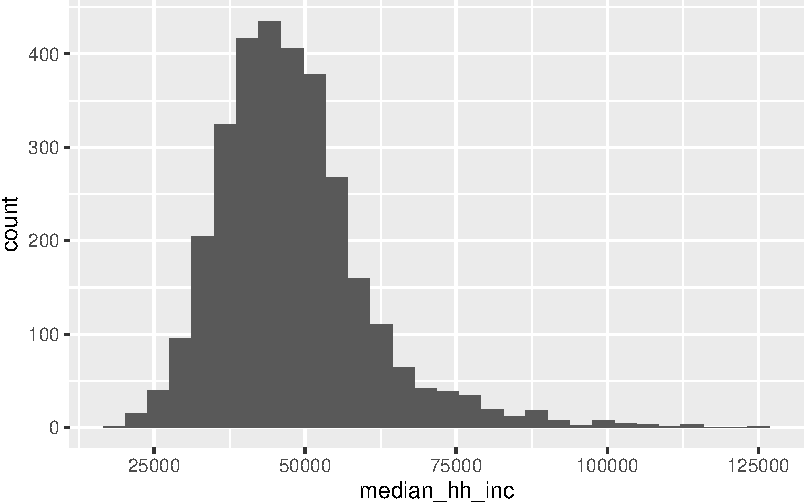
\includegraphics{./12_visualization_files/figure-pdf/unnamed-chunk-3-1.pdf}

}

\end{figure}

Each graph you create using ggplot will contain the following three
elements

\begin{enumerate}
\def\labelenumi{\arabic{enumi}.}
\tightlist
\item
  \textbf{Data}. You need to tell ggplot which data set the variables
  that you want to graph come from. This section is
  \texttt{ggplot(county\_elections)} in the code above.
\item
  \textbf{Aesthetics}. Now that we know which data set we're working
  with, which variables do you want to use and in what way do we want
  them to be used? This information goes in the \texttt{aes()} section.
  Because histograms typically view the distribution of a single
  variable along the x-axis of a graph, we specify our aesthetic
  \texttt{aes(x\ =\ median\_hh\_inc)} in the code above.
\item
  \textbf{Geoms}. The ``geom'' we choose defines the type of graph we're
  ultimately creating (histogram, scatter plot, bar graph, etc). As you
  might expect, \texttt{geom\_histogram()} creates a histogram for us!
\end{enumerate}

In ggplot we combine these elements together using the \texttt{+}
symbol. You could put the data, aesthetics, and geom sections all in the
same line of code. But it is good practice to put each on its own line
to make your code more readable.

Each geom in ggplot has tons of extra options (also called arguments),
which you can specify to make your graphs more pretty. Let's begin to
customize our histogram!

\begin{Shaded}
\begin{Highlighting}[]
\FunctionTok{ggplot}\NormalTok{(county\_elections) }\SpecialCharTok{+}
  \FunctionTok{aes}\NormalTok{(}\AttributeTok{x =}\NormalTok{ median\_hh\_inc) }\SpecialCharTok{+}
  \FunctionTok{geom\_histogram}\NormalTok{(}\AttributeTok{bins =} \DecValTok{50}\NormalTok{,}
                 \AttributeTok{color =} \StringTok{"white"}\NormalTok{,}
                 \AttributeTok{fill =} \StringTok{"steelblue"}\NormalTok{)}
\end{Highlighting}
\end{Shaded}

\begin{figure}[H]

{\centering \includegraphics{./12_visualization_files/figure-pdf/unnamed-chunk-4-1.pdf}

}

\end{figure}

Wow look at that! Now let's fix the ugly default names on the x and y
axes, and add an informative title for our graph. We add custom labels
to a ggplot graph by adding another \texttt{+} followed by a
\texttt{labs()} section.

\begin{Shaded}
\begin{Highlighting}[]
\FunctionTok{ggplot}\NormalTok{(county\_elections) }\SpecialCharTok{+}
  \FunctionTok{aes}\NormalTok{(}\AttributeTok{x =}\NormalTok{ median\_hh\_inc) }\SpecialCharTok{+}
  \FunctionTok{geom\_histogram}\NormalTok{(}\AttributeTok{bins =} \DecValTok{50}\NormalTok{,}
                 \AttributeTok{color =} \StringTok{"white"}\NormalTok{,}
                 \AttributeTok{fill =} \StringTok{"steelblue"}\NormalTok{) }\SpecialCharTok{+}
  \FunctionTok{labs}\NormalTok{(}\AttributeTok{title =} \StringTok{"Distribution of Median County Incomes"}\NormalTok{,}
       \AttributeTok{x =} \StringTok{"Median Household Income"}\NormalTok{,}
       \AttributeTok{y =} \StringTok{"Count"}\NormalTok{)}
\end{Highlighting}
\end{Shaded}

\begin{figure}[H]

{\centering 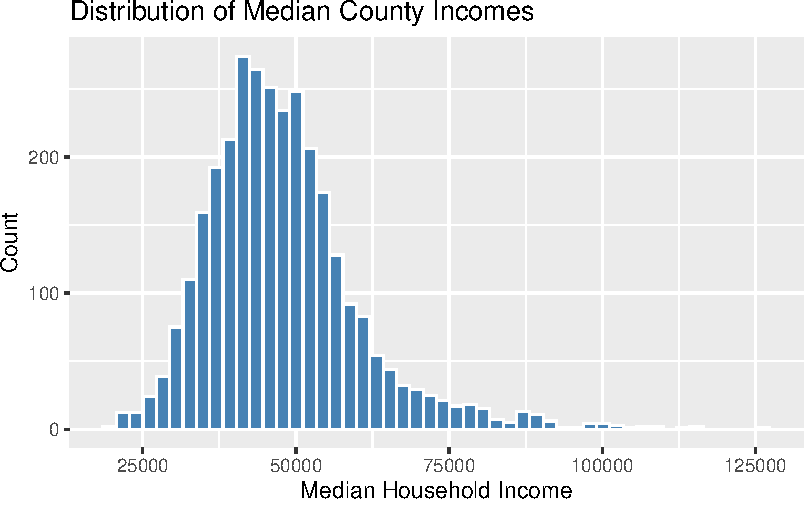
\includegraphics{./12_visualization_files/figure-pdf/unnamed-chunk-5-1.pdf}

}

\end{figure}

Themes in ggplot control the overall look and background style of our
graphs. For a complete list of themes:
\href{https://ggplot2.tidyverse.org/reference/ggtheme.html}{Link}. There
is also a package with a bunch of additional cool themes you can check
out here:
\href{https://yutannihilation.github.io/allYourFigureAreBelongToUs/ggthemes/}{Link}.
Personally I'm a big fan of \texttt{theme\_minimal()}.

\begin{Shaded}
\begin{Highlighting}[]
\FunctionTok{ggplot}\NormalTok{(county\_elections) }\SpecialCharTok{+}
  \FunctionTok{aes}\NormalTok{(}\AttributeTok{x =}\NormalTok{ median\_hh\_inc) }\SpecialCharTok{+}
  \FunctionTok{geom\_histogram}\NormalTok{(}\AttributeTok{bins =} \DecValTok{50}\NormalTok{,}
                 \AttributeTok{color =} \StringTok{"white"}\NormalTok{,}
                 \AttributeTok{fill =} \StringTok{"steelblue"}\NormalTok{) }\SpecialCharTok{+}
  \FunctionTok{labs}\NormalTok{(}\AttributeTok{title =} \StringTok{"Distribution of Median County Incomes"}\NormalTok{,}
       \AttributeTok{x =} \StringTok{"Median Household Income"}\NormalTok{,}
       \AttributeTok{y =} \StringTok{"Count"}\NormalTok{) }\SpecialCharTok{+}
  \FunctionTok{theme\_minimal}\NormalTok{()}
\end{Highlighting}
\end{Shaded}

\begin{figure}[H]

{\centering 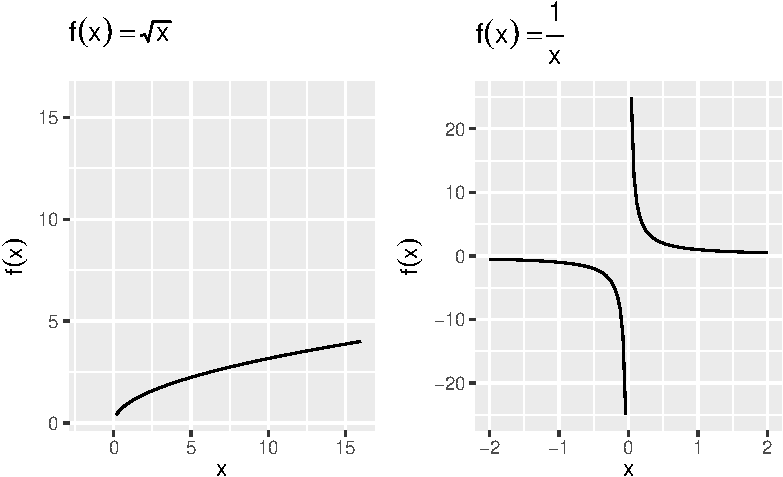
\includegraphics{./12_visualization_files/figure-pdf/unnamed-chunk-6-1.pdf}

}

\end{figure}

Our county median household income variable looks like it's a bit
right-skewed---with a few extremely high income counties shown on the
right hand side of the graph. Depending on your research question, it
might make more sense to view this distribution on the log scale. It's
very easy to do this in ggplot using \texttt{scale\_x\_log10()}.

\begin{Shaded}
\begin{Highlighting}[]
\FunctionTok{ggplot}\NormalTok{(county\_elections) }\SpecialCharTok{+}
  \FunctionTok{aes}\NormalTok{(}\AttributeTok{x =}\NormalTok{ median\_hh\_inc) }\SpecialCharTok{+}
  \FunctionTok{geom\_histogram}\NormalTok{(}\AttributeTok{bins =} \DecValTok{50}\NormalTok{,}
                 \AttributeTok{color =} \StringTok{"white"}\NormalTok{,}
                 \AttributeTok{fill =} \StringTok{"steelblue"}\NormalTok{) }\SpecialCharTok{+}
  \FunctionTok{labs}\NormalTok{(}\AttributeTok{title =} \StringTok{"Distribution of Median County Incomes"}\NormalTok{,}
       \AttributeTok{x =} \StringTok{"Median Household Income"}\NormalTok{,}
       \AttributeTok{y =} \StringTok{""}\NormalTok{,}
       \AttributeTok{caption =} \StringTok{"(log10 scale)"}\NormalTok{) }\SpecialCharTok{+}
  \FunctionTok{theme\_minimal}\NormalTok{() }\SpecialCharTok{+}
  \FunctionTok{scale\_x\_log10}\NormalTok{(}\AttributeTok{labels =}\NormalTok{ scales}\SpecialCharTok{::}\NormalTok{dollar)}
\end{Highlighting}
\end{Shaded}

\begin{figure}[H]

{\centering 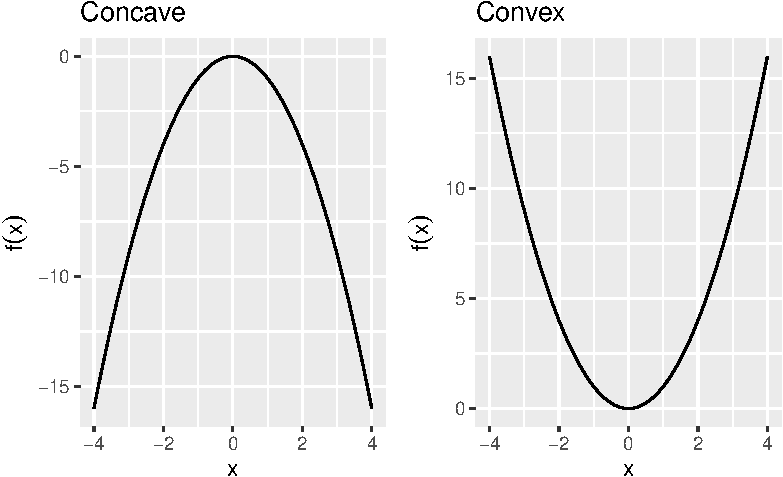
\includegraphics{./12_visualization_files/figure-pdf/unnamed-chunk-7-1.pdf}

}

\end{figure}

Now the data looks almost normally distributed. Also note the use of
\texttt{scales::dollar} to make our x-axis a little easier to read. The
\href{https://scales.r-lib.org/}{scales package} provides a ton of handy
functions to deal with ugly default scales in ggplot. The \texttt{::}
operator is a way of accessing a single function from a package without
loading all its other functions into R. It's also a way of being
explicit about which package's function you are using. Sometimes you
will run across situations where multiple packages have functions with
the same name, but which do different things! Speaking from personal
experience, this can lead to some really frustrating debugging sessions.

\hypertarget{bivariate-graphs}{%
\section{Bivariate Graphs}\label{bivariate-graphs}}

If histograms are the most common way to plot the distribution of a
single continuous variable, scatter plots are the most common way to
show the relationship between two continuous variables. Translating our
histogram ggplot code to a scatter plot is straightforward: simply add a
y-axis variable to \texttt{aes()}, and change the geom to
\texttt{geom\_point()}. The graph below displays the relationship
between median household income and the population percentage in a
county who did not complete high school.

\begin{Shaded}
\begin{Highlighting}[]
\FunctionTok{ggplot}\NormalTok{(county\_elections) }\SpecialCharTok{+}
  \FunctionTok{aes}\NormalTok{(}\AttributeTok{x =}\NormalTok{ median\_hh\_inc, }\AttributeTok{y =}\NormalTok{ lesshs\_pct) }\SpecialCharTok{+}
  \FunctionTok{geom\_point}\NormalTok{()}
\end{Highlighting}
\end{Shaded}

\begin{figure}[H]

{\centering 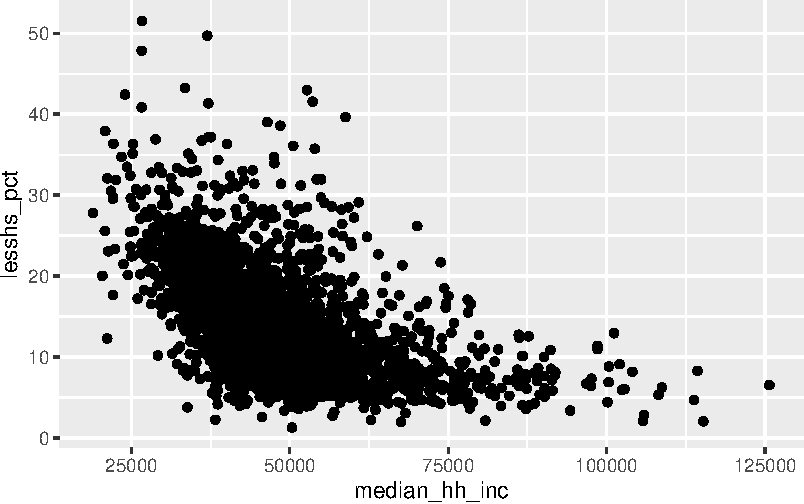
\includegraphics{./12_visualization_files/figure-pdf/unnamed-chunk-8-1.pdf}

}

\end{figure}

It looks like richer counties have lower rates of their population
having less than a high school education. We can use the same
customization options from histograms on our scatter plot to make things
prettier.

\begin{Shaded}
\begin{Highlighting}[]
\FunctionTok{ggplot}\NormalTok{(county\_elections) }\SpecialCharTok{+}
  \FunctionTok{aes}\NormalTok{(}\AttributeTok{x =}\NormalTok{ median\_hh\_inc, }\AttributeTok{y =}\NormalTok{ lesshs\_pct) }\SpecialCharTok{+}
  \FunctionTok{geom\_point}\NormalTok{() }\SpecialCharTok{+}
  \FunctionTok{labs}\NormalTok{(}\AttributeTok{title =} \StringTok{"US Counties by Education and Income"}\NormalTok{,}
       \AttributeTok{x =} \StringTok{"Median Household Income"}\NormalTok{,}
       \AttributeTok{y =} \StringTok{"Less than High School \%"}\NormalTok{) }\SpecialCharTok{+}
  \FunctionTok{scale\_x\_continuous}\NormalTok{(}\AttributeTok{label =}\NormalTok{ scales}\SpecialCharTok{::}\NormalTok{dollar) }\SpecialCharTok{+}
  \FunctionTok{theme\_classic}\NormalTok{()}
\end{Highlighting}
\end{Shaded}

\begin{figure}[H]

{\centering 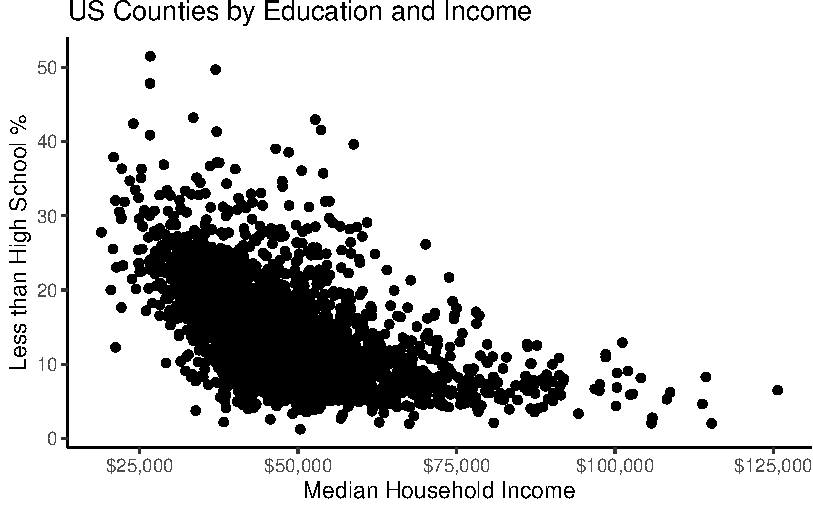
\includegraphics{./12_visualization_files/figure-pdf/unnamed-chunk-9-1.pdf}

}

\end{figure}

A lot of our data seems to be clustered up together. The solid points in
\texttt{geom\_point()} obscure this density so let's fix this using the
\texttt{alpha} argument. A geom's \texttt{alpha} level specifies its
transparency and ranges from 1 (solid) to 0 (invisible).

\begin{Shaded}
\begin{Highlighting}[]
\FunctionTok{ggplot}\NormalTok{(county\_elections) }\SpecialCharTok{+}
  \FunctionTok{aes}\NormalTok{(}\AttributeTok{x =}\NormalTok{ median\_hh\_inc, }\AttributeTok{y =}\NormalTok{ lesshs\_pct) }\SpecialCharTok{+}
  \FunctionTok{geom\_point}\NormalTok{(}\AttributeTok{alpha =} \FloatTok{0.2}\NormalTok{, }\AttributeTok{color =} \StringTok{"darkcyan"}\NormalTok{) }\SpecialCharTok{+}
  \FunctionTok{labs}\NormalTok{(}\AttributeTok{title =} \StringTok{"US Counties by Education and Income"}\NormalTok{,}
       \AttributeTok{x =} \StringTok{"Median Household Income"}\NormalTok{,}
       \AttributeTok{y =} \StringTok{"Less than High School \%"}\NormalTok{) }\SpecialCharTok{+}
  \FunctionTok{scale\_x\_continuous}\NormalTok{(}\AttributeTok{label =}\NormalTok{ scales}\SpecialCharTok{::}\NormalTok{dollar) }\SpecialCharTok{+}
  \FunctionTok{theme\_classic}\NormalTok{()}
\end{Highlighting}
\end{Shaded}

\begin{figure}[H]

{\centering 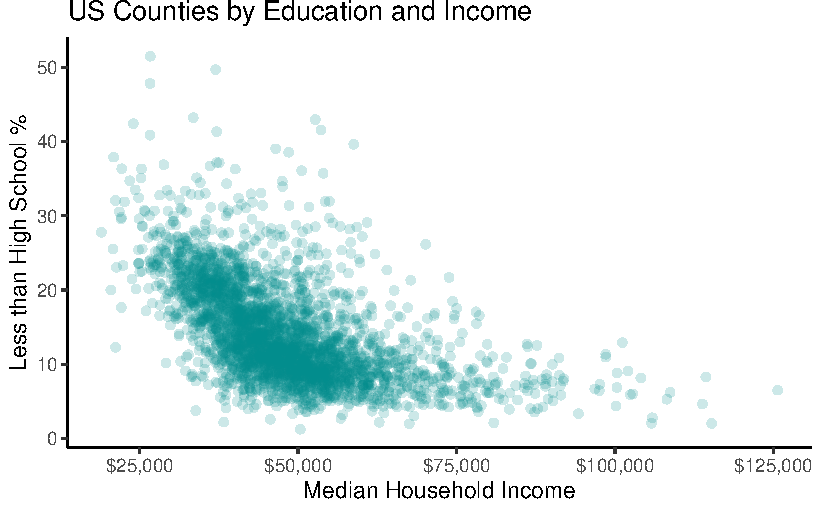
\includegraphics{./12_visualization_files/figure-pdf/unnamed-chunk-10-1.pdf}

}

\end{figure}

The negative relationship between our two variables is clear just by
eyeballing it, but if we want to be real scientists we need to add the
magic regression line. If you are unfamiliar with regression lines,
don't worry---we will be covering them extensively in your introductory
quantitative methods course. A linear regression line is essentially
just the ``best fitting'' straight line to the data.

Adding a regression line to the graph gives us our first opportunity to
combine multiple \emph{geoms}. In the code chunk below, notice how we
simply use \texttt{+} to add \texttt{geom\_smooth()} to our ggplot
object. This overlays a fitted line on top of the dots from
\texttt{geom\_point()}. The argument \texttt{method\ =\ "lm"} tells
ggplot to use a linear regression line (\texttt{lm} = ``linear model'')
as opposed to some other type of fitted line.

\begin{Shaded}
\begin{Highlighting}[]
\FunctionTok{ggplot}\NormalTok{(county\_elections) }\SpecialCharTok{+}
  \FunctionTok{aes}\NormalTok{(}\AttributeTok{x =}\NormalTok{ median\_hh\_inc, }\AttributeTok{y =}\NormalTok{ lesshs\_pct) }\SpecialCharTok{+}
  \FunctionTok{geom\_point}\NormalTok{(}\AttributeTok{alpha =} \FloatTok{0.2}\NormalTok{, }\AttributeTok{color =} \StringTok{"darkcyan"}\NormalTok{) }\SpecialCharTok{+}
  \FunctionTok{geom\_smooth}\NormalTok{(}\AttributeTok{method =} \StringTok{"lm"}\NormalTok{, }\AttributeTok{color =} \StringTok{"black"}\NormalTok{) }\SpecialCharTok{+}
  \FunctionTok{labs}\NormalTok{(}\AttributeTok{title =} \StringTok{"US Counties by Education and Income"}\NormalTok{,}
       \AttributeTok{x =} \StringTok{"Median Household Income"}\NormalTok{,}
       \AttributeTok{y =} \StringTok{"Less than High School \%"}\NormalTok{) }\SpecialCharTok{+}
  \FunctionTok{scale\_x\_continuous}\NormalTok{(}\AttributeTok{label =}\NormalTok{ scales}\SpecialCharTok{::}\NormalTok{dollar) }\SpecialCharTok{+}
  \FunctionTok{theme\_classic}\NormalTok{()}
\end{Highlighting}
\end{Shaded}

\begin{verbatim}
`geom_smooth()` using formula 'y ~ x'
\end{verbatim}

\begin{figure}[H]

{\centering 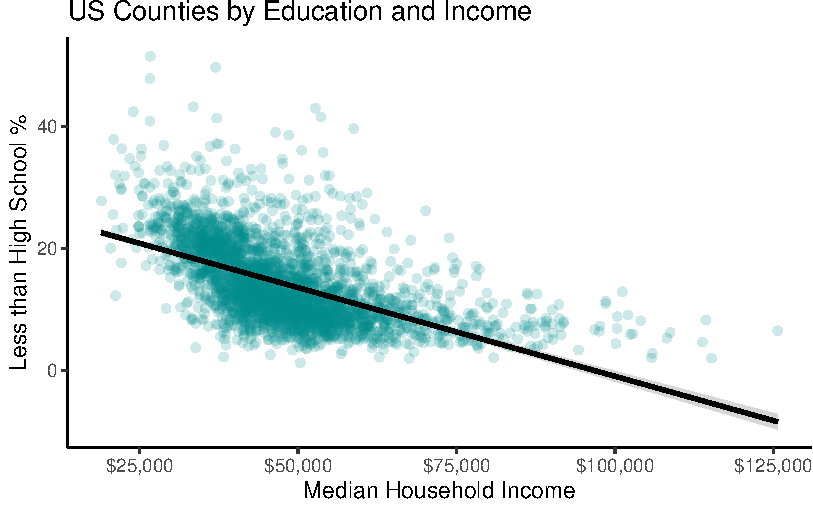
\includegraphics{./12_visualization_files/figure-pdf/unnamed-chunk-11-1.pdf}

}

\end{figure}

This graph would look way more professional if it didn't mistakenly
predict negative high school percentage values for high income counties.
Linear regression is clearly not flexible enough to reflect the true
relationship between our two variables.

What if we re-scaled median household income to the log10 scale again?

\begin{Shaded}
\begin{Highlighting}[]
\FunctionTok{ggplot}\NormalTok{(county\_elections) }\SpecialCharTok{+}
  \FunctionTok{aes}\NormalTok{(}\AttributeTok{x =}\NormalTok{ median\_hh\_inc, }\AttributeTok{y =}\NormalTok{ lesshs\_pct) }\SpecialCharTok{+}
  \FunctionTok{geom\_point}\NormalTok{(}\AttributeTok{alpha =} \FloatTok{0.2}\NormalTok{, }\AttributeTok{color =} \StringTok{"darkcyan"}\NormalTok{) }\SpecialCharTok{+}
  \FunctionTok{geom\_smooth}\NormalTok{(}\AttributeTok{method =} \StringTok{"lm"}\NormalTok{, }\AttributeTok{color =} \StringTok{"black"}\NormalTok{,}
              \AttributeTok{formula =} \StringTok{"y \textasciitilde{} log(x)"}\NormalTok{) }\SpecialCharTok{+}
  \FunctionTok{labs}\NormalTok{(}\AttributeTok{title =} \StringTok{"US Counties by Education and Income"}\NormalTok{,}
       \AttributeTok{x =} \StringTok{"Median Household Income"}\NormalTok{,}
       \AttributeTok{y =} \StringTok{"Less than High School \%"}\NormalTok{) }\SpecialCharTok{+}
  \FunctionTok{scale\_x\_continuous}\NormalTok{(}\AttributeTok{label =}\NormalTok{ scales}\SpecialCharTok{::}\NormalTok{dollar) }\SpecialCharTok{+}
  \FunctionTok{theme\_classic}\NormalTok{()}
\end{Highlighting}
\end{Shaded}

\begin{figure}[H]

{\centering 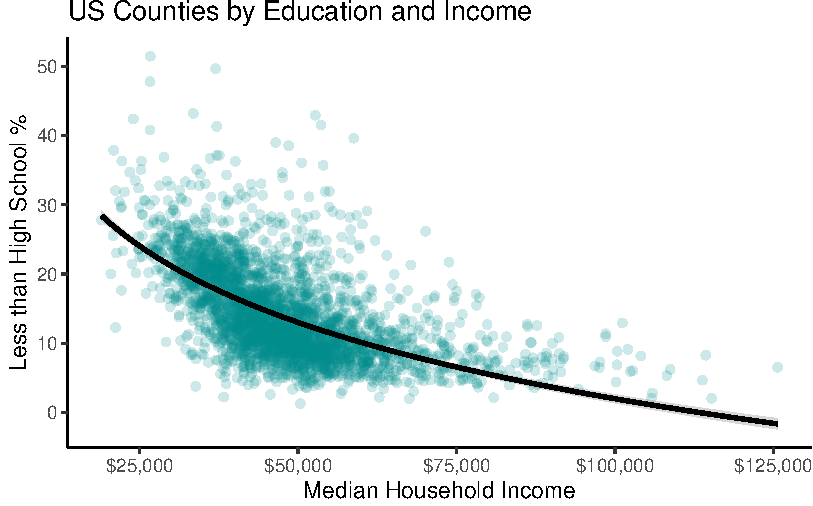
\includegraphics{./12_visualization_files/figure-pdf/unnamed-chunk-12-1.pdf}

}

\end{figure}

Not perfect, but now our fitted line is looking better!

\hypertarget{trivariate-graphs}{%
\section{Trivariate(!) Graphs}\label{trivariate-graphs}}

We are now experts are graphing one variable at a time, or two variables
together, but what if we want to graph three or more variables at once?
There are a number of ways to do this in ggplot as we will see below.
However, first a word of caution: beware of cluttering your plots with
\emph{too} much information! It can be tempting to throw everything into
a graph, but doing so can obscure the main point you're trying to make.
Always keep this in mind when going beyond graphing two variables at
once.

\hypertarget{using-colors-and-shapes}{%
\subsection{Using Colors and Shapes}\label{using-colors-and-shapes}}

The \texttt{county\_elections} data set does not have a lot of
categorical variables for us to work with. So let's create one!

\begin{Shaded}
\begin{Highlighting}[]
\NormalTok{county\_elections }\OtherTok{\textless{}{-}}\NormalTok{ county\_elections }\SpecialCharTok{|\textgreater{}} 
  \FunctionTok{mutate}\NormalTok{(}\AttributeTok{rural =} \FunctionTok{ifelse}\NormalTok{(rural\_pct }\SpecialCharTok{\textgreater{}} \DecValTok{50}\NormalTok{, }\StringTok{"Rural"}\NormalTok{, }\StringTok{"Not Rural"}\NormalTok{))}
\end{Highlighting}
\end{Shaded}

This code chunk uses the \texttt{mutate} function to create a new
variable in the \texttt{county\_elections} data set called
\texttt{rural}. The variable \texttt{rural} takes the value ``Rural'' if
\texttt{rural\_pct} is greater than 50 and takes the value ``Not Rural''
if \texttt{rural\_pct} is less than or equal to 50. It is usually not a
good idea to dichotomize a continuous variable in this way (using a
binary Rural/Not Rural as opposed to the county's rural percentage).
Doing so throws away valuable information that is almost always relevant
to the final analysis. In this case we can justify our choice to create
a categorical variable because it will make plotting multiple variables
much easier.

Let's now take our scatter plot showing the relationship between county
median household income and education level, and color the points based
on whether the county is rural or not. Doing so is as easy as adding
\texttt{color\ =\ rural} to the \texttt{aes()} section in ggplot.

\begin{Shaded}
\begin{Highlighting}[]
\FunctionTok{ggplot}\NormalTok{(county\_elections) }\SpecialCharTok{+}
  \FunctionTok{aes}\NormalTok{(}\AttributeTok{x =}\NormalTok{ median\_hh\_inc, }\AttributeTok{y =}\NormalTok{ lesshs\_pct,}
      \AttributeTok{color =}\NormalTok{ rural) }\SpecialCharTok{+} \CommentTok{\# Coloring points based on rural variable}
  \FunctionTok{geom\_point}\NormalTok{(}\AttributeTok{alpha =} \FloatTok{0.5}\NormalTok{) }\SpecialCharTok{+} \CommentTok{\# Removed color from geom}
  \FunctionTok{labs}\NormalTok{(}\AttributeTok{title =} \StringTok{"US Counties by Education and Income"}\NormalTok{,}
       \AttributeTok{x =} \StringTok{"Median Household Income"}\NormalTok{,}
       \AttributeTok{y =} \StringTok{"Less than High School \%"}\NormalTok{) }\SpecialCharTok{+}
  \FunctionTok{scale\_x\_continuous}\NormalTok{(}\AttributeTok{label =}\NormalTok{ scales}\SpecialCharTok{::}\NormalTok{dollar) }\SpecialCharTok{+}
  \FunctionTok{theme\_classic}\NormalTok{()}
\end{Highlighting}
\end{Shaded}

\begin{figure}[H]

{\centering 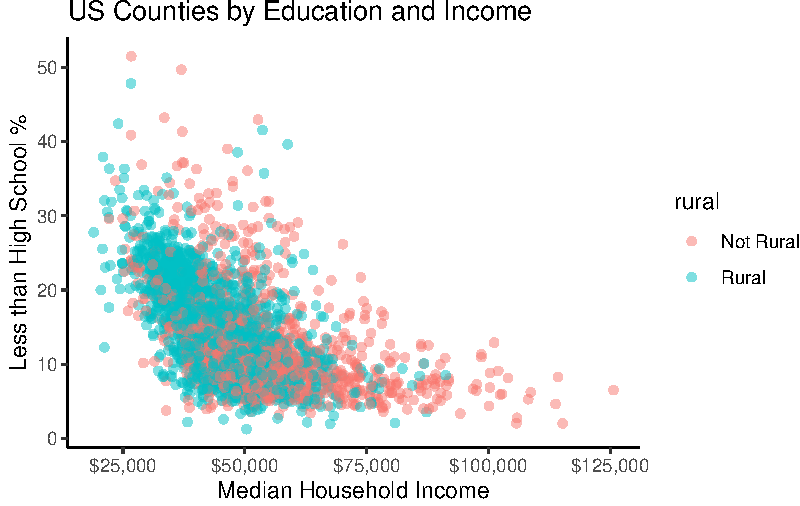
\includegraphics{./12_visualization_files/figure-pdf/unnamed-chunk-14-1.pdf}

}

\end{figure}

By default, ggplot even gives us a handy legend to tell us which color
points correspond to which value of \texttt{rural}.

Now let's try adding a third variable to our scatter plot which is
continuous. One way to do this is with the \texttt{size} option in
\texttt{aes()}.

\begin{Shaded}
\begin{Highlighting}[]
\FunctionTok{ggplot}\NormalTok{(county\_elections) }\SpecialCharTok{+}
  \FunctionTok{aes}\NormalTok{(}\AttributeTok{x =}\NormalTok{ median\_hh\_inc, }\AttributeTok{y =}\NormalTok{ lesshs\_pct,}
      \AttributeTok{size =}\NormalTok{ total\_population) }\SpecialCharTok{+} \CommentTok{\# Changing size of points}
  \FunctionTok{geom\_point}\NormalTok{(}\AttributeTok{alpha =} \FloatTok{0.2}\NormalTok{) }\SpecialCharTok{+} 
  \FunctionTok{labs}\NormalTok{(}\AttributeTok{title =} \StringTok{"US Counties by Education and Income"}\NormalTok{,}
       \AttributeTok{x =} \StringTok{"Median Household Income"}\NormalTok{,}
       \AttributeTok{y =} \StringTok{"Less than High School \%"}\NormalTok{) }\SpecialCharTok{+}
  \FunctionTok{scale\_x\_continuous}\NormalTok{(}\AttributeTok{label =}\NormalTok{ scales}\SpecialCharTok{::}\NormalTok{dollar) }\SpecialCharTok{+}
  \FunctionTok{theme\_classic}\NormalTok{()}
\end{Highlighting}
\end{Shaded}

\begin{figure}[H]

{\centering \includegraphics{./12_visualization_files/figure-pdf/unnamed-chunk-15-1.pdf}

}

\end{figure}

Are we overdoing things with adding too much information to our graph?
Possibly!

\hypertarget{using-facets-to-graph-comparisons}{%
\subsection{Using Facets to Graph
Comparisons}\label{using-facets-to-graph-comparisons}}

One of ggplot's most powerful features is ``faceting''. Facets allow you
to easily graph comparisons between different levels of a categorical
variable in a clear manner by creating side by side subgraphs. To apply
a facet to our ggplot graph we can simply add
\texttt{+\ facet\_wrap(\textasciitilde{}\ facet\_variable)}.

\begin{Shaded}
\begin{Highlighting}[]
\FunctionTok{ggplot}\NormalTok{(county\_elections) }\SpecialCharTok{+}
  \FunctionTok{aes}\NormalTok{(}\AttributeTok{x =}\NormalTok{ median\_hh\_inc, }\AttributeTok{y =}\NormalTok{ lesshs\_pct) }\SpecialCharTok{+}
  \FunctionTok{geom\_point}\NormalTok{(}\AttributeTok{alpha =} \FloatTok{0.2}\NormalTok{, }\AttributeTok{color =} \StringTok{"darkcyan"}\NormalTok{) }\SpecialCharTok{+}
  \FunctionTok{labs}\NormalTok{(}\AttributeTok{title =} \StringTok{"US Counties by Education and Income"}\NormalTok{,}
       \AttributeTok{x =} \StringTok{"Median Household Income"}\NormalTok{,}
       \AttributeTok{y =} \StringTok{"Less than High School \%"}\NormalTok{) }\SpecialCharTok{+}
  \FunctionTok{scale\_x\_continuous}\NormalTok{(}\AttributeTok{label =}\NormalTok{ scales}\SpecialCharTok{::}\NormalTok{dollar) }\SpecialCharTok{+}
  \FunctionTok{theme\_classic}\NormalTok{() }\SpecialCharTok{+}
  \FunctionTok{facet\_wrap}\NormalTok{(}\SpecialCharTok{\textasciitilde{}}\NormalTok{ rural) }\CommentTok{\# Adding faceting}
\end{Highlighting}
\end{Shaded}

\begin{figure}[H]

{\centering \includegraphics{./12_visualization_files/figure-pdf/unnamed-chunk-16-1.pdf}

}

\end{figure}

As you can see, faceting is so powerful for showing comparisons because
it preserves the scale in each subplot. This might be a better choice
rather than coloring each point and overlapping everything. We can
control whether we want the subgraphs side-by-side or on top of each
other with the \texttt{nrow} argument.

\begin{Shaded}
\begin{Highlighting}[]
\FunctionTok{ggplot}\NormalTok{(county\_elections) }\SpecialCharTok{+}
  \FunctionTok{aes}\NormalTok{(}\AttributeTok{x =}\NormalTok{ median\_hh\_inc, }\AttributeTok{y =}\NormalTok{ lesshs\_pct) }\SpecialCharTok{+}
  \FunctionTok{geom\_point}\NormalTok{(}\AttributeTok{alpha =} \FloatTok{0.2}\NormalTok{, }\AttributeTok{color =} \StringTok{"darkcyan"}\NormalTok{) }\SpecialCharTok{+}
  \FunctionTok{labs}\NormalTok{(}\AttributeTok{title =} \StringTok{"US Counties by Education and Income"}\NormalTok{,}
       \AttributeTok{x =} \StringTok{"Median Household Income"}\NormalTok{,}
       \AttributeTok{y =} \StringTok{"Less than High School \%"}\NormalTok{) }\SpecialCharTok{+}
  \FunctionTok{scale\_x\_continuous}\NormalTok{(}\AttributeTok{label =}\NormalTok{ scales}\SpecialCharTok{::}\NormalTok{dollar) }\SpecialCharTok{+}
  \FunctionTok{theme\_classic}\NormalTok{() }\SpecialCharTok{+}
  \FunctionTok{facet\_wrap}\NormalTok{(}\SpecialCharTok{\textasciitilde{}}\NormalTok{ rural, }\AttributeTok{nrow =} \DecValTok{2}\NormalTok{)}
\end{Highlighting}
\end{Shaded}

\begin{figure}[H]

{\centering 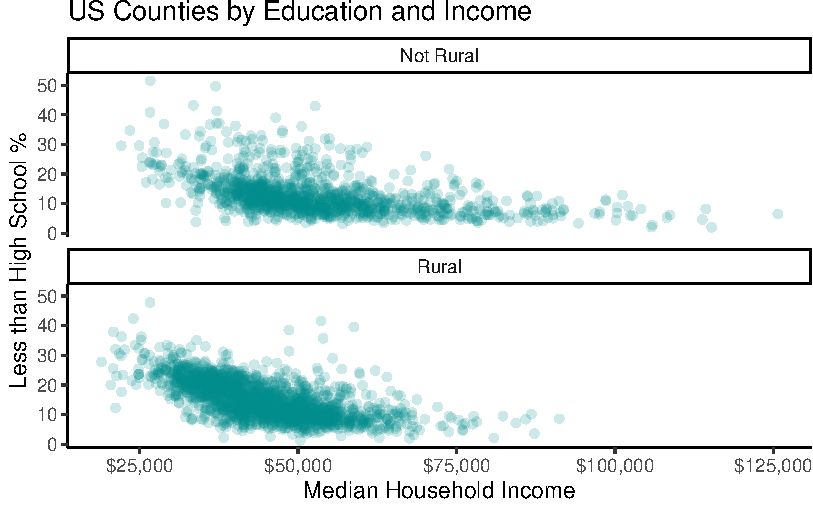
\includegraphics{./12_visualization_files/figure-pdf/unnamed-chunk-17-1.pdf}

}

\end{figure}

\hypertarget{choropleth-maps}{%
\section{Choropleth Maps}\label{choropleth-maps}}

Making maps in ggplot is relatively straightforward---and a much better
idea than copying and pasting your data back and forth between R and a
specialized program like ArcGIS. Choropleth maps show data broken down
by geographic unit (in this case US counties). We will need to install
an additional package
\href{https://urban-institute.medium.com/how-to-create-state-and-county-maps-easily-in-r-577d29300bb2}{urbnmapr}
to help ggplot make this type of graph. To install urbnmapr, run the
following command in your Console.

\begin{Shaded}
\begin{Highlighting}[]
\NormalTok{devtools}\SpecialCharTok{::}\FunctionTok{install\_github}\NormalTok{(}\StringTok{"UrbanInstitute/urbnmapr"}\NormalTok{)}
\end{Highlighting}
\end{Shaded}

We use the command \texttt{devtools::install\_github()} because the
developers of urbnmapr have not submitted their package to the official
CRAN repository. So rather than using \texttt{install.packages} like
we're used to, we instead need to install the package directly from
GitHub. A lot of excellent packages are not available on CRAN, but be
aware that they might not have all the quality-control checks CRAN
packages have.

Once you have the urbnmapr package installed, you can load it into R
using:

\begin{Shaded}
\begin{Highlighting}[]
\FunctionTok{library}\NormalTok{(urbnmapr)}
\end{Highlighting}
\end{Shaded}

We need to perform a couple data cleaning steps before the data is ready
to map in ggplot. The first step is making our \texttt{countyCode}
variable match the format of the corresponding US county code in the
urbnmapr data. US counties are each given a unique 5-digit number called
a
\href{https://www.nrcs.usda.gov/wps/portal/nrcs/detail/national/home/?cid=nrcs143_013697}{FIPS
code}. However, at some point the ``county\_elections.csv'' file was
opened in Excel, which read the FIPS codes as numeric values thereby
removing any 0's from the start of each code. Never open your data in
Excel! Now a bunch of the FIPS codes in our data are only 4-digits long
instead of 5, which means they will not match the FIPS codes in the
urbnmapr data. Luckily we can fix this using the Tidyverse. The function
\texttt{str\_pad} from the
\href{https://stringr.tidyverse.org/}{stringr} package can be used to
``pad'' out a variable with a specific character until it becomes a
specific size.

\begin{Shaded}
\begin{Highlighting}[]
\NormalTok{county\_elections }\OtherTok{\textless{}{-}}\NormalTok{ county\_elections }\SpecialCharTok{|\textgreater{}} 
  \FunctionTok{mutate}\NormalTok{(}\AttributeTok{county\_fips =} \FunctionTok{str\_pad}\NormalTok{(countyCode, }\AttributeTok{width =} \DecValTok{5}\NormalTok{, }\AttributeTok{pad =} \StringTok{"0"}\NormalTok{))}
\end{Highlighting}
\end{Shaded}

Next we need to join our \texttt{county\_elections} data with the
mapping data from urbnmapr. We will do this using a \texttt{left\_join}
command, which, if you are not familiar with, we will cover in much
greater detail in a future lesson. The big idea here is that we have one
data set with county-level variables, such as median household income,
that we need to merge with a data set containing the geographic
coordinate information for each US county.

\begin{Shaded}
\begin{Highlighting}[]
\NormalTok{map\_data }\OtherTok{\textless{}{-}} \FunctionTok{left\_join}\NormalTok{(county\_elections, counties)}
\end{Highlighting}
\end{Shaded}

Awesome! Now we are ready to make a map! Let's check out the geographic
distribution of population percentage without a high school diploma.

\begin{Shaded}
\begin{Highlighting}[]
\FunctionTok{ggplot}\NormalTok{(map\_data) }\SpecialCharTok{+}
  \FunctionTok{aes}\NormalTok{(}\AttributeTok{x =}\NormalTok{ long, }\AttributeTok{y =}\NormalTok{ lat, }
      \AttributeTok{group =}\NormalTok{ group, }\AttributeTok{fill =}\NormalTok{ lesshs\_pct) }\SpecialCharTok{+}
  \FunctionTok{geom\_polygon}\NormalTok{(}\AttributeTok{color =} \ConstantTok{NA}\NormalTok{) }\SpecialCharTok{+}
  \CommentTok{\# This second geom\_polygon shows the state borders}
  \FunctionTok{geom\_polygon}\NormalTok{(}\AttributeTok{data =}\NormalTok{ states, }\AttributeTok{mapping =} \FunctionTok{aes}\NormalTok{(long, lat, }\AttributeTok{group =}\NormalTok{ group),}
               \AttributeTok{fill =} \ConstantTok{NA}\NormalTok{, }\AttributeTok{size =} \FloatTok{0.1}\NormalTok{, }\AttributeTok{color =} \StringTok{"white"}\NormalTok{) }\SpecialCharTok{+}
  \CommentTok{\# Making maps requires you to choose a geographic projection}
  \FunctionTok{coord\_map}\NormalTok{(}\AttributeTok{projection =} \StringTok{"albers"}\NormalTok{, }\AttributeTok{lat0 =} \DecValTok{39}\NormalTok{, }\AttributeTok{lat1 =} \DecValTok{45}\NormalTok{) }\SpecialCharTok{+}
  \CommentTok{\# theme\_void gives us a blank canvas}
  \FunctionTok{theme\_void}\NormalTok{()}
\end{Highlighting}
\end{Shaded}

Don't worry if you are not yet able to understand every aspect of the
ggplot code that produced this map. Try playing around with some of the
arguments and see what happens to the map!

\begin{Shaded}
\begin{Highlighting}[]
\FunctionTok{ggplot}\NormalTok{(map\_data) }\SpecialCharTok{+}
  \FunctionTok{aes}\NormalTok{(}\AttributeTok{x =}\NormalTok{ long, }\AttributeTok{y =}\NormalTok{ lat, }
      \AttributeTok{group =}\NormalTok{ group, }\AttributeTok{fill =}\NormalTok{ lesshs\_pct) }\SpecialCharTok{+}
  \FunctionTok{geom\_polygon}\NormalTok{(}\AttributeTok{color =} \ConstantTok{NA}\NormalTok{) }\SpecialCharTok{+}
  \FunctionTok{geom\_polygon}\NormalTok{(}\AttributeTok{data =}\NormalTok{ states, }\AttributeTok{mapping =} \FunctionTok{aes}\NormalTok{(long, lat, }\AttributeTok{group =}\NormalTok{ group),}
               \AttributeTok{fill =} \ConstantTok{NA}\NormalTok{, }\AttributeTok{size =} \FloatTok{0.1}\NormalTok{, }\AttributeTok{color =} \StringTok{"white"}\NormalTok{) }\SpecialCharTok{+}
  \FunctionTok{coord\_map}\NormalTok{(}\AttributeTok{projection =} \StringTok{"albers"}\NormalTok{, }\AttributeTok{lat0 =} \DecValTok{39}\NormalTok{, }\AttributeTok{lat1 =} \DecValTok{45}\NormalTok{) }\SpecialCharTok{+}
  \CommentTok{\# This creates a diverging color scale}
  \CommentTok{\# that is also colorblind friendly}
  \FunctionTok{scale\_fill\_viridis\_c}\NormalTok{() }\SpecialCharTok{+}
  \FunctionTok{labs}\NormalTok{(}\AttributeTok{fill =} \StringTok{"Less than High School \%"}\NormalTok{) }\SpecialCharTok{+}
  \FunctionTok{theme\_void}\NormalTok{() }\SpecialCharTok{+}
  \FunctionTok{theme}\NormalTok{(}\AttributeTok{legend.position =} \StringTok{"bottom"}\NormalTok{) }
\end{Highlighting}
\end{Shaded}

Sometimes a diverging color scale is better for contrasting high and low
value areas.

\hypertarget{simulation}{%
\chapter{Simulation}\label{simulation}}

Module originally written by Connor Jerzak and Shiro Kuriwaki

\hypertarget{motivation-simulation-as-an-analytical-tool}{%
\subsection*{Motivation: Simulation as an Analytical
Tool}\label{motivation-simulation-as-an-analytical-tool}}
\addcontentsline{toc}{subsection}{Motivation: Simulation as an
Analytical Tool}

An increasing amount of political science contributions now include a
simulation.

\begin{itemize}
\tightlist
\item
  \href{http://www-personal.umich.edu/~axe/research/Dissemination.pdf}{Axelrod
  (1977)} demonstrated via simulation how atomized individuals evolve to
  be grouped in similar clusters or countries, a model of
  culture.\footnote{\href{http://www-personal.umich.edu/~axe/research/Dissemination.pdf}{Axelrod,
    Robert. 1997. ``The Dissemination of Culture.'' \emph{Journal of
    Conflict Resolution} 41(2): 203--26.}}
\item
  \href{http://www-personal.umich.edu/~jowei/florida.pdf}{Chen and
  Rodden (2013)} argued in a 2013 article that the vote-seat inequality
  in U.S. elections that is often attributed to intentional partisan
  gerrymandering can actually attributed to simply the reality of
  ``human geography'' -- Democratic voters tend to be concentrated in
  smaller area. Put another way, no feasible form of gerrymandering
  could spread out Democratic voters in such a way to equalize their
  vote-seat translation effectiveness. After demonstrating the empirical
  pattern of human geography, they advance their key claim by simulating
  thousands of redistricting plans and record the vote-seat
  ratio.\footnote{\href{http://www-personal.umich.edu/~jowei/florida.pdf}{Chen,
    Jowei, and Jonathan Rodden. ``Unintentional Gerrymandering:
    Political Geography and Electoral Bias in Legislatures.
    \emph{Quarterly Journal of Political Science}, 8:239-269''}}
\item
  \href{https://gking.harvard.edu/files/abs/evil-abs.shtml}{Gary King,
  James Honaker, and multiple other authors} propose a way to analyze
  missing data with a method of multiple imputation, which uses a lot of
  simulation from a researcher's observed dataset.\footnote{\href{https://gking.harvard.edu/files/abs/evil-abs.shtml}{King,
    Gary, et al.~``Analyzing Incomplete Political Science Data: An
    Alternative Algorithm for Multiple Imputation''. \emph{American
    Political Science Review}, 95: 49-69.}} (Software:
  Amelia\footnote{\href{http://www.jstatsoft.org/v45/i07/}{James
    Honaker, Gary King, Matthew Blackwell (2011). Amelia II: A Program
    for Missing Data. Journal of Statistical Software, 45(7), 1-47.}})
\end{itemize}

Statistical methods also incorporate simulation:

\begin{itemize}
\tightlist
\item
  The bootstrap: a statistical method for estimating uncertainty around
  some parameter by re-sampling observations.
\item
  Bagging: a method for improving machine learning predictions by
  re-sampling observations, storing the estimate across many re-samples,
  and averaging these estimates to form the final estimate. A variance
  reduction technique.
\item
  Statistical reasoning: if you are trying to understand a quantitative
  problem, a wonderful first-step to understand the problem better is to
  simulate it! The analytical solution is often very hard (or
  impossible), but the simulation is often much easier :-)
\end{itemize}

\hypertarget{where-are-we-where-are-we-headed-1}{%
\subsection*{Where are we? Where are we
headed?}\label{where-are-we-where-are-we-headed-1}}
\addcontentsline{toc}{subsection}{Where are we? Where are we headed?}

Up till now, you should have covered:

\begin{itemize}
\tightlist
\item
  \texttt{R} basics
\item
  Visualization
\item
  Matrices and vectors
\item
  Functions, objects, loops
\item
  Joining real data
\end{itemize}

In this module, we will start to work with generating data within R,
from thin air, as it were. Doing simulation also strengthens your
understanding of Probability.

\hypertarget{check-your-understanding}{%
\subsection*{Check your Understanding}\label{check-your-understanding}}
\addcontentsline{toc}{subsection}{Check your Understanding}

\begin{itemize}
\tightlist
\item
  What does the \texttt{sample()} function do?
\item
  What does \texttt{runif()} stand for?
\item
  What is a \texttt{seed}?
\item
  What is a Monte Carlo?
\end{itemize}

Check if you have an idea of how you might code the following tasks:

\begin{itemize}
\tightlist
\item
  Simulate 100 rolls of a die
\item
  Simulate one random ordering of 25 numbers
\item
  Simulate 100 values of white noise (uniform random variables)
\item
  Generate a ``bootstrap'' sample of an existing dataset
\end{itemize}

We're going to learn about this today!

\hypertarget{pick-a-sample-any-sample}{%
\section{Pick a sample, any sample}\label{pick-a-sample-any-sample}}

\hypertarget{the-sample-function}{%
\section{\texorpdfstring{The \texttt{sample()}
function}{The sample() function}}\label{the-sample-function}}

The core functions for coding up stochastic data revolves around several
key functions, so we will simply review them here.

Suppose you have a vector of values \texttt{x} and from it you want to
randomly sample a sample of length \texttt{size}. For this, use the
\texttt{sample} function

\begin{Shaded}
\begin{Highlighting}[]
\FunctionTok{sample}\NormalTok{(}\AttributeTok{x =} \DecValTok{1}\SpecialCharTok{:}\DecValTok{10}\NormalTok{, }\AttributeTok{size =} \DecValTok{5}\NormalTok{)}
\end{Highlighting}
\end{Shaded}

\begin{verbatim}
[1]  2  4 10  5  1
\end{verbatim}

There are two subtypes of sampling -- with and without replacement.

\begin{enumerate}
\def\labelenumi{\arabic{enumi}.}
\tightlist
\item
  Sampling without replacement (\texttt{replace\ =\ FALSE}) means once
  an element of \texttt{x} is chosen, it will not be considered again:
\end{enumerate}

\begin{Shaded}
\begin{Highlighting}[]
\FunctionTok{sample}\NormalTok{(}\AttributeTok{x =} \DecValTok{1}\SpecialCharTok{:}\DecValTok{10}\NormalTok{, }\AttributeTok{size =} \DecValTok{10}\NormalTok{, }\AttributeTok{replace =} \ConstantTok{FALSE}\NormalTok{) }\DocumentationTok{\#\# no number appears more than once}
\end{Highlighting}
\end{Shaded}

\begin{verbatim}
 [1]  6  7  5  3  2 10  9  8  4  1
\end{verbatim}

\begin{enumerate}
\def\labelenumi{\arabic{enumi}.}
\setcounter{enumi}{1}
\tightlist
\item
  Sampling with replacement (\texttt{replace\ =\ TRUE}) means that even
  if an element of \texttt{x} is chosen, it is put back in the pool and
  may be chosen again.
\end{enumerate}

\begin{Shaded}
\begin{Highlighting}[]
\FunctionTok{sample}\NormalTok{(}\AttributeTok{x =} \DecValTok{1}\SpecialCharTok{:}\DecValTok{10}\NormalTok{, }\AttributeTok{size =} \DecValTok{10}\NormalTok{, }\AttributeTok{replace =} \ConstantTok{TRUE}\NormalTok{) }\DocumentationTok{\#\# any number can appear more than once}
\end{Highlighting}
\end{Shaded}

\begin{verbatim}
 [1]  4  8  7  6  1  5 10  3  8  3
\end{verbatim}

It follows then that you cannot sample without replacement a sample that
is larger than the pool.

\begin{Shaded}
\begin{Highlighting}[]
\FunctionTok{sample}\NormalTok{(}\AttributeTok{x =} \DecValTok{1}\SpecialCharTok{:}\DecValTok{10}\NormalTok{, }\AttributeTok{size =} \DecValTok{100}\NormalTok{, }\AttributeTok{replace =} \ConstantTok{FALSE}\NormalTok{)}
\end{Highlighting}
\end{Shaded}

\begin{verbatim}
Error in sample.int(length(x), size, replace, prob): cannot take a sample larger than the population when 'replace = FALSE'
\end{verbatim}

So far, every element in \texttt{x} has had an equal probability of
being chosen. In some application, we want a sampling scheme where some
elements are more likely to be chosen than others. The argument
\texttt{prob} handles this.

For example, this simulates 20 fair coin tosses (each outcome is equally
likely to happen)

\begin{Shaded}
\begin{Highlighting}[]
\FunctionTok{sample}\NormalTok{(}\FunctionTok{c}\NormalTok{(}\StringTok{"Head"}\NormalTok{, }\StringTok{"Tail"}\NormalTok{), }\AttributeTok{size =} \DecValTok{20}\NormalTok{, }\AttributeTok{prob =} \FunctionTok{c}\NormalTok{(}\FloatTok{0.5}\NormalTok{, }\FloatTok{0.5}\NormalTok{), }\AttributeTok{replace =} \ConstantTok{TRUE}\NormalTok{)}
\end{Highlighting}
\end{Shaded}

\begin{verbatim}
 [1] "Tail" "Tail" "Head" "Head" "Tail" "Head" "Head" "Head" "Tail" "Tail"
[11] "Head" "Head" "Head" "Tail" "Head" "Head" "Head" "Tail" "Head" "Head"
\end{verbatim}

But this simulates 20 biased coin tosses, where say the probability of
Tails is 4 times more likely than the number of Heads

\begin{Shaded}
\begin{Highlighting}[]
\FunctionTok{sample}\NormalTok{(}\FunctionTok{c}\NormalTok{(}\StringTok{"Head"}\NormalTok{, }\StringTok{"Tail"}\NormalTok{), }\AttributeTok{size =} \DecValTok{20}\NormalTok{, }\AttributeTok{prob =} \FunctionTok{c}\NormalTok{(}\FloatTok{0.2}\NormalTok{, }\FloatTok{0.8}\NormalTok{), }\AttributeTok{replace =} \ConstantTok{TRUE}\NormalTok{)}
\end{Highlighting}
\end{Shaded}

\begin{verbatim}
 [1] "Head" "Tail" "Tail" "Tail" "Tail" "Tail" "Tail" "Tail" "Tail" "Tail"
[11] "Tail" "Tail" "Tail" "Head" "Tail" "Head" "Tail" "Tail" "Tail" "Tail"
\end{verbatim}

\hypertarget{sampling-rows-from-a-dataframe}{%
\subsection{Sampling rows from a
dataframe}\label{sampling-rows-from-a-dataframe}}

In tidyverse, there is a convenience function to sample rows randomly:
\texttt{sample\_n()} and \texttt{sample\_frac()}.

For example, load the dataset on cars, \texttt{mtcars}, which has 32
observations.

\begin{Shaded}
\begin{Highlighting}[]
\NormalTok{mtcars}
\end{Highlighting}
\end{Shaded}

\begin{verbatim}
                     mpg cyl  disp  hp drat    wt  qsec vs am gear carb
Mazda RX4           21.0   6 160.0 110 3.90 2.620 16.46  0  1    4    4
Mazda RX4 Wag       21.0   6 160.0 110 3.90 2.875 17.02  0  1    4    4
Datsun 710          22.8   4 108.0  93 3.85 2.320 18.61  1  1    4    1
Hornet 4 Drive      21.4   6 258.0 110 3.08 3.215 19.44  1  0    3    1
Hornet Sportabout   18.7   8 360.0 175 3.15 3.440 17.02  0  0    3    2
Valiant             18.1   6 225.0 105 2.76 3.460 20.22  1  0    3    1
Duster 360          14.3   8 360.0 245 3.21 3.570 15.84  0  0    3    4
Merc 240D           24.4   4 146.7  62 3.69 3.190 20.00  1  0    4    2
Merc 230            22.8   4 140.8  95 3.92 3.150 22.90  1  0    4    2
Merc 280            19.2   6 167.6 123 3.92 3.440 18.30  1  0    4    4
Merc 280C           17.8   6 167.6 123 3.92 3.440 18.90  1  0    4    4
Merc 450SE          16.4   8 275.8 180 3.07 4.070 17.40  0  0    3    3
Merc 450SL          17.3   8 275.8 180 3.07 3.730 17.60  0  0    3    3
Merc 450SLC         15.2   8 275.8 180 3.07 3.780 18.00  0  0    3    3
Cadillac Fleetwood  10.4   8 472.0 205 2.93 5.250 17.98  0  0    3    4
Lincoln Continental 10.4   8 460.0 215 3.00 5.424 17.82  0  0    3    4
Chrysler Imperial   14.7   8 440.0 230 3.23 5.345 17.42  0  0    3    4
Fiat 128            32.4   4  78.7  66 4.08 2.200 19.47  1  1    4    1
Honda Civic         30.4   4  75.7  52 4.93 1.615 18.52  1  1    4    2
Toyota Corolla      33.9   4  71.1  65 4.22 1.835 19.90  1  1    4    1
Toyota Corona       21.5   4 120.1  97 3.70 2.465 20.01  1  0    3    1
Dodge Challenger    15.5   8 318.0 150 2.76 3.520 16.87  0  0    3    2
AMC Javelin         15.2   8 304.0 150 3.15 3.435 17.30  0  0    3    2
Camaro Z28          13.3   8 350.0 245 3.73 3.840 15.41  0  0    3    4
Pontiac Firebird    19.2   8 400.0 175 3.08 3.845 17.05  0  0    3    2
Fiat X1-9           27.3   4  79.0  66 4.08 1.935 18.90  1  1    4    1
Porsche 914-2       26.0   4 120.3  91 4.43 2.140 16.70  0  1    5    2
Lotus Europa        30.4   4  95.1 113 3.77 1.513 16.90  1  1    5    2
Ford Pantera L      15.8   8 351.0 264 4.22 3.170 14.50  0  1    5    4
Ferrari Dino        19.7   6 145.0 175 3.62 2.770 15.50  0  1    5    6
Maserati Bora       15.0   8 301.0 335 3.54 3.570 14.60  0  1    5    8
Volvo 142E          21.4   4 121.0 109 4.11 2.780 18.60  1  1    4    2
\end{verbatim}

sample\_n picks a user-specified number of rows from the dataset:

\begin{Shaded}
\begin{Highlighting}[]
\FunctionTok{sample\_n}\NormalTok{(mtcars, }\DecValTok{3}\NormalTok{)}
\end{Highlighting}
\end{Shaded}

\begin{verbatim}
                mpg cyl  disp  hp drat    wt  qsec vs am gear carb
Fiat 128       32.4   4  78.7  66 4.08 2.200 19.47  1  1    4    1
Toyota Corolla 33.9   4  71.1  65 4.22 1.835 19.90  1  1    4    1
Mazda RX4      21.0   6 160.0 110 3.90 2.620 16.46  0  1    4    4
\end{verbatim}

Sometimes you want a X percent sample of your dataset. In this case use
\texttt{sample\_frac()}

\begin{Shaded}
\begin{Highlighting}[]
\FunctionTok{sample\_frac}\NormalTok{(mtcars, }\FloatTok{0.10}\NormalTok{)}
\end{Highlighting}
\end{Shaded}

\begin{verbatim}
               mpg cyl  disp  hp drat   wt qsec vs am gear carb
Ferrari Dino  19.7   6 145.0 175 3.62 2.77 15.5  0  1    5    6
Maserati Bora 15.0   8 301.0 335 3.54 3.57 14.6  0  1    5    8
Porsche 914-2 26.0   4 120.3  91 4.43 2.14 16.7  0  1    5    2
\end{verbatim}

As a side-note, these functions have very practical uses for any type of
data analysis:

\begin{itemize}
\tightlist
\item
  Inspecting your dataset: using \texttt{head()} all the same time and
  looking over the first few rows might lead you to ignore any issues
  that end up in the bottom for whatever reason.
\item
  Testing your analysis with a small sample: If running analyses on a
  dataset takes more than a handful of seconds, change your dataset
  upstream to a fraction of the size so the rest of the code runs in
  less than a second. Once verifying your analysis code runs, then re-do
  it with your full dataset (by simply removing the \texttt{sample\_n} /
  \texttt{sample\_frac} line of code in the beginning). While three
  seconds may not sound like much, they accumulate and eat up time.
\end{itemize}

\hypertarget{random-numbers-from-specific-distributions}{%
\section{Random numbers from specific
distributions}\label{random-numbers-from-specific-distributions}}

\hypertarget{rbinom}{%
\subsection*{\texorpdfstring{\texttt{rbinom()}}{rbinom()}}\label{rbinom}}
\addcontentsline{toc}{subsection}{\texttt{rbinom()}}

\texttt{rbinom} builds upon \texttt{sample} as a tool to help you answer
the question -- what is the \emph{total number of successes} I would get
if I sampled a binary (Bernoulli) result from a test with \texttt{size}
number of trials each, with a event-wise probability of \texttt{prob}.
The first argument \texttt{n} asks me how many such numbers I want.

For example, I want to know how many Heads I would get if I flipped a
fair coin 100 times.

\begin{Shaded}
\begin{Highlighting}[]
\FunctionTok{rbinom}\NormalTok{(}\AttributeTok{n =} \DecValTok{1}\NormalTok{, }\AttributeTok{size =} \DecValTok{100}\NormalTok{, }\AttributeTok{prob =} \FloatTok{0.5}\NormalTok{)}
\end{Highlighting}
\end{Shaded}

\begin{verbatim}
[1] 55
\end{verbatim}

Now imagine this I wanted to do this experiment 10 times, which would
require I flip the coin 10 x 100 = 1000 times! Helpfully, we can do this
in one line

\begin{Shaded}
\begin{Highlighting}[]
\FunctionTok{rbinom}\NormalTok{(}\AttributeTok{n =} \DecValTok{10}\NormalTok{, }\AttributeTok{size =} \DecValTok{100}\NormalTok{, }\AttributeTok{prob =} \FloatTok{0.5}\NormalTok{)}
\end{Highlighting}
\end{Shaded}

\begin{verbatim}
 [1] 50 58 47 49 54 60 54 50 53 51
\end{verbatim}

\hypertarget{runif}{%
\subsection*{\texorpdfstring{\texttt{runif()}}{runif()}}\label{runif}}
\addcontentsline{toc}{subsection}{\texttt{runif()}}

\texttt{runif} also simulates a stochastic scheme where each event has
equal probability of getting chosen like \texttt{sample}, but is a
continuous rather than discrete system. We will cover this more in the
next math module.

The intuition to emphasize here is that one can generate potentially
infinite amounts (size \texttt{n}) of noise that is a essentially random

\begin{Shaded}
\begin{Highlighting}[]
\FunctionTok{runif}\NormalTok{(}\AttributeTok{n =} \DecValTok{5}\NormalTok{)}
\end{Highlighting}
\end{Shaded}

\begin{verbatim}
[1] 0.57343306 0.60872460 0.52434672 0.09688019 0.46674553
\end{verbatim}

\hypertarget{rnorm}{%
\subsection*{\texorpdfstring{\texttt{rnorm()}}{rnorm()}}\label{rnorm}}
\addcontentsline{toc}{subsection}{\texttt{rnorm()}}

\texttt{rnorm} is also a continuous distribution, but draws from a
Normal distribution -- perhaps the most important distribution in
statistics. It runs the same way as \texttt{runif}

\begin{Shaded}
\begin{Highlighting}[]
\FunctionTok{rnorm}\NormalTok{(}\AttributeTok{n =} \DecValTok{5}\NormalTok{)}
\end{Highlighting}
\end{Shaded}

\begin{verbatim}
[1]  0.04014912 -1.33034698 -1.24651827  1.82108817  0.95616967
\end{verbatim}

To better visualize the difference between the output of \texttt{runif}
and \texttt{rnorm}, let's generate lots of each and plot a histogram.

\begin{Shaded}
\begin{Highlighting}[]
\NormalTok{from\_runif }\OtherTok{\textless{}{-}} \FunctionTok{runif}\NormalTok{(}\AttributeTok{n =} \DecValTok{1000}\NormalTok{)}
\NormalTok{from\_rnorm }\OtherTok{\textless{}{-}} \FunctionTok{rnorm}\NormalTok{(}\AttributeTok{n =} \DecValTok{1000}\NormalTok{)}

\FunctionTok{par}\NormalTok{(}\AttributeTok{mfrow =} \FunctionTok{c}\NormalTok{(}\DecValTok{1}\NormalTok{, }\DecValTok{2}\NormalTok{)) }\DocumentationTok{\#\# base{-}R parameter for two plots at once}
\FunctionTok{hist}\NormalTok{(from\_runif)}
\FunctionTok{hist}\NormalTok{(from\_rnorm)}
\end{Highlighting}
\end{Shaded}

\begin{figure}[H]

{\centering \includegraphics{./14_simulation_files/figure-pdf/unnamed-chunk-15-1.pdf}

}

\end{figure}

\hypertarget{r-p-and-d}{%
\section{r, p, and d}\label{r-p-and-d}}

Each distribution can do more than generate random numbers (the prefix
\texttt{r}). We can compute the cumulative probability by the function
\texttt{pbinom()}, \texttt{punif()}, and \texttt{pnorm()}. Also the
density -- the value of the PDF -- by \texttt{dbinom()},
\texttt{dunif()} and \texttt{dnorm()}.

\hypertarget{set.seed}{%
\section{\texorpdfstring{\texttt{set.seed()}}{set.seed()}}\label{set.seed}}

\texttt{R} doesn't have the ability to generate truly random numbers!
Random numbers are actually very hard to generate. (Think: flipping a
coin --\textgreater{} can be perfectly predicted if I know wind speed,
the angle the coin is flipped, etc.). Some people use random noise in
the atmosphere or random behavior in quantum systems to generate
``truly'' (?) random numbers. Conversely, R uses deterministic
algorithms which take as an input a ``seed'' and which then perform a
series of operations to generate a sequence of random-seeming numbers
(that is, numbers whose sequence is sufficiently hard to predict).

Let's think about this another way. Sampling is a stochastic process, so
every time you run \texttt{sample()} or \texttt{runif()} you are bound
to get a different output (because different random seeds are used).
This is intentional in some cases but you might want to avoid it in
others. For example, you might want to diagnose a coding discrepancy by
setting the random number generator to give the same number each time.
To do this, use the function \texttt{set.seed()}.

In the function goes any number. When you run a sample function in the
same command as a preceding \texttt{set.seed()}, the sampling function
will always give you the same sequence of numbers. In a sense, the
sampler is no longer random (in the sense of unpredictable to use;
remember: it never was ``truly'' random in the first place)

\begin{Shaded}
\begin{Highlighting}[]
\FunctionTok{set.seed}\NormalTok{(}\DecValTok{02138}\NormalTok{)}
\FunctionTok{runif}\NormalTok{(}\AttributeTok{n =} \DecValTok{10}\NormalTok{)}
\end{Highlighting}
\end{Shaded}

\begin{verbatim}
 [1] 0.51236144 0.61530551 0.37451441 0.43541258 0.21166530 0.17812129
 [7] 0.04420775 0.45567854 0.88718264 0.06970056
\end{verbatim}

The random number generator should give you the exact same sequence of
numbers if you precede the function by the same seed,

\begin{Shaded}
\begin{Highlighting}[]
\FunctionTok{set.seed}\NormalTok{(}\DecValTok{02138}\NormalTok{)}
\FunctionTok{runif}\NormalTok{(}\AttributeTok{n =} \DecValTok{10}\NormalTok{)}
\end{Highlighting}
\end{Shaded}

\begin{verbatim}
 [1] 0.51236144 0.61530551 0.37451441 0.43541258 0.21166530 0.17812129
 [7] 0.04420775 0.45567854 0.88718264 0.06970056
\end{verbatim}

\hypertarget{exercises-1}{%
\section*{Exercises}\label{exercises-1}}
\addcontentsline{toc}{section}{Exercises}

\hypertarget{census-sampling}{%
\subsection*{Census Sampling}\label{census-sampling}}
\addcontentsline{toc}{subsection}{Census Sampling}

What can we learn from surveys of populations, and how wrong do we get
if our sampling is biased?\footnote{This example is inspired from
  \href{https://statistics.fas.harvard.edu/files/statistics-2/files/statistical_paradises_and_paradoxes.pdf}{Meng,
  Xiao-Li (2018). Statistical paradises and paradoxes in big data (I):
  Law of large populations, big data paradox, and the 2016 US
  presidential election. \emph{Annals of Applied Statistics} 12:2,
  685--726. doi:10.1214/18-AOAS1161SF.}} Suppose we want to estimate the
proportion of U.S. residents who are non-white
(\texttt{race\ !=\ "White"}). In reality, we do not have any population
dataset to utilize and so we \emph{only see the sample survey}. Here,
however, to understand how sampling works, let's conveniently use the
Census extract in some cases and pretend we didn't in others.

\begin{enumerate}
\def\labelenumi{(\alph{enumi})}
\tightlist
\item
  First, load \texttt{usc2010\_001percent.csv} into your R session.
  After loading the \texttt{library(tidyverse)}, browse it. Although
  this is only a 0.01 percent extract, treat this as your population for
  pedagogical purposes. What is the population proportion of non-White
  residents?
\end{enumerate}

\begin{enumerate}
\def\labelenumi{(\alph{enumi})}
\setcounter{enumi}{1}
\tightlist
\item
  Setting a seed to \texttt{1669482}, sample 100 respondents from this
  sample. What is the proportion of non-White residents in this
  \emph{particular} sample? By how many percentage points are you off
  from (what we labelled as) the true proportion?
\end{enumerate}

\begin{enumerate}
\def\labelenumi{(\alph{enumi})}
\setcounter{enumi}{2}
\tightlist
\item
  Now imagine what you did above was one survey. What would we get if we
  did 20 surveys?
\end{enumerate}

To simulate this, write a loop that does the same exercise 20 times,
each time computing a sample proportion. Use the same seed at the top,
but be careful to position the \texttt{set.seed} function such that it
generates the same sequence of 20 samples, rather than 20 of the same
sample.

Try doing this with a \texttt{for} loop and storing your sample
proportions in a new length-20 vector. (Suggestion: make an empty vector
first as a container). After running the loop, show a histogram of the
20 values. Also what is the average of the 20 sample estimates?

\begin{enumerate}
\def\labelenumi{(\alph{enumi})}
\setcounter{enumi}{3}
\tightlist
\item
  Now, to make things more real, let's introduce some response bias. The
  goal here is not to correct response bias but to induce it and see how
  it affects our estimates. Suppose that non-White residents are 10
  percent less likely to respond to enter your survey than White
  respondents. This is plausible if you think that the Census is from
  2010 but you are polling in 2018, and racial minorities are more
  geographically mobile than Whites. Repeat the same exercise in (c) by
  modeling this behavior.
\end{enumerate}

You can do this by creating a variable, e.g.~\texttt{propensity}, that
is 0.9 for non-Whites and 1 otherwise. Then, you can refer to it in the
propensity argument.

\begin{enumerate}
\def\labelenumi{(\alph{enumi})}
\setcounter{enumi}{4}
\tightlist
\item
  Finally, we want to see if more data (``Big Data'') will improve our
  estimates. Using the same unequal response rates framework as (d),
  repeat the same exercise but instead of each poll collecting 100
  responses, we collect 10,000.
\end{enumerate}

\begin{enumerate}
\def\labelenumi{(\alph{enumi})}
\setcounter{enumi}{5}
\tightlist
\item
  Optional - visualize your 2 pairs of 20 estimates, with a bar showing
  the ``correct'' population average.
\end{enumerate}

\hypertarget{conditional-proportions}{%
\subsection*{Conditional Proportions}\label{conditional-proportions}}
\addcontentsline{toc}{subsection}{Conditional Proportions}

This example is not on simulation, but is meant to reinforce some of the
probability discussion from math lecture.

Read in the Upshot Siena poll from Fall 2016,
\texttt{data/input/upshot-siena-polls.csv}.

In addition to some standard demographic questions, we will focus on one
called \texttt{vt\_pres\_2} in the csv. This is a two-way presidential
vote question, asking respondents who they plan to vote for President if
the election were held today -- Donald Trump, the Republican, or Hilary
Clinton, the Democrat, with options for Other candidates as well. For
this problem, use the two-way vote question rather than the 4-way vote
question.

\begin{enumerate}
\def\labelenumi{(\alph{enumi})}
\tightlist
\item
  Drop the the respondents who answered the November poll (i.e.~those
  for which \texttt{poll\ ==\ "November"}). We do this in order to
  ignore this November population in all subsequent parts of this
  question because they were not asked the Presidential vote question.
\end{enumerate}

\begin{enumerate}
\def\labelenumi{(\alph{enumi})}
\setcounter{enumi}{1}
\tightlist
\item
  Using the dataset after the procedure in (a), find the proportion of
  \emph{poll respondents} (those who are in the sample) who support
  Donald Trump.
\end{enumerate}

\begin{enumerate}
\def\labelenumi{(\alph{enumi})}
\setcounter{enumi}{2}
\item
  Among those who supported Donald Trump, what proportion of them has a
  Bachelor's degree or higher (i.e.~have a Bachelor's, Graduate, or
  other Professional Degree)?
\item
  Among those who did not support Donald Trump (i.e.~including
  supporters of Hilary Clinton, another candidate, or those who refused
  to answer the question), what proportion of them has a Bachelor's
  degree or higher?
\item
  Express the numbers in the previous parts as probabilities of
  specified events. Define your own symbols: For example, we can let
  \(T\) be the event that a randomly selected respondent in the poll
  supports Donald Trump, then the proportion in part (b) is the
  probability \(P(T).\)
\item
  Suppose we randomly sampled a person who participated in the survey
  and found that he/she had a Bachelor's degree or higher. Given this
  evidence, what is the probability that the same person supports Donald
  Trump? Use Bayes Rule and show your work -- that is, do not use data
  or R to compute the quantity directly. Then, verify this is the case
  via R.
\end{enumerate}

\hypertarget{the-birthday-problem}{%
\subsection*{The Birthday problem}\label{the-birthday-problem}}
\addcontentsline{toc}{subsection}{The Birthday problem}

Write code that will answer the well-known birthday problem via
simulation.\footnote{This exercise draws from Imai (2017)}

The problem is fairly simple: Suppose \(k\) people gather together in a
room. What is the probability at least two people share the same
birthday?

To simplify reality a bit, assume that (1) there are no leap years, and
so there are always 365 days in a year, and (2) a given individual's
birthday is randomly assigned and independent from each other.

\emph{Step 1}: Set \texttt{k} to a concrete number. Pick a number from 1
to 365 randomly, \texttt{k} times to simulate birthdays (would this be
with replacement or without?).

\begin{Shaded}
\begin{Highlighting}[]
\CommentTok{\# Your code}
\end{Highlighting}
\end{Shaded}

\emph{Step 2}: Write a line (or two) of code that gives a \texttt{TRUE}
or \texttt{FALSE} statement of whether or not at least two people share
the same birth date.

\begin{Shaded}
\begin{Highlighting}[]
\CommentTok{\# Your code}
\end{Highlighting}
\end{Shaded}

\emph{Step 3}: The above steps will generate a \texttt{TRUE} or
\texttt{FALSE} answer for your event of interest, but only for one
realization of an event in the sample space. In order to estimate the
\emph{probability} of your event happening, we need a ``stochastic'', as
opposed to ``deterministic'', method. To do this, write a loop that does
Steps 1 and 2 repeatedly for many times, call that number of times
\texttt{sims}. For each of \texttt{sims} iteration, your code should
give you a \texttt{TRUE} or \texttt{FALSE} answer. Code up a way to
store these estimates.

\begin{Shaded}
\begin{Highlighting}[]
\CommentTok{\# Your code}
\end{Highlighting}
\end{Shaded}

\emph{Step 4}: Finally, generalize the function further by letting
\texttt{k} be a user-defined number. You have now created a \emph{Monte
Carlo simulation}!

\begin{Shaded}
\begin{Highlighting}[]
\CommentTok{\# Your code}
\end{Highlighting}
\end{Shaded}

\emph{Step 5}: Generate a table or plot that shows how the probability
of sharing a birthday changes by \texttt{k} (fixing \texttt{sims} at a
large number like \texttt{1000}). Also generate a similar plot that
shows how the probability of sharing a birthday changes by \texttt{sims}
(fixing \texttt{k} at some arbitrary number like \texttt{10}).

\begin{Shaded}
\begin{Highlighting}[]
\CommentTok{\# Your code}
\end{Highlighting}
\end{Shaded}

\emph{Extra credit}: Give an ``analytical'' answer to this problem, that
is an answer through deriving the mathematical expressions of the
probability.

\begin{Shaded}
\begin{Highlighting}[]
\CommentTok{\# Your equations}
\end{Highlighting}
\end{Shaded}

\hypertarget{nonwysiwyg}{%
\chapter{LaTeX and Markdown}\label{nonwysiwyg}}

\hypertarget{where-are-we-where-are-we-headed-2}{%
\subsection*{Where are we? Where are we
headed?}\label{where-are-we-where-are-we-headed-2}}
\addcontentsline{toc}{subsection}{Where are we? Where are we headed?}

Up till now, you should have covered:

\begin{itemize}
\tightlist
\item
  Statistical Programming in \texttt{R}
\end{itemize}

This is only the beginning of \texttt{R} -- programming is like learning
a language, so learn more as we use it. And yet \texttt{R} is of likely
not the only programming language you will want to use. While we cannot
introduce everything, we'll pick out a few that we think are
particularly helpful.

Here will cover

\begin{itemize}
\tightlist
\item
  Markdown
\item
  LaTeX (and BibTeX)
\end{itemize}

as examples of a non-WYSIWYG editor

command-line are a basic set of tools that you may have to use from time
to time. It also clarifies what more complicated programs are doing.
Markdown is an example of compiling a plain text file. LaTeX is a
typesetting program and git is a version control program -- both are
useful for non-quantitative work as well.

Please familiarize yourself closing with Markdown, and be sure you know
how to open an .Rmd file as described below. In class, we will walk
through an Rmd file together. LaTeX is included here for your future
reference as this is a popular typesetting program among political
scientists. This is not needed for Math Camp and is never required for
any course. In fact, many prefer R Markdown's integration rather than a
separate typesetting program. This depends on your background and
interests but exposure to the range of popular programs and techniques
will be helpful moving forward.

\hypertarget{check-your-understanding-1}{%
\subsection*{Check your
understanding}\label{check-your-understanding-1}}
\addcontentsline{toc}{subsection}{Check your understanding}

Check if you have an idea of how you might code the following tasks:

\begin{itemize}
\tightlist
\item
  What does ``WYSIWYG'' stand for? How would a non-WYSIWYG format text?
\item
  How do you start a header in markdown?
\item
  What are some ``plain text'' editors?
\item
  How do you start a document in \texttt{.tex}?
\item
  How do you start a environment in \texttt{.tex}?
\item
  How do you insert a figure in \texttt{.tex}?
\item
  How do you reference a figure in \texttt{.tex}?
\item
  What is a \texttt{.bib} file?
\item
  Say you came across a interesting journal article. How would you want
  to maintain this reference so that you can refer to its citation in
  all your subsequent papers?
\end{itemize}

\hypertarget{motivation}{%
\section{Motivation}\label{motivation}}

Statistical programming is a fast-moving field. The beta version of
\texttt{R} was released in 2000, \texttt{ggplot2} was released on 2005,
and \texttt{RStudio} started around 2010. Of course, some programming
technologies are quite ``old'': (\texttt{C} in 1969, \texttt{C++} around
1989, \texttt{TeX} in 1978, \texttt{Linux} in 1991, Mac OS in 1984). But
it is easy to feel you are falling behind in the recent developments of
programming. Today we will do a \textbf{brief} and rough overview of
some fundamental and new tools other than \texttt{R}, with the general
aim of having you break out of your comfort zone so you won't be shut
out from learning these tools in the future.

\hypertarget{markdown}{%
\section{Markdown}\label{markdown}}

At its core markdown is just plain text. Plain text does not have any
formatting embedded in it. Instead, the formatting is coded up as text.
Markdown is \emph{not} a WYSIWYG (What you see is what you get) text
editor like Microsoft Word or Google Docs. This will mean that you need
to explicitly code for \texttt{bold\{text\}} rather than hitting
Command+B and making your text look \textbf{bold} on your own computer.

Markdown is known as a ``light-weight'' editor, which means that it is
relatively easy to write code that will compile. It is quick and easy
and satisfies most presentation purposes; you might want to try
\texttt{LaTeX} for more involved papers.

\hypertarget{markdown-commands}{%
\subsection{markdown commands}\label{markdown-commands}}

For italic and bold, use either the asterisks or the underlines,

\begin{verbatim}
*italic*   **bold**
_italic_   __bold__
\end{verbatim}

And for headers use the hash symbols,

\begin{verbatim}
# Main Header
## Sub-headers
\end{verbatim}

\hypertarget{your-own-markdown}{%
\subsection{your own markdown}\label{your-own-markdown}}

RStudio makes it easy to compile your very first markdown file by giving
you templates. Got to \texttt{New\ \textgreater{}\ R\ Markdown}, pick a
document and click Ok. This will give you a skeleton of a document you
can compile -- or ``knit''.

Rmd is actually a slight modification of real markdown. It is a type of
file that R reads and turns into a proper \texttt{md} file. Then, it
uses a document-conversion called pandoc to compile your \texttt{md}
into documents like PDF or HTML.

\begin{figure}

{\centering 
\includegraphics{./images/RMarkdownFlow.png}

}

\caption{How Rmds become PDFs or HTMLs}

\end{figure}

\hypertarget{a-note-on-plain-text-editors}{%
\subsection{A note on plain-text
editors}\label{a-note-on-plain-text-editors}}

Multiple software exist where you can edit plain-text (roughly speaking,
text that is not WYSIWYG).

\begin{itemize}
\tightlist
\item
  RStudio (especially for R-related links)
\item
  TeXMaker, TeXShop (especially for TeX)
\item
  \href{https://www.gnu.org/software/emacs/}{emacs}, aquamacs (general)
\item
  \href{http://www.vim.org/download.php}{vim} (general)
\item
  \href{https://www.sublimetext.com}{Sublime Text} (general)
\item
  \href{https://atom.io/}{Atom} (general)
\end{itemize}

Each has their own keyboard shortcuts and special features. You can
browse a couple and see which one(s) you like.

\hypertarget{latex}{%
\section{LaTeX}\label{latex}}

LaTeX is a typesetting program. You'd engage with LaTeX much like you
engage with your \texttt{R} code. You will interact with LaTeX in a text
editor, and will writing code which will be interpreted by the LaTeX
compiler and which will finally be parsed to form your final PDF.

\hypertarget{compile-online}{%
\subsection{compile online}\label{compile-online}}

\begin{enumerate}
\def\labelenumi{\arabic{enumi}.}
\tightlist
\item
  Go to \url{https://www.overleaf.com}
\item
  Scroll down and go to ``CREATE A NEW PAPER'' if you don't have an
  account.
\item
  Let's discuss the default template.
\item
  Make a new document, and set it as your main document. Then type in
  the Minimal Working Example (MWE):
\end{enumerate}

\begin{Shaded}
\begin{Highlighting}[]
\ExtensionTok{\textbackslash{}documentclass\{article\}}
\ExtensionTok{\textbackslash{}begin\{document\}}
\ExtensionTok{Hello}\NormalTok{ World}
\ExtensionTok{\textbackslash{}end\{document\}}
\end{Highlighting}
\end{Shaded}

\hypertarget{compile-your-first-latex-document-locally}{%
\subsection{compile your first LaTeX document
locally}\label{compile-your-first-latex-document-locally}}

LaTeX is a very stable system, and few changes to it have been made
since the 1990s. The main benefit: better control over how your papers
will look; better methods for writing equations or making tables;
overall pleasing aesthetic.

\begin{enumerate}
\def\labelenumi{\arabic{enumi}.}
\tightlist
\item
  Open a plain text editor. Then type in the MWE
\end{enumerate}

\begin{Shaded}
\begin{Highlighting}[]
\ExtensionTok{\textbackslash{}documentclass\{article\}}
\ExtensionTok{\textbackslash{}begin\{document\}}
\ExtensionTok{Hello}\NormalTok{ World}
\ExtensionTok{\textbackslash{}end\{document\}}
\end{Highlighting}
\end{Shaded}

\begin{enumerate}
\def\labelenumi{\arabic{enumi}.}
\setcounter{enumi}{1}
\tightlist
\item
  Save this as \texttt{hello\_world.tex}. Make sure you get the file
  extension right.
\item
  Open this in your ``LaTeX'' editor. This can be \texttt{TeXMaker},
  \texttt{Aqumacs}, etc..
\item
  Go through the click/dropdown interface and click compile.
\end{enumerate}

\hypertarget{main-latex-commands}{%
\subsection{main LaTeX commands}\label{main-latex-commands}}

LaTeX can cover most of your typesetting needs, to clean equations and
intricate diagrams.

Some main commands you'll be using are below, and a very concise cheat
sheet here: \url{https://wch.github.io/latexsheet/latexsheet.pdf}

Most involved features require that you begin a specific ``environment''
for that feature, clearly demarcating them by the notation
\texttt{\textbackslash{}begin\{figure\}} and then
\texttt{\textbackslash{}end\{figure\}}, e.g.~in the case of figures.

\begin{verbatim}
\begin{figure}
\includegraphics{histogram.pdf}
\end{figure}
\end{verbatim}

where \texttt{histogram.pdf} is a path to one of your files.

Notice that each line starts with a backslash \texttt{\textbackslash{}}
-- in LaTeX this is the symbol to run a command.

The following syntax at the endpoints are shorthand for math equations.

\begin{verbatim}
\[\int x^2 dx\]
\end{verbatim}

these compile math symbols: \(\displaystyle \int x^2 dx.\)\footnote{Enclosing
  with \texttt{\$\$} instead of \texttt{\textbackslash{}{[}} also has
  the same effect, so you may see it too. But this is now discouraged
  due to its inflexibility.}

The \texttt{align} environment is useful to align your multi-line math,
for example.

\begin{verbatim}
\begin{align}
P(A \mid B) &= \frac{P(A \cap B)}{P(B)}\\
&= \frac{P(B \mid A)P(A)}{P(B)}
\end{align}
\end{verbatim}

\begin{align}
P(A \mid B) &= \frac{P(A \cap B)}{P(B)}\\
&= \frac{P(B \mid A)P(A)}{P(B)}
\end{align}

Regression tables should be outputted as \texttt{.tex} files with
packages like \texttt{xtable} and \texttt{stargazer}, and then called
into LaTeX by \texttt{\textbackslash{}input\{regression\_table.tex\}}
where \texttt{regression\_table.tex} is the path to your regression
output.

Figures and equations should be labelled with the tag
(e.g.~\texttt{label\{tab:regression\}} so that you can refer to them
later with their tag
\texttt{Table\ \textbackslash{}ref\{tab:regression\}}, instead of
hard-coding \texttt{Table\ 2}).

For some LaTeX commands you might need to load a separate package that
someone else has written. Do this in your preamble (i.e.~before
\texttt{\textbackslash{}begin\{document\}}):

\begin{verbatim}
\usepackage[options]{package}
\end{verbatim}

where \texttt{package} is the name of the package and \texttt{options}
are options specific to the package.

\hypertarget{further-guides}{%
\subsection*{Further Guides}\label{further-guides}}
\addcontentsline{toc}{subsection}{Further Guides}

For a more comprehensive listing of LaTeX commands, Mayya Komisarchik
has a great tutorial set of folders:
\url{https://scholar.harvard.edu/mkomisarchik/tutorials-0}

There is a version of LaTeX called Beamer, which is a popular way of
making a slideshow. Slides in markdown is also a competitor. The
language of Beamer is the same as LaTeX but has some special functions
for slides.

\hypertarget{bibtex}{%
\section{BibTeX}\label{bibtex}}

BibTeX is a reference system for bibliographical tests. We have a
\texttt{.bib} file separately on our computer. This is also a plain text
file, but it encodes bibliographical resources with special syntax so
that a program can rearrange parts accordingly for different citation
systems.

\hypertarget{what-is-a-.bib-file}{%
\subsection{\texorpdfstring{what is a \texttt{.bib}
file?}{what is a .bib file?}}\label{what-is-a-.bib-file}}

For example, here is the Nunn and Wantchekon article entry in
\texttt{.bib} form.

\begin{verbatim}
@article{nunn2011slave,
  title={The Slave Trade and the Origins of Mistrust in Africa},
  author={Nunn, Nathan and Wantchekon, Leonard},
  journal={American Economic Review},
  volume={101},
  number={7},
  pages={3221--3252},
  year={2011}
}
\end{verbatim}

The first entry, \texttt{nunn2011slave}, is ``pick your favorite'' --
pick your own name for your reference system. The other slots in this
\texttt{@article} entry are entries that refer to specific
bibliographical text.

\hypertarget{what-does-latex-do-with-.bib-files}{%
\subsection{what does LaTeX do with .bib
files?}\label{what-does-latex-do-with-.bib-files}}

Now, in LaTeX, if you type

\begin{verbatim}
  \textcite{nunn2011slave} argue that current variation in the trust among citizens of African countries has historical roots in the European slave trade in the 1600s.
  
\end{verbatim}

as part of your text, then when the \texttt{.tex} file is compiled the
PDF shows something like

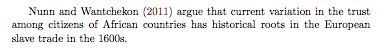
\includegraphics{./images/biblatex_inline.png}

in whatever citation style (APSA, APA, Chicago) you pre-specified!

Also at the end of your paper you will have a bibliography with entries
ordered and formatted in the appropriate citation.


\includegraphics{./images/biblatex_bibliography.png}

This is a much less frustrating way of keeping track of your references
-- no need to hand-edit formatting the bibliography to conform to
citation rules (which biblatex already knows) and no need to update your
bibliography as you add and drop references (biblatex will only show
entries that are used in the main text).

\hypertarget{stocking-up-on-your-.bib-files}{%
\subsection{stocking up on your .bib
files}\label{stocking-up-on-your-.bib-files}}

You should keep your own \texttt{.bib} file that has all your
bibliographical resources. Storing entries is cheap (does not take much
memory), so it is fine to keep all your references in one place (but
you'll want to make a new one for collaborative projects where multiple
people will compile a \texttt{.tex} file).

For example, Gary's BibTeX file is here:
\url{https://github.com/iqss-research/gkbibtex/blob/master/gk.bib}

Citation management software (Mendeley or Zotero) automatically
generates .bib entries from your library of PDFs for you, provided you
have the bibliography attributes right.

\hypertarget{extension-optional-exercise}{%
\section*{Extension: Optional
Exercise}\label{extension-optional-exercise}}
\addcontentsline{toc}{section}{Extension: Optional Exercise}

Create a LaTeX document for a hypothetical research paper on your laptop
and, once you've verified it compiles into a PDF, come show it to either
one of the instructors.

You can also use overleaf if you have preference for a cloud-based
system. But don't swallow the built-in templates without understanding
or testing them.

Each student will have slightly different substantive interests, so we
won't impose much of a standard. But at a minimum, the LaTeX document
should have:

\begin{itemize}
\tightlist
\item
  A title, author, date, and abstract
\item
  Sections
\item
  Italics and boldface
\item
  A figure with a caption and in-text reference to it.
\end{itemize}

Depending on your subfield or interests, try to implement some of the
following:

\begin{itemize}
\tightlist
\item
  A bibliographical reference drawing from a separate \texttt{.bib} file
\item
  A table
\item
  A math expression
\item
  A different font
\item
  Different page margins
\item
  Different line spacing
\end{itemize}

\part{II Linear Algebra}

\hypertarget{linearalgebra}{%
\chapter{Linear Algebra}\label{linearalgebra}}

\hypertarget{vector-def}{%
\section{Working with Vectors}\label{vector-def}}

\textbf{Vector}: A vector in \(n\)-space is an ordered list of \(n\)
numbers. These numbers can be represented as either a row vector or a
column vector:

\[{\bf v} = \begin{bmatrix} v_1 & v_2 & \dots & v_n\end{bmatrix}\]

\[{\bf v} = \begin{bmatrix} v_1 \\ v_2 \\ \vdots \\ v_n \end{bmatrix}\]

We can also think of a vector as defining a point in \(n\)-dimensional
space, usually \(\mathbb{R}^n\); each element of the vector defines the
coordinate of the point in a particular direction.

\textbf{Vector Addition and Subtraction}: If two vectors, \({\bf u}\)
and \({\bf v}\), have the same length (i.e.~have the same number of
elements), they can be added (subtracted) together:

\[{\bf u} + {\bf v} = \begin{bmatrix} u_1 + v_1 \\ u_2 + v_2 \\ \vdots \\ u_k + v_n \end{bmatrix}\]

\[{\bf u} - {\bf v} = \begin{bmatrix} u_1 - v_1 \\ u_2 - v_2 \\ \vdots \\ u_k - v_n \end{bmatrix}\]

\textbf{Scalar Multiplication}: The product of a scalar \(c\) (i.e.~a
constant) and vector \({\bf v}\) is:\\

\[ c{\bf v} =  \begin{bmatrix} cv_1 \\ cv_2 \\ \dots \\ cv_n \end{bmatrix} \]

\textbf{Vector Inner Product}: The inner product (also called the dot
product or scalar product) of two vectors \({\bf u}\) and \({\bf v}\) is
again defined if and only if they have the same number of elements

\[ {\bf u} \cdot {\bf v} = u_1v_1 + u_2v_2 + \cdots + u_nv_n = \sum_{i = 1}^n u_iv_i\]

If \({\bf u} \cdot {\bf v} = 0\), the two vectors are orthogonal (or
perpendicular).

\textbf{Vector Norm}: The norm of a vector is a measure of its length.
There are many different ways to calculate the norm, but the most common
is the Euclidean norm (which corresponds to our usual conception of
distance in three-dimensional space):

\[ ||{\bf v}|| = \sqrt{{\bf v}\cdot{\bf v}} = \sqrt{ v_1v_1 + v_2v_2 + \cdots + v_nv_n}\]

\leavevmode\vadjust pre{\hypertarget{exm-vectors}{}}%
\begin{example}[]\label{exm-vectors}

Let \(a = \begin{bmatrix} 2\\1\\2\end{bmatrix}\),
\(b = \begin{bmatrix} 3\\4\\5 \end{bmatrix}\). Calculate the following:

\begin{enumerate}
\def\labelenumi{\arabic{enumi}.}
\tightlist
\item
  \(a - b\)
\item
  \(a \cdot b\)
\end{enumerate}

\end{example}

\leavevmode\vadjust pre{\hypertarget{exr-vectors1}{}}%
\begin{exercise}[]\label{exr-vectors1}

Let \(u = \begin{bmatrix} 7\\1\\-5\\3\end{bmatrix}\),
\(v = \begin{bmatrix} 9\\-3\\2\\8 \end{bmatrix}\),
\(w = \begin{bmatrix} 1\\13\\ -7\\2 \\15 \end{bmatrix}\), and \(c = 2\).
Calculate the following:

\begin{enumerate}
\def\labelenumi{\arabic{enumi}.}
\item
  \(u-v\)
\item
  \(cw\)
\item
  \(u \cdot v\)
\item
  \(w \cdot v\)
\end{enumerate}

\end{exercise}

\hypertarget{linearindependence}{%
\section{Linear Independence}\label{linearindependence}}

\textbf{Linear combinations}: The vector \({\bf u}\) is a linear
combination of the vectors \({\bf v}_1, {\bf v}_2, \cdots , {\bf v}_k\)
if

\[{\bf u} = c_1{\bf v}_1 + c_2{\bf v}_2 +  \cdots + c_k{\bf v}_k\]

For example, \(\begin{bmatrix}9 \\ 13 \\ 17 \end{bmatrix}\) is a linear
combination of the following three vectors:
\(\begin{bmatrix}1 \\ 2 \\ 3 \end{bmatrix}\),
\(\begin{bmatrix} 2 \\ 3\\ 4\end{bmatrix}\), and
\(\begin{bmatrix} 3 \\ 4 \\ 5 \end{bmatrix}\). This is because
\(\begin{bmatrix}9 \\ 13 \\ 17 \end{bmatrix}\) =
\((2)\begin{bmatrix}1 \\ 2 \\ 3 \end{bmatrix}\)
\(+ (-1)\begin{bmatrix} 2 \\ 3\\ 4\end{bmatrix}\) +
\(3\begin{bmatrix} 3 \\ 4 \\ 5 \end{bmatrix}\)

\textbf{Linear independence}: A set of vectors
\({\bf v}_1, {\bf v}_2, \cdots , {\bf v}_k\) is linearly independent if
the only solution to the equation

\[c_1{\bf v}_1 + c_2{\bf v}_2 +  \cdots + c_k{\bf v}_k = 0\]

is \(c_1 = c_2 = \cdots = c_k = 0\). If another solution exists, the set
of vectors is linearly dependent.

A set \(S\) of vectors is linearly dependent if and only if at least one
of the vectors in \(S\) can be written as a linear combination of the
other vectors in \(S\).

Linear independence is only defined for sets of vectors with the same
number of elements; any linearly independent set of vectors in
\(n\)-space contains at most \(n\) vectors.

Since \(\begin{bmatrix}9 \\ 13 \\ 17 \end{bmatrix}\) is a linear
combination of \(\begin{bmatrix}1 \\ 2 \\ 3 \end{bmatrix}\),
\(\begin{bmatrix} 2 \\ 3\\ 4\end{bmatrix}\), and
\(\begin{bmatrix} 3 \\ 4 \\ 5 \end{bmatrix}\), these 4 vectors
constitute a linearly dependent set.

\leavevmode\vadjust pre{\hypertarget{exm-linearindep}{}}%
\begin{example}[]\label{exm-linearindep}

Are the following sets of vectors linearly independent?

\begin{enumerate}
\def\labelenumi{\arabic{enumi}.}
\tightlist
\item
  \(\begin{bmatrix}2 \\ 3 \\ 1 \end{bmatrix}\) and
  \(\begin{bmatrix}4 \\ 6 \\ 1 \end{bmatrix}\)
\item
  \(\begin{bmatrix}1 \\ 0 \\ 0 \end{bmatrix}\),
  \(\begin{bmatrix}0 \\ 5 \\ 0 \end{bmatrix}\), and
  \(\begin{bmatrix}10 \\ 10 \\ 0 \end{bmatrix}\)
\end{enumerate}

\end{example}

\leavevmode\vadjust pre{\hypertarget{exr-linearindep1}{}}%
\begin{exercise}[]\label{exr-linearindep1}

Are the following sets of vectors linearly independent?

\begin{enumerate}
\def\labelenumi{\arabic{enumi}.}
\item
  \[{\bf v}_1 = \begin{bmatrix} 1 \\ 0 \\ 0 \end{bmatrix} , {\bf v}_2 = \begin{bmatrix} 1 \\ 0 \\ 1 \end{bmatrix} , {\bf v}_3 = \begin{bmatrix} 1 \\ 1 \\ 1 \end{bmatrix} \]
\item
  \[{\bf v}_1 = \begin{bmatrix} 2 \\ 2 \\ 1 \end{bmatrix} , {\bf v}_2 = \begin{bmatrix} -4 \\ 6 \\ 5 \end{bmatrix} , {\bf v}_3 = \begin{bmatrix} -2 \\ 8 \\ 6 \end{bmatrix} \]
\end{enumerate}

\end{exercise}

\hypertarget{matrixbasics}{%
\section{Basics of Matrix Algebra}\label{matrixbasics}}

\textbf{Matrix}: A matrix is an array of real numbers arranged in \(m\)
rows by \(n\) columns. The dimensionality of the matrix is defined as
the number of rows by the number of columns, \(m \times n\).

\[{\bf A}=\begin{bmatrix}
    a_{11} & a_{12} & \cdots & a_{1n} \\
    a_{21} & a_{22} & \cdots & a_{2n} \\
    \vdots & \vdots & \ddots & \vdots \\
    a_{m1} & a_{m2} & \cdots & a_{mn}
\end{bmatrix}\]

Note that you can think of vectors as special cases of matrices; a
column vector of length \(k\) is a \(k \times 1\) matrix, while a row
vector of the same length is a \(1 \times k\) matrix.

It's also useful to think of matrices as being made up of a collection
of row or column vectors. For example,

\[\bf A = \begin{bmatrix} {\bf a}_1 & {\bf a}_2 &  \cdots & {\bf a}_m \end{bmatrix}\]

\textbf{Matrix Addition}: Let \(\bf A\) and \(\bf B\) be two
\(m\times n\) matrices.

\[\mathbf{A+B}=\begin{bmatrix} a_{11}+b_{11} & a_{12}+b_{12} & \cdots & a_{1n}+b_{1n} \\ a_{21}+b_{21} & a_{22}+b_{22} & \cdots & a_{2n}+b_{2n} \\ \vdots & \vdots  & \ddots & \vdots \\ a_{m1}+b_{m1} & a_{m2}+b_{m2} & \cdots & a_{mn}+b_{mn} \end{bmatrix}\]

Note that matrices \({\bf A}\) and \({\bf B}\) must have the same
dimensionality, in which case they are \textbf{conformable for
addition}.

\leavevmode\vadjust pre{\hypertarget{exm-matrixaddition}{}}%
\begin{example}[]\label{exm-matrixaddition}

\[{\bf A}=\begin{bmatrix} 1 & 2 & 3 \\ 4 & 5 & 6 \end{bmatrix}, \qquad {\bf B}=\begin{bmatrix} 1 & 2 & 1 \\ 2 & 1 & 2 \end{bmatrix}\]

Find \(\mathbf{A}+\mathbf{B}\)

\end{example}

\textbf{Scalar Multiplication}: Given the scalar \(s\), the scalar
multiplication of \(s {\bf A}\) is

\[ s {\bf A}=  s \begin{bmatrix} a_{11} & a_{12} & \cdots & a_{1n} \\ a_{21} & a_{22} & \cdots & a_{2n} \\ \vdots & \vdots & \ddots & \vdots \\ a_{m1} & a_{m2} & \cdots & a_{mn} \end{bmatrix} = \begin{bmatrix} s a_{11} & s a_{12} & \cdots & s a_{1n} \\ s a_{21} & s a_{22} & \cdots & s a_{2n} \\ \vdots & \vdots & \ddots & \vdots \\ s a_{m1} & s a_{m2} & \cdots & s a_{mn} \end{bmatrix}\]

\leavevmode\vadjust pre{\hypertarget{exm-scalarmulti}{}}%
\begin{example}[]\label{exm-scalarmulti}

\(s=2\),

\[{\bf A}=\begin{bmatrix} 1 & 2 & 3 \\ 4 & 5 & 6 \end{bmatrix}\]

Find \(s {\bf A}\)

\end{example}

\textbf{Matrix Multiplication}: If \({\bf A}\) is an \(m\times k\)
matrix and \(\bf B\) is a \(k\times n\) matrix, then their product
\(\bf C = A B\) is the \(m\times n\) matrix where

\[c_{ij}=a_{i1}b_{1j}+a_{i2}b_{2j}+\cdots+a_{ik}b_{kj}\]

\leavevmode\vadjust pre{\hypertarget{exm-matrixmulti}{}}%
\begin{example}[]\label{exm-matrixmulti}

\begin{enumerate}
\def\labelenumi{\arabic{enumi}.}
\item
  Find
  \(\begin{bmatrix} a&b\\c&d\\e&f \end{bmatrix} \begin{bmatrix} A&B\\C&D \end{bmatrix}\)
\item
  Find
  \(\begin{bmatrix} 1&2&-1\\3&1&4 \end{bmatrix} \begin{bmatrix} -2&5\\4&-3\\2&1\end{bmatrix}\)
\end{enumerate}

\end{example}

Note that the number of columns of the first matrix must equal the
number of rows of the second matrix, in which case they are
\textbf{conformable for multiplication}. The sizes of the matrices
(including the resulting product) must be
\[(m\times k)(k\times n)=(m\times n)\]

Also note that if \textbf{AB} exists, \textbf{BA} exists only if
\(\dim({\bf A}) = m \times n\) and \(\dim({\bf B}) = n \times m\).

This does not mean that \textbf{AB} = \textbf{BA}. \textbf{AB} =
\textbf{BA} is true only in special circumstances, like when \({\bf A}\)
or \({\bf B}\) is an identity matrix or \({\bf A} = {\bf B}^{-1}\).

\hypertarget{laws-of-matrix-algebra}{%
\subsection{Laws of Matrix Algebra}\label{laws-of-matrix-algebra}}

\begin{enumerate}
\def\labelenumi{\arabic{enumi}.}
\tightlist
\item
  Associative: \(\bf (A+B)+C = A+(B+C)\)
\item
  \(\bf (AB)C = A(BC)\)
\item
  Commutative: \(\bf A+B=B+A\)
\item
  Distributive: \(\bf A(B+C)=AB+AC\)
\item
  \(\bf (A+B)C=AC+BC\)
\end{enumerate}

Commutative law for multiplication does not hold -- the order of
multiplication matters:

\[\bf AB \ne BA\]

For example,

\[{\bf A}=\begin{bmatrix} 1&2\\-1&3\end{bmatrix}, \qquad {\bf B}=\begin{bmatrix} 2&1\\0&1\end{bmatrix}\]

\[{\bf AB}=\begin{bmatrix} 2&3\\-2&2\end{bmatrix}, \qquad {\bf BA}=\begin{bmatrix} 1&7\\-1&3\end{bmatrix}\]

\textbf{Transpose}: The transpose of the \(m\times n\) matrix \(\bf A\)
is the \(n\times m\) matrix \({\bf A}^\top\) (also written \({\bf A}'\))
obtained by interchanging the rows and columns of \(\bf A\).

For example,

\({\bf A}=\begin{bmatrix} 4&-2&3\\0&5&-1\end{bmatrix}, \qquad {\bf A}^\top=\begin{bmatrix} 4&0\\-2&5\\3&-1 \end{bmatrix}\)

\({\bf B}=\begin{bmatrix} 2\\-1\\3 \end{bmatrix}, \qquad {\bf B}^\top=\begin{bmatrix} 2&-1&3\end{bmatrix}\)

The following rules apply for transposed matrices:

\begin{enumerate}
\def\labelenumi{\arabic{enumi}.}
\tightlist
\item
  \(({\bf A+B})^\top = {\bf A}^\top+{\bf B}^\top\)
\item
  \(({\bf A}^\top)^\top={\bf A}\)
\item
  \((s{\bf A})^\top = s{\bf A}^\top\)
\item
  \(({\bf AB})^\top = {\bf B}^\top{\bf A}^\top\); and by induction
  \(({\bf ABC})^\top = {\bf C}^\top{\bf B}^\top{\bf A}^\top\)
\end{enumerate}

Example of \(({\bf AB})^\top = {\bf B}^\top{\bf A}^\top\):

\[{\bf A}=\begin{bmatrix} 1&3&2\\2&-1&3\end{bmatrix}, \qquad {\bf B}=\begin{bmatrix} 0&1\\2&2\\3&-1\end{bmatrix}\]

\[ ({\bf AB})^\top = \left[ \begin{bmatrix} 1&3&2\\2&-1&3\end{bmatrix} \begin{bmatrix} 0&1\\2&2\\3&-1\end{bmatrix} \right]^\top = \begin{bmatrix} 12&7\\5&-3 \end{bmatrix}\]

\[ {\bf B}^\top{\bf A}^\top= \begin{bmatrix} 0&2&3\\1&2&-1 \end{bmatrix}  \begin{bmatrix} 1&2\\3&-1\\2&3 \end{bmatrix} = \begin{bmatrix} 12&7\\5&-3 \end{bmatrix}\]

\leavevmode\vadjust pre{\hypertarget{exr-matrixmulti1}{}}%
\begin{exercise}[]\label{exr-matrixmulti1}

Let

\[A =  \begin{bmatrix} 2&0&-1&1\\1&2&0&1 \end{bmatrix}\]

\[B = \begin{bmatrix} 1&5&-7\\1&1&0\\0&-1&1\\2&0&0\end{bmatrix}\]

\[C =  \begin{bmatrix} 3&2&-1\\0&4&6 \end{bmatrix}\]

Calculate the following:

\begin{enumerate}
\def\labelenumi{\arabic{enumi}.}
\tightlist
\item
  \[AB\]
\item
  \[BA\]
\item
  \[(BC)^\top\]
\item
  \[BC^\top\]
\end{enumerate}

\end{exercise}

\hypertarget{systems-of-linear-equations}{%
\section{Systems of Linear
Equations}\label{systems-of-linear-equations}}

\hypertarget{linear-equation}{%
\subsection{Linear Equation}\label{linear-equation}}

Linear equations take form of
\(a_1 x_1 + a_2 x_2 + \cdots + a_n x_n = b\)

\(a_i\) are parameters or coefficients. \(x_i\) are variables or
unknowns.

Linear because only one variable per term and degree is at most 1.

We are often interested in solving linear systems like

\[\left\{\begin{array}{ll} x-3y &= -3\\ 2x +y &= 8 \end{array}\right.\]

More generally, we might have a system of \(m\) equations in \(n\)
unknowns \[\begin{matrix}
        a_{11}x_1  & + & a_{12}x_2 & + & \cdots & + & a_{1n}x_n & = & b_1\\
        a_{21}x_1  & + & a_{22}x_2 & + & \cdots & + & a_{2n}x_n & = & b_2\\
        \vdots     &   &     &   & \vdots &   &     & \vdots & \\
        a_{m1}x_1  & + & a_{m2}x_2 & + & \cdots & + & a_{mn}x_n & = & b_m
        \end{matrix}\]

A \textbf{solution} to a linear system of \(m\) equations in \(n\)
unknowns is a set of \(n\) numbers \(x_1, x_2, \cdots, x_n\) that
satisfy each of the \(m\) equations.

Example: \(x=3\) and \(y=2\) is the solution to the above \(2\times 2\)
linear system. If you graph the two lines, you will find that they
intersect at \((3,2)\).

Does a linear system have one, no, or multiple solutions? For a system
of 2 equations with 2 unknowns (i.e., two lines):

\begin{itemize}
\tightlist
\item
  \textbf{One solution:} The lines intersect at exactly one point.
\item
  \textbf{No solution:} The lines are parallel.
\item
  \textbf{Infinite solutions:} The lines coincide.
\end{itemize}

Methods to solve linear systems:

\begin{enumerate}
\def\labelenumi{\arabic{enumi}.}
\tightlist
\item
  Substitution
\item
  Elimination of variables
\item
  Matrix methods
\end{enumerate}

\leavevmode\vadjust pre{\hypertarget{exr-lineareq}{}}%
\begin{exercise}[]\label{exr-lineareq}

Provide a system of 2 equations with 2 unknowns that has

\begin{enumerate}
\def\labelenumi{\arabic{enumi}.}
\tightlist
\item
  one solution
\item
  no solution
\item
  infinite solutions
\end{enumerate}

\end{exercise}

\hypertarget{systems-of-equations-as-matrices}{%
\section{Systems of Equations as
Matrices}\label{systems-of-equations-as-matrices}}

Matrices provide an easy and efficient way to represent linear systems
such as \[\begin{matrix}
        a_{11}x_1  & + & a_{12}x_2 & + & \cdots & + & a_{1n}x_n & = & b_1\\
        a_{21}x_1  & + & a_{22}x_2 & + & \cdots & + & a_{2n}x_n & = & b_2\\
        \vdots     &   &     &   & \vdots &   &     & \vdots & \\
        a_{m1}x_1  & + & a_{m2}x_2 & + & \cdots & + & a_{mn}x_n & = & b_m
        \end{matrix}\]

as \[{\bf A x = b}\] where

The \(m \times n\) \textbf{coefficient matrix} \({\bf A}\) is an array
of \(m n\) real numbers arranged in \(m\) rows by \(n\) columns:
\[{\bf A}=\begin{bmatrix}
    a_{11} & a_{12} & \cdots & a_{1n} \\
    a_{21} & a_{22} & \cdots & a_{2n} \\
    \vdots &  & \ddots & \vdots \\
    a_{m1} & a_{m2} & \cdots & a_{mn}
    \end{bmatrix}\]

The unknown quantities are represented by the vector
\({\bf x}=\begin{bmatrix} x_1\\x_2\\\vdots\\x_n \end{bmatrix}\).

The right hand side of the linear system is represented by the vector
\({\bf b}=\begin{bmatrix} b_1\\b_2\\\vdots\\b_m \end{bmatrix}\).

\textbf{Augmented Matrix}: When we append \(\bf b\) to the coefficient
matrix \(\bf A\), we get the augmented matrix
\(\widehat{\bf A}=[\bf A | b]\) \[\begin{bmatrix}
    a_{11} & a_{12} & \cdots & a_{1n} & | & b_1\\
    a_{21} & a_{22} & \cdots & a_{2n} & | & b_2\\
    \vdots &  & \ddots & \vdots & | & \vdots\\
    a_{m1} & a_{m2} & \cdots & a_{mn} & | & b_m
    \end{bmatrix}\]

\leavevmode\vadjust pre{\hypertarget{exr-augmatrix}{}}%
\begin{exercise}[]\label{exr-augmatrix}

Create an augmented matrix that represent the following system of
equations:

\[2x_1 -7x_2 + 9x_3 -4x_4 = 8\]

\[41x_2 + 9x_3 -5x_6 = 11\]

\[x_1 -15x_2 -11x_5 = 9\]

\end{exercise}

\hypertarget{finding-solutions-to-augmented-matrices-and-systems-of-equations}{%
\section{Finding Solutions to Augmented Matrices and Systems of
Equations}\label{finding-solutions-to-augmented-matrices-and-systems-of-equations}}

\textbf{Row Echelon Form}: Our goal is to translate our augmented matrix
or system of equations into row echelon form. This will provide us with
the values of the vector \textbf{x} which solve the system. We use the
row operations to change coefficients in the lower triangle of the
augmented matrix to 0. An augmented matrix of the form \[\begin{bmatrix}
    \fbox{$a'_{11}$}& a'_{12} & a'_{13}& \cdots & a'_{1n} & | & b'_1\\
    0 & \fbox{$a'_{22}$} & a'_{23}& \cdots & a'_{2n} & | & b'_2\\
    0 & 0 & \fbox{$a'_{33}$}& \cdots & a'_{3n} & | & b'_3\\
    0 & 0 &0 & \ddots & \vdots  & | & \vdots \\
    0 & 0 &0 &0 & \fbox{$a'_{mn}$} & | & b'_m
    \end{bmatrix}\]

is said to be in row echelon form --- each row has more leading zeros
than the row preceding it.

\textbf{Reduced Row Echelon Form}: We can go one step further and put
the matrix into reduced row echelon form. Reduced row echelon form makes
the value of \textbf{x} which solves the system very obvious. For a
system of \(m\) equations in \(m\) unknowns, with no all-zero rows, the
reduced row echelon form would be

\[\begin{bmatrix}
    \fbox{$1$}  &  0 &   0 &    0  &   0 & | & b^*_1\\
    0  &  \fbox{$1$} &   0 &    0  &   0 & | & b^*_2\\
    0  &  0 &   \fbox{$1$} &    0  &   0 & | & b^*_3\\
    0  &  0 &   0 &\ddots &   0 & | &\vdots\\
    0  &  0 &   0 &    0  &   \fbox{$1$} & | & b^*_m
    \end{bmatrix}\]

\textbf{Gaussian and Gauss-Jordan elimination}: We can conduct
elementary row operations to get our augmented matrix into row echelon
or reduced row echelon form. The methods of transforming a matrix or
system into row echelon and reduced row echelon form are referred to as
Gaussian elimination and Gauss-Jordan elimination, respectively.

\textbf{Elementary Row Operations}: To do Gaussian and Gauss-Jordan
elimination, we use three basic operations to transform the augmented
matrix into another augmented matrix that represents an equivalent
linear system -- equivalent in the sense that the same values of \(x_j\)
solve both the original and transformed matrix/system:

\textbf{Interchanging Rows}: Suppose we have the augmented matrix
\[{\widehat{\bf A}}=\begin{bmatrix} a_{11} & a_{12} & | & b_1\\
        a_{21} & a_{22} & | & b_2 
        \end{bmatrix}\] If we interchange the two rows, we get the
augmented matrix \[\begin{bmatrix}
        a_{21} & a_{22} & | & b_2\\
        a_{11} & a_{12} & | & b_1
        \end{bmatrix}\] which represents a linear system equivalent to
that represented by matrix \(\widehat{\bf A}\).

\textbf{Multiplying by a Constant}: If we multiply the second row of
matrix \(\widehat{\bf A}\) by a constant \(c\), we get the augmented
matrix \[\begin{bmatrix}
        a_{11} & a_{12} & | & b_1\\
        c a_{21} & c a_{22} & | & c b_2
        \end{bmatrix}\] which represents a linear system equivalent to
that represented by matrix \(\widehat{\bf A}\).

\textbf{Adding (subtracting) Rows}: If we add (subtract) the first row
of matrix \(\widehat{\bf A}\) to the second, we obtain the augmented
matrix \[\begin{bmatrix}
        a_{11} & a_{12} & | & b_1\\
        a_{11}+a_{21} & a_{12}+a_{22} & | & b_1+b_2
        \end{bmatrix}\] which represents a linear system equivalent to
that represented by matrix \(\widehat{\bf A}\).

\leavevmode\vadjust pre{\hypertarget{exm-solvesys}{}}%
\begin{example}[]\label{exm-solvesys}

Solve the following system of equations by using elementary row
operations: \[\begin{matrix}
    x  & - & 3y & = & -3\\
    2x & + &  y & = &  8
    \end{matrix}\]

\end{example}

\leavevmode\vadjust pre{\hypertarget{exr-solvesys1}{}}%
\begin{exercise}[]\label{exr-solvesys1}

Put the following system of equations into augmented matrix form. Then,
using Gaussian or Gauss-Jordan elimination, solve the system of
equations by putting the matrix into row echelon or reduced row echelon
form.

\begin{enumerate}
\def\labelenumi{\arabic{enumi}.}
\tightlist
\item
  \[ \begin{cases}
      x + y + 2z = 2\\
      3x - 2y + z = 1\\
      y - z = 3
   \end{cases}\]
\item
  \[ \begin{cases}
      2x + 3y - z = -8\\
      x + 2y - z = 12\\
    -x -4y + z = -6
   \end{cases}\]
\end{enumerate}

\end{exercise}

\hypertarget{rank-of-a-matrix}{%
\section{Rank of a Matrix}\label{rank-of-a-matrix}}

To determine how many solutions exist, we can use information about (1)
the number of equations \(m\), (2) the number of unknowns \(n\), and (3)
the \textbf{rank} of the matrix representing the linear system.

\textbf{Rank}: The maximum number of linearly independent row or column
vectors in the matrix. This is equivalent to the number of nonzero rows
of a matrix in row echelon form. For any matrix \textbf{A}, the row rank
always equals column rank, and we refer to this number as the rank of
\textbf{A}.

For example \[\begin{bmatrix} 1 & 2 & 3 \\
            0 & 4 & 5 \\
            0 & 0 & 6 \end{bmatrix}\]

Rank = 3

\[\begin{bmatrix} 1 & 2 & 3 \\ 
    0 & 4 & 5 \\
    0 & 0 & 0 \end{bmatrix}\]

Rank = 2

\leavevmode\vadjust pre{\hypertarget{exr-rank}{}}%
\begin{exercise}[]\label{exr-rank}

Find the rank of each matrix below:

(Hint: transform the matrices into row echelon form. Remember that the
number of nonzero rows of a matrix in row echelon form is the rank of
that matrix)

\begin{enumerate}
\def\labelenumi{\arabic{enumi}.}
\item
  \[\begin{bmatrix} 1 & 1 & 2 \\ 
    2 & 1 & 3 \\
    1 & 2 & 3 \end{bmatrix}\]
\item
  \[\begin{bmatrix} 1 & 3 & 3 & -3 & 3\\ 
  1 & 3 & 1 & 1 & 3 \\
  1 & 3 & 2 & -1 & -2 \\
  1 & 3 & 0 & 3 & -2 \end{bmatrix}\]
\end{enumerate}

\end{exercise}

Answer to Exercise~\ref{exr-rank}:

\begin{enumerate}
\def\labelenumi{\arabic{enumi}.}
\tightlist
\item
  rank is 2
\item
  rank is 3
\end{enumerate}

\hypertarget{the-inverse-of-a-matrix}{%
\section{The Inverse of a Matrix}\label{the-inverse-of-a-matrix}}

\textbf{Identity Matrix}: The \(n\times n\) identity matrix
\({\bf I}_n\) is the matrix whose diagonal elements are 1 and all
off-diagonal elements are 0. Examples:
\[ {\bf I}_2=\begin{bmatrix} 1&0\\0&1 \end{bmatrix}, \qquad {\bf I}_3=\begin{bmatrix} 1&0&0\\ 0&1&0\\ 
            0&0&1 \end{bmatrix}\]

\textbf{Inverse Matrix}: An \(n\times n\) matrix \({\bf A}\) is
\textbf{nonsingular} or \textbf{invertible} if there exists an
\(n\times n\) matrix \({\bf A}^{-1}\) such that
\[{\bf A} {\bf A}^{-1} = {\bf A}^{-1} {\bf A} = {\bf I}_n\] where
\({\bf A}^{-1}\) is the inverse of \({\bf A}\). If there is no such
\({\bf A}^{-1}\), then \({\bf A}\) is singular or not invertible.

Example: Let
\[{\bf A} = \begin{bmatrix} 2&3\\2&2 \end{bmatrix}, \qquad {\bf B}=\begin{bmatrix} -1&\frac{3}{2}\\ 1&-1
        \end{bmatrix}\] Since
\[{\bf A} {\bf B} = {\bf B} {\bf A} = {\bf I}_n\] we conclude that
\({\bf B}\) is the inverse, \({\bf A}^{-1}\), of \({\bf A}\) and that
\({\bf A}\) is nonsingular.

\textbf{Properties of the Inverse}:

\begin{itemize}
\item
  If the inverse exists, it is unique.
\item
  If \({\bf A}\) is nonsingular, then \({\bf A}^{-1}\) is nonsingular.
\item
  \(({\bf A}^{-1})^{-1} = {\bf A}\)
\item
  If \({\bf A}\) and \({\bf B}\) are nonsingular, then
  \({\bf A}{\bf B}\) is nonsingular
\item
  \(({\bf A}{\bf B})^{-1} = {\bf B}^{-1}{\bf A}^{-1}\)
\item
  If \({\bf A}\) is nonsingular, then
  \(({\bf A}^\top)^{-1}=({\bf A}^{-1})^\top\)
\end{itemize}

\textbf{Procedure to Find} \({\bf A}^{-1}\): We know that if \({\bf B}\)
is the inverse of \({\bf A}\), then
\[{\bf A} {\bf B} = {\bf B} {\bf A} = {\bf I}_n\] Looking only at the
first and last parts of this \[{\bf A} {\bf B} = {\bf I}_n\] Solving for
\({\bf B}\) is equivalent to solving for \(n\) linear systems, where
each column of \({\bf B}\) is solved for the corresponding column in
\({\bf I}_n\). We can solve the systems simultaneously by augmenting
\({\bf A}\) with \({\bf I}_n\) and performing Gauss-Jordan elimination
on \({\bf A}\). If Gauss-Jordan elimination on \([{\bf A} | {\bf I}_n]\)
results in \([{\bf I}_n | {\bf B} ]\), then \({\bf B}\) is the inverse
of \({\bf A}\). Otherwise, \({\bf A}\) is singular.

To summarize: To calculate the inverse of \({\bf A}\)

\begin{enumerate}
\def\labelenumi{\arabic{enumi}.}
\item
  Form the augmented matrix \([ {\bf A} | {\bf I}_n]\)
\item
  Using elementary row operations, transform the augmented matrix to
  reduced row echelon form.
\item
  The result of step 2 is an augmented matrix \([ {\bf C} | {\bf B} ]\).

  \begin{enumerate}
  \def\labelenumii{\alph{enumii}.}
  \item
    If \({\bf C}={\bf I}_n\), then \({\bf B}={\bf A}^{-1}\).
  \item
    If \({\bf C}\ne{\bf I}_n\), then \(\bf C\) has a row of zeros. This
    means \({\bf A}\) is singular and \({\bf A}^{-1}\) does not exist.
  \end{enumerate}
\end{enumerate}

\leavevmode\vadjust pre{\hypertarget{exm-inverse}{}}%
\begin{example}[]\label{exm-inverse}

Find the inverse of the following matrix:

\[{\bf A}=\begin{bmatrix} 1&1&1\\0&2&3\\5&5&1 \end{bmatrix}\]

\end{example}

\leavevmode\vadjust pre{\hypertarget{exr-inverse1}{}}%
\begin{exercise}[]\label{exr-inverse1}

Find the inverse of the following matrix:

\[{\bf A}=\begin{bmatrix} 1&0&4\\0&2&0\\0&0&1 \end{bmatrix}\]

\end{exercise}

\hypertarget{linear-systems-and-inverses}{%
\section{Linear Systems and
Inverses}\label{linear-systems-and-inverses}}

Let's return to the matrix representation of a linear system

\[\bf{Ax} = \bf{b}\]

If \(\bf{A}\) is an \(n\times n\) matrix,then \(\bf{Ax}=\bf{b}\) is a
system of \(n\) equations in \(n\) unknowns. Suppose \(\bf{A}\) is
nonsingular. Then \(\bf{A}^{-1}\) exists. To solve this system, we can
multiply each side by \(\bf{A}^{-1}\) and reduce it as follows:

\[\begin{align*} \bf{A}^{-1} (\bf{A} \bf{x}) & =  \bf{A}^{-1} \bf{b} \\ (\bf{A}^{-1} \bf{A})\bf{x} & =  \bf{A}^{-1} \bf{b}\\ \bf{I}_n \bf{x}     & =  \bf{A}^{-1} \bf{b}\\ \bf{x} & =  \bf{A}^{-1} \bf{b} \end{align*} \]

Hence, given \(\bf{A}\) and \(\bf{b}\) and given that \(\bf{A}\) is
nonsingular, then \(\bf{x} = \bf{A}^{-1} \bf{b}\) is a unique solution
to this system.

\leavevmode\vadjust pre{\hypertarget{exr-invlinsys}{}}%
\begin{exercise}[]\label{exr-invlinsys}

Use the inverse matrix to solve the following linear system:

\[ \begin{align*} 
  -3x + 4y &= 5 \\
  2x - y &= -10
  \end{align*} \]

\textbf{Hint}: the linear system above can be written in the matrix form

\(\textbf{A}\textbf{z} = \textbf{b}\)

given

\[\textbf{A} = \begin{bmatrix} -3&4\\2&-1 \end{bmatrix},\]

\[\textbf{z} = \begin{bmatrix} x\\y \end{bmatrix},\]

and

\[\textbf{b} = \begin{bmatrix} 5\\-10 \end{bmatrix}\]

\end{exercise}

\hypertarget{determinants}{%
\section{Determinants}\label{determinants}}

\textbf{Singularity}: Determinants can be used to determine whether a
square matrix is nonsingular.

A square matrix is nonsingular if and only if its determinant is not
zero.

Determinant of a \(1 \times 1\) matrix, equals
\(|\mathbf{A}|=|a_{11}|=a_{11}\)

Determinant of a \(2 \times 2\) matrix,

\[\mathbf{A}=\begin{vmatrix} a_{11}&a_{12}\\ a_{21}&a_{22} \end{vmatrix}\]

\[\begin{align*}\det({\bf A}) &= |{\bf A}|\\
            &= a_{11}|a_{22}| - a_{12}|a_{21}|\\
            &= a_{11}a_{22} - a_{12}a_{21}
  \end{align*}\]

We can extend the second to last equation above to get the definition of
the determinant of a \(3 \times 3\) matrix: \[\begin{align*}
            \begin{vmatrix} a_{11}&a_{12}&a_{13}\\  a_{21} & a_{22}&a_{23}\\ a_{31}&a_{32}&a_{33} \end{vmatrix} 
                &= 
                a_{11} \begin{vmatrix} a_{22}&a_{23}\\ a_{32}&a_{33} \end{vmatrix}
                - a_{12} \begin{vmatrix} a_{21}&a_{23}\\ a_{31}&a_{33} \end{vmatrix}
                + a_{13} \begin{vmatrix} a_{21}&a_{22}\\ a_{31}&a_{32} 
                \end{vmatrix}\\
                &= a_{11}(a_{22}a_{33} - a_{23}a_{32}) - a_{12}(a_{21}a_{33} - a_{23}a_{31}) + a_{13}(a_{21}a_{32} - a_{22}a_{31})
  \end{align*} \]

Let's extend this now to any \(n\times n\) matrix. Let's define
\(\mathbf{A}_{ij}\) as the \((n-1)\times (n-1)\) submatrix of
\(\mathbf{A}\) obtained by deleting row \(i\) and column \(j\). Let the
\((i,j)\)th \textbf{minor} of \(\mathbf{A}\) be the determinant of
\(\mathbf{A}_{ij}\):

\[M_{ij} = \left|\mathbf{A}_{ij}\right|\]

Then for any \(n\times n\) matrix \(\mathbf{A}\)

\[|\mathbf{A}| = a_{11}M_{11} - a_{12}M_{12} + \cdots + (-1)^{n+1} a_{1n} M_{1n}\]

For example, in figuring out whether the following matrix has an
inverse?

\[\mathbf{A}=\begin{bmatrix} 1&1&1\\0&2&3\\5&5&1 \end{bmatrix}\]

\begin{enumerate}
\def\labelenumi{\arabic{enumi}.}
\item
  Calculate its determinant. \[\begin{align*}
   |\mathbf{A}| &= 1(2-15) - 1(0-15) + 1(0-10) \nonumber\\
   &= -13+15-10 \nonumber\\
   &= -8\nonumber
   \end{align*}\]
\item
  Since \(|{\bf A}|\ne 0\), we conclude that \({\bf A}\) has an inverse.
\end{enumerate}

\leavevmode\vadjust pre{\hypertarget{exr-determinants}{}}%
\begin{exercise}[]\label{exr-determinants}

Determine whether the following matrices are nonsingular:

\begin{enumerate}
\def\labelenumi{\arabic{enumi}.}
\item
  \[\begin{bmatrix}
    1 & 0 & 1\\
    2 & 1 & 2\\
    1 & 0 & -1
    \end{bmatrix}\]
\item
  \[\begin{bmatrix}
       2 & 1 & 2\\
       1 & 0 & 1\\
       4 & 1 & 4
   \end{bmatrix}\]
\end{enumerate}

\end{exercise}

\hypertarget{getting-inverse-of-a-matrix-using-its-determinant}{%
\section{Getting Inverse of a Matrix using its
Determinant}\label{getting-inverse-of-a-matrix-using-its-determinant}}

Thus far, we have a number of algorithms to

\begin{enumerate}
\def\labelenumi{\arabic{enumi}.}
\tightlist
\item
  Find the solution of a linear system,
\item
  Find the inverse of a matrix
\end{enumerate}

but these remain just that --- algorithms. At this point, we have no way
of telling how the solutions \(x_j\) change as the parameters \(a_{ij}\)
and \(b_i\) change, except by changing the values and ``rerunning'' the
algorithms.

With determinants, we can provide an explicit formula for the inverse
and therefore provide an explicit formula for the solution of an
\(n\times n\) linear system.

Hence, we can examine how changes in the parameters and \(b_i\) affect
the solutions \(x_j\).

\textbf{Determinant Formula for the Inverse of a \(2 \times 2\)}:

The determinant of a \(2 \times 2\) matrix
\(\mathbf{A}=\begin{bmatrix} a & b\\ c & d\\ \end{bmatrix}\) is defined
as: \[\frac{1}{\det({\bf A})} \begin{bmatrix}
            d & -b\\
            -c & a\\
        \end{bmatrix}\]

For example, Let's calculate the inverse of matrix A from
Exercise~\ref{exr-invlinsys} using the determinant formula.

Recall,

\[\mathbf{A} = \begin{bmatrix}
            -3 & 4\\
            2 & -1\\
        \end{bmatrix}\]

\[\det(\mathbf{A}) = (-3)(-1) - (4)(2) = 3 - 8  = -5\]

\[\frac{1}{\det(\mathbf{A})} \begin{bmatrix}
            -1 & -4\\
            -2 & -3\\
        \end{bmatrix}\]

\[\frac{1}{-5} \begin{bmatrix}
            -1 & -4\\
            -2 & -3\\
        \end{bmatrix}\]

\[\begin{bmatrix}
            \frac{1}{5} & \frac{4}{5}\\
            \frac{2}{5} & \frac{3}{5}\\
        \end{bmatrix}\]

\leavevmode\vadjust pre{\hypertarget{exr-calcinverse}{}}%
\begin{exercise}[]\label{exr-calcinverse}

Caculate the inverse of \(\mathbf{A}\) \[\mathbf{A} = \begin{bmatrix}
            3 & 5\\
            -7 & 2\\
        \end{bmatrix}\]

\end{exercise}

\hypertarget{answers-to-examples-and-exercises-1}{%
\section*{Answers to Examples and
Exercises}\label{answers-to-examples-and-exercises-1}}
\addcontentsline{toc}{section}{Answers to Examples and Exercises}

Answer to Example~\ref{exm-vectors}:

\begin{enumerate}
\def\labelenumi{\arabic{enumi}.}
\tightlist
\item
  \(\begin{bmatrix} -1 &-3&-3 \end{bmatrix}\)
\item
  6 + 4 + 10 = 20
\end{enumerate}

Answer to Exercise~\ref{exr-vectors1}:

\begin{enumerate}
\def\labelenumi{\arabic{enumi}.}
\tightlist
\item
  \(\begin{bmatrix} -2 &4&-7&-5 \end{bmatrix}\)
\item
  \(\begin{bmatrix} 2 &26&-14&4&30 \end{bmatrix}\)
\item
  63 -3 -10 + 24 = 74
\item
  undefined
\end{enumerate}

Answer to Example~\ref{exm-linearindep}:

\begin{enumerate}
\def\labelenumi{\arabic{enumi}.}
\tightlist
\item
  yes
\item
  no
\end{enumerate}

Answer to Exercise~\ref{exr-linearindep1}:

\begin{enumerate}
\def\labelenumi{\arabic{enumi}.}
\tightlist
\item
  yes
\item
  no (\(-v_1 -v_2 + v_3 = 0\))
\end{enumerate}

Answer to Example~\ref{exm-matrixaddition}:

\({\bf A+B}=\begin{bmatrix} 2 & 4 & 4 \\ 6 & 6 & 8 \end{bmatrix}\)

Answer to Example~\ref{exm-scalarmulti}:

\(s {\bf A} = \begin{bmatrix} 2 & 4 & 6 \\ 8 & 10 & 12 \end{bmatrix}\)

Answer to Example~\ref{exm-matrixmulti}:

\begin{enumerate}
\def\labelenumi{\arabic{enumi}.}
\item
  \(\begin{bmatrix} aA+bC&aB+bD\\cA+dC&cB+dD\\eA+fC&eB+fD \end{bmatrix}\)
\item
  \(\begin{bmatrix} 1(-2)+2(4)-1(2)&1(5)+2(-3)-1(1)\\  3(-2)+1(4)+4(2)&3(5)+1(-3)+4(1)\end{bmatrix} =  \begin{bmatrix} 4&-2\\6&16\end{bmatrix}\)
\end{enumerate}

Answer to Exercise~\ref{exr-matrixmulti1}:

\begin{enumerate}
\def\labelenumi{\arabic{enumi}.}
\item
  \(AB = \begin{bmatrix} 4 & 11 & -15 \\ 5 & 7 & -7 \end{bmatrix}\)
\item
  \(BA =\) undefined
\item
  \((BC)^\top =\) undefined
\item
  \(BC^\top = \begin{bmatrix} 1&5&-7\\1&1&0\\0&-1&1\\2&0&0\end{bmatrix}\begin{bmatrix} 3&0\\2&4\\-1&6 \end{bmatrix} =\begin{bmatrix}20 & -22 \\ 5 & 4 \\ -3 &2 \\6 & 0\end{bmatrix}\)
\end{enumerate}

Answer to Exercise~\ref{exr-lineareq}:

There are many answers to this. Some possible simple ones are as
follows:

\begin{enumerate}
\def\labelenumi{\arabic{enumi}.}
\item
  One solution: \[\begin{matrix}
           -x  & + & y & = & 0\\
           x & + &  y & = &  2
           \end{matrix}\]
\item
  No solution: \[\begin{matrix}
           -x  & + & y & = & 0\\
           x & - &  y & = &  2
           \end{matrix}\]
\item
  Infinite solutions: \[\begin{matrix}
           -x  & + & y & = & 0\\
           2x & - &  2y & = &  0
           \end{matrix}\]
\end{enumerate}

Answer to Exercise~\ref{exr-augmatrix}:

\(\begin{bmatrix}  2 & -7 & 9 & -4 & 0 & 0| & 8\\  0 & 41 & 9 & 0 & 0 & 5 | & 11\\  1 & -15 & 0 & 0 & -11 & 0 | & 9  \end{bmatrix}\)

Answer to Example~\ref{exm-solvesys}:

\[\begin{matrix}
    x  & - & 3y & = & -3\\
    2x & + &  y & = &  8
    \end{matrix}\]

\[\begin{matrix}
    x  & - & 3y & = & -3\\
       &   & 7y & = & 14\\          
    \end{matrix}\]

\[\begin{matrix}
    x  & - & 3y & = & -3\\
       &   & y & = & 2\\            
    \end{matrix}\]

\[\begin{matrix}
    x & = & 3\\
    y & = & 2\\         
    \end{matrix}\]

Answer to Exercise~\ref{exr-solvesys1}:

\begin{enumerate}
\def\labelenumi{\arabic{enumi}.}
\item
  x = 2, y = 2, z = -1
\item
  x = -17, y = -3, z = -35
\end{enumerate}

Answer to Exercise~\ref{exr-rank}:

\begin{enumerate}
\def\labelenumi{\arabic{enumi}.}
\item
  rank is 2
\item
  rank is 3
\end{enumerate}

Answer to Example~\ref{exm-inverse}:

\(\left(\begin{array}{ccc|ccc}  1&1&1&1&0&0\\  0&2&3&0&1&0\\  5&5&1&0&0&1 \end{array} \right)\)

\(\left(\begin{array}{ccc|ccc}  1&1&1 &1 &0&0\\  0&2&3 &0 &1&0\\  0&0&-4&-5&0&1 \end{array} \right)\)

\(\left(\begin{array}{ccc|ccc}  1&1&1&1 &0&0\\  0&2&3&0 &1&0\\  0&0&1&5/4&0&-1/4 \end{array} \right)\)

\(\left(\begin{array}{ccc|ccc}  1&1&0&-1/4 &0&1/4\\  0&2&0&-15/4&1&3/4\\  0&0&1&5/4 &0&-1/4 \end{array} \right)\)

\(\left(\begin{array}{ccc|ccc}  1&1&0&-1/4 &0 &1/4\\  0&1&0&-15/8&1/2&3/8\\  0&0&1&5/4 &0 &-1/4 \end{array} \right)\)

\(\left(\begin{array}{ccc|ccc}  1&0&0&13/8 &-1/2&-1/8\\  0&1&0&-15/8&1/2 &3/8\\  0&0&1&5/4 &0 &-1/4 \end{array} \right)\)

\({\bf A}^{-1} = \left(\begin{array}{ccc}  13/8 &-1/2&-1/8\\  -15/8&1/2 &3/8\\  5/4 &0 &-1/4 \end{array} \right)\)

Answer to Exercise~\ref{exr-inverse1}:

\begin{enumerate}
\def\labelenumi{\arabic{enumi}.}
\tightlist
\item
  \({\bf A}^{-1}=\begin{bmatrix} 1&0&-4\\0&\frac{1}{2}&0\\0&0&1 \end{bmatrix}\)
\end{enumerate}

Answer to Exercise~\ref{exr-invlinsys}:

\(\textbf{z} = \bf{A}^{-1} \bf{b} = \begin{bmatrix}  1/5 &4/5\\  2/5&3/5 \end{bmatrix} \begin{bmatrix}  5 \\  -10 \end{bmatrix}= \begin{bmatrix}  -7 \\  -4 \end{bmatrix} = \begin{bmatrix}  x \\  y \end{bmatrix}\)

Answer to Exercise~\ref{exr-determinants}:

\begin{enumerate}
\def\labelenumi{\arabic{enumi}.}
\item
  nonsingular
\item
  singular
\end{enumerate}

Answer to Exercise~\ref{exr-calcinverse}:

\(\begin{bmatrix}  \frac{2}{41} & \frac{-5}{41}\\  \frac{7}{41} & \frac{3}{41}\\  \end{bmatrix}\)

\hypertarget{rmatrices}{%
\chapter{Manipulating Vectors and Matrices}\label{rmatrices}}

\hypertarget{motivation-1}{%
\subsection*{Motivation}\label{motivation-1}}
\addcontentsline{toc}{subsection}{Motivation}

\href{https://dash.harvard.edu/bitstream/handle/1/11986331/nunn-slave-trade.pdf}{Nunn
and Wantchekon (2011)} -- ``The Slave Trade and the Origins of Mistrust
in Africa''\footnote{\href{https://dash.harvard.edu/bitstream/handle/1/11986331/nunn-slave-trade.pdf}{Nunn,
  Nathan, and Leonard Wantchekon. 2011. ``The Slave Trade and the
  Origins of Mistrust in Africa.'' American Economic Review 101(7):
  3221--52.}} -- argues that across African countries, the distrust of
co-ethnics fueled by the slave trade has had long-lasting effects on
modern day trust in these territories. They argued that the slave trade
created distrust in these societies in part because as some African
groups were employed by European traders to capture their neighbors and
bring them to the slave ships.

Nunn and Wantchekon use a variety of statistical tools to make their
case (adding controls, ordered logit, instrumental variables,
falsification tests, causal mechanisms), many of which will be covered
in future courses. In this module we will only touch on their first set
of analysis that use Ordinary Least Squares (OLS). OLS is likely the
most common application of linear algebra in the social sciences. We
will cover some linear algebra, matrix manipulation, and vector
manipulation from this data.

\hypertarget{where-are-we-where-are-we-headed-3}{%
\subsection*{Where are we? Where are we
headed?}\label{where-are-we-where-are-we-headed-3}}
\addcontentsline{toc}{subsection}{Where are we? Where are we headed?}

Up till now, you should have covered:

\begin{itemize}
\tightlist
\item
  R basic programming
\item
  Data Import
\item
  Data Visualization
\item
  R Markdown
\end{itemize}

Today we'll cover

\begin{itemize}
\tightlist
\item
  Matrices \& Dataframes in R
\item
  Manipulating variables
\item
  And other \texttt{R} tips
\end{itemize}

\hypertarget{read-data}{%
\section{Read Data}\label{read-data}}

\begin{Shaded}
\begin{Highlighting}[]
\FunctionTok{library}\NormalTok{(haven)}
\NormalTok{nunn\_full }\OtherTok{\textless{}{-}} \FunctionTok{read\_dta}\NormalTok{(}\StringTok{"data/input/Nunn\_Wantchekon\_AER\_2011.dta"}\NormalTok{)}
\end{Highlighting}
\end{Shaded}

Nunn and Wantchekon's main dataset has more than 20,000 observations.
Each observation is a respondent from the Afrobarometer survey.

\begin{Shaded}
\begin{Highlighting}[]
\FunctionTok{head}\NormalTok{(nunn\_full)}
\end{Highlighting}
\end{Shaded}

\begin{verbatim}
# A tibble: 6 x 59
  respno  ethni~1 murdo~2 isocode region distr~3 townv~4 locat~5 trust~6 trust~7
  <chr>   <chr>   <chr>   <chr>   <chr>  <chr>   <chr>     <dbl>   <dbl>   <dbl>
1 BEN0001 fon     FON     BEN     atlna~ KPOMAS~ TOKPA-~      30       3       3
2 BEN0002 fon     FON     BEN     atlna~ KPOMAS~ TOKPA-~      30       3       3
3 BEN0003 fon     FON     BEN     atlna~ OUIDAH  3ARROND      31       0       0
4 BEN0004 fon     FON     BEN     atlna~ OUIDAH  3ARROND      31       0       0
5 BEN0005 fon     FON     BEN     atlna~ OUIDAH  PAHOU        32       1       1
6 BEN0006 fon     FON     BEN     atlna~ OUIDAH  PAHOU        32       1       1
# ... with 49 more variables: intra_group_trust <dbl>, inter_group_trust <dbl>,
#   trust_local_council <dbl>, ln_export_area <dbl>, export_area <dbl>,
#   export_pop <dbl>, ln_export_pop <dbl>, age <dbl>, age2 <dbl>, male <dbl>,
#   urban_dum <dbl>, occupation <dbl>, religion <dbl>, living_conditions <dbl>,
#   education <dbl>, near_dist <dbl>, distsea <dbl>, loc_murdock_name <chr>,
#   loc_ln_export_area <dbl>, local_council_performance <dbl>,
#   council_listen <dbl>, corrupt_local_council <dbl>, ...
# i Use `colnames()` to see all variable names
\end{verbatim}

\begin{Shaded}
\begin{Highlighting}[]
\FunctionTok{colnames}\NormalTok{(nunn\_full)}
\end{Highlighting}
\end{Shaded}

\begin{verbatim}
 [1] "respno"                          "ethnicity"                      
 [3] "murdock_name"                    "isocode"                        
 [5] "region"                          "district"                       
 [7] "townvill"                        "location_id"                    
 [9] "trust_relatives"                 "trust_neighbors"                
[11] "intra_group_trust"               "inter_group_trust"              
[13] "trust_local_council"             "ln_export_area"                 
[15] "export_area"                     "export_pop"                     
[17] "ln_export_pop"                   "age"                            
[19] "age2"                            "male"                           
[21] "urban_dum"                       "occupation"                     
[23] "religion"                        "living_conditions"              
[25] "education"                       "near_dist"                      
[27] "distsea"                         "loc_murdock_name"               
[29] "loc_ln_export_area"              "local_council_performance"      
[31] "council_listen"                  "corrupt_local_council"          
[33] "school_present"                  "electricity_present"            
[35] "piped_water_present"             "sewage_present"                 
[37] "health_clinic_present"           "district_ethnic_frac"           
[39] "frac_ethnicity_in_district"      "townvill_nonethnic_mean_exports"
[41] "district_nonethnic_mean_exports" "region_nonethnic_mean_exports"  
[43] "country_nonethnic_mean_exports"  "murdock_centr_dist_coast"       
[45] "centroid_lat"                    "centroid_long"                  
[47] "explorer_contact"                "railway_contact"                
[49] "dist_Saharan_node"               "dist_Saharan_line"              
[51] "malaria_ecology"                 "v30"                            
[53] "v33"                             "fishing"                        
[55] "exports"                         "ln_exports"                     
[57] "total_missions_area"             "ln_init_pop_density"            
[59] "cities_1400_dum"                
\end{verbatim}

First, let's consider a small subset of this dataset.

\begin{Shaded}
\begin{Highlighting}[]
\NormalTok{nunn }\OtherTok{\textless{}{-}} \FunctionTok{read\_dta}\NormalTok{(}\StringTok{"data/input/Nunn\_Wantchekon\_sample.dta"}\NormalTok{)}
\end{Highlighting}
\end{Shaded}

\begin{Shaded}
\begin{Highlighting}[]
\NormalTok{nunn}
\end{Highlighting}
\end{Shaded}

\begin{verbatim}
# A tibble: 10 x 5
   trust_neighbors exports ln_exports export_area ln_export_area
             <dbl>   <dbl>      <dbl>       <dbl>          <dbl>
 1               3   0.388      0.328     0.00407        0.00406
 2               3   0.631      0.489     0.0971         0.0926 
 3               3   0.994      0.690     0.0125         0.0124 
 4               0 183.         5.21      1.82           1.04   
 5               3   0          0         0              0      
 6               2   0          0         0              0      
 7               2 666.         6.50     14.0            2.71   
 8               0   0.348      0.298     0.00608        0.00606
 9               3   0.435      0.361     0.0383         0.0376 
10               3   0          0         0              0      
\end{verbatim}

\hypertarget{data.frame-vs.-matricies}{%
\section{data.frame vs.~matricies}\label{data.frame-vs.-matricies}}

This is a \texttt{data.frame} object.

\begin{Shaded}
\begin{Highlighting}[]
\FunctionTok{class}\NormalTok{(nunn)}
\end{Highlighting}
\end{Shaded}

\begin{verbatim}
[1] "tbl_df"     "tbl"        "data.frame"
\end{verbatim}

But it can be also consider a matrix in the linear algebra sense. What
are the dimensions of this matrix?

\begin{Shaded}
\begin{Highlighting}[]
\FunctionTok{nrow}\NormalTok{(nunn)}
\end{Highlighting}
\end{Shaded}

\begin{verbatim}
[1] 10
\end{verbatim}

\texttt{data.frame}s and matrices have much overlap in \texttt{R}, but
to explicitly treat an object as a matrix, you'd need to coerce its
class. Let's call this matrix \texttt{X}.

\begin{Shaded}
\begin{Highlighting}[]
\NormalTok{X }\OtherTok{\textless{}{-}} \FunctionTok{as.matrix}\NormalTok{(nunn)}
\end{Highlighting}
\end{Shaded}

What is the difference between a \texttt{data.frame} and a matrix? A
\texttt{data.frame} can have columns that are of different types,
whereas --- in a matrix --- all columns must be of the same type
(usually either ``numeric'' or ``character'').

You can think of data frames maybe as matrices-plus, because a column
can take on characters as well as numbers. As we just saw, this is often
useful for real data analyses.

Another way to think about data frames is that it is a type of list. Try
the \texttt{str()} code below and notice how it is organized in slots.
Each slot is a vector. They can be vectors of numbers or characters.

\begin{Shaded}
\begin{Highlighting}[]
\CommentTok{\# enter this on your console}
\FunctionTok{str}\NormalTok{(cen10)}
\end{Highlighting}
\end{Shaded}

\hypertarget{handling-matricies-in-r}{%
\section{\texorpdfstring{Handling matricies in
\texttt{R}}{Handling matricies in R}}\label{handling-matricies-in-r}}

You can easily transpose a matrix

\begin{Shaded}
\begin{Highlighting}[]
\NormalTok{X}
\end{Highlighting}
\end{Shaded}

\begin{verbatim}
      trust_neighbors     exports ln_exports  export_area ln_export_area
 [1,]               3   0.3883497  0.3281158  0.004067405    0.004059155
 [2,]               3   0.6311236  0.4892691  0.097059444    0.092633367
 [3,]               3   0.9941893  0.6902376  0.012524694    0.012446908
 [4,]               0 182.5891266  5.2127004  1.824284434    1.038255095
 [5,]               3   0.0000000  0.0000000  0.000000000    0.000000000
 [6,]               2   0.0000000  0.0000000  0.000000000    0.000000000
 [7,]               2 665.9652100  6.5027380 13.975566864    2.706419945
 [8,]               0   0.3476418  0.2983562  0.006082553    0.006064130
 [9,]               3   0.4349871  0.3611559  0.038332380    0.037615947
[10,]               3   0.0000000  0.0000000  0.000000000    0.000000000
\end{verbatim}

\begin{Shaded}
\begin{Highlighting}[]
\FunctionTok{t}\NormalTok{(X)}
\end{Highlighting}
\end{Shaded}

\begin{verbatim}
                       [,1]       [,2]       [,3]       [,4] [,5] [,6]
trust_neighbors 3.000000000 3.00000000 3.00000000   0.000000    3    2
exports         0.388349682 0.63112360 0.99418926 182.589127    0    0
ln_exports      0.328115761 0.48926911 0.69023758   5.212700    0    0
export_area     0.004067405 0.09705944 0.01252469   1.824284    0    0
ln_export_area  0.004059155 0.09263337 0.01244691   1.038255    0    0
                      [,7]        [,8]       [,9] [,10]
trust_neighbors   2.000000 0.000000000 3.00000000     3
exports         665.965210 0.347641766 0.43498713     0
ln_exports        6.502738 0.298356235 0.36115587     0
export_area      13.975567 0.006082553 0.03833238     0
ln_export_area    2.706420 0.006064130 0.03761595     0
\end{verbatim}

What are the values of all rows in the first column?

\begin{Shaded}
\begin{Highlighting}[]
\NormalTok{X[, }\DecValTok{1}\NormalTok{]}
\end{Highlighting}
\end{Shaded}

\begin{verbatim}
 [1] 3 3 3 0 3 2 2 0 3 3
\end{verbatim}

What are all the values of ``exports''? (i.e.~return the whole
``exports'' column)

\begin{Shaded}
\begin{Highlighting}[]
\NormalTok{X[, }\StringTok{"exports"}\NormalTok{]}
\end{Highlighting}
\end{Shaded}

\begin{verbatim}
 [1]   0.3883497   0.6311236   0.9941893 182.5891266   0.0000000   0.0000000
 [7] 665.9652100   0.3476418   0.4349871   0.0000000
\end{verbatim}

What is the first observation (i.e.~first row)?

\begin{Shaded}
\begin{Highlighting}[]
\NormalTok{X[}\DecValTok{1}\NormalTok{, ]}
\end{Highlighting}
\end{Shaded}

\begin{verbatim}
trust_neighbors         exports      ln_exports     export_area  ln_export_area 
    3.000000000     0.388349682     0.328115761     0.004067405     0.004059155 
\end{verbatim}

What is the value of the first variable of the first observation?

\begin{Shaded}
\begin{Highlighting}[]
\NormalTok{X[}\DecValTok{1}\NormalTok{, }\DecValTok{1}\NormalTok{]}
\end{Highlighting}
\end{Shaded}

\begin{verbatim}
trust_neighbors 
              3 
\end{verbatim}

Pause and consider the following problem on your own. What is the
following code doing?

\begin{Shaded}
\begin{Highlighting}[]
\NormalTok{X[X[, }\StringTok{"trust\_neighbors"}\NormalTok{] }\SpecialCharTok{==} \DecValTok{0}\NormalTok{, }\StringTok{"export\_area"}\NormalTok{]}
\end{Highlighting}
\end{Shaded}

\begin{verbatim}
[1] 1.824284434 0.006082553
\end{verbatim}

Why does it give the same output as the following?

\begin{Shaded}
\begin{Highlighting}[]
\NormalTok{X[}\FunctionTok{which}\NormalTok{(X[, }\StringTok{"trust\_neighbors"}\NormalTok{] }\SpecialCharTok{==} \DecValTok{0}\NormalTok{), }\StringTok{"export\_area"}\NormalTok{]}
\end{Highlighting}
\end{Shaded}

\begin{verbatim}
[1] 1.824284434 0.006082553
\end{verbatim}

Some more manipulation

\begin{Shaded}
\begin{Highlighting}[]
\NormalTok{X }\SpecialCharTok{+}\NormalTok{ X}
\end{Highlighting}
\end{Shaded}

\begin{verbatim}
      trust_neighbors      exports ln_exports  export_area ln_export_area
 [1,]               6    0.7766994  0.6562315  0.008134809     0.00811831
 [2,]               6    1.2622472  0.9785382  0.194118887     0.18526673
 [3,]               6    1.9883785  1.3804752  0.025049388     0.02489382
 [4,]               0  365.1782532 10.4254007  3.648568869     2.07651019
 [5,]               6    0.0000000  0.0000000  0.000000000     0.00000000
 [6,]               4    0.0000000  0.0000000  0.000000000     0.00000000
 [7,]               4 1331.9304199 13.0054760 27.951133728     5.41283989
 [8,]               0    0.6952835  0.5967125  0.012165107     0.01212826
 [9,]               6    0.8699743  0.7223117  0.076664761     0.07523189
[10,]               6    0.0000000  0.0000000  0.000000000     0.00000000
\end{verbatim}

\begin{Shaded}
\begin{Highlighting}[]
\NormalTok{X }\SpecialCharTok{{-}}\NormalTok{ X}
\end{Highlighting}
\end{Shaded}

\begin{verbatim}
      trust_neighbors exports ln_exports export_area ln_export_area
 [1,]               0       0          0           0              0
 [2,]               0       0          0           0              0
 [3,]               0       0          0           0              0
 [4,]               0       0          0           0              0
 [5,]               0       0          0           0              0
 [6,]               0       0          0           0              0
 [7,]               0       0          0           0              0
 [8,]               0       0          0           0              0
 [9,]               0       0          0           0              0
[10,]               0       0          0           0              0
\end{verbatim}

\begin{Shaded}
\begin{Highlighting}[]
\FunctionTok{t}\NormalTok{(X) }\SpecialCharTok{\%*\%}\NormalTok{ X}
\end{Highlighting}
\end{Shaded}

\begin{verbatim}
                trust_neighbors    exports ln_exports export_area
trust_neighbors       62.000000   1339.276   18.61181    28.40709
exports             1339.276369 476850.298 5283.76294  9640.42990
ln_exports            18.611811   5283.763   70.50077   100.46202
export_area           28.407085   9640.430  100.46202   198.65558
ln_export_area         5.853106   1992.047   23.08189    39.72847
                ln_export_area
trust_neighbors       5.853106
exports            1992.046502
ln_exports           23.081893
export_area          39.728468
ln_export_area        8.412887
\end{verbatim}

\begin{Shaded}
\begin{Highlighting}[]
\FunctionTok{cbind}\NormalTok{(X, }\DecValTok{1}\SpecialCharTok{:}\DecValTok{10}\NormalTok{)}
\end{Highlighting}
\end{Shaded}

\begin{verbatim}
      trust_neighbors     exports ln_exports  export_area ln_export_area   
 [1,]               3   0.3883497  0.3281158  0.004067405    0.004059155  1
 [2,]               3   0.6311236  0.4892691  0.097059444    0.092633367  2
 [3,]               3   0.9941893  0.6902376  0.012524694    0.012446908  3
 [4,]               0 182.5891266  5.2127004  1.824284434    1.038255095  4
 [5,]               3   0.0000000  0.0000000  0.000000000    0.000000000  5
 [6,]               2   0.0000000  0.0000000  0.000000000    0.000000000  6
 [7,]               2 665.9652100  6.5027380 13.975566864    2.706419945  7
 [8,]               0   0.3476418  0.2983562  0.006082553    0.006064130  8
 [9,]               3   0.4349871  0.3611559  0.038332380    0.037615947  9
[10,]               3   0.0000000  0.0000000  0.000000000    0.000000000 10
\end{verbatim}

\begin{Shaded}
\begin{Highlighting}[]
\FunctionTok{cbind}\NormalTok{(X, }\DecValTok{1}\NormalTok{)}
\end{Highlighting}
\end{Shaded}

\begin{verbatim}
      trust_neighbors     exports ln_exports  export_area ln_export_area  
 [1,]               3   0.3883497  0.3281158  0.004067405    0.004059155 1
 [2,]               3   0.6311236  0.4892691  0.097059444    0.092633367 1
 [3,]               3   0.9941893  0.6902376  0.012524694    0.012446908 1
 [4,]               0 182.5891266  5.2127004  1.824284434    1.038255095 1
 [5,]               3   0.0000000  0.0000000  0.000000000    0.000000000 1
 [6,]               2   0.0000000  0.0000000  0.000000000    0.000000000 1
 [7,]               2 665.9652100  6.5027380 13.975566864    2.706419945 1
 [8,]               0   0.3476418  0.2983562  0.006082553    0.006064130 1
 [9,]               3   0.4349871  0.3611559  0.038332380    0.037615947 1
[10,]               3   0.0000000  0.0000000  0.000000000    0.000000000 1
\end{verbatim}

\begin{Shaded}
\begin{Highlighting}[]
\FunctionTok{colnames}\NormalTok{(X)}
\end{Highlighting}
\end{Shaded}

\begin{verbatim}
[1] "trust_neighbors" "exports"         "ln_exports"      "export_area"    
[5] "ln_export_area" 
\end{verbatim}

\hypertarget{variable-transformations}{%
\section{Variable Transformations}\label{variable-transformations}}

\texttt{exports} is the total number of slaves that were taken from the
individual's ethnic group between Africa's four slave trades between
1400-1900.

What is \texttt{ln\_exports}? The article describes this as the natural
log of one plus the \texttt{exports}. This is a transformation of one
column by a particular function

\begin{Shaded}
\begin{Highlighting}[]
\FunctionTok{log}\NormalTok{(}\DecValTok{1} \SpecialCharTok{+}\NormalTok{ X[, }\StringTok{"exports"}\NormalTok{])}
\end{Highlighting}
\end{Shaded}

\begin{verbatim}
 [1] 0.3281158 0.4892691 0.6902376 5.2127003 0.0000000 0.0000000 6.5027379
 [8] 0.2983562 0.3611559 0.0000000
\end{verbatim}

Question for you: why add the 1?

Verify that this is the same as \texttt{X{[},\ "ln\_exports"{]}}

\hypertarget{linear-combinations}{%
\section{Linear Combinations}\label{linear-combinations}}

In Table 1 we see ``OLS Estimates''. These are estimates of OLS
coefficients and standard errors. You do not need to know what these are
for now, but it doesn't hurt to getting used to seeing them.

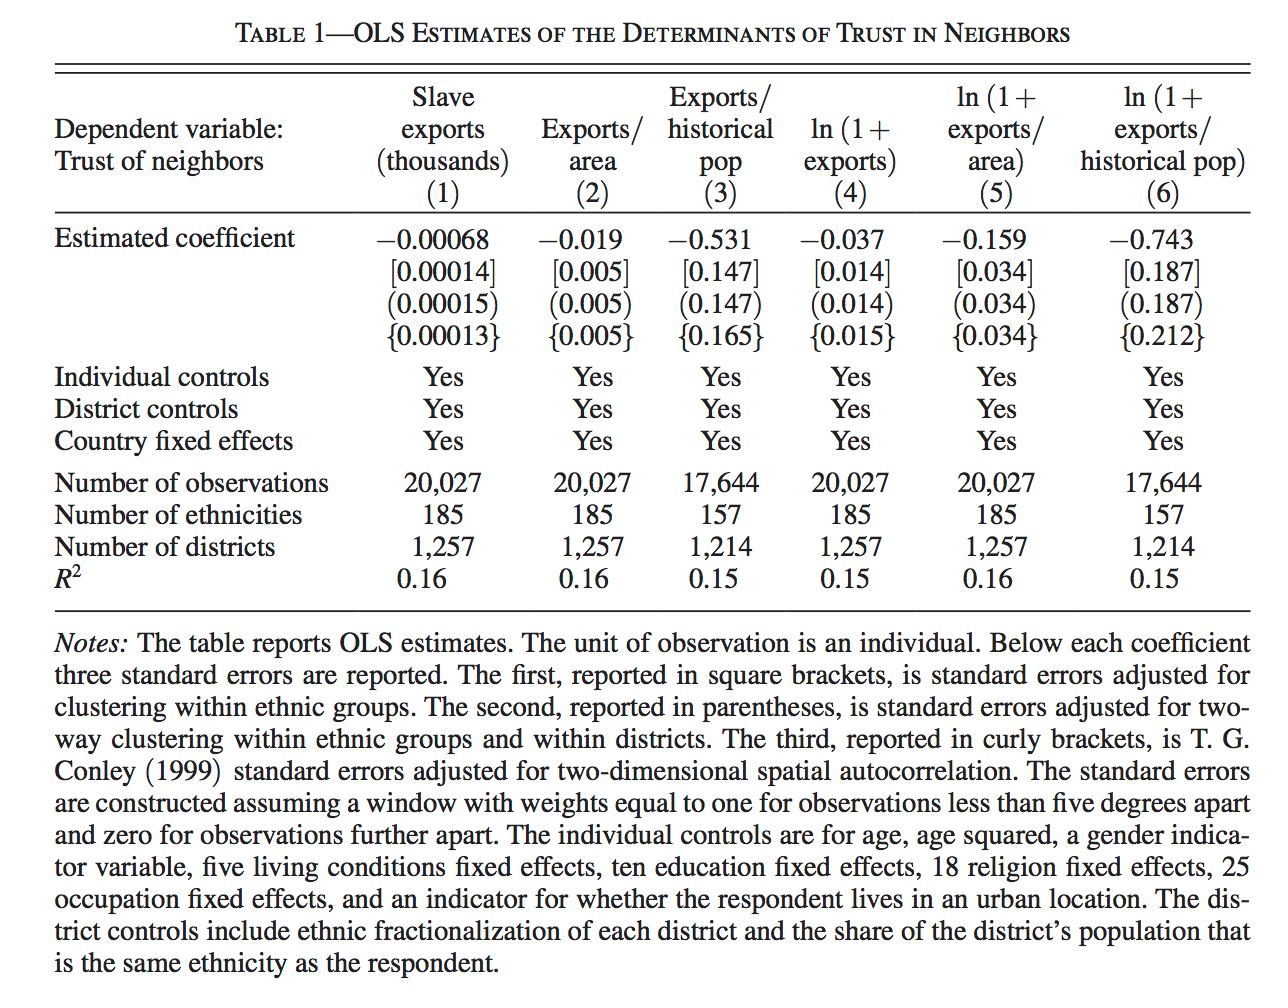
\includegraphics{./images/nunn_wantchekon_table1.png}

A very crude way to describe regression is through linear combinations.
The simplest linear combination is a one-to-one transformation.

Take the first number in Table 1, which is -0.00068. Now, multiply this
by \texttt{exports}

\begin{Shaded}
\begin{Highlighting}[]
\SpecialCharTok{{-}}\FloatTok{0.00068} \SpecialCharTok{*}\NormalTok{ X[, }\StringTok{"exports"}\NormalTok{]}
\end{Highlighting}
\end{Shaded}

\begin{verbatim}
 [1] -0.0002640778 -0.0004291640 -0.0006760487 -0.1241606061  0.0000000000
 [6]  0.0000000000 -0.4528563428 -0.0002363964 -0.0002957912  0.0000000000
\end{verbatim}

Now, just one more step. Make a new matrix with just exports and the
value 1

\begin{Shaded}
\begin{Highlighting}[]
\NormalTok{X2 }\OtherTok{\textless{}{-}} \FunctionTok{cbind}\NormalTok{(}\DecValTok{1}\NormalTok{, X[, }\StringTok{"exports"}\NormalTok{])}
\end{Highlighting}
\end{Shaded}

name this new column ``intercept''

\begin{Shaded}
\begin{Highlighting}[]
\FunctionTok{colnames}\NormalTok{(X2)}
\end{Highlighting}
\end{Shaded}

\begin{verbatim}
NULL
\end{verbatim}

\begin{Shaded}
\begin{Highlighting}[]
\FunctionTok{colnames}\NormalTok{(X2) }\OtherTok{\textless{}{-}} \FunctionTok{c}\NormalTok{(}\StringTok{"intercept"}\NormalTok{, }\StringTok{"exports"}\NormalTok{)}
\end{Highlighting}
\end{Shaded}

What are the dimensions of the matrix \texttt{X2}?

\begin{Shaded}
\begin{Highlighting}[]
\FunctionTok{dim}\NormalTok{(X2)}
\end{Highlighting}
\end{Shaded}

\begin{verbatim}
[1] 10  2
\end{verbatim}

Now consider a new matrix, called \texttt{B}.

\begin{Shaded}
\begin{Highlighting}[]
\NormalTok{B }\OtherTok{\textless{}{-}} \FunctionTok{matrix}\NormalTok{(}\FunctionTok{c}\NormalTok{(}\FloatTok{1.62}\NormalTok{, }\SpecialCharTok{{-}}\FloatTok{0.00068}\NormalTok{))}
\end{Highlighting}
\end{Shaded}

What are the dimensions of \texttt{B}?

\begin{Shaded}
\begin{Highlighting}[]
\FunctionTok{dim}\NormalTok{(B)}
\end{Highlighting}
\end{Shaded}

\begin{verbatim}
[1] 2 1
\end{verbatim}

What is the product of \texttt{X2} and \texttt{B}? From the dimensions,
can you tell if it will be conformable?

\begin{Shaded}
\begin{Highlighting}[]
\NormalTok{X2 }\SpecialCharTok{\%*\%}\NormalTok{ B}
\end{Highlighting}
\end{Shaded}

\begin{verbatim}
          [,1]
 [1,] 1.619736
 [2,] 1.619571
 [3,] 1.619324
 [4,] 1.495839
 [5,] 1.620000
 [6,] 1.620000
 [7,] 1.167144
 [8,] 1.619764
 [9,] 1.619704
[10,] 1.620000
\end{verbatim}

What is this multiplication doing in terms of equations?

\hypertarget{matrix-basics}{%
\section{Matrix Basics}\label{matrix-basics}}

Let's take a look at Matrices in the context of R

\begin{Shaded}
\begin{Highlighting}[]
\NormalTok{cen10 }\OtherTok{\textless{}{-}} \FunctionTok{read\_csv}\NormalTok{(}\StringTok{"data/input/usc2010\_001percent.csv"}\NormalTok{)}
\FunctionTok{head}\NormalTok{(cen10)}
\end{Highlighting}
\end{Shaded}

\begin{verbatim}
# A tibble: 6 x 4
  state         sex      age race       
  <chr>         <chr>  <dbl> <chr>      
1 New York      Female     8 White      
2 Ohio          Male      24 White      
3 Nevada        Male      37 White      
4 Michigan      Female    12 White      
5 Maryland      Female    18 Black/Negro
6 New Hampshire Male      50 White      
\end{verbatim}

What is the dimension of this dataframe? What does the number of rows
represent? What does the number of columns represent?

\begin{Shaded}
\begin{Highlighting}[]
\FunctionTok{dim}\NormalTok{(cen10)}
\end{Highlighting}
\end{Shaded}

\begin{verbatim}
[1] 30871     4
\end{verbatim}

\begin{Shaded}
\begin{Highlighting}[]
\FunctionTok{nrow}\NormalTok{(cen10)}
\end{Highlighting}
\end{Shaded}

\begin{verbatim}
[1] 30871
\end{verbatim}

\begin{Shaded}
\begin{Highlighting}[]
\FunctionTok{ncol}\NormalTok{(cen10)}
\end{Highlighting}
\end{Shaded}

\begin{verbatim}
[1] 4
\end{verbatim}

What variables does this dataset hold? What kind of information does it
have?

\begin{Shaded}
\begin{Highlighting}[]
\FunctionTok{colnames}\NormalTok{(cen10)}
\end{Highlighting}
\end{Shaded}

\begin{verbatim}
[1] "state" "sex"   "age"   "race" 
\end{verbatim}

We can access column vectors, or vectors that contain values of
variables by using the \$ sign

\begin{Shaded}
\begin{Highlighting}[]
\FunctionTok{head}\NormalTok{(cen10}\SpecialCharTok{$}\NormalTok{state)}
\end{Highlighting}
\end{Shaded}

\begin{verbatim}
[1] "New York"      "Ohio"          "Nevada"        "Michigan"     
[5] "Maryland"      "New Hampshire"
\end{verbatim}

\begin{Shaded}
\begin{Highlighting}[]
\FunctionTok{head}\NormalTok{(cen10}\SpecialCharTok{$}\NormalTok{race)}
\end{Highlighting}
\end{Shaded}

\begin{verbatim}
[1] "White"       "White"       "White"       "White"       "Black/Negro"
[6] "White"      
\end{verbatim}

We can look at a unique set of variable values by calling the unique
function

\begin{Shaded}
\begin{Highlighting}[]
\FunctionTok{unique}\NormalTok{(cen10}\SpecialCharTok{$}\NormalTok{state)}
\end{Highlighting}
\end{Shaded}

\begin{verbatim}
 [1] "New York"             "Ohio"                 "Nevada"              
 [4] "Michigan"             "Maryland"             "New Hampshire"       
 [7] "Iowa"                 "Missouri"             "New Jersey"          
[10] "California"           "Texas"                "Pennsylvania"        
[13] "Washington"           "West Virginia"        "Idaho"               
[16] "North Carolina"       "Massachusetts"        "Connecticut"         
[19] "Arkansas"             "Indiana"              "Wisconsin"           
[22] "Maine"                "Tennessee"            "Minnesota"           
[25] "Florida"              "Oklahoma"             "Montana"             
[28] "Georgia"              "Arizona"              "Colorado"            
[31] "Virginia"             "Illinois"             "Oregon"              
[34] "Kentucky"             "South Carolina"       "Kansas"              
[37] "Louisiana"            "Alabama"              "District of Columbia"
[40] "Mississippi"          "Utah"                 "Delaware"            
[43] "Nebraska"             "Alaska"               "New Mexico"          
[46] "South Dakota"         "Hawaii"               "Vermont"             
[49] "Rhode Island"         "Wyoming"              "North Dakota"        
\end{verbatim}

How many different states are represented (this dataset includes DC as a
state)?

\begin{Shaded}
\begin{Highlighting}[]
\FunctionTok{length}\NormalTok{(}\FunctionTok{unique}\NormalTok{(cen10}\SpecialCharTok{$}\NormalTok{state))}
\end{Highlighting}
\end{Shaded}

\begin{verbatim}
[1] 51
\end{verbatim}

Matrices are rectangular structures of numbers (they have to be numbers,
and they can't be characters).

A cross-tab can be considered a matrix:

\begin{Shaded}
\begin{Highlighting}[]
\FunctionTok{table}\NormalTok{(cen10}\SpecialCharTok{$}\NormalTok{race, cen10}\SpecialCharTok{$}\NormalTok{sex)}
\end{Highlighting}
\end{Shaded}

\begin{verbatim}
                                  
                                   Female  Male
  American Indian or Alaska Native    142   153
  Black/Negro                        2070  1943
  Chinese                             192   162
  Japanese                             51    26
  Other Asian or Pacific Islander     587   542
  Other race, nec                     877   962
  Three or more major races            37    51
  Two major races                     443   426
  White                             11252 10955
\end{verbatim}

\begin{Shaded}
\begin{Highlighting}[]
\NormalTok{cross\_tab }\OtherTok{\textless{}{-}} \FunctionTok{table}\NormalTok{(cen10}\SpecialCharTok{$}\NormalTok{race, cen10}\SpecialCharTok{$}\NormalTok{sex)}
\FunctionTok{dim}\NormalTok{(cross\_tab)}
\end{Highlighting}
\end{Shaded}

\begin{verbatim}
[1] 9 2
\end{verbatim}

\begin{Shaded}
\begin{Highlighting}[]
\NormalTok{cross\_tab[}\DecValTok{6}\NormalTok{, }\DecValTok{2}\NormalTok{]}
\end{Highlighting}
\end{Shaded}

\begin{verbatim}
[1] 962
\end{verbatim}

But a subset of your data -- individual values-- can be considered a
matrix too.

\begin{Shaded}
\begin{Highlighting}[]
\CommentTok{\# First 20 rows of the entire data}
\CommentTok{\# Below two lines of code do the same thing}
\NormalTok{cen10[}\DecValTok{1}\SpecialCharTok{:}\DecValTok{20}\NormalTok{, ]}
\end{Highlighting}
\end{Shaded}

\begin{verbatim}
# A tibble: 20 x 4
   state         sex      age race           
   <chr>         <chr>  <dbl> <chr>          
 1 New York      Female     8 White          
 2 Ohio          Male      24 White          
 3 Nevada        Male      37 White          
 4 Michigan      Female    12 White          
 5 Maryland      Female    18 Black/Negro    
 6 New Hampshire Male      50 White          
 7 Iowa          Female    51 White          
 8 Missouri      Female    41 White          
 9 New Jersey    Male      62 White          
10 California    Male      25 White          
11 Texas         Female    23 White          
12 Pennsylvania  Female    66 White          
13 California    Female    57 White          
14 Texas         Female    73 Other race, nec
15 California    Male      43 White          
16 Washington    Male      29 White          
17 Texas         Male       8 White          
18 Missouri      Male      78 White          
19 West Virginia Male      10 White          
20 Idaho         Female     9 White          
\end{verbatim}

\begin{Shaded}
\begin{Highlighting}[]
\NormalTok{cen10 }\SpecialCharTok{\%\textgreater{}\%} \FunctionTok{slice}\NormalTok{(}\DecValTok{1}\SpecialCharTok{:}\DecValTok{20}\NormalTok{)}
\end{Highlighting}
\end{Shaded}

\begin{verbatim}
# A tibble: 20 x 4
   state         sex      age race           
   <chr>         <chr>  <dbl> <chr>          
 1 New York      Female     8 White          
 2 Ohio          Male      24 White          
 3 Nevada        Male      37 White          
 4 Michigan      Female    12 White          
 5 Maryland      Female    18 Black/Negro    
 6 New Hampshire Male      50 White          
 7 Iowa          Female    51 White          
 8 Missouri      Female    41 White          
 9 New Jersey    Male      62 White          
10 California    Male      25 White          
11 Texas         Female    23 White          
12 Pennsylvania  Female    66 White          
13 California    Female    57 White          
14 Texas         Female    73 Other race, nec
15 California    Male      43 White          
16 Washington    Male      29 White          
17 Texas         Male       8 White          
18 Missouri      Male      78 White          
19 West Virginia Male      10 White          
20 Idaho         Female     9 White          
\end{verbatim}

\begin{Shaded}
\begin{Highlighting}[]
\CommentTok{\# Of the first 20 rows of the entire data, look at values of just race and age}
\CommentTok{\# Below two lines of code do the same thing}
\NormalTok{cen10[}\DecValTok{1}\SpecialCharTok{:}\DecValTok{20}\NormalTok{, }\FunctionTok{c}\NormalTok{(}\StringTok{"race"}\NormalTok{, }\StringTok{"age"}\NormalTok{)]}
\end{Highlighting}
\end{Shaded}

\begin{verbatim}
# A tibble: 20 x 2
   race              age
   <chr>           <dbl>
 1 White               8
 2 White              24
 3 White              37
 4 White              12
 5 Black/Negro        18
 6 White              50
 7 White              51
 8 White              41
 9 White              62
10 White              25
11 White              23
12 White              66
13 White              57
14 Other race, nec    73
15 White              43
16 White              29
17 White               8
18 White              78
19 White              10
20 White               9
\end{verbatim}

\begin{Shaded}
\begin{Highlighting}[]
\NormalTok{cen10 }\SpecialCharTok{\%\textgreater{}\%} \FunctionTok{slice}\NormalTok{(}\DecValTok{1}\SpecialCharTok{:}\DecValTok{20}\NormalTok{) }\SpecialCharTok{\%\textgreater{}\%} \FunctionTok{select}\NormalTok{(race, age)}
\end{Highlighting}
\end{Shaded}

\begin{verbatim}
# A tibble: 20 x 2
   race              age
   <chr>           <dbl>
 1 White               8
 2 White              24
 3 White              37
 4 White              12
 5 Black/Negro        18
 6 White              50
 7 White              51
 8 White              41
 9 White              62
10 White              25
11 White              23
12 White              66
13 White              57
14 Other race, nec    73
15 White              43
16 White              29
17 White               8
18 White              78
19 White              10
20 White               9
\end{verbatim}

A vector is a special type of matrix with only one column or only one
row

\begin{Shaded}
\begin{Highlighting}[]
\CommentTok{\# One column}
\NormalTok{cen10[}\DecValTok{1}\SpecialCharTok{:}\DecValTok{10}\NormalTok{, }\FunctionTok{c}\NormalTok{(}\StringTok{"age"}\NormalTok{)]}
\end{Highlighting}
\end{Shaded}

\begin{verbatim}
# A tibble: 10 x 1
     age
   <dbl>
 1     8
 2    24
 3    37
 4    12
 5    18
 6    50
 7    51
 8    41
 9    62
10    25
\end{verbatim}

\begin{Shaded}
\begin{Highlighting}[]
\NormalTok{cen10 }\SpecialCharTok{\%\textgreater{}\%} \FunctionTok{slice}\NormalTok{(}\DecValTok{1}\SpecialCharTok{:}\DecValTok{10}\NormalTok{) }\SpecialCharTok{\%\textgreater{}\%} \FunctionTok{select}\NormalTok{(}\FunctionTok{c}\NormalTok{(}\StringTok{"age"}\NormalTok{))}
\end{Highlighting}
\end{Shaded}

\begin{verbatim}
# A tibble: 10 x 1
     age
   <dbl>
 1     8
 2    24
 3    37
 4    12
 5    18
 6    50
 7    51
 8    41
 9    62
10    25
\end{verbatim}

\begin{Shaded}
\begin{Highlighting}[]
\CommentTok{\# One row}
\NormalTok{cen10[}\DecValTok{2}\NormalTok{, ]}
\end{Highlighting}
\end{Shaded}

\begin{verbatim}
# A tibble: 1 x 4
  state sex     age race 
  <chr> <chr> <dbl> <chr>
1 Ohio  Male     24 White
\end{verbatim}

\begin{Shaded}
\begin{Highlighting}[]
\NormalTok{cen10 }\SpecialCharTok{\%\textgreater{}\%} \FunctionTok{slice}\NormalTok{(}\DecValTok{2}\NormalTok{)}
\end{Highlighting}
\end{Shaded}

\begin{verbatim}
# A tibble: 1 x 4
  state sex     age race 
  <chr> <chr> <dbl> <chr>
1 Ohio  Male     24 White
\end{verbatim}

What if we want a special subset of the data? For example, what if I
only want the records of individuals in California? What if I just want
the age and race of individuals in California?

\begin{Shaded}
\begin{Highlighting}[]
\CommentTok{\# subset for CA rows}
\NormalTok{ca\_subset }\OtherTok{\textless{}{-}}\NormalTok{ cen10[cen10}\SpecialCharTok{$}\NormalTok{state }\SpecialCharTok{==} \StringTok{"California"}\NormalTok{, ]}

\NormalTok{ca\_subset\_tidy }\OtherTok{\textless{}{-}}\NormalTok{ cen10 }\SpecialCharTok{\%\textgreater{}\%} \FunctionTok{filter}\NormalTok{(state }\SpecialCharTok{==} \StringTok{"California"}\NormalTok{)}

\FunctionTok{all\_equal}\NormalTok{(ca\_subset, ca\_subset\_tidy)}
\end{Highlighting}
\end{Shaded}

\begin{verbatim}
[1] TRUE
\end{verbatim}

\begin{Shaded}
\begin{Highlighting}[]
\CommentTok{\# subset for CA rows and select age and race}
\NormalTok{ca\_subset\_age\_race }\OtherTok{\textless{}{-}}\NormalTok{ cen10[cen10}\SpecialCharTok{$}\NormalTok{state }\SpecialCharTok{==} \StringTok{"California"}\NormalTok{, }\FunctionTok{c}\NormalTok{(}\StringTok{"age"}\NormalTok{, }\StringTok{"race"}\NormalTok{)]}

\NormalTok{ca\_subset\_age\_race\_tidy }\OtherTok{\textless{}{-}}\NormalTok{ cen10 }\SpecialCharTok{\%\textgreater{}\%} \FunctionTok{filter}\NormalTok{(state }\SpecialCharTok{==} \StringTok{"California"}\NormalTok{) }\SpecialCharTok{\%\textgreater{}\%} \FunctionTok{select}\NormalTok{(age, race)}

\FunctionTok{all\_equal}\NormalTok{(ca\_subset\_age\_race, ca\_subset\_age\_race\_tidy)}
\end{Highlighting}
\end{Shaded}

\begin{verbatim}
[1] TRUE
\end{verbatim}

Some common operators that can be used to filter or to use as a
condition. Remember, you can use the unique function to look at the set
of all values a variable holds in the dataset.

\begin{Shaded}
\begin{Highlighting}[]
\CommentTok{\# all individuals older than 30 and younger than 70}
\NormalTok{s1 }\OtherTok{\textless{}{-}}\NormalTok{ cen10[cen10}\SpecialCharTok{$}\NormalTok{age }\SpecialCharTok{\textgreater{}} \DecValTok{30} \SpecialCharTok{\&}\NormalTok{ cen10}\SpecialCharTok{$}\NormalTok{age }\SpecialCharTok{\textless{}} \DecValTok{70}\NormalTok{, ]}
\NormalTok{s2 }\OtherTok{\textless{}{-}}\NormalTok{ cen10 }\SpecialCharTok{\%\textgreater{}\%} \FunctionTok{filter}\NormalTok{(age }\SpecialCharTok{\textgreater{}} \DecValTok{30} \SpecialCharTok{\&}\NormalTok{ age }\SpecialCharTok{\textless{}} \DecValTok{70}\NormalTok{)}
\FunctionTok{all\_equal}\NormalTok{(s1, s2)}
\end{Highlighting}
\end{Shaded}

\begin{verbatim}
[1] TRUE
\end{verbatim}

\begin{Shaded}
\begin{Highlighting}[]
\CommentTok{\# all individuals in either New York or California}
\NormalTok{s3 }\OtherTok{\textless{}{-}}\NormalTok{ cen10[cen10}\SpecialCharTok{$}\NormalTok{state }\SpecialCharTok{==} \StringTok{"New York"} \SpecialCharTok{|}\NormalTok{ cen10}\SpecialCharTok{$}\NormalTok{state }\SpecialCharTok{==} \StringTok{"California"}\NormalTok{, ]}
\NormalTok{s4 }\OtherTok{\textless{}{-}}\NormalTok{ cen10 }\SpecialCharTok{\%\textgreater{}\%} \FunctionTok{filter}\NormalTok{(state }\SpecialCharTok{==} \StringTok{"New York"} \SpecialCharTok{|}\NormalTok{ state }\SpecialCharTok{==} \StringTok{"California"}\NormalTok{)}
\FunctionTok{all\_equal}\NormalTok{(s3, s4)}
\end{Highlighting}
\end{Shaded}

\begin{verbatim}
[1] TRUE
\end{verbatim}

\begin{Shaded}
\begin{Highlighting}[]
\CommentTok{\# all individuals in any of the following states: California, Ohio, Nevada, Michigan}
\NormalTok{s5 }\OtherTok{\textless{}{-}}\NormalTok{ cen10[cen10}\SpecialCharTok{$}\NormalTok{state }\SpecialCharTok{\%in\%} \FunctionTok{c}\NormalTok{(}\StringTok{"California"}\NormalTok{, }\StringTok{"Ohio"}\NormalTok{, }\StringTok{"Nevada"}\NormalTok{, }\StringTok{"Michigan"}\NormalTok{), ]}
\NormalTok{s6 }\OtherTok{\textless{}{-}}\NormalTok{ cen10 }\SpecialCharTok{\%\textgreater{}\%} \FunctionTok{filter}\NormalTok{(state }\SpecialCharTok{\%in\%} \FunctionTok{c}\NormalTok{(}\StringTok{"California"}\NormalTok{, }\StringTok{"Ohio"}\NormalTok{, }\StringTok{"Nevada"}\NormalTok{, }\StringTok{"Michigan"}\NormalTok{))}
\FunctionTok{all\_equal}\NormalTok{(s5, s6)}
\end{Highlighting}
\end{Shaded}

\begin{verbatim}
[1] TRUE
\end{verbatim}

\begin{Shaded}
\begin{Highlighting}[]
\CommentTok{\# all individuals NOT in any of the following states: California, Ohio, Nevada, Michigan}
\NormalTok{s7 }\OtherTok{\textless{}{-}}\NormalTok{ cen10[}\SpecialCharTok{!}\NormalTok{(cen10}\SpecialCharTok{$}\NormalTok{state }\SpecialCharTok{\%in\%} \FunctionTok{c}\NormalTok{(}\StringTok{"California"}\NormalTok{, }\StringTok{"Ohio"}\NormalTok{, }\StringTok{"Nevada"}\NormalTok{, }\StringTok{"Michigan"}\NormalTok{)), ]}
\NormalTok{s8 }\OtherTok{\textless{}{-}}\NormalTok{ cen10 }\SpecialCharTok{\%\textgreater{}\%} \FunctionTok{filter}\NormalTok{(}\SpecialCharTok{!}\NormalTok{state }\SpecialCharTok{\%in\%} \FunctionTok{c}\NormalTok{(}\StringTok{"California"}\NormalTok{, }\StringTok{"Ohio"}\NormalTok{, }\StringTok{"Nevada"}\NormalTok{, }\StringTok{"Michigan"}\NormalTok{))}
\FunctionTok{all\_equal}\NormalTok{(s7, s8)}
\end{Highlighting}
\end{Shaded}

\begin{verbatim}
[1] TRUE
\end{verbatim}

\part{III Calculus}

\hypertarget{limits-precalc}{%
\chapter{Limits}\label{limits-precalc}}

Solving limits, i.e.~finding out the value of functions as its input
moves closer to some value, is important for the social scientist's
mathematical toolkit for two related tasks. The first is for the study
of calculus, which will be in turn useful to show where certain
functions are maximized or minimized. The second is for the study of
statistical inference, which is the study of inferring things about
things you cannot see by using things you can see.

\hypertarget{example-the-central-limit-theorem}{%
\section*{Example: The Central Limit
Theorem}\label{example-the-central-limit-theorem}}
\addcontentsline{toc}{section}{Example: The Central Limit Theorem}

Perhaps the most important theorem in statistics is the Central Limit
Theorem,

\leavevmode\vadjust pre{\hypertarget{thm-clt-lim}{}}%
\begin{theorem}[Central Limit Theorem (i.i.d. case)]\label{thm-clt-lim}

For any series of independent and identically distributed random
variables \(X_1, X_2, \cdots\), we know the distribution of its sum even
if we do not know the distribution of \(X\). The distribution of the sum
is a Normal distribution.

\[\frac{\bar{X}_n - \mu}{\sigma / \sqrt{n}} \xrightarrow{d} \text{Normal}(0, 1),\]

where \(\mu\) is the mean of \(X\) and \(\sigma\) is the standard
deviation of \(X\). The arrow is read as ``converges in distribution
to''. \(\text{Normal}(0, 1)\) indicates a Normal Distribution with mean
0 and variance 1.

That is, the limit of the distribution of the lefthand side is the
distribution of the righthand side.

\end{theorem}

The sign of a limit is the arrow ``\(\rightarrow\)''. Although we have
not yet covered probability so we have not described what distributions
and random variables are, it is worth foreshadowing the Central Limit
Theorem. The Central Limit Theorem is powerful because it gives us a
\emph{guarantee} of what would happen if \(n \rightarrow \infty\), which
in this case means we collected more data.

\hypertarget{example-the-law-of-large-numbers}{%
\section*{Example: The Law of Large
Numbers}\label{example-the-law-of-large-numbers}}
\addcontentsline{toc}{section}{Example: The Law of Large Numbers}

A finding that perhaps rivals the Central Limit Theorem is the Law of
Large Numbers:

\leavevmode\vadjust pre{\hypertarget{thm-lln-lim}{}}%
\begin{theorem}[(Weak) Law of Large Numbers]\label{thm-lln-lim}

For any draw of identically distributed independent variables with mean
\(\mu\), the sample average after \(n\) draws, \(\bar{X}_n\), converges
in probability to the true mean as \(n \rightarrow \infty\):

\[\lim\limits_{n\to \infty} P(|\bar{X}_n - \mu | > \varepsilon) = 0\]

A shorthand of which is \(\bar{X}_n \xrightarrow{p} \mu\), where the
arrow is read as ``converges in probability to''.

\end{theorem}

Intuitively, the more data, the more accurate is your guess. For
example, Figure~\ref{fig-llnsim} shows how the sample average from many
coin tosses converges to the true value : 0.5.

\begin{figure}

{\centering 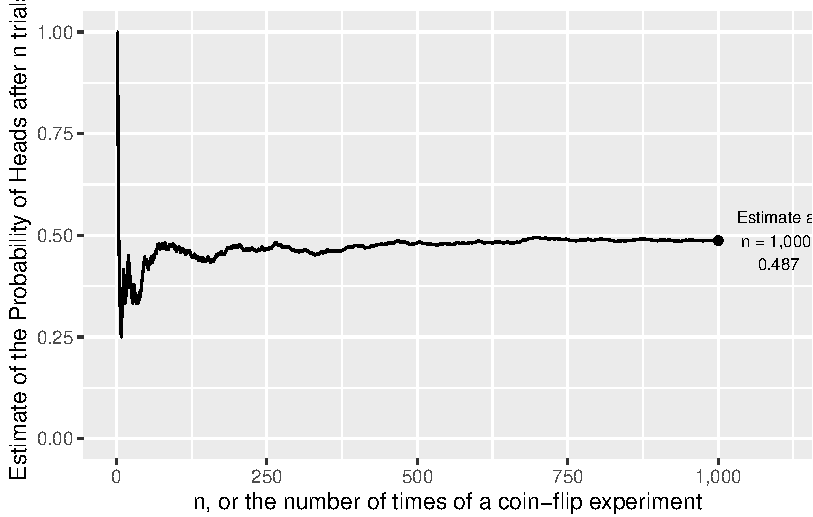
\includegraphics{./31_limits_files/figure-pdf/fig-llnsim-1.pdf}

}

\caption{\label{fig-llnsim}As the number of coin tosses goes to
infinity, the average probabiity of heads converges to 0.5}

\end{figure}

\hypertarget{sequences}{%
\section{Sequences}\label{sequences}}

We need a couple of steps until we get to limit theorems in probability.
First we will introduce a ``sequence'', then we will think about the
limit of a sequence, then we will think about the limit of a
\emph{function}.

A \textbf{sequence} \[\{x_n\}=\{x_1, x_2, x_3, \ldots, x_n\}\] is an
ordered set of real numbers, where \(x_1\) is the first term in the
sequence and \(y_n\) is the \(n\)th term. Generally, a sequence is
infinite, that is it extends to \(n=\infty\). We can also write the
sequence as \[\{x_n\}^\infty_{n=1}\]

where the subscript and superscript are read together as ``from 1 to
infinity.''

\leavevmode\vadjust pre{\hypertarget{exm-seqbehav}{}}%
\begin{example}[]\label{exm-seqbehav}

How do these sequences behave?

\begin{enumerate}
\def\labelenumi{\arabic{enumi}.}
\tightlist
\item
  \(\{A_n\}=\left\{ 2-\frac{1}{n^2} \right\}\)
\item
  \(\{B_n\}=\left\{\frac{n^2+1}{n} \right\}\)
\item
  \(\{C_n\}=\left\{(-1)^n \left(1-\frac{1}{n}\right) \right\}\)
\end{enumerate}

\end{example}

We find the sequence by simply ``plugging in'' the integers into each
\(n\). The important thing is to get a sense of how these numbers are
going to change. Example 1's numbers seem to come closer and closer to
2, but will it ever surpass 2? Example 2's numbers are also increasing
each time, but will it hit a limit? What is the pattern in Example 3?
Graphing helps you make this point more clearly. See the sequence of
\(n = 1, ...20\) for each of the three examples in
Figure~\ref{fig-seqabc}.

\begin{figure}

{\centering 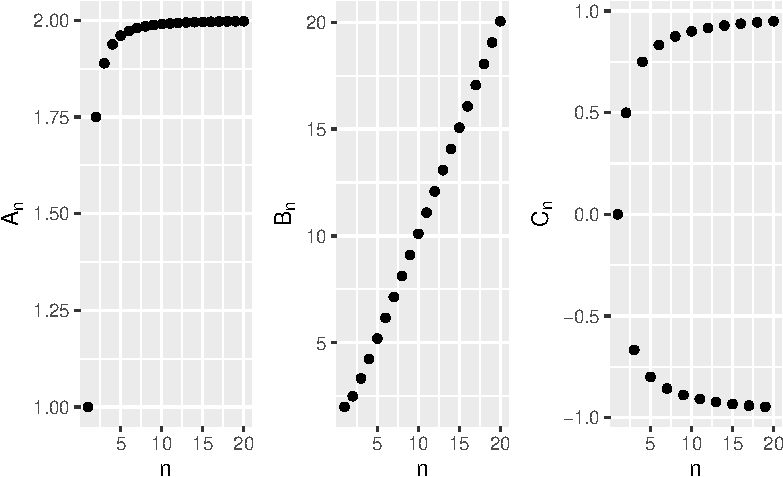
\includegraphics{./31_limits_files/figure-pdf/fig-seqabc-1.pdf}

}

\caption{\label{fig-seqabc}Behavior of Some Sequences}

\end{figure}

\hypertarget{the-limit-of-a-sequence}{%
\section{The Limit of a Sequence}\label{the-limit-of-a-sequence}}

The notion of ``converging to a limit'' is the behavior of the points in
Example~\ref{exm-seqbehav}. In some sense, that's the counterfactual we
want to know. What happens as \(n\rightarrow \infty\)?

\begin{enumerate}
\def\labelenumi{\arabic{enumi}.}
\tightlist
\item
  Sequences like 1 above that converge to a limit.
\item
  Sequences like 2 above that increase without bound.
\item
  Sequences like 3 above that neither converge nor increase without
  bound --- alternating over the number line.
\end{enumerate}

\leavevmode\vadjust pre{\hypertarget{def-seqlim}{}}%
\begin{definition}[Limit of a Sequence]\label{def-seqlim}

The sequence \(\{y_n\}\) has the limit \(L\), which we write as
\[\lim\limits_{n \to \infty} y_n =L,\] if for any \(\epsilon>0\) there
is an integer \(N\) (which depends on \(\epsilon\)) with the property
that \(|y_n -L|<\epsilon\) for each \(n>N\). \(\{y_n\}\) is said to
converge to \(L\). If the above does not hold, then \(\{y_n\}\)
diverges.

\end{definition}

We can also express the behavior of a sequence as bounded or not:

\begin{enumerate}
\def\labelenumi{\arabic{enumi}.}
\tightlist
\item
  Bounded: if \(|y_n|\le K\) for all \(n\)
\item
  Monotonically Increasing: \(y_{n+1}>y_n\) for all \(n\)
\item
  Monotonically Decreasing: \(y_{n+1}<y_n\) for all \(n\)
\end{enumerate}

A limit is \emph{unique}: If \(\{y_n\}\) converges, then the limit \(L\)
is unique.

If a sequence converges, then the sum of such sequences also converges.
Let \(\lim\limits_{n \to \infty} y_n = y\) and
\(\lim\limits_{n \to \infty} z_n =z\). Then

\begin{enumerate}
\def\labelenumi{\arabic{enumi}.}
\tightlist
\item
  \(\lim\limits_{n \to \infty} [k y_n + \ell z_n]= k y + \ell z\)
\item
  \(\lim\limits_{n \to \infty} y_n z_n = yz\)
\item
  \(\lim\limits_{n \to \infty} \frac{y_n}{z_n} = \frac{y}{z}\), provided
  \(z\neq 0\)
\end{enumerate}

This looks reasonable enough. The harder question, obviously is when the
parts of the fraction \emph{don't} converge. If
\(\lim_{n\to\infty} y_n = \infty\) and
\(\lim_{n\to\infty} z_n = \infty\), What is
\(\lim_{n\to\infty} y_n - z_n\)? What is
\(\lim_{n\to\infty} \frac{y_n}{z_n}\)?

It is nice for a sequence to converge in limit. We want to know if
complex-looking sequences converge or not. The name of the game here is
to break that complex sequence up into sums of simple fractions where
\(n\) only appears in the denominator: \(\frac{1}{n}, \frac{1}{n^2}\),
and so on. Each of these will converge to 0, because the denominator
gets larger and larger. Then, because of the properties above, we can
then find the final sequence.

\leavevmode\vadjust pre{\hypertarget{exm-limseq}{}}%
\begin{example}[]\label{exm-limseq}

Find the limit of

\[\lim_{n\to \infty} \frac{n + 3}{n}.\]

At first glance, \(n + 3\) and \(n\) both grow to \(\infty\), so it
looks like we need to divide infinity by infinity. However, we can
express this fraction as a sum, then the limits apply separately:

\[\lim_{n\to \infty} \frac{n + 3}{n} = \lim_{n\to \infty} \left(1 + \frac{3}{n}\right) =  \underbrace{\lim_{n\to \infty}1}_{1} +  \underbrace{\lim_{n\to \infty}\left(\frac{3}{n}\right)}_{0}\]

so, the limit is actually 1.

\end{example}

After some practice, the key to intuition is whether one part of the
fraction grows ``faster'' than another. If the denominator grows faster
to infinity than the numerator, then the fraction will converge to 0,
even if the numerator will also increase to infinity. In a sense, limits
show how not all infinities are the same.

\leavevmode\vadjust pre{\hypertarget{exr-limseq2}{}}%
\begin{exercise}[]\label{exr-limseq2}

Find the following limits of sequences, then explain in English the
intuition for why that is the case.

\begin{enumerate}
\def\labelenumi{\arabic{enumi}.}
\tightlist
\item
  \(\lim\limits_{n\to\infty} \frac{2n}{n^2 + 1}\)
\item
  \(\lim\limits_{n\to\infty} (n^3 - 100n^2)\)
\end{enumerate}

\end{exercise}

\hypertarget{limitsfun}{%
\section{Limits of a Function}\label{limitsfun}}

We've now covered functions and just covered limits of sequences, so now
is the time to combine the two.

A function \(f\) is a compact representation of some behavior we care
about. Like for sequences, we often want to know if \(f(x)\) approaches
some number \(L\) as its independent variable \(x\) moves to some number
\(c\) (which is usually 0 or \(\pm\infty\)). If it does, we say that the
limit of \(f(x)\), as \(x\) approaches \(c\), is \(L\):
\(\lim\limits_{x \to c} f(x)=L\). Unlike a sequence, \(x\) is a
continuous number, and we can move in decreasing order as well as
increasing.

For a limit \(L\) to exist, the function \(f(x)\) must approach \(L\)
from both the left (increasing) and the right (decreasing).

\leavevmode\vadjust pre{\hypertarget{def-limfun}{}}%
\begin{definition}[Limit of a function]\label{def-limfun}

Let \(f(x)\) be defined at each point in some open interval containing
the point \(c\). Then \(L\) equals \(\lim\limits_{x \to c} f(x)\) if for
any (small positive) number \(\epsilon\), there exists a corresponding
number \(\delta>0\) such that if \(0<|x-c|<\delta\), then
\(|f(x)-L|<\epsilon\).

\end{definition}

A neat, if subtle result is that \(f(x)\) does not necessarily have to
be defined at \(c\) for \(\lim\limits_{x \to c}\) to exist.

\leavevmode\vadjust pre{\hypertarget{prp-limfun}{}}%
\begin{proposition}[]\label{prp-limfun}

Let \(f\) and \(g\) be functions with \(\lim\limits_{x \to c} f(x)=k\)
and \(\lim\limits_{x \to c} g(x)=\ell\).

\begin{enumerate}
\def\labelenumi{\arabic{enumi}.}
\tightlist
\item
  \(\lim\limits_{x \to c}[f(x)+g(x)]=\lim\limits_{x \to c} f(x)+ \lim\limits_{x \to c} g(x)\)
\item
  \(\lim\limits_{x \to c} kf(x) = k\lim\limits_{x \to c} f(x)\)
\item
  \(\lim\limits_{x \to c} f(x) g(x) = \left[\lim\limits_{x \to c} f(x)\right]\cdot \left[\lim\limits_{x \to c} g(x)\right]\)
\item
  \(\lim\limits_{x \to c} \frac{f(x)}{g(x)} = \frac{\lim\limits_{x \to c} f(x)}{\lim\limits_{x \to c} g(x)}\),
  provided \(\lim\limits_{x \to c} g(x)\ne 0\).
\end{enumerate}

\end{proposition}

Simple limits of functions can be solved as we did limits of sequences.
Just be careful which part of the function is changing.

\leavevmode\vadjust pre{\hypertarget{exm-limfun1}{}}%
\begin{example}[]\label{exm-limfun1}

Find the limit of the following functions.

\begin{enumerate}
\def\labelenumi{\arabic{enumi}.}
\tightlist
\item
  \(\lim_{x \to c} k\)
\item
  \(\lim_{x \to c} x\)
\item
  \(\lim_{x\to 2} (2x-3)\)
\item
  \(\lim_{x \to c} x^n\)
\end{enumerate}

\end{example}

Limits can get more complex in roughly two ways. First, the functions
may become large polynomials with many moving pieces. Second,the
functions may become discontinuous.

The function can be thought of as a more general or ``smooth'' version
of sequences. For example,

\leavevmode\vadjust pre{\hypertarget{exr-limfunmax}{}}%
\begin{exercise}[]\label{exr-limfunmax}

Find the limit of

\[\lim_{x\to\infty} \frac{(x^4 +3x−99)(2−x^5)}{(18x^7 +9x^6 −3x^2 −1)(x+1)}\]

\end{exercise}

Now, the functions will become a bit more complex:

\leavevmode\vadjust pre{\hypertarget{exr-discontlim}{}}%
\begin{exercise}[]\label{exr-discontlim}

Solve the following limits of functions

\begin{enumerate}
\def\labelenumi{\arabic{enumi}.}
\tightlist
\item
  \(\lim\limits_{x\to 0} |x|\)
\item
  \(\lim\limits_{x\to 0} \left(1+\frac{1}{x^2}\right)\)
\end{enumerate}

\end{exercise}

So there are a few more alternatives about what a limit of a function
could be:

\begin{enumerate}
\def\labelenumi{\arabic{enumi}.}
\tightlist
\item
  Right-hand limit: The value approached by \(f(x)\) when you move from
  right to left.
\item
  Left-hand limit: The value approached by \(f(x)\) when you move from
  left to right.
\item
  Infinity: The value approached by \(f(x)\) as x grows infinitely
  large. Sometimes this may be a number; sometimes it might be
  \(\infty\) or \(-\infty\).
\item
  Negative infinity: The value approached by \(f(x)\) as x grows
  infinitely negative. Sometimes this may be a number; sometimes it
  might be \(\infty\) or \(-\infty\).
\end{enumerate}

The distinction between left and right becomes important when the
function is not determined for some values of \(x\). What are those
cases in the examples below?

\begin{figure}

{\centering \includegraphics{./31_limits_files/figure-pdf/unnamed-chunk-2-1.pdf}

}

\caption{Functions which are not defined in some areas}

\end{figure}

\hypertarget{continuity}{%
\section{Continuity}\label{continuity}}

To repeat a finding from the limits of functions: \(f(x)\) does not
necessarily have to be defined at \(c\) for \(\lim\limits_{x \to c}\) to
exist. Functions that have breaks in their lines are called
discontinuous. Functions that have no breaks are called continuous.
Continuity is a concept that is more fundamental to, but related to that
of ``differentiability'', which we will cover next in calculus.

\leavevmode\vadjust pre{\hypertarget{def-conti}{}}%
\begin{definition}[Continuity'']\label{def-conti}

Suppose that the domain of the function \(f\) includes an open interval
containing the point \(c\). Then \(f\) is continuous at \(c\) if
\(\lim\limits_{x \to c} f(x)\) exists and if
\(\lim\limits_{x \to c} f(x)=f(c)\). Further, \(f\) is continuous on an
open interval \((a,b)\) if it is continuous at each point in the
interval.

\end{definition}

To prove that a function is continuous for all points is beyond this
practical introduction to math, but the general intuition can be grasped
by graphing.

\leavevmode\vadjust pre{\hypertarget{exm-contdiscont}{}}%
\begin{example}[]\label{exm-contdiscont}

For each function, determine if it is continuous or discontinuous.

\begin{enumerate}
\def\labelenumi{\arabic{enumi}.}
\tightlist
\item
  \(f(x) = \sqrt{x}\)
\item
  \(f(x) = e^x\)
\item
  \(f(x) = 1 + \frac{1}{x^2}\)
\item
  \(f(x) = \text{floor}(x)\).
\end{enumerate}

The floor is the smaller of the two integers bounding a number. So
\(\text{floor}(x = 2.999) = 2\), \(\text{floor}(x = 2.0001) = 2\), and
\(\text{floor}(x = 2) = 2.\)

\end{example}

\begin{solution}

In Figure Figure~\ref{fig-contdiscont}, we can see that the first two
functions are continuous, and the next two are discontinuous.
\(f(x) = 1 + \frac{1}{x^2}\) is discontinuous at \(x= 0\), and
\(f(x) = \text{floor}(x)\) is discontinuous at each whole number.

\end{solution}

\begin{figure}

{\centering 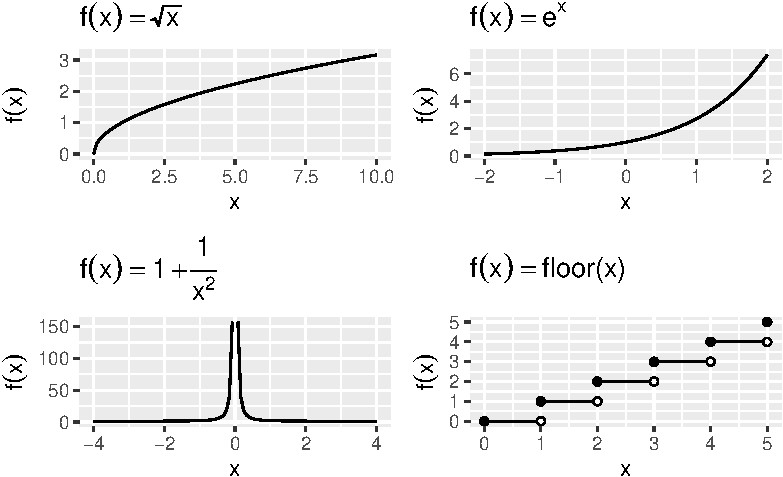
\includegraphics{./31_limits_files/figure-pdf/fig-contdiscont-1.pdf}

}

\caption{\label{fig-contdiscont}Continuous and Discontinuous Functions}

\end{figure}

Some properties of continuous functions:

\hypertarget{prop-conti}{}
\begin{enumerate}
\def\labelenumi{\arabic{enumi}.}
\tightlist
\item
  If \(f\) and \(g\) are continuous at point \(c\), then \(f+g\),
  \(f-g\), \(f \cdot g\), \(|f|\), and \(\alpha f\) are continuous at
  point \(c\) also. \(f/g\) is continuous, provided \(g(c)\ne 0\).
\item
  Boundedness: If \(f\) is continuous on the closed bounded interval
  \([a,b]\), then there is a number \(K\) such that \(|f(x)|\le K\) for
  each \(x\) in \([a,b]\).
\item
  Max/Min: If \(f\) is continuous on the closed bounded interval
  \([a,b]\), then \(f\) has a maximum and a minimum on \([a,b]\). They
  may be located at the end points.
\end{enumerate}

\leavevmode\vadjust pre{\hypertarget{exr-discontdraw}{}}%
\begin{exercise}[]\label{exr-discontdraw}

Let \[f(x) = \frac{x^2 + 2x}{x}.\]

\begin{enumerate}
\def\labelenumi{\arabic{enumi}.}
\tightlist
\item
  Graph the function. Is it defined everywhere?
\item
  What is the functions limit at \(x \rightarrow 0\)?
\end{enumerate}

\end{exercise}

\hypertarget{answers-to-examples}{%
\section*{Answers to Examples}\label{answers-to-examples}}
\addcontentsline{toc}{section}{Answers to Examples}

Example~\ref{exm-seqbehav}

\emph{Solution.}

\begin{enumerate}
\def\labelenumi{\arabic{enumi}.}
\tightlist
\item
  \(\{A_n\}=\left\{ 2-\frac{1}{n^2} \right\} = \left\{1, \frac{7}{4}, \frac{17}{9}, \frac{31}{16}, \frac{49}{25}, \ldots\right\} = 2\)
\item
  \(\{B_n\}=\left\{\frac{n^2+1}{n} \right\} = \left\{2, \frac{5}{2}, \frac{10}{3}, \frac{17}{4}..., \right\}\)
\item
  \(\{C_n\}=\left\{(-1)^n \left(1-\frac{1}{n}\right) \right\} = \left\{0, \frac{1}{2}, -\frac{2}{3}, \frac{3}{4}, -\frac{4}{5}\right\}\)
\end{enumerate}

Exercise~\ref{exr-limseq2}

\begin{solution}

Plot the function and you'll see the following limits:

\begin{enumerate}
\def\labelenumi{\arabic{enumi}.}
\tightlist
\item
  \(0\)
\item
  \(\infty\)
\end{enumerate}

\end{solution}

Example~\ref{exm-limfun1}

\emph{Solution.}

\begin{enumerate}
\def\labelenumi{\arabic{enumi}.}
\tightlist
\item
  \(k\)
\item
  \(c\)
\item
  \(\lim_{x\to 2} (2x-3) = 2\lim\limits_{x\to 2} x - 3\lim\limits_{x\to 2} 1 = 1\)
\item
  \(\lim_{x \to c} x^n = \lim\limits_{x \to c} x \cdots[\lim\limits_{x \to c} x] = c\cdots c =c^n\)
\end{enumerate}

Exercise~\ref{exr-limfunmax}

\begin{solution}

Although this function seems large, the thing our eyes should focus on
is where the highest order polynomial remains. That will grow the
fastest, so if the highest order term is on the denominator, the
fraction will converge to 0, if it is on the numerator it will converge
to negative infinity. Previewing the multiplication by hand, we can see
that the \(-x^9\) on the numerator will be the largest power. So the
answer will be \(-\infty\). We can also confirm this by writing out
fractions:

\[\begin{align*}  
& \lim_{x\to\infty}\frac{\left(1 + \frac{3}{x^3} - \frac{99}{4x^4}\right)\left(-\frac{2}{x^5} + 1\right)}{\left(1 + \frac{9}{18x} - \frac{3}{18x^5} - \frac{1}{18x^7} \right)\left(1 + \frac{1}{x}\right)} \\
&\times \frac{x^4}{1} \times -\frac{x^5}{1} \times \frac{1}{18x^7}\times \frac{1}{x}\\
=& 1 \times \lim_{-x\to\infty} \frac{x}{18}
\end{align*}\]

\end{solution}

Exercise~\ref{exr-discontdraw}

\begin{solution}

See Figure~\ref{fig-hole-0}. We can say \(\lim_{x\to 0}f(x) = 2\). Note
that we can express \[f(x) = 
    \left\{
    \begin{array}{ll}
        x+2 & x \neq 2; \\
        \textrm{undefined} & x = 2 \\
    \end{array} 
    \right.\]

\end{solution}

\begin{figure}

{\centering 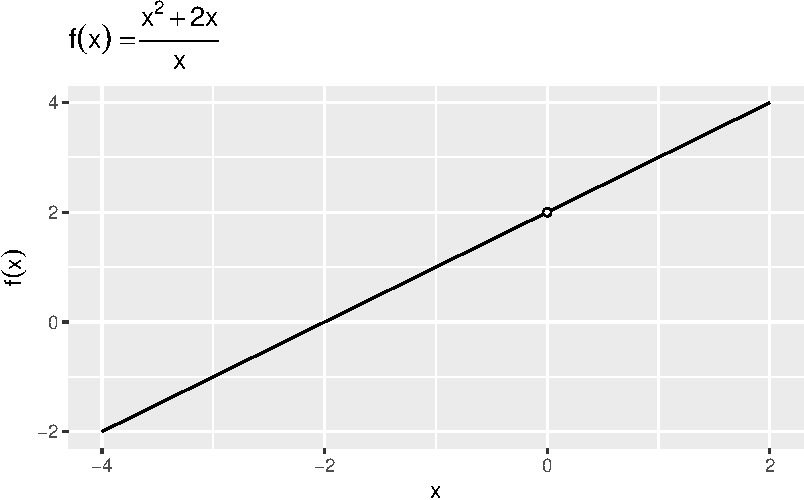
\includegraphics{./31_limits_files/figure-pdf/fig-hole-0-1.pdf}

}

\caption{\label{fig-hole-0}A function undedefined at x = 0}

\end{figure}

\hypertarget{derivatives}{%
\chapter{Differential Calculus}\label{derivatives}}

Calculus is a fundamental part of any type of statistics exercise.
Although you may not be taking derivatives and integral in your daily
work as an analyst, calculus undergirds many concepts we use:
maximization, expectation, and cumulative probability.

\hypertarget{sec-derivintro}{%
\section{Derivatives}\label{sec-derivintro}}

The derivative of \(f\) at \(x\) is its rate of change at \(x\): how
much \(f(x)\) changes with a change in \(x\). The rate of change is a
fraction --- rise over run --- but because not all lines are straight
and the rise over run formula will give us different values depending on
the range we examine, we need to take a limit.

\leavevmode\vadjust pre{\hypertarget{def-derivative}{}}%
\begin{definition}[Derivative]\label{def-derivative}

Let \(f\) be a function whose domain includes an open interval
containing the point \(x\). The derivative of \(f\) at \(x\) is given by

\[\frac{d}{dx}f(x) =\lim\limits_{h\to 0} \frac{f(x+h)-f(x)}{(x+h)-x} = \lim\limits_{h\to 0} \frac{f(x+h)-f(x)}{h}\]

There are a two main ways to denote a derivate:

\begin{itemize}
\tightlist
\item
  Leibniz Notation: \(\frac{d}{dx}(f(x))\)
\item
  Prime or Lagrange Notation: \(f'(x)\)
\end{itemize}

\end{definition}

If \(f(x)\) is a straight line, the derivative is the slope. For a
curve, the slope changes by the values of \(x\), so the derivative is
the slope of the line tangent to the curve at \(x\). See, For example,
Figure~\ref{fig-derivsimple}.

\begin{figure}

{\centering 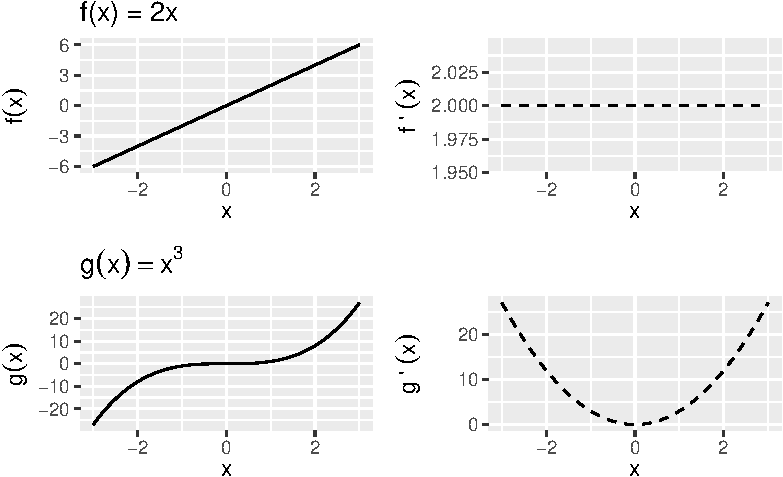
\includegraphics{./32_derivatives_files/figure-pdf/fig-derivsimple-1.pdf}

}

\caption{\label{fig-derivsimple}The Derivative as a Slope}

\end{figure}

If \(f'(x)\) exists at a point \(x_0\), then \(f\) is said to be
\textbf{differentiable} at \(x_0\). That also implies that \(f(x)\) is
continuous at \(x_0\).

\hypertarget{properties-of-derivatives}{%
\subsection*{Properties of
derivatives}\label{properties-of-derivatives}}
\addcontentsline{toc}{subsection}{Properties of derivatives}

Suppose that \(f\) and \(g\) are differentiable at \(x\) and that
\(\alpha\) is a constant. Then the functions \(f\pm g\), \(\alpha f\),
\(f g\), and \(f/g\) (provided \(g(x)\ne 0\)) are also differentiable at
\(x\). Additionally,

\textbf{Constant rule:} \[\left[k f(x)\right]' = k f'(x)\]

\textbf{Sum rule:} \[\left[f(x)\pm g(x)\right]' = f'(x)\pm g'(x)\]

With a bit more algebra, we can apply the definition of derivatives to
get a formula for of the derivative of a product and a derivative of a
quotient.

\textbf{Product rule:}
\[\left[f(x)g(x)\right]^\prime = f^\prime(x)g(x)+f(x)g^\prime(x)\]

\textbf{Quotient rule:}
\[\left[f(x)/g(x)\right]^\prime = \frac{f^\prime(x)g(x) - f(x)g^\prime(x)}{[g(x)]^2}, ~g(x)\neq 0\]

Finally, one way to think of the power of derivatives is that it takes a
function a notch down in complexity. The power rule applies to any
higher-order function:

\textbf{Power rule:} \[\left[x^k\right]^\prime = k x^{k-1}\]

For any real number \(k\) (that is, both whole numbers and fractions).
The power rule is proved \textbf{by induction}, a neat method of proof
used in many fundamental applications to prove that a general statement
holds for every possible case, even if there are countably infinite
cases. We'll show a simple case where \(k\) is an integer here.

\begin{proof}

We would like to prove that

\[\left[x^k\right]^\prime = k x^{k-1}\]

for any integer \(k\).

First, consider the first case (the base case) of \(k = 1\). We can show
by the definition of derivatives (setting \(f(x) = x^1 = 1\)) that

\[[x^1]^\prime = \lim_{h \rightarrow 0}\frac{(x + h) - x}{(x + h) - x}= 1.\]

Because \(1\) is also expressed as \(1 x^{1- 1}\), the statement we want
to prove holds for the case \(k =1\).

Now, \emph{assume} that the statement holds for some integer \(m\). That
is, assume

\[\left[x^m\right]^\prime = m x^{m-1}\]

Then, for the case \(m + 1\), using the product rule above, we can
simplify

\[\begin{align*}
  \left[x^{m + 1}\right]^\prime &= [x^{m}\cdot x]^\prime\\
  &= (x^m)^\prime\cdot x + (x^m)\cdot (x)^\prime\\
  &= m x^{m - 1}\cdot x + x^m ~~\because \text{by previous assumption}\\
  &= mx^m + x^m\\
  &= (m + 1)x^m\\
  &= (m + 1)x^{(m + 1) - 1}
  \end{align*}\]

Therefore, the rule holds for the case \(k = m + 1\) once we have
assumed it holds for \(k = m\). Combined with the first case, this
completes proof by induction -- we have now proved that the statement
holds for all integers \(k = 1, 2, 3, \cdots\).

To show that it holds for real fractions as well, we can prove
expressing that exponent by a fraction of two integers.

\end{proof}

These ``rules'' become apparent by applying the definition of the
derivative above to each of the things to be ``derived'', but these come
up so frequently that it is best to repeat until it is muscle memory.

\leavevmode\vadjust pre{\hypertarget{exr-introderivatives}{}}%
\begin{exercise}[]\label{exr-introderivatives}

For each of the following functions, find the first-order derivative
\(f^\prime(x)\).

\begin{enumerate}
\def\labelenumi{\arabic{enumi}.}
\tightlist
\item
  \(f(x)=c\)
\item
  \(f(x)=x\)
\item
  \(f(x)=x^2\)
\item
  \(f(x)=x^3\)
\item
  \(f(x)=\frac{1}{x^2}\)
\item
  \(f(x)=(x^3)(2x^4)\)
\item
  \(f(x) = x^4 - x^3 + x^2 - x + 1\)
\item
  \(f(x) = (x^2 + 1)(x^3 - 1)\)
\item
  \(f(x) = 3x^2 + 2x^{1/3}\)
\item
  \(f(x)=\frac{x^2+1}{x^2-1}\)
\end{enumerate}

\end{exercise}

\hypertarget{derivpoly}{%
\section{Higher-Order Derivatives}\label{derivpoly}}

The first derivative is applying the definition of derivatives on the
function, and it can be expressed as

\[f'(x),  ~~ y',  ~~ \frac{d}{dx}f(x), ~~ \frac{dy}{dx}\]

We can keep applying the differentiation process to functions that are
themselves derivatives. The derivative of \(f'(x)\) with respect to
\(x\), would then be
\[f''(x)=\lim\limits_{h\to 0}\frac{f'(x+h)-f'(x)}{h}\] and we can
therefore call it the \textbf{Second derivative:}

\[f''(x), ~~ y'', ~~ \frac{d^2}{dx^2}f(x), ~~ \frac{d^2y}{dx^2}\]

Similarly, the derivative of \(f''(x)\) would be called the third
derivative and is denoted \(f'''(x)\). And by extension, the \textbf{nth
derivative} is expressed as \(\frac{d^n}{dx^n}f(x)\),
\(\frac{d^ny}{dx^n}\).

\leavevmode\vadjust pre{\hypertarget{exm-succ-der}{}}%
\begin{example}[]\label{exm-succ-der}

\[\begin{align*}
f(x) &=x^3\\
f^{\prime}(x) &=3x^2\\
f^{\prime\prime}(x) &=6x \\
f^{\prime\prime\prime}(x) &=6\\
f^{\prime\prime\prime\prime}(x) &=0\\
\end{align*}\]

\end{example}

Earlier, in Section~\ref{sec-derivintro}, we said that if a function
differentiable at a given point, then it must be continuous. Further, if
\(f'(x)\) is itself continuous, then \(f(x)\) is called continuously
differentiable. All of this matters because many of our findings about
optimization rely on differentiation, and so we want our function to be
differentiable in as many layers. A function that is continuously
differentiable infinitly is called ``smooth''. Some examples:
\(f(x) = x^2\), \(f(x) = e^x\).

\hypertarget{the-chain-rule}{%
\section{The Chain Rule}\label{the-chain-rule}}

As useful as the above rules are, many functions you'll see won't fit
neatly in each case immediately. Instead, they will be functions of
functions. For example, the difference between \(x^2 + 1^2\) and
\((x^2 + 1)^2\) may look trivial, but the sum rule can be easily applied
to the former, while it's actually not obvious what do with the latter.

\textbf{Composite functions} are formed by substituting one function
into another and are denoted by \[(f\circ g)(x)=f[g(x)].\] To form
\(f[g(x)]\), the range of \(g\) must be contained (at least in part)
within the domain of \(f\). The domain of \(f\circ g\) consists of all
the points in the domain of \(g\) for which \(g(x)\) is in the domain of
\(f\).

\leavevmode\vadjust pre{\hypertarget{exm-}{}}%
\begin{example}[]\label{exm-}

Let \(f(x)=\ln x\) for \(0<x<\infty\) and \(g(x)=x^2\) for
\(-\infty<x<\infty\).

Then

\[(f\circ g)(x)=\ln x^2, -\infty<x<\infty - \{0\}\]

Also

\[(g\circ f)(x)=[\ln x]^2, 0<x<\infty\]

Notice that \(f\circ g\) and \(g\circ f\) are not the same functions.

\end{example}

With the notation of composite functions in place, now we can introduce
a helpful additional rule that will deal with a derivative of composite
functions as a chain of concentric derivatives.

\textbf{Chain Rule}:

Let \(y=(f\circ g)(x)= f[g(x)]\). The derivative of \(y\) with respect
to \(x\) is \[\frac{d}{dx} \{ f[g(x)] \} = f'[g(x)] g'(x)\]

We can read this as: ``the derivative of the composite function \(y\) is
the derivative of \(f\) evaluated at \(g(x)\), times the derivative of
\(g\).''

The chain rule can be thought of as the derivative of the ``outside''
times the derivative of the ``inside'', remembering that the derivative
of the outside function is evaluated at the value of the inside
function.

\begin{itemize}
\tightlist
\item
  The chain rule can also be written as
  \[\frac{dy}{dx}=\frac{dy}{dg(x)} \frac{dg(x)}{dx}\] This expression
  does not imply that the \(dg(x)\)'s cancel out, as in fractions. They
  are part of the derivative notation and you can't separate them out or
  cancel them.)
\end{itemize}

\leavevmode\vadjust pre{\hypertarget{exm-tothesix}{}}%
\begin{example}[]\label{exm-tothesix}

Find \(f^\prime(x)\) for \(f(x) = (3x^2+5x-7)^6\).

\end{example}

The direct use of a chain rule is when the exponent of is itself a
function, so the power rule could not have applied generaly:

\textbf{Generalized Power Rule}:

If \(f(x)=[g(x)]^p\) for any rational number \(p\),
\[f^\prime(x) =p[g(x)]^{p-1}g^\prime(x)\]

\hypertarget{derivatives-of-logs-and-exponents}{%
\section{Derivatives of logs and
exponents}\label{derivatives-of-logs-and-exponents}}

Natural logs and exponents (they are inverses of each other; see
Prerequisites) crop up everywhere in statistics. Their derivative is a
special case from the above, but quite elegant.

\leavevmode\vadjust pre{\hypertarget{thm-derivexplog}{}}%
\begin{theorem}[]\label{thm-derivexplog}

The functions \(e^x\) and the natural logarithm \(\ln(x)\) are
continuous and differentiable in their domains, and their first derivate
is

\[(e^x)^\prime = e^x\]

\[\ln(x)^\prime = \frac{1}{x}\]

Also, when these are composite functions, it follows by the generalized
power rule that

\[\left(e^{g(x)}\right)^\prime = e^{g(x)} \cdot g^\prime(x)\]

\[\left(\ln g(x)\right)^\prime = \frac{g^\prime(x)}{g(x)}, ~~\text{if}~~ g(x) > 0\]

\end{theorem}

We will relegate the proofs to small excerpts.

\hypertarget{derivatives-of-exponents}{%
\subsection*{Derivatives of exponents}\label{derivatives-of-exponents}}
\addcontentsline{toc}{subsection}{Derivatives of exponents}

To repeat the main rule in Theorem~\ref{thm-derivexplog}, the intuition
is that

\begin{enumerate}
\def\labelenumi{\arabic{enumi}.}
\tightlist
\item
  Derivative of \(e^x\) is itself: \(\frac{d}{dx}e^x = e^x\) (See
  Figure~\ref{fig-derivexponent})
\item
  Same thing if there were a constant in front:
  \(\frac{d}{dx}\alpha e^x = \alpha e^x\)
\item
  Same thing no matter how many derivatives there are in front:
  \(\frac{d^n}{dx^n} \alpha e^x = \alpha e^x\)
\item
  Chain Rule: When the exponent is a function of \(x\), remember to take
  derivative of that function and add to product.
  \(\frac{d}{dx}e^{g(x)}= e^{g(x)} g^\prime(x)\)
\end{enumerate}

\begin{figure}

{\centering 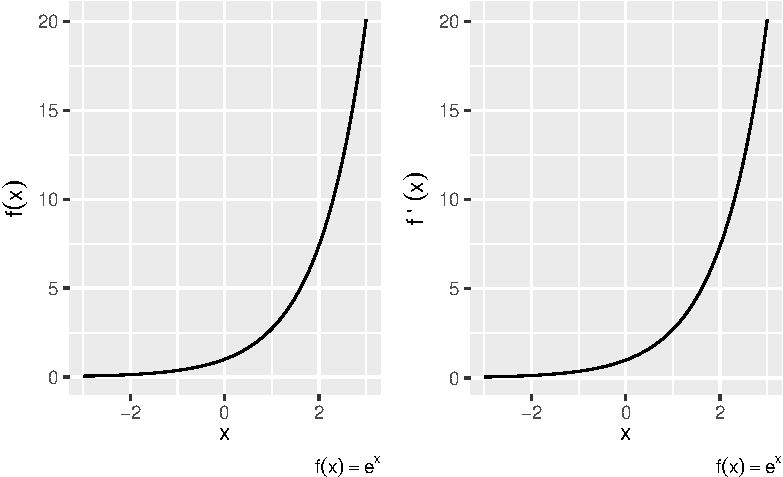
\includegraphics{./32_derivatives_files/figure-pdf/fig-derivexponent-1.pdf}

}

\caption{\label{fig-derivexponent}Derivative of the Exponential
Function}

\end{figure}

\leavevmode\vadjust pre{\hypertarget{exm-exmderivexp}{}}%
\begin{example}[]\label{exm-exmderivexp}

Find the derivative for the following.

\begin{enumerate}
\def\labelenumi{\arabic{enumi}.}
\tightlist
\item
  \(f(x)=e^{-3x}\)
\item
  \(f(x)=e^{x^2}\)
\item
  \(f(x)=(x-1)e^x\)
\end{enumerate}

\end{example}

\hypertarget{derivatives-of-logs}{%
\subsection*{Derivatives of logs}\label{derivatives-of-logs}}
\addcontentsline{toc}{subsection}{Derivatives of logs}

The natural log is the mirror image of the natural exponent and has
mirroring properties, again, to repeat the theorem,

\begin{enumerate}
\def\labelenumi{\arabic{enumi}.}
\tightlist
\item
  log prime x is one over x (Figure~\ref{fig-derivlog}):
\end{enumerate}

\[\frac{d}{dx} \ln x = \frac{1}{x}\]

\begin{enumerate}
\def\labelenumi{\arabic{enumi}.}
\setcounter{enumi}{1}
\tightlist
\item
  Exponents become multiplicative constants:
\end{enumerate}

\[\frac{d}{dx} \ln x^k = \frac{d}{dx} k \ln x = \frac{k}{x}\]

\begin{enumerate}
\def\labelenumi{\arabic{enumi}.}
\setcounter{enumi}{2}
\tightlist
\item
  Chain rule again:
\end{enumerate}

\[\frac{d}{dx} \ln u(x) = \frac{u'(x)}{u(x)}\quad\]

\begin{enumerate}
\def\labelenumi{\arabic{enumi}.}
\setcounter{enumi}{3}
\tightlist
\item
  For any positive base \(b\),
\end{enumerate}

\[\frac{d}{dx} b^x = (\ln b)\left(b^x\right)\]

\begin{figure}

{\centering 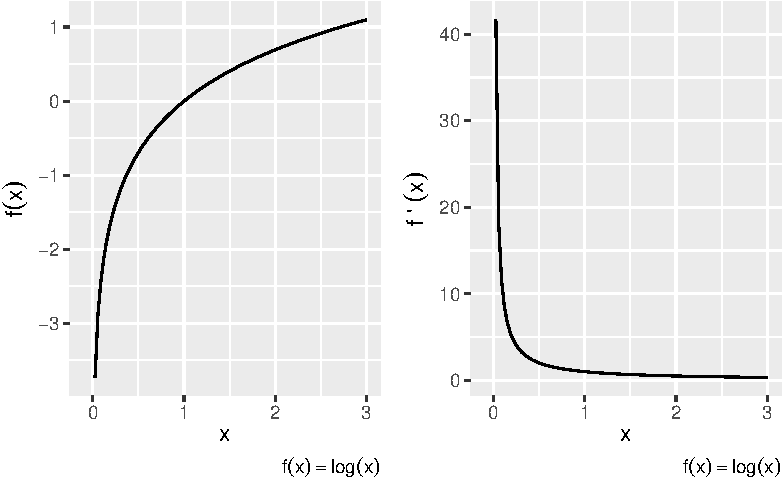
\includegraphics{./32_derivatives_files/figure-pdf/fig-derivlog-1.pdf}

}

\caption{\label{fig-derivlog}Derivative of the Natural Log}

\end{figure}

\leavevmode\vadjust pre{\hypertarget{exm-exmderivlog}{}}%
\begin{example}[]\label{exm-exmderivlog}

Find \(dy/dx\) for the following.

\begin{enumerate}
\def\labelenumi{\arabic{enumi}.}
\tightlist
\item
  \(f(x)=\ln(x^2+9)\)
\item
  \(f(x)=\ln(\ln x)\)
\item
  \(f(x)=(\ln x)^2\)
\item
  \(f(x)=\ln e^x\)
\end{enumerate}

\end{example}

\hypertarget{outline-of-proof}{%
\subsection*{Outline of Proof}\label{outline-of-proof}}
\addcontentsline{toc}{subsection}{Outline of Proof}

We actually show the derivative of the log first, and then the
derivative of the exponential naturally follows.

The general derivative of the log at any base \(a\) is solvable by the
definition of derivatives.

\begin{align*}
(\ln_a x)^\prime = \lim\limits_{h\to 0} \frac{1}{h}\ln_{a}\left(1 + \frac{h}{x}\right)
\end{align*}

Re-express \(g = \frac{h}{x}\) and get \begin{align*}
(\ln_a x)^\prime &= \frac{1}{x}\lim_{g\to 0}\ln_{a} (1 + g)^{\frac{1}{g}}\\
&= \frac{1}{x}\ln_a e
\end{align*}

By definition of \(e\). As a special case, when \(a = e\), then
\((\ln x)^\prime = \frac{1}{x}\).

Now let's think about the inverse, taking the derivative of \(y = a^x\).

\begin{align*}
y &= a^x \\
\Rightarrow \ln y &= x \ln a\\
\Rightarrow \frac{y^\prime}{y} &= \ln a\\
\Rightarrow  y^\prime = y \ln a\\
\end{align*}

Then in the special case where \(a = e\),

\[(e^x)^\prime = (e^x)\]

\hypertarget{partial-derivatives}{%
\section{Partial Derivatives}\label{partial-derivatives}}

What happens when there's more than variable that is changing?

\begin{quote}
If you can do ordinary derivatives, you can do partial derivatives: just
hold all the other input variables constant except for the one you're
differentiating with respect to. (Joe Blitzstein's Math Notes)
\end{quote}

Suppose we have a function \(f\) now of two (or more) variables and we
want to determine the rate of change relative to one of the variables.
To do so, we would find its partial derivative, which is defined similar
to the derivative of a function of one variable.

\textbf{Partial Derivative}: Let \(f\) be a function of the variables
\((x_1,\ldots,x_n)\). The partial derivative of \(f\) with respect to
\(x_i\) is

\[\frac{\partial f}{\partial x_i} (x_1,\ldots,x_n) = \lim\limits_{h\to 0} \frac{f(x_1,\ldots,x_i+h,\ldots,x_n)-f(x_1,\ldots,x_i,\ldots,x_n)}{h}\]

Only the \(i\)th variable changes --- the others are treated as
constants.

We can take higher-order partial derivatives, like we did with functions
of a single variable, except now the higher-order partials can be with
respect to multiple variables.

\leavevmode\vadjust pre{\hypertarget{exm-}{}}%
\begin{example}[]\label{exm-}

Notice that you can take partials with regard to different variables.

Suppose \(f(x,y)=x^2+y^2\). Then

\begin{align*}
\frac{\partial f}{\partial x}(x,y) &=\\
\frac{\partial f}{\partial y}(x,y) &=\\
\frac{\partial^2 f}{\partial x^2}(x,y) &=\\
\frac{\partial^2 f}{\partial x \partial y}(x,y) &=
\end{align*}

\end{example}

\leavevmode\vadjust pre{\hypertarget{exr-}{}}%
\begin{exercise}[]\label{exr-}

Let \(f(x,y)=x^3 y^4 +e^x -\ln y\). What are the following partial
derivaitves?

\begin{align*}
\frac{\partial f}{\partial x}(x,y) &=\\
\frac{\partial f}{\partial y}(x,y) &=\\
\frac{\partial^2 f}{\partial x^2}(x,y) &=\\
\frac{\partial^2 f}{\partial x \partial y}(x,y) &= 
\end{align*}

\end{exercise}

\hypertarget{taylorapprox}{%
\section{Taylor Approximation}\label{taylorapprox}}

A common form of approximation used in statistics involves derivatives.
A Taylor series is a way to represent common functions as infinite
series (a sum of infinite elements) of the function's derivatives at
some point \(a\).

For example, Taylor series are very helpful in representing nonlinear
(read: difficult) functions as linear (read: manageable) functions. One
can thus \textbf{approximate} functions by using lower-order, finite
series known as \textbf{Taylor polynomials}. If \(a=0\), the series is
called a Maclaurin series.

Specifically, a Taylor series of a real or complex function \(f(x)\)
that is infinitely differentiable in the neighborhood of point \(a\) is:

\begin{align*}
    f(x) &= f(a) + \frac{f'(a)}{1!} (x-a) +  \frac{f''(a)}{2!} (x-a)^2 + \cdots\\
     &= \sum_{n=0}^\infty \frac{f^{(n)} (a)}{n!} (x-a)^n
\end{align*}

\textbf{Taylor Approximation}: We can often approximate the curvature of
a function \(f(x)\) at point \(a\) using a 2nd order Taylor polynomial
around point \(a\):

\[f(x) = f(a) + \frac{f'(a)}{1!} (x-a) +  \frac{f''(a)}{2!} (x-a)^2 + R_2\]

\(R_2\) is the remainder (R for remainder, 2 for the fact that we took
two derivatives) and often treated as negligible, giving us:

\[f(x) \approx f(a) + f'(a)(x-a) +  \dfrac{f''(a)}{2} (x-a)^2\]

The more derivatives that are added, the smaller the remainder \(R\) and
the more accurate the approximation. Proofs involving limits guarantee
that the remainder converges to 0 as the order of derivation increases.

\hypertarget{optim}{%
\chapter{Optimization}\label{optim}}

To optimize, we use derivatives and calculus. Optimization is to find
the maximum or minimum of a functon, and to find what value of an input
gives that extremum. This has obvious uses in engineering. Many tools in
the statistical toolkit use optimization. One of the most common ways of
estimating a model is through ``Maximum Likelihood Estimation'', done
via optimizing a function (the likelihood).

Optimization also comes up in Economics, Formal Theory, and Political
Economy all the time. A go-to model of human behavior is that they
optimize a certain utility function. Humans are not pure utility
maximizers, of course, but nuanced models of optimization -- for
example, adding constraints and adding uncertainty -- will prove to be
quite useful.

\hypertarget{maxima-and-minima}{%
\section{Maxima and Minima}\label{maxima-and-minima}}

The first derivative, \(f'(x)\), quantifies the slope of a function.
Therefore, it can be used to check whether the function \(f(x)\) at the
point \(x\) is increasing or decreasing at \(x\).

\begin{enumerate}
\def\labelenumi{\arabic{enumi}.}
\tightlist
\item
  \textbf{Increasing:} \(f'(x)>0\)
\item
  \textbf{Decreasing:} \(f'(x)<0\)
\item
  \textbf{Neither increasing nor decreasing}: \(f'(x)=0\) i.e.~a
  maximum, minimum, or saddle point
\end{enumerate}

So for example, \(f(x) = x^2 + 2\) and \(f^\prime(x) = 2x\)

\begin{figure}

{\centering \includegraphics{./33_optimization_files/figure-pdf/unnamed-chunk-2-1.pdf}

}

\caption{Maxima and Minima}

\end{figure}

\leavevmode\vadjust pre{\hypertarget{exr-}{}}%
\begin{exercise}[Plotting a mazimum and minimum]\label{exr-}

Plot \(f(x)=x^3+ x^2 + 2\), plot its derivative, and identifiy where the
derivative is zero. Is there a maximum or minimum?

\end{exercise}

The second derivative \(f''(x)\) identifies whether the function
\(f(x)\) at the point \(x\) is

\begin{enumerate}
\def\labelenumi{\arabic{enumi}.}
\tightlist
\item
  Concave / concave down: \(f''(x)<0\)
\item
  Convex / Concave up: \(f''(x)>0\)
\end{enumerate}

\textbf{Maximum (Minimum)}: \(x_0\) is a \textbf{local maximum
(minimum)} if \(f(x_0)>f(x)\) (\(f(x_0)<f(x))\) for all \(x\) within
some open interval containing \(x_0\). \(x_0\) is a \textbf{global
maximum (minimum)} if \(f(x_0)>f(x)\) (\(f(x_0)<f(x))\) for all \(x\) in
the domain of \(f\).

Given the function \(f\) defined over domain \(D\), all of the following
are defined as \textbf{critical points}:

\begin{enumerate}
\def\labelenumi{\arabic{enumi}.}
\tightlist
\item
  Any interior point of \(D\) where \(f'(x)=0\).
\item
  Any interior point of \(D\) where \(f'(x)\) does not exist.
\item
  Any endpoint that is in \(D\).
\end{enumerate}

The maxima and minima will be a subset of the critical points.

\textbf{Second Derivative Test of Maxima/Minima}: We can use the second
derivative to tell us whether a point is a maximum or minimum of
\(f(x)\).

\begin{enumerate}
\def\labelenumi{\arabic{enumi}.}
\tightlist
\item
  Local Maximum: \(f'(x)=0\) and \(f''(x)<0\)
\item
  Local Minimum: \(f'(x)=0\) and \(f''(x)>0\)
\item
  Need more info: \(f'(x)=0\) and \(f''(x)=0\)
\end{enumerate}

\textbf{Global Maxima and Minima} Sometimes no global max or min exists
--- e.g., \(f(x)\) not bounded above or below. However, there are three
situations where we can fairly easily identify global max or min.

\begin{enumerate}
\def\labelenumi{\arabic{enumi}.}
\tightlist
\item
  \textbf{Functions with only one critical point.} If \(x_0\) is a local
  max or min of \(f\) and it is the only critical point, then it is the
  global max or min.
\item
  \textbf{Globally concave up or concave down functions.} If \(f''(x)\)
  is never zero, then there is at most one critical point. That critical
  point is a global maximum if \(f''<0\) and a global minimum if
  \(f''>0\).
\item
  \textbf{Functions over closed and bounded intervals} must have both a
  global maximum and a global minimum.
\end{enumerate}

\leavevmode\vadjust pre{\hypertarget{exm-}{}}%
\begin{example}[Maxima and Minima by drawing]\label{exm-}

Find any critical points and identify whether they are a max, min, or
saddle point:

\begin{enumerate}
\def\labelenumi{\arabic{enumi}.}
\tightlist
\item
  \(f(x)=x^2+2\)
\item
  \(f(x)=x^3+2\)
\item
  \(f(x)=|x^2-1|\), \(x\in [-2,2]\)
\end{enumerate}

\end{example}

\hypertarget{concavity-of-a-function}{%
\section{Concavity of a Function}\label{concavity-of-a-function}}

Concavity helps identify the curvature of a function, \(f(x)\), in 2
dimensional space.

\leavevmode\vadjust pre{\hypertarget{def-}{}}%
\begin{definition}[Concave Function]\label{def-}

A function \(f\) is strictly concave over the set S \underline{if}
\(\forall x_1,x_2 \in S\) and \(\forall a \in (0,1)\),
\[f(ax_1 + (1-a)x_2) > af(x_1) + (1-a)f(x_2)\] \textit{Any} line
connecting two points on a concave function will lie \textit{below} the
function.

\end{definition}

\includegraphics{./33_optimization_files/figure-pdf/unnamed-chunk-4-1.pdf}

\leavevmode\vadjust pre{\hypertarget{def-}{}}%
\begin{definition}[Convex Function]\label{def-}

Convex: A function f is strictly convex over the set S \underline{if}
\(\forall x_1,x_2 \in S\) and \(\forall a \in (0,1)\),
\[f(ax_1 + (1-a)x_2) < af(x_1) + (1-a)f(x_2)\]

Any line connecting two points on a convex function will lie above the
function.

\end{definition}

\textbf{Second Derivative Test of Concavity}: The second derivative can
be used to understand concavity.

If

\[\left\{\begin{array}{lll}
f''(x) < 0 & \Rightarrow & \text{Concave}\\
f''(x) > 0 & \Rightarrow & \text{Convex}
\end{array}\right.\]

\hypertarget{quadratic-forms}{%
\subsection*{Quadratic Forms}\label{quadratic-forms}}
\addcontentsline{toc}{subsection}{Quadratic Forms}

Quadratic forms is shorthand for a way to summarize a function. This is
important for finding concavity because

\begin{enumerate}
\def\labelenumi{\arabic{enumi}.}
\tightlist
\item
  Approximates local curvature around a point --- e.g., used to identify
  max vs min vs saddle point.
\item
  They are simple to express even in \(n\) dimensions:
\item
  Have a matrix representation.
\end{enumerate}

\textbf{Quadratic Form}: A polynomial where each term is a monomial of
degree 2 in any number of variables:

\begin{align*}
\text{One variable: }& Q(x_1) = a_{11}x_1^2\\
\text{Two variables: }& Q(x_1,x_2) = a_{11}x_1^2 + a_{12}x_1x_2 + a_{22}x_2^2\\
\text{N variables: }& Q(x_1,\cdots,x_n)=\sum\limits_{i\le j} a_{ij}x_i x_j
\end{align*}

which can be written in matrix terms:

One variable

\[Q(\mathbf{x}) = x_1^\top a_{11} x_1\]

N variables: \begin{align*}
Q(\mathbf{x}) &=\begin{bmatrix} x_1 & x_2 & \cdots & x_n \end{bmatrix}\begin{bmatrix}
a_{11}&\frac{1}{2}a_{12}&\cdots&\frac{1}{2}a_{1n}\\
\frac{1}{2}a_{12}&a_{22}&\cdots&\frac{1}{2}a_{2n}\\
\vdots&\vdots&\ddots&\vdots\\
\frac{1}{2}a_{1n}&\frac{1}{2}a_{2n}&\cdots&a_{nn}
\end{bmatrix}
\begin{bmatrix} x_1\\x_2\\\vdots\\x_n\end{bmatrix}\\
&= \mathbf{x}^\top\mathbf{Ax}
\end{align*}

For example, the Quadratic on \(\mathbb{R}^2\): \begin{align*}
  Q(x_1,x_2)&=\begin{bmatrix} x_1& x_2 \end{bmatrix} \begin{bmatrix} a_{11}&\frac{1}{2} a_{12}\\
  \frac{1}{2}a_{12}&a_{22}\end{bmatrix} \begin{bmatrix} x_1\\x_2 \end{bmatrix} \\
  &= a_{11}x_1^2 + a_{12}x_1x_2 + a_{22}x_2^2
\end{align*}

\hypertarget{definiteness-of-quadratic-forms}{%
\subsection*{Definiteness of Quadratic
Forms}\label{definiteness-of-quadratic-forms}}
\addcontentsline{toc}{subsection}{Definiteness of Quadratic Forms}

When the function \(f(\mathbf{x})\) has more than two inputs,
determining whether it has a maxima and minima (remember, functions may
have many inputs but they have only one output) is a bit more tedious.
Definiteness helps identify the curvature of a function,
\(Q(\textbf{x})\), in n dimensional space.

\textbf{Definiteness}: By definition, a quadratic form always takes on
the value of zero when \(x = 0\), \(Q(\textbf{x})=0\) at
\(\textbf{x}=0\). The definiteness of the matrix \(\textbf{A}\) is
determined by whether the quadratic form
\(Q(\textbf{x})=\textbf{x}^\top\textbf{A}\textbf{x}\) is greater than
zero, less than zero, or sometimes both over all \(\mathbf{x}\ne 0\).

\hypertarget{gradient-and-foc}{%
\section{Gradient and FOC}\label{gradient-and-foc}}

We can see from a graphical representation that if a point is a local
maxima or minima, it must meet certain conditions regarding its
derivative. These are so commonly used that we refer these to ``First
Order Conditions'' (FOCs) and ``Second Order Conditions'' (SOCs) in the
economic tradition.

When we examined functions of one variable \(x\), we found critical
points by taking the first derivative, setting it to zero, and solving
for \(x\). For functions of \(n\) variables, the critical points are
found in much the same way, except now we set the partial derivatives
equal to zero. Note: We will only consider critical points on the
interior of a function's domain.

In a derivative, we only took the derivative with respect to one
variable at a time. When we take the derivative separately with respect
to all variables in the elements of \(\mathbf{x}\) and then express the
result as a vector, we use the term Gradient and Hessian.

\leavevmode\vadjust pre{\hypertarget{def-}{}}%
\begin{definition}[Gradient]\label{def-}

Given a function \(f(\textbf{x})\) in \(n\) variables, the gradient
\(\nabla f(\mathbf{x})\) (the greek letter nabla ) is a row vector,
where the \(i\)th element is the partial derivative of \(f(\textbf{x})\)
with respect to \(x_i\):

\[\nabla f(\mathbf{x}) = \begin{bmatrix} \frac{\partial f(\mathbf{x})}{\partial x_1} &  \frac{\partial f(\mathbf{x})}{\partial x_2} & \cdots & \frac{\partial f(\mathbf{x})}{\partial x_n} \end{bmatrix}\]

\end{definition}

The gradient points in the direction of the steepest rate of increase at
each point \(\mathbf{x}\).

Before we know whether a point is a maxima or minima, if it meets the
FOC it is a ``Critical Point''.

\leavevmode\vadjust pre{\hypertarget{def-}{}}%
\begin{definition}[Critical Point]\label{def-}

\(\mathbf{x}^*\) is a critical point if and only if
\(\nabla f(\mathbf{x}^*)=\mathbf{0}\) (the vector of zeros). If the
partial derivative of f(x) with respect to \(x^*\) is 0, then
\(\mathbf{x}^*\) is a critical point. To solve for \(\mathbf{x}^*\),
find the gradient, set each element equal to 0, and solve the system of
equations.
\[\mathbf{x}^* = \begin{bmatrix} x_1^*\\x_2^*\\ \vdots \\ x_n^*\end{bmatrix}\]

\end{definition}

\leavevmode\vadjust pre{\hypertarget{exm-}{}}%
\begin{example}[]\label{exm-}

Example: Given a function \(f(\mathbf{x})=(x_1-1)^2+x_2^2+1\), find the
(1) Gradient and (2) Critical point of \(f(\mathbf{x})\).

\end{example}

\begin{solution}

Gradient

\begin{align*}
\nabla f(\mathbf{x}) &= 
  \begin{bmatrix}
  \frac{\partial f(\mathbf{x})}{\partial x_1} & 
  \frac{\partial f(\mathbf{x})}{\partial x_2} 
  \end{bmatrix}
  = 
  \begin{bmatrix} 2(x_1-1) &
  2x_2 
  \end{bmatrix}
\end{align*}

Critical Point \(\mathbf{x}^*\):

\begin{align*}
&\frac{\partial f(\mathbf{x})}{\partial x_1} = 2(x_1-1) = 0 & \Rightarrow x_1^* = 1\\
&\frac{\partial f(\mathbf{x})}{\partial x_2} = 2x_2 = 0 & \Rightarrow   x_2^* = 0\\
\end{align*}

So \[\mathbf{x}^* = (1,0)\]

\end{solution}

\hypertarget{hessian-and-soc}{%
\section{Hessian and SOC}\label{hessian-and-soc}}

When we found a critical point for a function of one variable, we used
the second derivative as a indicator of the curvature at the point in
order to determine whether the point was a min, max, or saddle (second
derivative test of concavity). For functions of \(n\) variables, we use
\emph{second order partial derivatives} as an indicator of curvature.

\leavevmode\vadjust pre{\hypertarget{def-}{}}%
\begin{definition}[Hessian]\label{def-}

Given a function \(f(\mathbf{x})\) in \(n\) variables, the hessian
\(\mathbf{H(x)}\) is an \(n\times n\) matrix, where the \((i,j)\)th
element is the second order partial derivative of \(f(\mathbf{x})\) with
respect to \(x_i\) and \(x_j\):

\[\mathbf{H(x)}=\begin{bmatrix} \frac{\partial^2 f(\mathbf{x})}{\partial x_1^2}&\frac{\partial^2f(\mathbf{x})}{\partial x_1 \partial x_2}& \cdots & \frac{\partial^2 f(\mathbf{x})}{\partial x_1 \partial x_n}\\ \frac{\partial^2 f(\mathbf{x})}{\partial x_2 \partial x_1}&\frac{\partial^2f(\mathbf{x})}{\partial x_2^2}& \cdots & \frac{\partial^2 f(\mathbf{x})}{\partial x_2 \partial x_n}\\ \vdots & \vdots & \ddots & \vdots \\ \frac{\partial^2 f(\mathbf{x})}{\partial x_n \partial x_1}&\frac{\partial^2f(\mathbf{x})}{\partial x_n \partial x_2}& \cdots & \frac{\partial^2 f(\mathbf{x})}{\partial x_n^2} \end{bmatrix}\]

\end{definition}

Note that the hessian will be a symmetric matrix because
\(\frac{\partial f(\mathbf{x})}{\partial x_1\partial x_2} = \frac{\partial f(\mathbf{x})}{\partial x_2\partial x_1}\).

Also note that given that \(f(\mathbf{x})\) is of quadratic form, each
element of the hessian will be a constant.

These definitions will be employed when we determine the \textbf{Second
Order Conditions} of a function:

Given a function \(f(\mathbf{x})\) and a point \(\mathbf{x}^*\) such
that \(\nabla f(\mathbf{x}^*)=0\),

\begin{enumerate}
\def\labelenumi{\arabic{enumi}.}
\tightlist
\item
  Hessian is Positive Definite around \(\mathbf{x}^*\)
  \(\quad \Longrightarrow \quad\) Local Min
\item
  Hessian is Negative Definite around \(\mathbf{x}^*\)
  \(\quad \Longrightarrow \quad\) Local Max
\item
  Hessian is Indefinite around \(\mathbf{x}^*\)
  \(\quad \Longrightarrow \quad\) Saddle Point
\end{enumerate}

Furthermore, there's an easier way to check whether a \(2\times 2\)
matrix is positive or negative definite.

\textbf{Definiteness of 2 \(\times\) 2 Matrix}: For a \(2 \times 2\)
matrix \$\$\mathbf{A}=

\begin{bmatrix}
A_{11} & A_{12}\\
A_{21} & A_{22}
\end{bmatrix}

\$\$

\begin{enumerate}
\def\labelenumi{\arabic{enumi}.}
\tightlist
\item
  If \(\mathrm{det}(\mathbf{A}) > 0\) and \(A_{11}>0\), then
  \(\mathbf{A}\) is positive definite
\item
  If \(\mathrm{det}(\mathbf{A}) > 0\) and \(A_{11}<0\), then
  \(\mathbf{A}\) is negative definite
\item
  If \(\mathrm{det}(\mathbf{A}) < 0\), then \(\mathbf{A}\) is indefinite
\end{enumerate}

\leavevmode\vadjust pre{\hypertarget{exm-}{}}%
\begin{example}[Max and min with two dimensions]\label{exm-}

We found that the only critical point of
\(f(\mathbf{x})=(x_1-1)^2+x_2^2+1\) is at \(\mathbf{x}^*=(1,0)\). Is it
a min, max, or saddle point?

\end{example}

\begin{solution}

The Hessian is \begin{align*}
\mathbf{H(x)} &= \begin{bmatrix} 2&0\\0&2 \end{bmatrix}
\end{align*} Since \(\mathrm{det}(\mathbf{H}(x)) = 4 > 0\) and
\(H_{11}=2>0\), the Hessian is positive definite.

Maxima, Minima, or Saddle Point? Since the Hessian is positive definite
and the gradient equals 0, \(x^\star = (1,0)\) is a local minimum.

Note: Alternate check of definiteness. Is
\(\mathbf{H(x^*)} \geq \leq 0 \quad \forall \quad \mathbf{x}\ne 0\)

\begin{align*}
\mathbf{x}^\top H(\mathbf{x}^*) \mathbf{x} &= \begin{bmatrix} x_1 & x_2 \end{bmatrix}\\
&= \begin{bmatrix} 2&0\\0&2 \end{bmatrix}\\
\begin{bmatrix} x_1\\x_2\end{bmatrix} &= 2x_1^2+2x_2^2
\end{align*}

For any \(\mathbf{x}\ne 0\), \(2(x_1^2+x_2^2)>0\), so the Hessian is
positive definite and \(\mathbf{x}^*\) is a strict local minimum.

\end{solution}

\hypertarget{definiteness-and-concavity}{%
\subsection*{Definiteness and
Concavity}\label{definiteness-and-concavity}}
\addcontentsline{toc}{subsection}{Definiteness and Concavity}

Although definiteness helps us to understand the curvature of an
n-dimensional function, it does not necessarily tell us whether the
function is globally concave or convex.

We need to know whether a function is globally concave or convex to
determine whether a critical point is a global min or max. We can use
the definiteness of the Hessian to determine whether a function is
globally concave or convex:

\begin{enumerate}
\def\labelenumi{\arabic{enumi}.}
\tightlist
\item
  Hessian is Positive Semidefinite \(\forall \mathbf{x}\)
  \(\quad \Longrightarrow \quad\) Globally Convex
\item
  Hessian is Negative Semidefinite \(\forall \mathbf{x}\)
  \(\quad \Longrightarrow \quad\) Globally Concave
\end{enumerate}

Notice that the definiteness conditions must be satisfied over the
entire domain.

\hypertarget{global-maxima-and-minima}{%
\section{Global Maxima and Minima}\label{global-maxima-and-minima}}

\textbf{Global Max/Min Conditions}: Given a function \(f(\mathbf{x})\)
and a point \(\mathbf{x}^*\) such that \(\nabla f(\mathbf{x}^*)=0\),

\begin{enumerate}
\def\labelenumi{\arabic{enumi}.}
\tightlist
\item
  \(f(\mathbf{x})\) Globally Convex \(\quad \Longrightarrow \quad\)
  Global Min
\item
  \(f(\mathbf{x})\) Globally Concave \(\quad \Longrightarrow \quad\)
  Global Max
\end{enumerate}

Note that showing that \(\mathbf{H(x^*)}\) is negative semidefinite is
not enough to guarantee \(\mathbf{x}^*\) is a local max. However,
showing that \(\mathbf{H(x)}\) is negative semidefinite for all
\(\mathbf{x}\) guarantees that \(x^*\) is a global max. (The same goes
for positive semidefinite and minima.)

\leavevmode\vadjust pre{\hypertarget{exm-}{}}%
\begin{example}[]\label{exm-}

Take \(f_1(x)=x^4\) and \(f_2(x)=-x^4\).

\begin{itemize}
\tightlist
\item
  Both have \(x=0\) as a critical point.\\
\item
  Unfortunately, \(f''_1(0)=0\) and \(f''_2(0)=0\), so we can't tell
  whether \(x=0\) is a min or max for either. However,
  \(f''_1(x)=12x^2\) and \(f''_2(x)=-12x^2\).\\
\item
  For all \(x\), \(f''_1(x)\ge 0\) and \(f''_2(x)\le 0\) --- i.e.,
  \(f_1(x)\) is globally convex and \(f_2(x)\) is globally concave.
\item
  So \(x=0\) is a global min of \(f_1(x)\) and a global max of
  \(f_2(x)\).
\end{itemize}

\end{example}

\leavevmode\vadjust pre{\hypertarget{exr-}{}}%
\begin{exercise}[]\label{exr-}

Given \(f(\mathbf{x})=x_1^3-x_2^3+9x_1x_2\), find any maxima or minima.

\end{exercise}

\emph{Solution.}

\begin{enumerate}
\def\labelenumi{\arabic{enumi}.}
\tightlist
\item
  First order conditions

  \begin{enumerate}
  \def\labelenumii{(\arabic{enumii})}
  \tightlist
  \item
    Gradient \(\nabla f(\mathbf{x})\)
    \[\begin{bmatrix} \frac{\partial f}{\partial x_1} \\ 
    \frac{\partial f}{\partial x_2}\end{bmatrix} =
    \begin{bmatrix} 3x_1^2+9x_2 \\ -3x_2^2+9x_1 \end{bmatrix}\]
  \item
    Critical Points \(\mathbf{x^*}\)

    \begin{itemize}
    \tightlist
    \item
      Set the gradient equal to zero and solve for \(x_1\) and \(x_2\).
      We have two equations and two unknowns. Solving for \(x_1\) and
      \(x_2\), we get two critical points: \(\mathbf{x}_1^*=(0,0)\) and
      \(\mathbf{x}_2^*=(3,-3)\).
    \item
      \(3x_1^2 + 9x_2 = 0 \quad \Rightarrow \quad 9x_2 = -3x_1^2 \quad \Rightarrow \quad x_2 = -\frac{1}{3}x_1^2\)
    \item
      \(-3x_2^2 + 9x_1 = 0 \quad \Rightarrow \quad -3(-\frac{1} {3}x_1^2)^2 + 9x_1 = 0\)
    \item
      \(\Rightarrow \quad -\frac{1}{3}x_1^4 + 9x_1 = 0 \quad \Rightarrow \quad x_1^3 = 27x_1 \quad \Rightarrow \quad x_1 = 3\)
    \item
      \(3(3)^2 + 9x_2 = 0 \quad \Rightarrow \quad x_2 = -3\)
    \end{itemize}
  \end{enumerate}
\item
  Second order conditions.

  \begin{enumerate}
  \def\labelenumii{(\arabic{enumii})}
  \item
    Hessian \(\mathbf{H(x)}\)

    \[\begin{bmatrix} 6x_1&9\\9&-6x_2 \end{bmatrix}\]
  \item
    Hessian \(\mathbf{H(x_1^*)}\)

    \[\begin{bmatrix} 0&9\\9&0\end{bmatrix}\]
  \item
    Leading principal minors of \(\mathbf{H(x_1^*)}\)

    \[M_1=0; M_2=-81\]
  \item
    Definiteness of \(\mathbf{H(x_1^*)}\)?

    \begin{itemize}
    \tightlist
    \item
      \(\mathbf{H(x_1^*)}\) is indefinite
    \end{itemize}
  \item
    Maxima, Minima, or Saddle Point for \(\mathbf{x_1^*}\)?

    \begin{itemize}
    \tightlist
    \item
      Since \(\mathbf{H(x_1^*)}\) is indefinite,
      \(\mathbf{x}_1^*=(0,0)\) is a saddle point.
    \end{itemize}
  \item
    Hessian

    \[\mathbf{H(x_2^*)}=\begin{bmatrix} 18&9\\9&18\end{bmatrix}\]
  \item
    Leading principal minors of \(\mathbf{H(x_2^*)}\)

    \[M_1=18; M_2=243\]
  \item
    Definiteness of \(\mathbf{H(x_2^*)}\)?

    \begin{itemize}
    \tightlist
    \item
      \(\mathbf{H(x_2^*)}\) is positive definite
    \end{itemize}
  \item
    Maxima, Minima, or Saddle Point for \(\mathbf{x}_2^*\)?

    \begin{itemize}
    \tightlist
    \item
      Since \(\mathbf{H(x_2^*)}\) is positive definite,
      \(\mathbf{x}_1^*=(3,-3)\) is a strict local minimum
    \end{itemize}
  \end{enumerate}
\item
  Global concavity/convexity.

  \begin{enumerate}
  \def\labelenumii{(\arabic{enumii})}
  \tightlist
  \item
    Is f(x) globally concave/convex?

    \begin{itemize}
    \tightlist
    \item
      No.~In evaluating the Hessians for \(\mathbf{x}_1^*\) and
      \(\mathbf{x}_2^*\) we saw that the Hessian is not positive
      semidefinite at x \(=\) (0,0).
    \end{itemize}
  \item
    Are any \(\mathbf{x^*}\) global minima or maxima?

    \begin{itemize}
    \tightlist
    \item
      No.~Since the function is not globally concave/convex, we can't
      infer that \(\mathbf{x}_2^*=(3,-3)\) is a global minimum. In fact,
      if we set \(x_1=0\), the \(f(\mathbf{x})=-x_2^3\), which will go
      to \(-\infty\) as \(x_2\to \infty\).
    \end{itemize}
  \end{enumerate}
\end{enumerate}

\hypertarget{integrals}{%
\chapter{Integral Calculus}\label{integrals}}

\hypertarget{the-indefinite-integral}{%
\section{The Indefinite Integral}\label{the-indefinite-integral}}

So far, we've been interested in finding the derivative \(f=F'\) of a
function \(F\). However, sometimes we're interested in exactly the
reverse: finding the function \(F\) for which \(f\) is its derivative.
We refer to \(F\) as the antiderivative of \(f\).

\leavevmode\vadjust pre{\hypertarget{def-}{}}%
\begin{definition}[Antiderivative]\label{def-}

The antiverivative of a function \(f(x)\) is a differentiable function
\(F\) whose derivative is \(f\).

\[F^\prime = f.\]

\end{definition}

Another way to describe is through the inverse formula. Let \(DF\) be
the derivative of \(F\). And let \(DF(x)\) be the derivative of \(F\)
evaluated at \(x\). Then the antiderivative is denoted by \(D^{-1}\)
(i.e., the inverse derivative). If \(DF=f\), then \(F=D^{-1}f\).

This definition bolsters the main takeaway about integrals and
derivatives: They are inverses of each other.

\leavevmode\vadjust pre{\hypertarget{exr-}{}}%
\begin{exercise}[Antiderivative]\label{exr-}

Find the antiderivative of the following:

\begin{enumerate}
\def\labelenumi{\arabic{enumi}.}
\tightlist
\item
  \(f(x) = \frac{1}{x^2}\)
\item
  \(f(x) = 3e^{3x}\)
\end{enumerate}

\end{exercise}

We know from derivatives how to manipulate \(F\) to get \(f\). But how
do you express the procedure to manipulate \(f\) to get \(F\)? For that,
we need a new symbol, which we will call indefinite integration.

\leavevmode\vadjust pre{\hypertarget{def-}{}}%
\begin{definition}[Indefinite Integral]\label{def-}

The indefinite integral of \(f(x)\) is written

\[\int f(x) dx \]

and is equal to the antiderivative of \(f\).

\end{definition}

\leavevmode\vadjust pre{\hypertarget{exm-}{}}%
\begin{example}[]\label{exm-}

Draw the function \(f(x)\) and its indefinite integral,
\(\int\limits f(x) dx\)

\[f(x) = (x^2-4)\]

\end{example}

\begin{solution}

The Indefinite Integral of the function \(f(x) = (x^2-4)\) can, for
example, be \(F(x) = \frac{1}{3}x^3 - 4x.\) But it can also be
\(F(x) = \frac{1}{3}x^3 - 4x + 1\), because the constant 1 disappears
when taking the derivative.

\end{solution}

Some of these functions are plotted in the bottom panel of
Figure~\ref{fig-integralc} as dotted lines.

\begin{figure}

{\centering 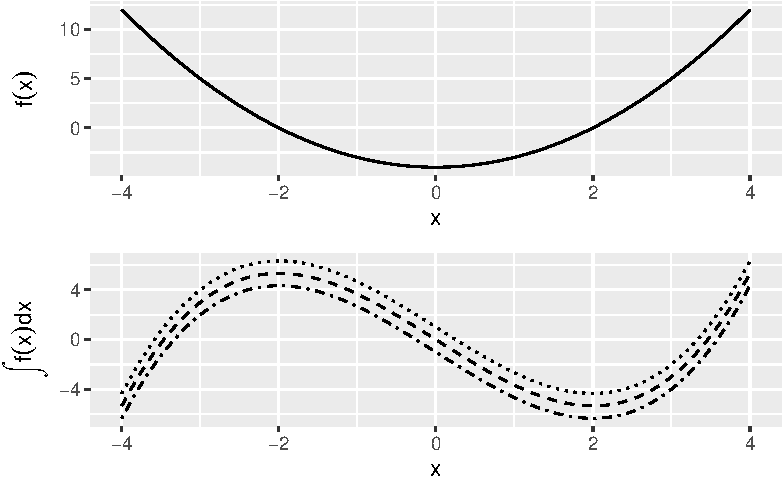
\includegraphics{./34_intergrals_files/figure-pdf/fig-integralc-1.pdf}

}

\caption{\label{fig-integralc}The Many Indefinite Integrals of a
Function}

\end{figure}

Notice from these examples that while there is only a single derivative
for any function, there are multiple antiderivatives: one for any
arbitrary constant \(c\). \(c\) just shifts the curve up or down on the
\(y\)-axis. If more information is present about the antiderivative ---
e.g., that it passes through a particular point --- then we can solve
for a specific value of \(c\).

\hypertarget{properties-of-integration}{%
\subsection*{Properties of
Integration}\label{properties-of-integration}}
\addcontentsline{toc}{subsection}{Properties of Integration}

Some useful properties of integrals follow by virtue of being the
inverse of a derivative.

\hypertarget{prop-}{}
\hypertarget{properties-of-integration-1}{%
\subsection{Properties of
Integration}\label{properties-of-integration-1}}

\begin{enumerate}
\def\labelenumi{\arabic{enumi}.}
\tightlist
\item
  Constants are allowed to slip out: \(\int a f(x)dx = a\int f(x)dx\)
\item
  Integration of the sum is sum of integrations:
  \(\int [f(x)+g(x)]dx=\int f(x)dx + \int g(x)dx\)
\item
  Reverse Power-rule: \(\int x^n dx = \frac{1}{n+1} x^{n+1} + c\)
\item
  Exponents are still exponents: \(\int e^x dx = e^x +c\)
\item
  Recall the derivative of \(\ln(x)\) is one over \(x\), and so:
  \(\int \frac{1}{x} dx = \ln x + c\)
\item
  Reverse chain-rule: \(\int e^{f(x)}f^\prime(x)dx = e^{f(x)}+c\)
\item
  More generally:
  \(\int [f(x)]^n f'(x)dx = \frac{1}{n+1}[f(x)]^{n+1}+c\)
\item
  Remember the derivative of a log of a function:
  \(\int \frac{f^\prime(x)}{f(x)}dx=\ln f(x) + c\)
\end{enumerate}

\leavevmode\vadjust pre{\hypertarget{exm-}{}}%
\begin{example}[Common Integration]\label{exm-}

Simplify the following indefinite integrals:

\begin{itemize}
\tightlist
\item
  \(\int 3x^2 dx\)
\item
  \(\int (2x+1)dx\)
\item
  \(\int e^x e^{e^x} dx\)
\end{itemize}

\end{example}

\hypertarget{the-definite-integral}{%
\section{The Definite Integral}\label{the-definite-integral}}

If there is a indefinite integral, there \emph{must} be a definite
integral. Indeed there is, but the notion of definite integrals comes
from a different objective: finding the are a under a function. We will
find, perhaps remarkably, that the formula we find to get the sum turns
out to be expressible by the anti-derivative.

Suppose we want to determine the area \(A(R)\) of a region \(R\) defined
by a curve \(f(x)\) and some interval \(a\le x \le b\).

\begin{figure}

{\centering 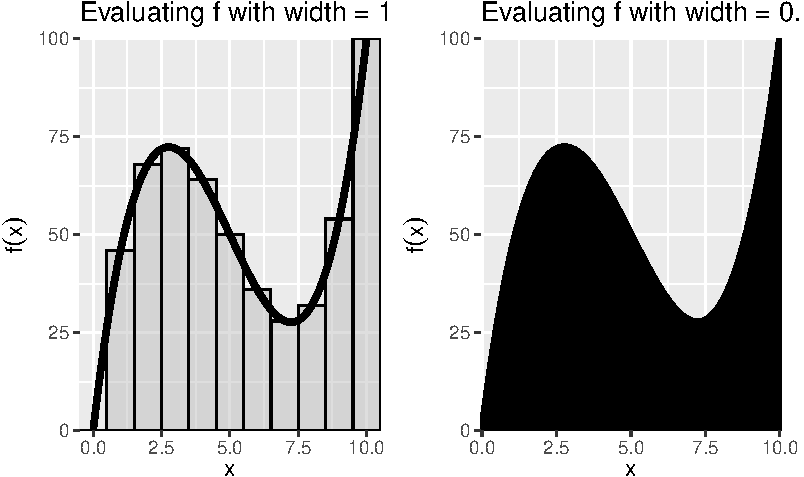
\includegraphics{./34_intergrals_files/figure-pdf/fig-defintfig-1.pdf}

}

\caption{\label{fig-defintfig}The Riemann Integral as a Sum of
Evaluations}

\end{figure}

One way to calculate the area would be to divide the interval
\(a\le x\le b\) into \(n\) subintervals of length \(\Delta x\) and then
approximate the region with a series of rectangles, where the base of
each rectangle is \(\Delta x\) and the height is \(f(x)\) at the
midpoint of that interval. \(A(R)\) would then be approximated by the
area of the union of the rectangles, which is given by
\[S(f,\Delta x)=\sum\limits_{i=1}^n f(x_i)\Delta x\] and is called a
\textbf{Riemann sum}.

As we decrease the size of the subintervals \(\Delta x\), making the
rectangles ``thinner,'' we would expect our approximation of the area of
the region to become closer to the true area. This allows us to express
the area as a limit of a series:

\[A(R)=\lim\limits_{\Delta x\to 0}\sum\limits_{i=1}^n f(x_i)\Delta x\]

Figure~\ref{fig-defintfig} shows that illustration. The curve depicted
is \(f(x) = -15(x - 5) + (x - 5)^3 + 50.\) We want approximate the area
under the curve between the \(x\) values of 0 and 10. We can do this in
blocks of arbitrary width, where the sum of rectangles (the area of
which is width times \(f(x)\) evaluated at the midpoint of the bar)
shows the Riemann Sum. As the width of the bars \(\Delta x\) becomes
smaller, the better the estimate of \(A(R)\).

This is how we define the ``Definite'' Integral:

\leavevmode\vadjust pre{\hypertarget{def-}{}}%
\begin{definition}[The Definite Integral (Riemann)]\label{def-}

If for a given function \(f\) the Riemann sum approaches a limit as
\(\Delta x \to 0\), then that limit is called the Riemann integral of
\(f\) from \(a\) to \(b\). We express this with the \(\int\), symbol,
and write
\[\int\limits_a^b f(x) dx= \lim\limits_{\Delta x\to 0} \sum\limits_{i=1}^n f(x_i)\Delta x\]

The most straightforward of a definite integral is the definite
integral. That is, we read

\[\int\limits_a^b f(x) dx\] as the definite integral of \(f\) from \(a\)
to \(b\) and we defined as the area under the ``curve'' \(f(x)\) from
point \(x=a\) to \(x=b\).

\end{definition}

The fundamental theorem of calculus shows us that this sum is, in fact,
the antiderivative.

\leavevmode\vadjust pre{\hypertarget{thm-}{}}%
\begin{theorem}[First Fundamental Theorem of Calculus]\label{thm-}

Let the function \(f\) be bounded on \([a,b]\) and continuous on
\((a,b)\). Then, suggestively, use the symbol \(F(x)\) to denote the
definite integral from \(a\) to \(x\)

\[F(x)=\int\limits_a^x f(t)dt, \quad a\le x\le b\]

Then \(F(x)\) has a derivative at each point in \((a,b)\) and
\[F^\prime(x)=f(x), \quad a<x<b\] That is, the definite integral
function of \(f\) \emph{is} the one of the antiderivatives of some
\(f\).

\end{theorem}

This is again a long way of saying that that differentiation is the
inverse of integration. But now, we've covered definite integrals.

The second theorem gives us a simple way of computing a definite
integral as a function of indefinite integrals.

\hypertarget{thm}{}
\hypertarget{second-fundamental-theorem-of-calculus}{%
\subsection{Second Fundamental Theorem of
Calculus}\label{second-fundamental-theorem-of-calculus}}

Let the function \(f\) be bounded on \([a,b]\) and continuous on
\((a,b)\). Let \(F\) be any function that is continuous on \([a,b]\)
such that \(F^\prime(x)=f(x)\) on \((a,b)\). Then
\[\int\limits_a^bf(x)dx = F(b)-F(a)\]

So the procedure to calculate a simple definite integral
\(\int\limits_a^b f(x)dx\) is then

\begin{enumerate}
\def\labelenumi{\arabic{enumi}.}
\tightlist
\item
  Find the indefinite integral \(F(x)\).
\item
  Evaluate \(F(b)-F(a)\).
\end{enumerate}

\leavevmode\vadjust pre{\hypertarget{exm-defintmon}{}}%
\begin{example}[Definite Integral of a monomial]\label{exm-defintmon}

Solve \(\int\limits_1^3 3x^2 dx.\) Let \(f(x) = 3x^2\).

\end{example}

\leavevmode\vadjust pre{\hypertarget{exr-}{}}%
\begin{exercise}[]\label{exr-}

What is the value of \(\int\limits_{-2}^2 e^x e^{e^x} dx\)?

\end{exercise}

\hypertarget{properties-for-definite-integrals}{%
\subsection*{Properties for Definite
Integrals}\label{properties-for-definite-integrals}}
\addcontentsline{toc}{subsection}{Properties for Definite Integrals}

The area-interpretation of the definite integral provides some useful
properties for definite integrals

\hypertarget{prop-}{}
\begin{enumerate}
\def\labelenumi{\arabic{enumi}.}
\tightlist
\item
  There is no area below a point: \[\int\limits_a^a f(x)dx=0\]
\item
  Reversing the limits changes the sign of the integral:
  \[\int\limits_a^b f(x)dx=-\int\limits_b^a f(x)dx\]
\item
  Sums can be separated into their own integrals:
  \[\int\limits_a^b [\alpha f(x)+\beta g(x)]dx = \alpha \int\limits_a^b f(x)dx + \beta \int\limits_a^b g(x)dx\]
\item
  Areas can be combined as long as limits are linked:
  \[\int\limits_a^b f(x) dx +\int\limits_b^c f(x)dx = \int\limits_a^c f(x)dx\]
\end{enumerate}

\leavevmode\vadjust pre{\hypertarget{exr-}{}}%
\begin{exercise}[]\label{exr-}

Simplify the following definite intergrals.

\begin{enumerate}
\def\labelenumi{\arabic{enumi}.}
\tightlist
\item
  \(\int\limits_1^1 3x^2 dx =\)
\item
  \(\int\limits_0^4 (2x+1)dx=\)
\item
  \(\int\limits_{-2}^0 e^x e^{e^x} dx + \int\limits_0^2 e^x e^{e^x} dx =\)
\end{enumerate}

\end{exercise}

\hypertarget{integration-by-substitution}{%
\section{Integration by
Substitution}\label{integration-by-substitution}}

From the second fundamental theorem of calculus, we now that a quick way
to get a definite integral is to first find the indefinite integral, and
then just plug in the bounds.

Sometimes the integrand (the thing that we are trying to take an
integral of) doesn't appear integrable using common rules and
antiderivatives. A method one might try is \textbf{integration by
substitution}, which is related to the Chain Rule.

Suppose we want to find the indefinite integral \[\int g(x)dx\] but
\(g(x)\) is complex and none of the formulas we have seen so far seem to
apply immediately. The trick is to come up with a \emph{new} function
\(u(x)\) such that \[g(x)=f[u(x)]u'(x).\]

Why does an introduction of yet another function end of simplifying
things? Let's refer to the antiderivative of \(f\) as \(F\). Then the
chain rule tells us that \[\frac{d}{dx} F[u(x)]=f[u(x)]u'(x)\]. So,
\(F[u(x)]\) is the antiderivative of \(g\). We can then write
\[\int g(x) dx= \int f[u(x)]u'(x)dx = \int \frac{d}{dx} F[u(x)]dx = F[u(x)]+c\]

To summarize, the procedure to determine the indefinite integral
\(\int g(x)dx\) by the method of substitution:

\begin{enumerate}
\def\labelenumi{\arabic{enumi}.}
\tightlist
\item
  Identify some part of \(g(x)\) that might be simplified by
  substituting in a single variable \(u\) (which will then be a function
  of \(x\)).
\item
  Determine if \(g(x)dx\) can be reformulated in terms of \(u\) and
  \(du\).
\item
  Solve the indefinite integral.
\item
  Substitute back in for \(x\)
\end{enumerate}

Substitution can also be used to calculate a definite integral. Using
the same procedure as above,
\[\int\limits_a^b g(x)dx=\int\limits_c^d f(u)du = F(d)-F(c)\] where
\(c=u(a)\) and \(d=u(b)\).

\leavevmode\vadjust pre{\hypertarget{exm-intsub1}{}}%
\begin{example}[Integration by Substitution I]\label{exm-intsub1}

Solve the indefinite integral \[\int x^2 \sqrt{x+1}dx.\]

\end{example}

For the above problem, we could have also used the substitution
\(u=\sqrt{x+1}\). Then \(x=u^2-1\) and \(dx=2u du\). Substituting these
in, we get \[\int x^2\sqrt{x+1}dx=\int (u^2-1)^2 u 2u du\] which when
expanded is again a polynomial and gives the same result as above.

Another case in which integration by substitution is is useful is with a
fraction.

\leavevmode\vadjust pre{\hypertarget{exm-intsub2}{}}%
\begin{example}[Integration by Substitutiton II]\label{exm-intsub2}

Simplify \[\int\limits_0^1 \frac{5e^{2x}}{(1+e^{2x})^{1/3}}dx.\]

\end{example}

\hypertarget{integration-by-parts}{%
\section{Integration by Parts}\label{integration-by-parts}}

Another useful integration technique is \textbf{integration by parts},
which is related to the Product Rule of differentiation. The product
rule states that \[\frac{d}{dx}(uv)=u\frac{dv}{dx}+v\frac{du}{dx}\]
Integrating this and rearranging, we get
\[\int u\frac{dv}{dx}dx= u v - \int v \frac{du}{dx}dx\] or
\[\int u(x) v'(x)dx=u(x)v(x) - \int v(x)u'(x)dx\]

More easily remembered with the mnemonic ``Ultraviolet Voodoo'':
\[\int u dv = u v - \int v du\] where \(du=u'(x)dx\) and \(dv=v'(x)dx\).

For definite integrals, this is simply

\[\int\limits_a^b u\frac{dv}{dx}dx = \left. u v \right|_a^b - \int\limits_a^b v \frac{du}{dx}dx\]

Our goal here is to find expressions for \(u\) and \(dv\) that, when
substituted into the above equation, yield an expression that's more
easily evaluated.

\leavevmode\vadjust pre{\hypertarget{exm-}{}}%
\begin{example}[Integration by Parts I]\label{exm-}

Simplify the following integrals. These seemingly obscure forms of
integrals come up often when integrating distributions.

\[\int x e^{ax} dx\]

\end{example}

\begin{solution}

Let \(u=x\) and \(\frac{dv}{dx} = e^{ax}\). Then \(du=dx\) and
\(v=(1/a)e^{ax}\). Substituting this into the integration by parts
formula, we obtain\\
\begin{align*}
\int x e^{ax} dx &= u v - \int v du\nonumber\\
                &=x\left( \frac{1}{a}e^{ax}\right) -\int\frac{1}{a}e^{ax}dx\nonumber\\
                &=\frac{1}{a}xe^{ax}-\frac{1}{a^2}e^{ax}+c\nonumber
\end{align*}

\end{solution}

\leavevmode\vadjust pre{\hypertarget{exr-intparts-adv}{}}%
\begin{exercise}[Integration by Parts II]\label{exr-intparts-adv}

\begin{enumerate}
\def\labelenumi{\arabic{enumi}.}
\tightlist
\item
  Integrate
\end{enumerate}

\[\int x^n e^{ax} dx\]

\begin{enumerate}
\def\labelenumi{\arabic{enumi}.}
\setcounter{enumi}{1}
\tightlist
\item
  Integrate
\end{enumerate}

\[\int x^3 e^{-x^2} dx\]

\end{exercise}

\hypertarget{answers-to-examples-and-exercises-2}{%
\section*{Answers to Examples and
Exercises}\label{answers-to-examples-and-exercises-2}}
\addcontentsline{toc}{section}{Answers to Examples and Exercises}

Exercise~\ref{exr-introderivatives}

\emph{Solution.}

\begin{enumerate}
\def\labelenumi{\arabic{enumi}.}
\tightlist
\item
  \(f^\prime(x)= 0\)
\item
  \(f^\prime(x)= 1\)
\item
  \(f^\prime(x)= 2x^3\)
\item
  \(f\prime(x)= 3x^2\)
\item
  \(f\prime(x)= -2x^{-3}\)
\item
  \(f\prime(x)= 14x^6\)
\item
  \(f\prime(x) = 4x^3 - 3x^2 + 2x -1\)
\item
  \(f\prime(x) = 5x^4 + 3x^2 - 2x\)
\item
  \(f\prime(x) = 6x + \frac{2}{3}x^{\frac{-2}{3}}\)
\item
  \(f\prime(x)= \frac{-4x}{x^4 - 2x^2 + 1}\)
\end{enumerate}

Example~\ref{exm-tothesix}

\begin{solution}

For convenience, define \(f(z) = z^6\) and \(z = g(x) = 3x^2+5x-7\).
Then, \(y=f[g(x)]\) and

\begin{align*}
\frac{d}{dx}y&= f^\prime(z) g^\prime(x) \\
&= 6(3x^2+5x-7)^5 (6x + 5)
\end{align*}

\end{solution}

Example~\ref{exm-exmderivexp}

\emph{Solution.}

\begin{enumerate}
\def\labelenumi{\arabic{enumi}.}
\tightlist
\item
  Let \(u(x)=-3x\). Then \(u^\prime(x)=-3\) and
  \(f^\prime(x)=-3e^{-3x}\).
\item
  Let \(u(x)=x^2\). Then \(u^\prime(x)=2x\) and
  \(f^\prime(x)=2xe^{x^2}\).
\end{enumerate}

Example~\ref{exm-exmderivlog}

\emph{Solution.}

\begin{enumerate}
\def\labelenumi{\arabic{enumi}.}
\tightlist
\item
  Let \(u(x)=x^2+9\). Then \(u^\prime(x)=2x\) and
  \[\frac{dy}{dx}= \frac{u^\prime(x)}{u(x)} = \frac{2x}{(x^2+9)}\]
\item
  Let \(u(x)=\ln x\). Then \(u^\prime(x)=1/x\) and
  \(\frac{dy}{dx} = \frac{1}{(x\ln x)}\).
\item
  Use the generalized power rule.
  \[\frac{dy}{dx} = \frac{(2 \ln x)}{x}\]
\item
  We know that \(\ln e^x=x\) and that \(dx/dx=1\), but we can double
  check. Let \(u(x)=e^x\). Then \(u^\prime(x)=e^x\) and
  \(\frac{dy}{dx} = \frac{u^\prime(x)}{u(x)} = \frac{e^x}{e^x} = 1.\)
\end{enumerate}

Example~\ref{exm-defintmon}

\begin{solution}

What is \(F(x)\)? From the power rule, recognize
\(\frac{d}{dx}x^3 = 3x^2\) so

\begin{align*}
F(x) &= x^3\\
\int\limits_1^3 f(x) dx &= F(x = 3) - F(x  - 1)\\
&= 3^3 - 1^3\\
&=26
\end{align*}

\end{solution}

Example~\ref{exm-intsub1}

\begin{solution}

The problem here is the \(\sqrt{x+1}\) term. However, if the integrand
had \(\sqrt{x}\) times some polynomial, then we'd be in business. Let's
try \(u=x+1\). Then \(x=u-1\) and \(dx=du\). Substituting these into the
above equation, we get

\begin{align*}
            \int x^2\sqrt{x+1}dx&= \int (u-1)^2\sqrt{u}du\\
            &= \int (u^2-2u+1)u^{1/2}du\\
            &= \int (u^{5/2}-2u^{3/2}+u^{1/2})du
\end{align*}

We can easily integrate this, since it is just a polynomial. Doing so
and substituting \(u=x+1\) back in, we get
\[\int x^2\sqrt{x+1}dx=2(x+1)^{3/2}\left[\frac{1}{7}(x+1)^2 -
\frac{2}{5}(x+1)+\frac{1}{3}\right]+c\]

\end{solution}

Example~\ref{exm-intsub2}

\begin{solution}

When an expression is raised to a power, it is often helpful to use this
expression as the basis for a substitution. So, let \(u=1+e^{2x}\). Then
\(du=2e^{2x}dx\) and we can set \(5e^{2x}dx=5du/2\). Additionally,
\(u=2\) when \(x=0\) and \(u=1+e^2\) when \(x=1\). Substituting all of
this in, we get

\begin{align*}
\int\limits_0^1 \frac{5e^{2x}}{(1+e^{2x})^{1/3}}dx
            &= \frac{5}{2}\int\limits_2^{1+e^2}\frac{du}{u^{1/3}}\\
            &= \frac{5}{2}\int\limits_2^{1+e^2} u^{-1/3}du\\
            &= \left. \frac{15}{4} u^{2/3} \right|_2^{1+e^2}\\
            &= 9.53
\end{align*}

\end{solution}

Exercise~\ref{exr-intparts-adv}

\emph{Solution.}

\begin{enumerate}
\def\labelenumi{\arabic{enumi}.}
\tightlist
\item
  \[\int x^n e^{ax} dx\]
\end{enumerate}

As in the first problem, let

\[u=x^n, dv=e^{ax}dx\]

Then \(du=n x^{n-1}dx\) and \(v=(1/a)e^{ax}\).

Substituting these into the integration by parts formula gives
\begin{align*}
    \int x^n e^{ax} dx &= u v - \int v du\nonumber\\
    &=x^n\left( \frac{1}{a}e^{ax}\right) - \int\frac{1}{a}e^{ax} n x^{n-1} dx\nonumber\\
    &=\frac{1}{a}x^n e^{ax} - \frac{n}{a}\int x^{n-1}e^{ax}dx\nonumber
\end{align*}

Notice that we now have an integral similar to the previous one, but
with \(x^{n-1}\) instead of \(x^n\).

For a given \(n\), we would repeat the integration by parts procedure
until the integrand was directly integratable --- e.g., when the
integral became \(\int e^{ax}dx\).

\begin{enumerate}
\def\labelenumi{\arabic{enumi}.}
\setcounter{enumi}{1}
\tightlist
\item
  \[\int x^3 e^{-x^2} dx\]
\end{enumerate}

We could, as before, choose \(u=x^3\) and \(dv=e^{-x^2}dx\). But we
can't then find \(v\) --- i.e., integrating \(e^{-x^2}dx\) isn't
possible. Instead, notice that \[\frac{d}{dx}e^{-x^2} = -2xe^{-x^2},\]
which can be factored out of the original integrand
\[\int x^3 e^{-x^2} dx = \int x^2 (xe^{-x^2})dx.\]

We can then let \(u=x^2\) and \(dv=x e^{-x^2}dx\). The\(du=2x dx\) and
\(v=-\frac{1}{2}e^{-x^2}\). Substituting these in, we have
\begin{align*}
    \int x^3 e^{-x^2} dx &= u v - \int v du\nonumber\\
    &= x^2 \left( -\frac{1}{2}e^{-x^2}\right) -\int \left(-\frac{1}{2}e^{-x^2}\right)2x dx\nonumber\\
    &= -\frac{1}{2}x^2 e^{-x^2}+\int x e^{-x^2}dx\nonumber\\
    &= -\frac{1}{2}x^2 e^{-x^2}-\frac{1}{2}e^{-x^2}+c\nonumber
\end{align*}

\part{IV Probability}

\hypertarget{probability-theory}{%
\chapter{Probability Theory}\label{probability-theory}}

Probability and Inferences are mirror images of each other, and both are
integral to social science. Probability quantifies uncertainty, which is
important because many things in the social world are at first
uncertain. Inference is then the study of how to learn about facts you
don't observe from facts you do observe.

\hypertarget{counting-rules}{%
\section{Counting Rules}\label{counting-rules}}

Probability in high school is usually really about combinatorics: the
probability of event \emph{A} is the number of ways in which \emph{A}
can occur divided by the number of all other possibilities. This is a
very simplified version of probability, which we can call the ``counting
definition of probability'', essentially because each possible event to
count is often equally likely and discrete. But it is still good to
review the underlying rules here.

\textbf{Fundamental Theorem of Counting}: If an object has \(j\)
different characteristics that are independent of each other, and each
characteristic \(i\) has \(n_i\) ways of being expressed, then there are
\(\prod_{i = 1}^j n_i\) possible unique objects.

\leavevmode\vadjust pre{\hypertarget{exm-countingrules}{}}%
\begin{example}[]\label{exm-countingrules}

Suppose we are given a stack of cards. Cards can be either red or black
and can take on any of 13 values. There is only one of each color-number
combination. In this case,

\begin{enumerate}
\def\labelenumi{\arabic{enumi}.}
\item
  \(j =\)
\item
  \(n_{\text{color}} =\)
\item
  \(n_{\text{number}} =\)
\item
  Number of Outcomes \(=\)
\end{enumerate}

\end{example}

We often need to count the number of ways to choose a subset from some
set of possibilities. The number of outcomes depends on two
characteristics of the process: does the order matter and is replacement
allowed?

It is useful to think of any problem concretely, e.g.~through a
\textbf{sampling table}: If there are \(n\) objects which are numbered 1
to \(n\) and we select \(k < n\) of them, how many different outcomes
are possible?

If the order in which a given object is selected matters, selecting 4
numbered objects in the following order (1, 3, 7, 2) and selecting the
same four objects but in a different order such as (7, 2, 1, 3) will be
counted as different outcomes.

If replacement is allowed, there are always the same \(n\) objects to
select from. However, if replacement is not allowed, there is always one
less option than the previous round when making a selection. For
example, if replacement is not allowed and I am selecting 3 elements
from the following set \{1, 2, 3, 4, 5, 6\}, I will have 6 options at
first, 5 options as I make my second selection, and 4 options as I make
my third.

\begin{enumerate}
\def\labelenumi{\arabic{enumi}.}
\item
  So if \textbf{\emph{order matters}} AND we are sampling
  \textbf{\emph{with replacement}}, the number of different outcomes is
  \(n^k\).
\item
  If \textbf{\emph{order matters}} AND we are sampling
  \textbf{\emph{without replacement}}, the number of different outcomes
  is \(n(n-1)(n-2)...(n-k+1)=\frac{n!}{(n-k)!}\).
\item
  If \textbf{\emph{order doesn't matter}} AND we are sampling
  \textbf{\emph{without replacement}}, the number of different outcomes
  is \(\binom{n}{k} = \frac{n!}{(n-k)!k!}\).
\end{enumerate}

Expression \(\binom{n}{k}\) is read as ``n choose k'' and denotes
\(\frac{n!}{(n-k)!k!}\). Also, note that \(0! = 1\).

\leavevmode\vadjust pre{\hypertarget{exm-counting}{}}%
\begin{example}[Counting]\label{exm-counting}

There are five balls numbered from 1 through 5 in a jar. Three balls are
chosen. How many possible choices are there?

\begin{enumerate}
\def\labelenumi{\arabic{enumi}.}
\item
  Ordered, with replacement \(=\)
\item
  Ordered, without replacement \(=\)
\item
  Unordered, without replacement \(=\)
\end{enumerate}

\end{example}

\leavevmode\vadjust pre{\hypertarget{exr-counting1}{}}%
\begin{exercise}[Counting]\label{exr-counting1}

Four cards are selected from a deck of 52 cards. Once a card has been
drawn, it is not reshuffled back into the deck. Moreover, we care only
about the complete hand that we get (i.e.~we care about the set of
selected cards, not the sequence in which it was drawn). How many
possible outcomes are there?

\end{exercise}

\hypertarget{setoper}{%
\section{Sets}\label{setoper}}

Probability is about quantifying the uncertainty of events. \emph{Sets}
(set theory) are the mathematical way we choose to formalize those
events. Events are not inherently numerical: the onset of war or the
stock market crashing is not inherently a number. Sets can define such
events, and we wrap math around so that we have a transparent language
to communicate about those events. \emph{Measure theory} might sound
mysterious or hard, but it is also just a mathematical way to quantify
things like length, volume, and mass. Probability can be thought of as a
particular application of measure theory where we want to quantify the
measure of a set.

\textbf{Set} : A set is any well defined collection of elements. If
\(x\) is an element of \(S\), \(x \in S\).

\textbf{Sample Space (S)}: A set or collection of all possible outcomes
from some process. Outcomes in the set can be discrete elements
(countable) or points along a continuous interval (uncountable).

Examples:

\begin{enumerate}
\def\labelenumi{\arabic{enumi}.}
\tightlist
\item
  Discrete: the numbers on a die, whether a vote cast is republican or
  democrat.
\item
  Continuous: GNP, arms spending, age.
\end{enumerate}

\textbf{Event}: Any collection of possible outcomes of an experiment.
Any subset of the full set of possibilities, including the full set
itself. Event A \(\subset\) S.

\textbf{Empty Set}: a set with no elements. \(S = \{\}\). It is denoted
by the symbol \(\emptyset\).

Set operations:

\begin{enumerate}
\def\labelenumi{\arabic{enumi}.}
\tightlist
\item
  \textbf{Union}: The union of two sets \(A\) and \(B\), \(A \cup B\),
  is the set containing all of the elements in \(A\) or \(B\).
  \[A_1 \cup A_2  \cup \cdots \cup A_n = \bigcup_{i=1}^n A_i\]
\item
  \textbf{Intersection}: The intersection of sets \(A\) and \(B\),
  \(A \cap B\), is the set containing all of the elements in both \(A\)
  and \(B\).
  \[A_1 \cap A_2  \cap \cdots \cap A_n = \bigcap_{i=1}^n A_i\]
\item
  \textbf{Complement}: If set \(A\) is a subset of \(S\), then the
  complement of \(A\), denoted \(A^C\), is the set containing all of the
  elements in \(S\) that are not in \(A\).
\end{enumerate}

Properties of set operations:

\begin{itemize}
\tightlist
\item
  \textbf{Commutative}: \(A \cup B = B \cup A\); \(A \cap B = B \cap A\)
\item
  \textbf{Associative}: \(A \cup (B \cup C) = (A \cup B) \cup C\);
  \(A \cap (B \cap C) = (A \cap B) \cap C\)
\item
  \textbf{Distributive}:
  \(A \cap (B \cup C) = (A \cap B) \cup (A \cap C)\);
  \(A \cup (B \cap C) = (A \cup B) \cap (A \cup C)\)
\item
  \textbf{de Morgan's laws}: \((A \cup B)^C = A^C \cap B^C\);
  \((A \cap B)^C = A^C \cup B^C\)
\item
  \textbf{Disjointness}: Sets are disjoint when they do not intersect,
  such that \(A \cap B = \emptyset\). A collection of sets is pairwise
  disjoint (\textbf{mutually exclusive}) if, for all \(i \neq j\),
  \(A_i \cap A_j = \emptyset\). A collection of sets form a partition of
  set \(S\) if they are pairwise disjoint and they cover set \(S\), such
  that \(\bigcup_{i = 1}^k A_i = S\).
\end{itemize}

\leavevmode\vadjust pre{\hypertarget{exm-sets}{}}%
\begin{example}[Sets]\label{exm-sets}

Let set \(A\) be \{1, 2, 3, 4\}, \(B\) be \{3, 4, 5, 6\}, and \(C\) be
\{5, 6, 7, 8\}. Sets \(A\), \(B\), and \(C\) are all subsets of the
sample space \(S\) which is \{1, 2, 3, 4, 5, 6, 7, 8, 9, 10\}

Write out the following sets:

\begin{enumerate}
\def\labelenumi{\arabic{enumi}.}
\tightlist
\item
  \(A \cup B\)
\item
  \(C \cap B\)
\item
  \(B^c\)
\item
  \(A \cap (B \cup C)\)
\end{enumerate}

\end{example}

\leavevmode\vadjust pre{\hypertarget{exr-sets1}{}}%
\begin{exercise}[]\label{exr-sets1}

Suppose you had a pair of four-sided dice. You sum the results from a
single toss.

What is the set of possible outcomes (i.e.~the sample space)?

Consider subsets A \{2, 8\} and B \{2,3,7\} of the sample space you
found. What is

\begin{enumerate}
\def\labelenumi{\arabic{enumi}.}
\tightlist
\item
  \(A^c\)
\item
  \((A \cup B)^c\)
\end{enumerate}

\end{exercise}

\hypertarget{probdef}{%
\section{Probability}\label{probdef}}

\begin{figure}

{\centering 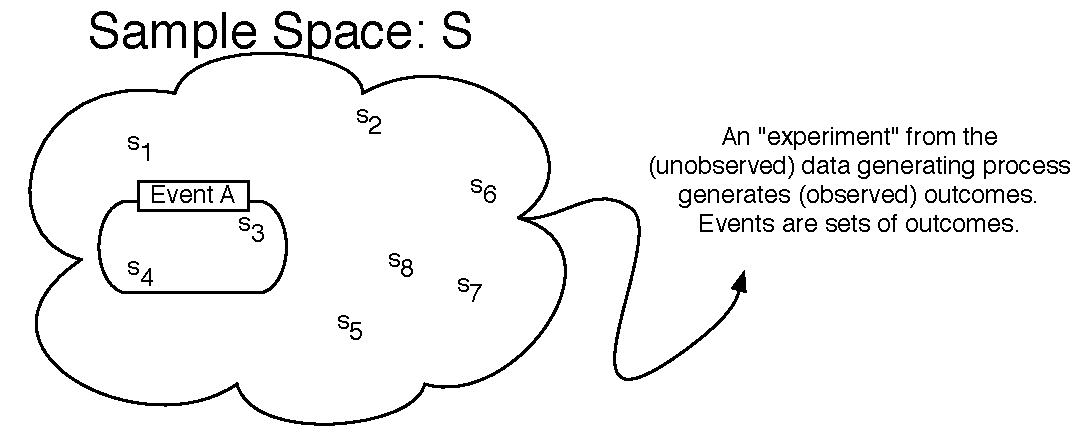
\includegraphics{./images/probability.pdf}

}

\caption{\label{fig-prob-image}Probablity as a Measure\footnote{Images
  of Probability and Random Variables drawn by Shiro Kuriwaki and
  inspired by Blitzstein and Morris}}

\end{figure}

\hypertarget{probability-definitions-formal-and-informal}{%
\subsection*{Probability Definitions: Formal and
Informal}\label{probability-definitions-formal-and-informal}}
\addcontentsline{toc}{subsection}{Probability Definitions: Formal and
Informal}

Many things in the world are uncertain. In everyday speech, we say that
we are \emph{uncertain} about the outcome of random events. Probability
is a formal model of uncertainty which provides a measure of uncertainty
governed by a particular set of rules (Figure~\ref{fig-prob-image}). A
different model of uncertainty would, of course, have a set of rules
different from anything we discuss here. Our focus on probability is
justified because it has proven to be a particularly useful model of
uncertainty.

\textbf{Probability Distribution Function}: a mapping of each event in
the sample space \(S\) to the real numbers that satisfy the following
three axioms (also called Kolmogorov's Axioms).

Formally,

\leavevmode\vadjust pre{\hypertarget{def-prob}{}}%
\begin{definition}[Probability]\label{def-prob}

Probability is a function that maps events to a real number, obeying the
axioms of probability.

\end{definition}

The axioms of probability make sure that the separate events add up in
terms of probability, and -- for standardization purposes -- that they
add up to 1.

\leavevmode\vadjust pre{\hypertarget{def-}{}}%
\begin{definition}[Axioms of Probability]\label{def-}

\begin{enumerate}
\def\labelenumi{\arabic{enumi}.}
\tightlist
\item
  For any event \(A\), \(P(A)\ge 0\).
\item
  \(P(S)=1\)
\item
  The Countable Additivity Axiom: For any sequence of \emph{disjoint}
  (mutually exclusive) events \(A_1,A_2,\ldots\) (of which there may be
  infinitely many), \[P\left( \bigcup\limits_{i=1}^k
  A_i\right)=\sum\limits_{i=1}^k P(A_i)\]
\end{enumerate}

The last axiom is an extension of a union to infinite sets. When there
are only two events in the space, it boils down to:

\begin{align*}
P(A_1 \cup A_2) = P(A_1) + P(A_2) \quad\text{for disjoint } A_1, A_2
\end{align*}

\end{definition}

\hypertarget{probability-operations}{%
\subsection*{Probability Operations}\label{probability-operations}}
\addcontentsline{toc}{subsection}{Probability Operations}

Using these three axioms, we can define all of the common rules of
probability.

\hypertarget{prop-prob}{}
\begin{enumerate}
\def\labelenumi{\arabic{enumi}.}
\tightlist
\item
  \(P(\emptyset)=0\)
\item
  For any event \(A\), \(0\le P(A) \le 1\)
\item
  \(P({A}^C)=1-P(A)\)
\item
  If \(A\subset B\) (\(A\) is a subset of \(B\)), then \(P(A)\le P(B)\)
\item
  For \emph{any} two events \(A\) and \(B\),
  \(P(A\cup B)=P(A)+P(B)-P(A\cap B)\)
\item
  Boole's Inequality: For any sequence of \(n\) events (which need not
  be disjoint) \(A_1,A_2,\ldots,A_n\), then
  \[P\left( \bigcup\limits_{i=1}^n A_i\right) \leq \sum\limits_{i=1}^n P(A_i)\]
\end{enumerate}

\leavevmode\vadjust pre{\hypertarget{exm-prob}{}}%
\begin{example}[]\label{exm-prob}

Assume we have an evenly-balanced, six-sided die.

Then,

\begin{enumerate}
\def\labelenumi{\arabic{enumi}.}
\tightlist
\item
  Sample space \(S\) =
\item
  \(P(1)=\cdots=P(6)=\)
\item
  \(P(\emptyset)=P(7)=\)
\item
  \(P\left( \{ 1, 3, 5 \} \right)=\)
\item
  \(P\left( \{ 1, 2 \}^C \right)= P\left( \{ 3, 4, 5, 6 \}\right)=\)
\item
  Let \(A=\{ 1,2,3,4,5 \}\subset S\). Then \(P(A)=5/6<P(S)=\)
\item
  Let \(A=\{ 1, 2, 3 \}\) and \(B=\{ 2, 4, 6 \}\). Then \(A\cup B\)?
  \(A\cap B\)? \(P(A \cup B)\)?
\end{enumerate}

\end{example}

\leavevmode\vadjust pre{\hypertarget{exr-prob1}{}}%
\begin{exercise}[]\label{exr-prob1}

Suppose you had a pair of four-sided dice. You sum the results from a
single toss. Let us call this sum, or the outcome, X.

\begin{enumerate}
\def\labelenumi{\arabic{enumi}.}
\tightlist
\item
  What is \(P(X = 5)\), \(P(X = 3)\), \(P(X = 6)\)?
\item
  What is \(P(X=5 \cup X = 3)^C\)?
\end{enumerate}

\end{exercise}

\hypertarget{conditional-probability}{%
\section{Conditional Probability}\label{conditional-probability}}

\textbf{Conditional Probability}: The conditional probability \(P(A|B)\)
of an event \(A\) is the probability of \(A\), given that another event
\(B\) has occurred. Conditional probability allows for the inclusion of
other information into the calculation of the probability of an event.
It is calculated as

\[P(A|B)=\frac{P(A\cap B)}{P(B)}\]

Note that conditional probabilities are probabilities and must also
follow the Kolmagorov axioms of probability.

\leavevmode\vadjust pre{\hypertarget{exm-condprobexm1}{}}%
\begin{example}[Conditional Probability]\label{exm-condprobexm1}

Assume \(A\) and \(B\) occur with the following frequencies: \(\quad\)

\begin{longtable}[]{@{}lcc@{}}
\toprule()
& \(A\) & \(A^c\) \\
\midrule()
\endhead
\(B\) & \(n_{ab}\) & \(n_{a^cb}\) \\
\(B^C\) & \(n_{ab^c}\) & \(n_{(ab)^c}\) \\
\bottomrule()
\end{longtable}

and let \(n_{ab}+n_{a^Cb}+n_{ab^C}+n_{(ab)^C}=N\). Then

\begin{enumerate}
\def\labelenumi{\arabic{enumi}.}
\tightlist
\item
  \(P(A)=\)
\item
  \(P(B)=\)
\item
  \(P(A\cap B)=\)
\item
  \(P(A|B)= \frac{P(A\cap B)}{P(B)}=\)
\item
  \(P(B|A)= \frac{P(A\cap B)}{P(A)}=\)
\end{enumerate}

\end{example}

\leavevmode\vadjust pre{\hypertarget{exm-condprobexm2}{}}%
\begin{example}[Conditional Probability 2]\label{exm-condprobexm2}

A six-sided die is rolled. What is the probability of a 1, given the
outcome is an odd number?

\end{example}

You could rearrange the fraction to highlight how a joint probability
could be expressed as the product of a conditional probability.

\leavevmode\vadjust pre{\hypertarget{def-}{}}%
\begin{definition}[Multiplicative Law of Probability]\label{def-}

The probability of the intersection of two events \(A\) and \(B\) is

\[P(A\cap B)=P(A)P(B|A)=P(B)P(A|B)\]

which follows directly from the definition of conditional probability.
More generally,

\begin{align*}
P(A_1\cap \cdots\cap A_k) = &P(A_k| A_{k-1}\cap \cdots \cap A_1) \\
\times &P(A_{k-1}|A_{k-2}\cap \cdots A_1) \\
\vdots & \\
\times &P(A_2|A_1) \\
\times &P(A_1)
\end{align*}

Sometimes it is easier to calculate these conditional probabilities and
sum them than it is to calculate \(P(A)\) directly.

\end{definition}

\leavevmode\vadjust pre{\hypertarget{def-}{}}%
\begin{definition}[Law of Total Probability]\label{def-}

Let \(S\) be the sample space of some experiment and let the disjoint
\(k\) events \(B_1,\ldots,B_k\) partition \(S\), such that
\(P(B_1\cup ... \cup B_k) = P(S) = 1\). If \(A\) is some other event in
\(S\), then the events \(A\cap B_1, A\cap B_2, \ldots, A\cap B_k\) will
form a partition of \(A\) and we can write \(A\) as
\[A=(A\cap B_1)\cup\cdots\cup (A\cap B_k)\].

Since the \(k\) events are disjoint,

\begin{align*}
P(A)&=\sum\limits_{i=1}^k P(A \cap B_i)\\
    &=\sum\limits_{i=1}^k P(B_i)P(A|B_i)
\end{align*}

\end{definition}

\hypertarget{bayes-rule}{%
\section{Bayes Rule}\label{bayes-rule}}

\textbf{Bayes Rule}: Assume that events \(B_1,\ldots,B_k\) form a
partition of the space \(S\). Then by the Law of Total Probability

\[P(B_j|A)= \frac{P(A \cap B_j)} {P(A)} = \frac{P(B_j) P(A|B_j)}{\sum\limits_{i=1}^k P(B_i)P(A|B_i)}\]

If there are only two states of \(B\), then this is just

\[P(B_1|A)=\frac{P(B_1)P(A|B_1)} {P(B_1)P(A|B_1)+P(B_2)P(A|B_2)}\]

Bayes' rule determines the posterior probability of a state \(P(B_j|A)\)
by calculating the probability \(P(A \cap B_j)\) that both the event
\(A\) and the state \(B_j\) will occur and dividing it by the
probability that the event will occur regardless of the state (by
summing across all \(B_i\)). The states could be something like
Normal/Defective, Healthy/Diseased, Republican/Democrat/Independent,
etc. The event on which one conditions could be something like a
sampling from a batch of components, a test for a disease, or a question
about a policy position.

\textbf{Prior and Posterior Probabilities}: Above, \(P(B_1)\) is often
called the prior probability, since it's the probability of \(B_1\)
before anything else is known. \(P(B_1|A)\) is called the posterior
probability, since it's the probability after other information is taken
into account.

\leavevmode\vadjust pre{\hypertarget{exm-bayesrule}{}}%
\begin{example}[Bayes' Rule]\label{exm-bayesrule}

In a given town, 40\% of the voters are Democrat and 60\% are
Republican. The president's budget is supported by 50\% of the Democrats
and 90\% of the Republicans. If a randomly (equally likely) selected
voter is found to support the president's budget, what is the
probability that they are a Democrat?

\end{example}

\leavevmode\vadjust pre{\hypertarget{exr-condprobexr}{}}%
\begin{exercise}[Conditional Probability]\label{exr-condprobexr}

Assume that 2\% of the population of the U.S. are members of some
extremist militia group. We develop a survey that positively classifies
someone as being a member of a militia group given that they are a
member 95\% of the time and negatively classifies someone as not being a
member of a militia group given that they are not a member 97\% of the
time. What is the probability that someone positively classified as
being a member of a militia group is actually a militia member?

\end{exercise}

\hypertarget{independence}{%
\section{Independence}\label{independence}}

\leavevmode\vadjust pre{\hypertarget{def-}{}}%
\begin{definition}[Independence]\label{def-}

If the occurrence or nonoccurrence of either events \(A\) and \(B\) have
no effect on the occurrence or nonoccurrence of the other, then \(A\)
and \(B\) are independent.

\end{definition}

If \(A\) and \(B\) are independent, then

\hypertarget{prop-}{}
\begin{enumerate}
\def\labelenumi{\arabic{enumi}.}
\tightlist
\item
  \(P(A|B)=P(A)\)
\item
  \(P(B|A)=P(B)\)
\item
  \(P(A\cap B)=P(A)P(B)\)
\item
  More generally than the above,
  \(P(\bigcap_{i=1}^k A_i) = \prod_{i = 1}^K P(A_i)\)
\end{enumerate}

Are mutually exclusive events independent of each other?

No.~If A and B are mutually exclusive, then they cannot happen
simultaneously. If we know that A occurred, then we know that B couldn't
have occurred. Because of this, A and B aren't independent.

\textbf{Pairwise Independence}: A set of more than two events
\(A_1, A_2, \dots, A_k\) is pairwise independent if
\(P(A_i\cap A_j)=P(A_i)P(A_j)\), \(\forall i\neq j\). Note that this
does \textbf{not} necessarily imply joint independence.

\textbf{Conditional Independence}: If \(A\) and \(B\) are independent
once you know the occurrence of a third event \(C\), then \(A\) and
\(B\) are conditionally independent (conditional on \(C\)):

\begin{enumerate}
\def\labelenumi{\arabic{enumi}.}
\tightlist
\item
  \(P(A|B \cap C)=P(A|C)\)
\item
  \(P(B|A \cap C)=P(B|C)\)
\item
  \(P(A\cap B|C)=P(A|C)P(B|C)\)
\end{enumerate}

Just because two events are conditionally independent does not mean that
they are independent. Actually it is hard to think of real-world things
that are ``unconditionally'' independent. That's why it's always
important to ask about a finding: What was it conditioned on? For
example, suppose that a graduate school admission decisions are done by
only one professor, who picks a group of 50 bright students and flips a
coin for each student to generate a class of about 25 students. Then the
the probability that two students get accepted are conditionally
independent, because they are determined by two separate coin tosses.
However, this does not mean that their admittance is not completely
independent. Knowing that student \(A\) got in gives us information
about whether student \(B\) got in, if we think that the professor
originally picked her pool of 50 students by merit.

Perhaps more counter-intuitively: If two events are already independent,
then it might seem that no amount of ``conditioning'' will make them
dependent. But this is not always so. For example\footnote{Example taken
  from Blitzstein and Hwang, Example 2.5.10}, suppose I only get a call
from two people, Alice and Bob. Let \(A\) be the event that Alice calls,
and \(B\) be the event that Bob calls. Alice and Bob do not communicate,
so \(P(A \mid B) = P(A).\) But now let \(C\) be the event that your
phone rings. For conditional independence to hold here, then
\(P(A \mid C)\) must be equal to \(P(A \mid B \cap C).\) But this is not
true -- \(A \mid C\) may or may not be true, but \(P(A \mid B \cap C)\)
certainly is true.

\hypertarget{random-variables}{%
\section{Random Variables}\label{random-variables}}

Most questions in the social sciences involve events, rather than
numbers per se. To analyze and reason about events quantitatively, we
need a way of mapping events to numbers. A random variable does exactly
that.

\begin{figure}

{\centering 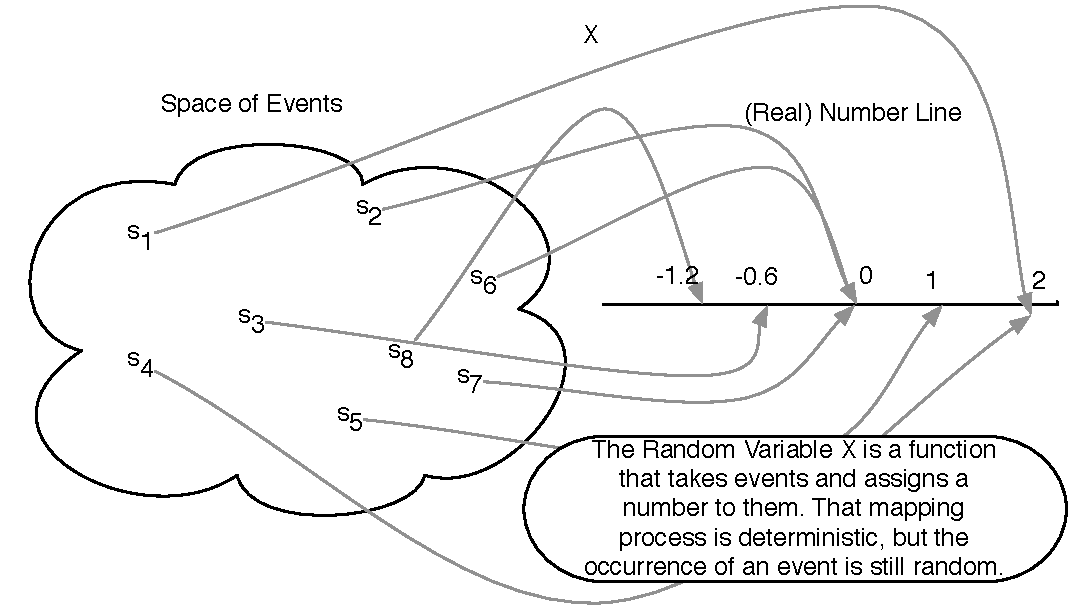
\includegraphics{./images/rv.pdf}

}

\caption{\label{fig-rv-image}The Random Variable as a Real-Valued
Function}

\end{figure}

\leavevmode\vadjust pre{\hypertarget{def-}{}}%
\begin{definition}[Random Variable]\label{def-}

A random variable is a measurable function \(X\) that maps from the
sample space \(S\) to the set of real numbers \(R.\) It assigns a real
number to every outcome \(s \in S\).

\end{definition}

Figure~\ref{fig-rv-image} shows a image of the function. It might seem
strange to define a random variable as a function -- which is neither
random nor variable. The randomness comes from the realization of an
event from the sample space \(s\).

\textbf{Randomness} means that the outcome of some experiment is not
deterministic, i.e.~there is some probability (\(0 < P(A) < 1\)) that
the event will occur.

The support of a random variable is all values for which there is a
positive probability of occurrence.

Example: Flip a fair coin two times. What is the sample space?

A random variable must map events to the real line. For example, let a
random variable \(X\) be the number of heads. The event \((H, H)\) gets
mapped to 2 \(X(s) = 2\), and the events \(\{(H, T), (T, H)\}\) gets
mapped to 1 \((X(s) = 1)\), the event \((T, T)\) gets mapped to 0
\((X(s) = 0)\).

What are other possible random variables?

\hypertarget{distributions}{%
\section{Distributions}\label{distributions}}

We now have two main concepts in this section -- probability and random
variables. Given a sample space \(S\) and the same experiment, both
probability and random variables take events as their inputs. But they
output different things (probabilities measure the ``size'' of events,
random variables give a number in a way that the analyst chose to define
the random variable). How do the two concepts relate?

The concept of distributions is the natural bridge between these two
concepts.

\leavevmode\vadjust pre{\hypertarget{def-}{}}%
\begin{definition}[Distribution of a random variable]\label{def-}

A distribution of a random variable is a function that specifies the
probabilities of all events associated with that random variable. There
are several types of distributions: A probability mass function for a
discrete random variable and probability density function for a
continuous random variable.

\end{definition}

Notice how the definition of distributions combines two ideas of random
variables and probabilities of events. First, the distribution considers
a random variable, call it \(X\). \(X\) can take a number of possible
numeric values.

\leavevmode\vadjust pre{\hypertarget{exm-}{}}%
\begin{example}[]\label{exm-}

Consider three binary outcomes, one for each patient recovering from a
disease: \(R_i\) denotes the event in which patient \(i\)
(\(i = 1, 2, 3\)) recovers from a disease. \(R_1\), \(R_2\), and
\(R_3\). How would we represent the total number of people who end up
recovering from the disease?

\end{example}

\begin{solution}

Define the random variable \(X\) be the total number of people (out of
three) who recover from the disease. Random variables are functions,
that take as an input a set of events (in the sample space \(S\)) and
deterministically assigns them to a number of the analyst's choice.

Recall that with each of these numerical values there is a class of
\emph{events}. In the previous example,

\begin{itemize}
\tightlist
\item
  For \(X = 3\) there is one outcome (\(R_1, R_2, R_3\))
\item
  For \(X = 1\) there are multiple
  \(\{(R_1, R_2^c, R_3^c), (R_1^c, R_2, R_3^c), (R_1^c, R_2^c, R_3), \}\)
\end{itemize}

Now, the thing to notice here is that each of these events naturally
come with a probability associated with them. That is,
\(P(R_1, R_2, R_3)\) is a number from 0 to 1, as is
\(P(R_1, R_2^c, R_3^c)\). These all have probabilities because they are
in the sample space \(S\). The function that tells us these
probabilities that are associated with a numerical value of a random
variable is called a distribution.

In other words, a random variable \(X\) \emph{induces a probability
distribution} \(P\) (sometimes written \(P_X\) to emphasize that the
probability density is about the r.v. \(X\))

\end{solution}

\hypertarget{discrete-random-variables}{%
\subsection*{Discrete Random
Variables}\label{discrete-random-variables}}
\addcontentsline{toc}{subsection}{Discrete Random Variables}

The formal definition of a random variable is easier to given by
separating out two cases: discrete random variables when the numeric
summaries of the events are discrete, and continuous random variables
when they are continuous.

\leavevmode\vadjust pre{\hypertarget{def-}{}}%
\begin{definition}[Discrete Random Variable]\label{def-}

\(X\) is a discrete random variable if it can assume only a finite or
countably infinite number of distinct values. Examples: number of wars
per year, heads or tails.

\end{definition}

The distribution of a discrete r.v. is a PMF:

\leavevmode\vadjust pre{\hypertarget{def-}{}}%
\begin{definition}[Probability Mass Function]\label{def-}

For a discrete random variable \(X\), the probability mass function
(Also referred to simply as the ``probability distribution.'') (PMF),
\(p(x)=P(X=x)\), assigns probabilities to a countable number of distinct
\(x\) values such that

\begin{enumerate}
\def\labelenumi{\arabic{enumi}.}
\tightlist
\item
  \(0\le p(x)\le 1\)
\item
  \(\sum\limits_y p(x)=1\)
\end{enumerate}

\end{definition}

\leavevmode\vadjust pre{\hypertarget{exm-}{}}%
\begin{example}[]\label{exm-}

For a fair six-sided die, there is an equal probability of rolling any
number. Since there are six sides, the probability mass function is then
\(p(y)=1/6\) for \(y=1,\ldots,6\), 0 otherwise.

\end{example}

In a discrete random variable, \textbf{cumulative distribution function}
(Also referred to simply as the ``cumulative distribution'' or
previously as the ``distribution function''), \(F(x)\) or \(P(X\le x)\),
is the probability that \(X\) is less than or equal to some value \(x\),
or \[P(X\le x)=\sum\limits_{i\le x} p(i)\]

Properties a CDF must satisfy:

\begin{enumerate}
\def\labelenumi{\arabic{enumi}.}
\tightlist
\item
  \(F(x)\) is non-decreasing in \(x\).
\item
  \(\lim\limits_{x \to -\infty} F(x) = 0\) and
  \(\lim\limits_{x \to \infty} F(x) = 1\)
\item
  \(F(x)\) is right-continuous.
\end{enumerate}

Note that \(P(X > x) = 1 - P(X \le x)\).

\leavevmode\vadjust pre{\hypertarget{exm-}{}}%
\begin{example}[]\label{exm-}

For a fair die with its value as \(Y\), What are the following?

\begin{enumerate}
\def\labelenumi{\arabic{enumi}.}
\tightlist
\item
  \(P(Y\le 1)\)
\item
  \(P(Y\le 3)\)
\item
  \(P(Y\le 6)\)
\end{enumerate}

\end{example}

\hypertarget{continuous-random-variables}{%
\subsection*{Continuous Random
Variables}\label{continuous-random-variables}}
\addcontentsline{toc}{subsection}{Continuous Random Variables}

We also have a similar definition for \emph{continuous} random
variables.

\leavevmode\vadjust pre{\hypertarget{def-}{}}%
\begin{definition}[Continuous Random Variable]\label{def-}

\(X\) is a continuous random variable if there exists a nonnegative
function \(f(x)\) defined for all real \(x\in (-\infty,\infty)\), such
that for any interval \(A\), \(P(X\in A)=\int\limits_A f(x)dx\).
Examples: age, income, GNP, temperature.

\end{definition}

\leavevmode\vadjust pre{\hypertarget{def-}{}}%
\begin{definition}[Probability Density Function]\label{def-}

The function \(f\) above is called the probability density function
(pdf) of \(X\) and must satisfy

\[f(x)\ge 0\]

\[\int\limits_{-\infty}^\infty f(x)dx=1\]

Note also that \(P(X = x)=0\) --- i.e., the probability of any point
\(y\) is zero.

\end{definition}

For both discrete and continuous random variables, we have a unifying
concept of another measure: the cumulative distribution:

\leavevmode\vadjust pre{\hypertarget{def-}{}}%
\begin{definition}[Cumulative Distribution Function]\label{def-}

Because the probability that a continuous random variable will assume
any particular value is zero, we can only make statements about the
probability of a continuous random variable being within an interval.
The cumulative distribution gives the probability that \(Y\) lies on the
interval \((-\infty,y)\) and is defined as
\[F(x)=P(X\le x)=\int\limits_{-\infty}^x f(s)ds.\] Note that \(F(x)\)
has similar properties with continuous distributions as it does with
discrete - non-decreasing, continuous (not just right-continuous), and
\(\lim\limits_{x \to -\infty} F(x) = 0\) and
\(\lim\limits_{x \to \infty} F(x) = 1\).

\end{definition}

We can also make statements about the probability of \(Y\) falling in an
interval \(a\le y\le b\).

\[P(a\le x\le b)=\int\limits_a^b f(x)dx\]

The PDF and CDF are linked by the integral: The CDF of the integral of
the PDF: \[f(x) = F'(x)=\frac{dF(x)}{dx}\]

\leavevmode\vadjust pre{\hypertarget{exm-}{}}%
\begin{example}[]\label{exm-}

For \(f(y)=1, \quad 0<y<1\), find: (1) The CDF \(F(y)\) and (2) The
probability \(P(0.5<y<0.75)\).

\end{example}

\hypertarget{answers-to-examples-and-exercises-3}{%
\section*{Answers to Examples and
Exercises}\label{answers-to-examples-and-exercises-3}}
\addcontentsline{toc}{section}{Answers to Examples and Exercises}

Answer to Example~\ref{exm-counting}:

\begin{enumerate}
\def\labelenumi{\arabic{enumi}.}
\item
  \(5 \times 5 \times 5 = 125\)
\item
  \(5 \times 4 \times 3 = 60\)
\item
  \(\binom{5}{3} = \frac{5!}{(5-3)!3!} = \frac{5 \times 4}{2 \times 1} = 10\)
\end{enumerate}

Answer to Exercise~\ref{exr-counting1}:

\begin{enumerate}
\def\labelenumi{\arabic{enumi}.}
\tightlist
\item
  \(\binom{52}{4} = \frac{52!}{(52-4)!4!} = 270725\)
\end{enumerate}

Answer to Example~\ref{exm-sets}:

\begin{enumerate}
\def\labelenumi{\arabic{enumi}.}
\tightlist
\item
  \{1, 2, 3, 4, 5, 6\}
\item
  \{5, 6\}
\item
  \{1, 2, 7, 8, 9, 10\}
\item
  \{3, 4\}
\end{enumerate}

Answer to Exercise~\ref{exr-sets1}:

Sample Space: \{2, 3, 4, 5, 6, 7, 8\}

\begin{enumerate}
\def\labelenumi{\arabic{enumi}.}
\tightlist
\item
  \{3, 4, 5, 6, 7\}
\item
  \{4, 5, 6\}
\end{enumerate}

Answer to Example~\ref{exm-prob}:

\begin{enumerate}
\def\labelenumi{\arabic{enumi}.}
\item
  \({1, 2, 3, 4, 5, 6}\)
\item
  \(\frac{1}{6}\)
\item
  \(0\)
\item
  \(\frac{1}{2}\)
\item
  \(\frac{4}{6} = \frac{2}{3}\)
\item
  \(1\)
\item
  \(A\cup B=\{1, 2, 3, 4, 6\}\), \(A\cap B=\{2\}\), \(\frac{5}{6}\)
\end{enumerate}

Answer to Exercise~\ref{exr-prob1}:

\begin{enumerate}
\def\labelenumi{\arabic{enumi}.}
\item
  \(P(X = 5) = \frac{4}{16}\), \(P(X = 3) = \frac{2}{16}\),
  \(P(X = 6) = \frac{3}{16}\)
\item
  What is \(P(X=5 \cup X = 3)^C = \frac{10}{16}\)?
\end{enumerate}

Answer to Example~\ref{exm-condprobexm1}:

\begin{enumerate}
\def\labelenumi{\arabic{enumi}.}
\item
  \(\frac{n_{ab} + n_{ab^c}}{N}\)
\item
  \(\frac{n_{ab} + n_{a^cb}}{N}\)
\item
  \(\frac{n_{ab}}{N}\)
\item
  \(\frac{\frac{n_{ab}}{N}}{\frac{n_{ab} + n_{a^cb}}{N}} = \frac{n_{ab}}{n_{ab} + n_{a^cb}}\)
\item
  \(\frac{\frac{n_{ab}}{N}}{\frac{n_{ab} + n_{ab^c}}{N}} = \frac{n_{ab}}{n_{ab} + n_{ab^c}}\)
\end{enumerate}

Answer to Example~\ref{exm-condprobexm2}:

\(P(1|Odd) = \frac{P(1 \cap Odd)}{P(Odd)} = \frac{\frac{1}{6}}{\frac{1}{2}} = \frac{1}{3}\)

Answer to Example~\ref{exm-bayesrule}:

We are given that

\[P(D) = .4, P(D^c) = .6, P(S|D) = .5, P(S|D^c) = .9\]

Using this, Bayes' Law and the Law of Total Probability, we know:

\[P(D|S) = \frac{P(D)P(S|D)}{P(D)P(S|D) + P(D^c)P(S|D^c)}\]

\[P(D|S) = \frac{.4 \times .5}{.4 \times .5 + .6 \times .9 } = .27\]

Answer to Exercise~\ref{exr-condprobexr}:

We are given that

\[P(M) = .02, P(C|M) = .95, P(C^c|M^c) = .97\]

\[P(M|C) = \frac{P(C|M)P(M)}{P(C)}\]

\[= \frac{P(C|M)P(M)}{P(C|M)P(M) + P(C|M^c)P(M^c)}\]

\[= \frac{P(C|M)P(M)}{P(C|M)P(M) + [1-P(C^c|M^c)]P(M^c)}\]

\[ = \frac{.95 \times .02}{.95 \times .02 + .03 \times .98} = .38\]

\hypertarget{distribution}{%
\chapter{Summarizing Distributions}\label{distribution}}

\hypertarget{expectation}{%
\section{Expectation}\label{expectation}}

We often want to summarize some characteristics of the distribution of a
random variable. The most important summary is the expectation (or
expected value, or mean), in which the possible values of a random
variable are weighted by their probabilities.

\leavevmode\vadjust pre{\hypertarget{def-}{}}%
\begin{definition}[Expectation of a Discrete Random
Variable]\label{def-}

The expected value of a discrete random variable \(Y\) is

\[E(Y)=\sum\limits_{y} y P(Y=y)= \sum\limits_{y} y p(y)\]

In words, it is the weighted average of all possible values of \(Y\),
weighted by the probability that \(y\) occurs. It is not necessarily the
number we would expect \(Y\) to take on, but the average value of \(Y\)
after a large number of repetitions of an experiment.

\end{definition}

\leavevmode\vadjust pre{\hypertarget{exm-expectdiscrete}{}}%
\begin{example}[]\label{exm-expectdiscrete}

What is the expectation of a fair, six-sided die?

\end{example}

\textbf{Expectation of a Continuous Random Variable}: The expected value
of a continuous random variable is similar in concept to that of the
discrete random variable, except that instead of summing using
probabilities as weights, we integrate using the density to weight.
Hence, the expected value of the continuous variable \(Y\) is defined by

\[E(Y)=\int\limits_{y} y f(y) dy\]

\leavevmode\vadjust pre{\hypertarget{exm-expectconti}{}}%
\begin{example}[Expectation of a Continuous Random
Variable]\label{exm-expectconti}

Find \(E(Y)\) for \(f(y)=\frac{1}{1.5}, \quad 0<y<1.5\).

\end{example}

\hypertarget{expected-value-of-a-function}{%
\subsection*{Expected Value of a
Function}\label{expected-value-of-a-function}}
\addcontentsline{toc}{subsection}{Expected Value of a Function}

Remember: An Expected Value is a type of weighted average. We can extend
this to composite functions. For random variable \(Y\),

If \(Y\) is Discrete with PMF \(p(y)\),

\[E[g(Y)]=\sum\limits_y g(y)p(y)\]

If \(Y\) is Continuous with PDF \(f(y)\),

\[E[g(Y)]=\int\limits_{-\infty}^\infty g(y)f(y)dy\]

\hypertarget{properties-of-expected-values}{%
\subsection*{Properties of Expected
Values}\label{properties-of-expected-values}}
\addcontentsline{toc}{subsection}{Properties of Expected Values}

Dealing with Expectations is easier when the thing inside is a sum. The
intuition behind this that Expectation is an integral, which is a type
of sum.

\hypertarget{prop-}{}
\begin{enumerate}
\def\labelenumi{\arabic{enumi}.}
\tightlist
\item
  Expectation of a constant is a constant \[E(c)=c\]
\item
  Constants come out \[E(c g(Y))= c E(g(Y))\]
\item
  Expectation is Linear
  \[E(g(Y_1) + \cdots + g(Y_n))=E(g(Y_1)) +\cdots+E(g(Y_n)),\]
  regardless of independence
\item
  Expected Value of Expected Values: \[E(E(Y)) = E(Y)\] (because the
  expected value of a random variable is a constant)
\end{enumerate}

Finally, if \(X\) and \(Y\) are independent, even products are easy:

\[X \;\; \mathrm{ and } \;\; Y \mathrm{are independent } \;\Rightarrow\; E(XY) = E(X)E(Y)\]

\textbf{Conditional Expectation}: With joint distributions, we are often
interested in the expected value of a variable \(Y\) if we could hold
the other variable \(X\) fixed. This is the conditional expectation of
\(Y\) given \(X = x\):

\begin{enumerate}
\def\labelenumi{\arabic{enumi}.}
\tightlist
\item
  \(Y\) discrete: \(E(Y|X = x) = \sum_y yp_{Y|X}(y|x)\)
\item
  \(Y\) continuous: \(E(Y|X = x) = \int_y yf_{Y|X}(y|x)dy\)
\end{enumerate}

The conditional expectation is often used for prediction when one knows
the value of \(X\) but not \(Y\)

\hypertarget{variance-and-covariance}{%
\section{Variance and Covariance}\label{variance-and-covariance}}

We can also look at other summaries of the distribution, which build on
the idea of taking expectations. Variance tells us about the ``spread''
of the distribution; it is the expected value of the squared deviations
from the mean of the distribution. The standard deviation is simply the
square root of the variance.

\leavevmode\vadjust pre{\hypertarget{def-}{}}%
\begin{definition}[Variance]\label{def-}

The Variance of a Random Variable \(Y\) is

\[\text{Var}(Y) = E[(Y - E(Y))^2] =  E(Y^2)-[E(Y)]^2\]

The Standard Deviation is the square root of the variance :

\[SD(Y) = \sigma_Y= \sqrt{\text{Var}(Y)}\]

\end{definition}

\leavevmode\vadjust pre{\hypertarget{exm-var}{}}%
\begin{example}[]\label{exm-var}

Given the following PMF:

\[f(x) = \begin{cases}
    \frac{3!}{x!(3-x)!}(\frac{1}{2})^3 \quad x = 0,1,2,3\\
      0 \quad otherwise
  \end{cases}\]

What is \(\text{Var}(x)\)?

\textbf{Hint:} First calculate \(E(X)\) and \(E(X^2)\)

\end{example}

\leavevmode\vadjust pre{\hypertarget{def-}{}}%
\begin{definition}[Covariance]\label{def-}

The covariance measures the degree to which two random variables vary
together; if the covariance between \(X\) and \(Y\) is positive, X tends
to be larger than its mean when Y is larger than its mean.

\[\text{Cov}(X,Y) = E[(X - E(X))(Y - E(Y))] \]

We can also write this as

\begin{align*}
\text{Cov}(X,Y) &= E\left(XY - XE(Y) - E(X)Y + E(X)E(Y)\right)\\
&= E(XY) - E(X)E(Y) - E(X)E(Y) + E(X)E(Y)\\
&= E(XY) - E(X)E(Y)
\end{align*}

\end{definition}

The covariance of a variable with itself is the variance of that
variable.

The Covariance is unfortunately hard to interpret in magnitude. The
correlation is a standardized version of the covariance, and always
ranges from -1 to 1.

\leavevmode\vadjust pre{\hypertarget{def-}{}}%
\begin{definition}[Correlation]\label{def-}

The correlation coefficient is the covariance divided by the standard
deviations of \(X\) and \(Y\). It is a unitless measure and always takes
on values in the interval \([-1,1]\).

\[\text{Corr}(X, Y) = \frac{\text{Cov}(X,Y)}{\sqrt{\text{Var}(X)\text{Var}(Y)}} = \frac{\text{Cov}(X,Y)}{SD(X)SD(Y)}\]

\end{definition}

\textbf{\emph{Properties of Variance and Covariance:}}

\hypertarget{prop-}{}
\begin{enumerate}
\def\labelenumi{\arabic{enumi}.}
\tightlist
\item
  \(\text{Var}(c) = 0\)
\item
  \(\text{Var}(cY) = c^2 \text{Var}(Y)\)
\item
  \(\text{Cov}(Y,Y) = \text{Var}(Y)\)
\item
  \(\text{Cov}(X,Y) = \text{Cov}(Y,X)\)
\item
  \(\text{Cov}(aX,bY) = ab \text{Cov}(X,Y)\)
\item
  \(\text{Cov}(X+a,Y) = \text{Cov}(X,Y)\)
\item
  \(\text{Cov}(X+Z,Y+W) = \text{Cov}(X,Y) + \text{Cov}(X,W) + \text{Cov}(Z,Y) + \text{Cov}(Z,W)\)
\item
  \(\text{Var}(X+Y) = \text{Var}(X) + \text{Var}(Y) + 2\text{Cov}(X,Y)\)
\end{enumerate}

\leavevmode\vadjust pre{\hypertarget{exr-expvar}{}}%
\begin{exercise}[Expectation and Variance]\label{exr-expvar}

Suppose we have a PMF with the following characteristics: \begin{align*}
  P(X = -2) &= \frac{1}{5}\\
  P(X = -1) &= \frac{1}{6}\\
  P(X = 0) &= \frac{1}{5}\\
  P(X = 1) &= \frac{1}{15}\\
  P(X = 2) &= \frac{11}{30}
\end{align*}

\begin{enumerate}
\def\labelenumi{\arabic{enumi}.}
\tightlist
\item
  Calculate the expected value of X
\end{enumerate}

Define the random variable \(Y = X^2\).

\begin{enumerate}
\def\labelenumi{\arabic{enumi}.}
\setcounter{enumi}{1}
\item
  Calculate the expected value of \(Y\). (Hint: It would help to derive
  the PMF of \(Y\) first in order to calculate the expected value of
  \(Y\) in a straightforward way)
\item
  Calculate the variance of \(X\).
\end{enumerate}

\end{exercise}

\leavevmode\vadjust pre{\hypertarget{exr-expvar2}{}}%
\begin{exercise}[]\label{exr-expvar2}

Given the following PDF:

\[f(x) = \begin{cases} \frac{3}{10}(3x - x^2) \quad 0 \leq x \leq 2\\ 0 \quad \mathrm{ otherwise} \end{cases}\]

Find the expectation and variance of \(X\).

\end{exercise}

\leavevmode\vadjust pre{\hypertarget{exr-expvar3}{}}%
\begin{exercise}[]\label{exr-expvar3}

Find the mean and standard deviation of random variable \(X\). The PDF
of this \(X\) is as follows:

\[f(x) = \begin{cases} \frac{1}{4}x \quad 0 \leq x \leq 2\\ \frac{1}{4}(4 - x)  \quad 2 \leq x \leq 4\\ 0 \quad \mathrm{ otherwise} \end{cases}\]

Next, calculate \(P(X < \mu - \sigma)\) Remember, \(\mu\) is the mean
and \(\sigma\) is the standard deviation.

\end{exercise}

\hypertarget{common-distributions}{%
\section{Common Distributions}\label{common-distributions}}

Two \emph{discrete} distributions used often are:

\leavevmode\vadjust pre{\hypertarget{def-}{}}%
\begin{definition}[Binomial Distribution]\label{def-}

\(Y\) is distributed binomial if it represents the number of
``successes'' observed in \(n\) independent, identical ``trials,'' where
the probability of success in any trial is \(p\) and the probability of
failure is \(q=1-p\).

\end{definition}

For any particular sequence of \(y\) successes and \(n-y\) failures, the
probability of obtaining that sequence is \(p^y q^{n-y}\) (by the
multiplicative law and independence). However, there are
\(\binom{n}{y}=\frac{n!}{(n-y)!y!}\) ways of obtaining a sequence with
\(y\) successes and \(n-y\) failures. So the binomial distribution is
given by \[p(y)=\binom{n}{y}p^y q^{n-y}, \quad y=0,1,2,\ldots,n\] with
mean \(\mu=E(Y)=np\) and variance \(\sigma^2=\text{Var}(Y)=npq\).

\leavevmode\vadjust pre{\hypertarget{exm-}{}}%
\begin{example}[]\label{exm-}

Republicans vote for Democrat-sponsored bills 2\% of the time. What is
the probability that out of 10 Republicans questioned, half voted for a
particular Democrat-sponsored bill? What is the mean number of
Republicans voting for Democrat-sponsored bills? The variance? 1.
\(P(Y=5)=\) 2. \(E(Y)=\) 3. \(\text{Var}(Y)=6\)

\end{example}

\leavevmode\vadjust pre{\hypertarget{def-}{}}%
\begin{definition}[Poisson Distribution]\label{def-}

A random variable \(Y\) has a Poisson distribution if

\[P(Y = y)=\frac{\lambda^y}{y!}e^{-\lambda}, \quad y=0,1,2,\ldots, \quad \lambda>0\]

The Poisson has the unusual feature that its expectation equals its
variance: \(E(Y)=\text{Var}(Y)=\lambda\). The Poisson distribution is
often used to model rare event counts: counts of the number of events
that occur during some unit of time. \(\lambda\) is often called the
``arrival rate.''

\end{definition}

\leavevmode\vadjust pre{\hypertarget{exm-}{}}%
\begin{example}[]\label{exm-}

Border disputes occur between two countries through a Poisson
Distribution, at a rate of 2 per month. What is the probability of 0, 2,
and less than 5 disputes occurring in a month?

\end{example}

Two \emph{continuous} distributions used often are:

\leavevmode\vadjust pre{\hypertarget{def-}{}}%
\begin{definition}[Uniform Distribution]\label{def-}

A random variable \(Y\) has a continuous uniform distribution on the
interval \((\alpha,\beta)\) if its density is given by
\[f(y)=\frac{1}{\beta-\alpha}, \quad \alpha\le y\le \beta\] The mean and
variance of \(Y\) are \(E(Y)=\frac{\alpha+\beta}{2}\) and
\(\text{Var}(Y)=\frac{(\beta-\alpha)^2}{12}\).

\end{definition}

\leavevmode\vadjust pre{\hypertarget{exm-}{}}%
\begin{example}[]\label{exm-}

For \(Y\) uniformly distributed over \((1,3)\), what are the following
probabilities?

\begin{enumerate}
\def\labelenumi{\arabic{enumi}.}
\tightlist
\item
  \(P(Y=2)\)
\item
  Its density evaluated at 2, or \(f(2)\)
\item
  \(P(Y \le 2)\)
\item
  \(P(Y > 2)\)
\end{enumerate}

\end{example}

\leavevmode\vadjust pre{\hypertarget{def-}{}}%
\begin{definition}[Normal Distribution]\label{def-}

A random variable \(Y\) is normally distributed with mean \(E(Y)=\mu\)
and variance \(\text{Var}(Y)=\sigma^2\) if its density is

\[f(y)=\frac{1}{\sqrt{2\pi}\sigma}e^{-\frac{(y-\mu)^2}{2\sigma^2}}\]

\end{definition}

See Figure Figure~\ref{fig-normaldens} are various Normal Distributions
with the same \(\mu = 1\) and two versions of the variance.

\begin{figure}

{\centering 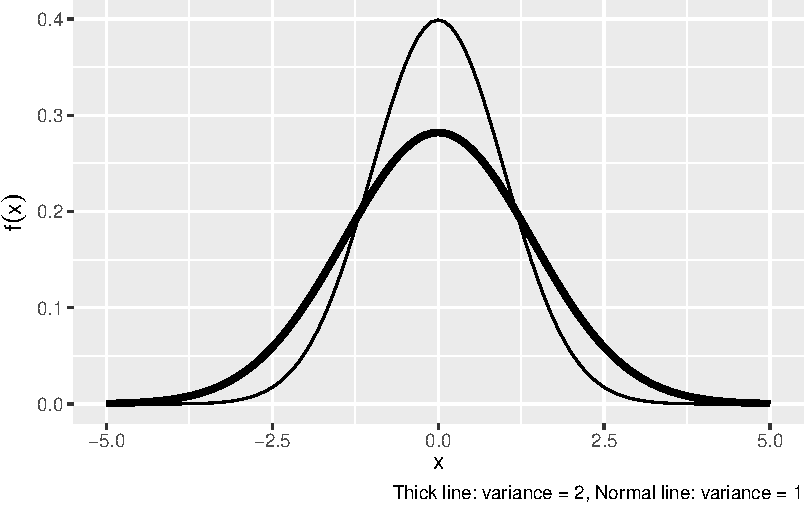
\includegraphics{./42_distribution_files/figure-pdf/fig-normaldens-1.pdf}

}

\caption{\label{fig-normaldens}Normal Distribution Density}

\end{figure}

\hypertarget{joint-distributions}{%
\section{Joint Distributions}\label{joint-distributions}}

Often, we are interested in two or more random variables defined on the
same sample space. The distribution of these variables is called a joint
distribution. Joint distributions can be made up of any combination of
discrete and continuous random variables.

\textbf{Joint Probability Distribution}: If both \(X\) and \(Y\) are
random variable, their joint probability mass/density function assigns
probabilities to each pair of outcomes

Discrete:

\[p(x, y) = P(X = x, Y = y)\]

such that \(p(x,y) \in [0,1]\) and \[\sum\sum p(x,y) = 1\]

Continuous:

\[f(x,y);P((X,Y) \in A) = \int\!\!\!\int_A f(x,y)dx dy \]

s.t. \(f(x,y)\ge 0\) and

\[\int_{-\infty}^\infty\int_{-\infty}^\infty f(x,y)dxdy = 1\]

If X and Y are independent, then \(P(X=x,Y=y) = P(X=x)P(Y=y)\) and
\(f(x,y) = f(x)f(y)\)

\textbf{Marginal Probability Distribution}: probability distribution of
only one of the two variables (ignoring information about the other
variable), we can obtain the marginal distribution by
summing/integrating across the variable that we don't care about:

\begin{itemize}
\tightlist
\item
  Discrete: \(p_X(x) = \sum_i p(x, y_i)\)
\item
  Continuous: \(f_X(x) = \int_{-\infty}^\infty f(x,y)dy\)
\end{itemize}

\textbf{Conditional Probability Distribution}: probability distribution
for one variable, holding the other variable fixed. Recalling from the
previous lecture that \(P(A|B)=\frac{P(A\cap B)}{P(B)}\), we can write
the conditional distribution as

\begin{itemize}
\tightlist
\item
  Discrete: \(p_{Y|X}(y|x) = \frac{p(x,y)}{p_X(x)}, \quad p_X(x) > 0\)
\item
  Continuous: \(f_{Y|X}(y|x) = \frac{f(x,y)}{f_X(x)},\quad f_X(x) > 0\)
\end{itemize}

\leavevmode\vadjust pre{\hypertarget{exr-}{}}%
\begin{exercise}[]\label{exr-}

Suppose we are interested in the outcomes of flipping a coin and rolling
a 6-sided die at the same time. The sample space for this process
contains 12 elements:
\[\{(H, 1), (H, 2), (H, 3), (H, 4), (H, 5), (H, 6), (T, 1), (T, 2), (T, 3), (T, 4), (T, 5), (T, 6)\}\]
We can define two random variables \(X\) and \(Y\) such that \(X = 1\)
if heads and \(X = 0\) if tails, while \(Y\) equals the number on the
die.

We can then make statements about the joint distribution of \(X\) and
\(Y\). What are the following?

\begin{enumerate}
\def\labelenumi{\arabic{enumi}.}
\tightlist
\item
  \(P(X=x)\)
\item
  \(P(Y=y)\)
\item
  \(P(X=x, Y=y)\)
\item
  \(P(X=x|Y=y)\)
\item
  Are X and Y independent?
\end{enumerate}

\end{exercise}

\hypertarget{answers-to-examples-and-exercises-4}{%
\section*{Answers to Examples and
Exercises}\label{answers-to-examples-and-exercises-4}}
\addcontentsline{toc}{section}{Answers to Examples and Exercises}

Answer to Example Example~\ref{exm-expectdiscrete}:

\(E(Y)=7/2\)

We would never expect the result of a rolled die to be \(7/2\), but that
would be the average over a large number of rolls of the die.

Answer to Example~\ref{exm-expectconti}

0.75

Answer to Example~\ref{exm-var}:

\(E(X) = 0 \times \frac{1}{8} + 1 \times \frac{3}{8} + 2 \times \frac{3}{8} + 3 \times \frac{1}{8} = \frac{3}{2}\)

Since there is a 1 to 1 mapping from \(X\) to \(X^2:\)
\(E(X^2) = 0 \times \frac{1}{8} + 1 \times \frac{3}{8} + 4 \times \frac{3}{8} + 9 \times \frac{1}{8} = \frac{24}{8} = 3\)

\begin{align*}
\text{Var}(x) &= E(X^2) - E(x)^2\\
&= 3 - (\frac{3}{2})^2\\
&= \frac{3}{4}
\end{align*}

Answer to Exercise~\ref{exr-expvar}:

\begin{enumerate}
\def\labelenumi{\arabic{enumi}.}
\item
  \(E(X) = -2(\frac{1}{5}) + -1(\frac{1}{6}) + 0(\frac{1}{5}) + 1(\frac{1}{15}) + 2(\frac{11}{30}) = \frac{7}{30}\)
\item
  \(E(Y) = 0(\frac{1}{5}) + 1(\frac{7}{30}) + 4(\frac{17}{30}) = \frac{5}{2}\)
\item
\end{enumerate}

\begin{align*}
\text{Var}(X) &= E[X^2] - E[X]^2\\
&= E(Y) - E(X)^2\\
&= \frac{5}{2} - \frac{7}{30}^2 \approx 2.45
\end{align*}

Answer to Exercise~\ref{exr-expvar2}:

\begin{enumerate}
\def\labelenumi{\arabic{enumi}.}
\tightlist
\item
  expectation = \(\frac{6}{5}\), variance = \(\frac{6}{25}\)
\end{enumerate}

Answer to Exercise~\ref{exr-expvar3}:

\begin{enumerate}
\def\labelenumi{\arabic{enumi}.}
\item
  mean = 2, standard deviation = \(\sqrt{\frac{2}{3}}\)
\item
  \(\frac{1}{8}(2 - \sqrt{\frac{2}{3}})^2\)
\end{enumerate}

\hypertarget{statistics}{%
\chapter{Learning from Data}\label{statistics}}

\hypertarget{summarizing-data}{%
\section{Summarizing Data}\label{summarizing-data}}

So far, we've talked about distributions in a theoretical sense, looking
at different properties of random variables. We don't observe random
variables; we observe realizations of the random variable. These
realizations of events are roughly equivalent to what we mean by
``data''.

\textbf{Sample mean}: This is the most common measure of central
tendency, calculated by summing across the observations and dividing by
the number of observations.

\[\bar{x} = \frac{1}{n}\sum_{i=1}^{n}x_i\]

The sample mean is an \emph{estimate} of the expected value of a
distribution.

\textbf{Dispersion}: We also typically want to know how spread out the
data are relative to the center of the observed distribution. There are
several ways to measure dispersion.

\textbf{Sample variance}: The sample variance is the sum of the squared
deviations from the sample mean, divided by the number of observations
minus 1.

\[ \hat{\text{Var}}(X) = \frac{1}{n-1}\sum_{i = 1}^n (x_i - \bar{x})^2\]

Again, this is an \emph{estimate} of the variance of a random variable;
we divide by \(n - 1\) instead of \(n\) in order to get an unbiased
estimate.

\textbf{Standard deviation}: The sample standard deviation is the square
root of the sample variance.

\[ \hat{SD}(X) = \sqrt{\hat{\text{Var}}(X)} = \sqrt{\frac{1}{n-1}\sum_{i = 1}^n (x_i - \bar{x})^2}\]

\textbf{Covariance and Correlation}: Both of these quantities measure
the degree to which two variables vary together, and are estimates of
the covariance and correlation of two random variables as defined above.

\begin{enumerate}
\def\labelenumi{\arabic{enumi}.}
\tightlist
\item
  \textbf{Sample covariance}:
  \(\hat{\text{Cov}}(X,Y) = \frac{1}{n-1}\sum_{i = 1}^n(x_i - \bar{x})(y_i - \bar{y})\)
\item
  \textbf{Sample correlation}:
  \(\hat{\text{Corr}} = \frac{\hat{\text{Cov}}(X,Y)}{\sqrt{\hat{\text{Var}}(X)\hat{\text{Var}}(Y)}}\)
\end{enumerate}

\leavevmode\vadjust pre{\hypertarget{exm-}{}}%
\begin{example}[]\label{exm-}

Example: Using the above table, calculate the sample versions of:

\begin{enumerate}
\def\labelenumi{\arabic{enumi}.}
\tightlist
\item
  \(\text{Cov}(X,Y)\)
\item
  \(\text{Corr}(X, Y)\)
\end{enumerate}

\end{example}

\hypertarget{law-of-large-numbers}{%
\section{Law of Large Numbers}\label{law-of-large-numbers}}

In probability theory, asymptotic analysis is the study of limiting
behavior. By limiting behavior, we mean the behavior of some random
process as the number of observations gets larger and larger.

Why is this important? We rarely know the true process governing the
events we see in the social world. It is helpful to understand how such
unknown processes theoretically must behave and asymptotic theory helps
us do this.

\leavevmode\vadjust pre{\hypertarget{thm-lln}{}}%
\begin{theorem}[Law of Large Numbers (LLN)]\label{thm-lln}

For any draw of independent random variables with the same mean \(\mu\),
the sample average after \(n\) draws,
\(\bar{X}_n = \frac{1}{n}(X_1 + X_2 + \ldots + X_n)\), converges in
probability to the expected value of \(X\), \(\mu\) as
\(n \rightarrow \infty\):

\[\lim\limits_{n\to \infty} P(|\bar{X}_n - \mu | > \varepsilon) = 0\]

\end{theorem}

A shorthand of which is \(\bar{X}_n \xrightarrow{p} \mu\), where the
arrow is read as ``converges in probability to'' as \(n\to \infty\). In
other words, \(P( \lim_{n\to\infty}\bar{X}_n = \mu) = 1\). This is an
important motivation for the widespread use of the sample mean, as well
as the intuition link between averages and expected values.

More precisely this version of the LLN is called the \emph{weak} law of
large numbers because it leaves open the possibility that
\(|\bar{X}_n - \mu | > \varepsilon\) occurs many times. The
\emph{strong} law of large numbers states that, under a few more
conditions, the probability that the limit of the sample average is the
true mean is 1 (and other possibilities occur with probability 0), but
the difference is rarely consequential in practice.

The Strong Law of Large Numbers holds so long as the expected value
exists; no other assumptions are needed. However, the rate of
convergence will differ greatly depending on the distribution underlying
the observed data. When extreme observations occur often (i.e.~kurtosis
is large), the rate of convergence is much slower. Cf. The distribution
of financial returns.

\hypertarget{central-limit-theorem}{%
\section{Central Limit Theorem}\label{central-limit-theorem}}

We are now finally ready to revisit, with a bit more precise terms, the
two pillars of statistical theory we motivated Probability with.

\leavevmode\vadjust pre{\hypertarget{thm-clt}{}}%
\begin{theorem}[Central Limit Theorem (i.i.d. case)]\label{thm-clt}

Let \(\{X_n\} = \{X_1, X_2, \ldots\}\) be a sequence of i.i.d. random
variables with finite mean (\(\mu\)) and variance (\(\sigma^2\)). Then,
the sample mean \(\bar{X}_n = \frac{X_1 + X_2 + \cdots + X_n}{n}\)
increasingly converges into a Normal distribution.

\[\frac{\bar{X}_n - \mu}{\sigma / \sqrt{n}} \xrightarrow{d} \text{Normal}(0, 1),\]

\end{theorem}

Another way to write this as a probability statement is that for all
real numbers \(a\),

\[P\left(\frac{\bar{X}_n - \mu}{\sigma/\sqrt{n}} \le a\right) \rightarrow \Phi(a)\]

as \(n\to \infty\), where
\[\Phi(x) = \int_{-\infty}^x \frac{1}{\sqrt{2\pi}}e^{-\frac{x^2}{2}} \, dx\]
is the CDF of a Normal distribution with mean 0 and variance 1.

This result means that, as \(n\) grows, the distribution of the sample
mean \(\bar X_n = \frac{1}{n} (X_1 + X_2 + \cdots + X_n)\) is
approximately normal with mean \(\mu\) and standard deviation
\(\frac{\sigma}{\sqrt n}\), i.e.,

\[\bar{X}_n \approx \mathcal{N}\bigg(\mu, \frac{\sigma^2}{n}\bigg).\]
The standard deviation of \(\bar X_n\) (which is roughly a measure of
the precision of \(\bar X_n\) as an estimator of \(\mu\)) decreases at
the rate \(1/\sqrt{n}\), so, for example, to increase its precision by
\(10\) (i.e., to get one more digit right), one needs to collect
\(10^2=100\) times more units of data.

Intuitively, this result also justifies that whenever a lot of small,
independent processes somehow combine together to form the realized
observations, practitioners often feel comfortable assuming Normality.

\bookmarksetup{startatroot}

\hypertarget{warmup-questions-solutions}{%
\chapter*{Warmup Questions Solutions}\label{warmup-questions-solutions}}
\addcontentsline{toc}{chapter}{Warmup Questions Solutions}

\hypertarget{linear-algebra-1}{%
\section*{Linear Algebra}\label{linear-algebra-1}}
\addcontentsline{toc}{section}{Linear Algebra}

\hypertarget{vectors-1}{%
\subsection*{Vectors}\label{vectors-1}}
\addcontentsline{toc}{subsection}{Vectors}

Define the vectors \(u = \begin{pmatrix} 1 \\2 \\3 \end{pmatrix}\),
\(v = \begin{pmatrix} 4\\5\\6 \end{pmatrix}\), and the scalar \(c = 2\).

\begin{enumerate}
\def\labelenumi{\arabic{enumi}.}
\tightlist
\item
  \(u + v = \begin{pmatrix}5\\7\\9\end{pmatrix}\)
\item
  \(cv = \begin{pmatrix}8\\10\\12\end{pmatrix}\)
\item
  \(u \cdot v = 1(4) + 2(5) + 3(6) = 32\)
\end{enumerate}

Are the following sets of vectors linearly independent?

\begin{enumerate}
\def\labelenumi{\arabic{enumi}.}
\tightlist
\item
  \(u = \begin{pmatrix} 1\\ 2\end{pmatrix}\),
  \(v = \begin{pmatrix} 2\\4\end{pmatrix}\)
\end{enumerate}

\(\leadsto\) No:
\[2u = \begin{pmatrix} 2\\ 4\end{pmatrix}, v = \begin{pmatrix} 2\\ 4\end{pmatrix}\]
so infinitely many linear combinations of \(u\) and \(v\) that amount to
0 exist.

\begin{enumerate}
\def\labelenumi{\arabic{enumi}.}
\setcounter{enumi}{1}
\tightlist
\item
  \(u = \begin{pmatrix} 1\\ 2\\ 5 \end{pmatrix}\),
  \(v = \begin{pmatrix} 3\\ 7\\ 9 \end{pmatrix}\)
\end{enumerate}

\(\leadsto\) Yes: we cannot find linear combination of these two vectors
that would amount to zero.

\begin{enumerate}
\def\labelenumi{\arabic{enumi}.}
\setcounter{enumi}{2}
\tightlist
\item
  \(a = \begin{pmatrix} 2\\ -1\\ 1 \end{pmatrix}\),
  \(b = \begin{pmatrix} 3\\ -4\\ -2 \end{pmatrix}\),
  \(c = \begin{pmatrix} 5\\ -10\\ -8 \end{pmatrix}\)
\end{enumerate}

\(\leadsto\) No: After playing around with some numbers, we can find
that

\[-2a = \begin{pmatrix} -4\\ 2\\ -2 \end{pmatrix}, 3b = \begin{pmatrix} 9\\ -12\\ -6 \end{pmatrix}, -1c = \begin{pmatrix} -5\\ 10\\ 8 \end{pmatrix}\]

So

\[-2a + 3b - c = \begin{pmatrix} 0 \\ 0 \\ 0 \end{pmatrix}\]

i.e., a linear combination of these three vectors that would amount to
zero exists.

\hypertarget{matrices-1}{%
\subsection*{Matrices}\label{matrices-1}}
\addcontentsline{toc}{subsection}{Matrices}

\[\mathbf{A}=\begin{pmatrix} 7 & 5 & 1 \\ 11 & 9 & 3 \\ 2 & 14 & 21 \\ 4 & 1 & 5 \end{pmatrix}\]

What is the dimensionality of matrix \({\bf A}\)? 4 \(\times\) 3

What is the element \(a_{23}\) of \({\bf A}\)? 3

Given that

\[\mathbf{B}=\begin{pmatrix} 1 & 2 & 8 \\ 3 & 9 & 11 \\ 4 & 7 & 5 \\ 5 & 1 & 9 \end{pmatrix}\]

\[\mathbf{A} + \mathbf{B} = \begin{pmatrix} 8 & 7 & 9 \\ 14 & 18 & 14 \\ 6 & 21 & 26 \\ 9 & 2 & 14 \end{pmatrix}\]

Given that

\[{\bf C}=\begin{pmatrix} 1 & 2 & 8 \\ 3 & 9 & 11 \\  4 & 7 & 5 \\ \end{pmatrix}\]

\[\mathbf{A} + \mathbf{C} = \text{No solution, matrices non-conformable}\]

Given that

\[c = 2\]

\[c\textbf{A} = \begin{pmatrix}
            14 & 10 & 2 \\
            22 & 18 & 6 \\ 
            4 & 28 & 42 \\ 
            8 & 2 & 10
        \end{pmatrix}\]

\hypertarget{operations-1}{%
\section*{Operations}\label{operations-1}}
\addcontentsline{toc}{section}{Operations}

\hypertarget{summation-2}{%
\subsection*{Summation}\label{summation-2}}
\addcontentsline{toc}{subsection}{Summation}

Simplify the following

\begin{enumerate}
\def\labelenumi{\arabic{enumi}.}
\item
  \(\sum\limits_{i = 1}^3 i = 1 + 2+ 3 = 6\)
\item
  \(\sum\limits_{k = 1}^3(3k + 2) = 3\sum\limits_{k=1}^3k + \sum\limits_{k=1}^3 2= 3\times 6 + 3\times 2 = 24\)
\item
  \(\sum\limits_{i= 1}^4 (3k + i + 2) = 3\sum\limits_{i= 1}^4k + \sum\limits_{i= 1}^4i + \sum\limits_{i= 1}^42 = 12k + 10 + 8 = 12k + 18\)
\end{enumerate}

\hypertarget{products-1}{%
\subsection*{Products}\label{products-1}}
\addcontentsline{toc}{subsection}{Products}

\begin{enumerate}
\def\labelenumi{\arabic{enumi}.}
\item
  \(\prod\limits_{i= 1}^3 i = 1\cdot 2\cdot 3 = 6\)
\item
  \(\prod\limits_{k=1}^3(3k + 2) = (3 + 2)\cdot (6 + 2)\cdot (9 + 2) = 440\)
\end{enumerate}

\hypertarget{logs-and-exponents-1}{%
\subsection*{Logs and exponents}\label{logs-and-exponents-1}}
\addcontentsline{toc}{subsection}{Logs and exponents}

Simplify the following

\begin{enumerate}
\def\labelenumi{\arabic{enumi}.}
\tightlist
\item
  \(4^2 = 16\)
\item
  \(4^2 2^3 = 2^{2\cdot 2}2^{3} = 2^{4 + 3} = 128\)
\item
  \(\log_{10}100 = \log_{10}10^2 = 2\)
\item
  \(\log_{2}4 = \log_{2}2^2 = 2\)
\item
  when \(\log\) is the natural log, \(\log e = \log_{e} e^1 = 1\)
\item
  when \(a, b, c\) are each constants, \(e^a e^b e^c = e^{a + b + c}\),
\item
  \(\log 0 = \text{undefined}\) -- no exponentiation of anything will
  result in a 0.
\item
  \(e^0 = 1\) -- any number raised to the 0 is always 1.
\item
  \(e^1 = e\) -- any number raised to the 1 is always itself
\item
  \(\log e^2 = \log_e e^2 = 2\)
\end{enumerate}

\hypertarget{limits-1}{%
\section*{Limits}\label{limits-1}}
\addcontentsline{toc}{section}{Limits}

Find the limit of the following.

\begin{enumerate}
\def\labelenumi{\arabic{enumi}.}
\tightlist
\item
  \(\lim\limits_{x \to 2} (x - 1) = 1\)
\item
  \(\lim\limits_{x \to 2} \frac{(x - 2) (x - 1)}{(x - 2)} = 1\), though
  note that the original function \(\frac{(x - 2) (x - 1)}{(x - 2)}\)
  would have been undefined at \(x = 2\) because of a divide by zero
  problem; otherwise it would have been equal to \(x - 1\).
\item
  \(\lim\limits_{x \to 2}\frac{x^2 - 3x + 2}{x- 2} = 1\), same as above.
\end{enumerate}

\hypertarget{calculus-1}{%
\section*{Calculus}\label{calculus-1}}
\addcontentsline{toc}{section}{Calculus}

For each of the following functions \(f(x)\), find the derivative
\(f'(x)\) or \(\frac{d}{dx}f(x)\)

\begin{enumerate}
\def\labelenumi{\arabic{enumi}.}
\tightlist
\item
  \(f(x)=c\), \(f'(x) = 0\)
\item
  \(f(x)=x\), \(f'(x) = 1\)
\item
  \(f(x)=x^2\), \(f'(x) = 2x\)
\item
  \(f(x)=x^3\), \(f'(x) = 3x^2\)
\item
  \(f(x)=3x^2+2x^{1/3}\), \(f'(x) = 6x + \frac{2}{3}x^{-2/3}\)
\item
  \(f(x)=(x^3)(2x^4)\), \(f'(x) = \frac{d}{dx}2x^7 = 14x^6\)
\end{enumerate}

\hypertarget{optimization-1}{%
\section*{Optimization}\label{optimization-1}}
\addcontentsline{toc}{section}{Optimization}

For each of the followng functions \(f(x)\), does a maximum and minimum
exist in the domain \(x \in \mathbf{R}\)? If so, for what are those
values and for which values of \(x\)?

\begin{enumerate}
\def\labelenumi{\arabic{enumi}.}
\tightlist
\item
  \(f(x) = x\) \(\leadsto\) neither exists.
\item
  \(f(x) = x^2\) \(\leadsto\) a minimum \(f(x) = 0\) exists at
  \(x = 0\), but not a maximum.
\item
  \(f(x) = -(x - 2)^2\) \(\leadsto\) a maximum \(f(x) = 0\) exists at
  \(x = 2\), but not a minimum.
\end{enumerate}

If you are stuck, please try sketching out a picture of each of the
functions.

\hypertarget{probability-2}{%
\section*{Probability}\label{probability-2}}
\addcontentsline{toc}{section}{Probability}

\begin{enumerate}
\def\labelenumi{\arabic{enumi}.}
\item
  If there are 12 cards, numbered 1 to 12, and 4 cards are chosen,
  \(\binom{12}{4} = \frac{12\cdot 11\cdot 10\cdot 9}{4!} = 495\)
  possible hands exist (unordered, without replacement) .
\item
  Let \(A = \{1,3,5,7,8\}\) and \(B = \{2,4,7,8,12,13\}\). Then
  \(A \cup B = \{1, 2, 3, 4, 5, 7, 8, 12, 13\}\),
  \(A \cap B = \{7, 8\}\)? If \(A\) is a subset of the Sample Space
  \(S = \{1,2,3,4,5,6,7,8,9,10\}\), then the complement
  \(A^C = \{2, 4, 6, 9, 10\}\)
\item
  If we roll two fair dice, what is the probability that their sum would
  be 11? \(\leadsto \frac{1}{18}\)
\item
  If we roll two fair dice, what is the probability that their sum would
  be 12? \(\leadsto \frac{1}{36}\). There are two independent dice, so
  \(6^2 = 36\) options in total. While the previous question had two
  possibilities for a sum of 11 (5,6 and 6,5), there is only one
  possibility out of 36 for a sum of 12 (6,6).
\end{enumerate}


\backmatter

\end{document}
